\documentclass[review]{cas-dc}

\usepackage{amsmath,amssymb,amsfonts}
\usepackage{graphicx}
\usepackage{subcaption}
\usepackage{booktabs}
\usepackage{multirow}
\usepackage{float}
\usepackage{hyperref}
\usepackage{color}
\usepackage{bm}
\usepackage[utf8]{inputenc}
\usepackage{algorithm}
\usepackage{algpseudocode}
\usepackage{appendix}
\usepackage[authoryear]{natbib}

\graphicspath{{../plots/}}

\begin{document}

\let\WriteBookmarks\relax
\def\floatpagepagefraction{1}
\def\textpagefraction{.001}

\shorttitle{ANTSMC for USV Path Following}
\shortauthors{Author A, Author B, Author C}

\title[mode=title]{Adaptive Nonlinear Terminal Sliding Mode Control for Path Following of Underactuated Unmanned Surface Vehicles Under Ocean Disturbances}

\author[1]{Author A}[orcid=0000-0000-0000-0000]

\author[1]{Author B\cormark[1]}[orcid=0000-0000-0000-0000]
\ead{authorb@university.edu}

\author[1]{Author C}[orcid=0000-0000-0000-0000]

\cortext[cor1]{Corresponding author}

\affiliation[1]{organization={Department of Ocean Engineering, University Name},
            city={City},
            country={Country}}

\begin{abstract}
Unmanned Surface Vehicles (USVs) are increasingly deployed for hydrographic surveying, environmental monitoring, and defence operations in challenging ocean environments. Accurate path following under combined wind, wave, and current disturbances remains difficult, especially for underactuated vessels whose lateral (sway) motion cannot be directly controlled. This paper presents a novel Adaptive Nonlinear Terminal Sliding Mode Controller (ANTSMC) for path following of a three-degree-of-freedom (3-DOF) underactuated USV. The controller combines three synergistic mechanisms: (i)~a nonlinear terminal sliding surface with fractional-power cross-track error that amplifies small errors by up to $2.5\times$ while preserving transient response, (ii)~a power-rate reaching law that accelerates convergence near the sliding surface, and (iii)~a disturbance-adaptive switching gain with error-proportional leakage that provides instantaneous robustness adaptation without the bandwidth limitations of Extended State Observers. Lyapunov analysis proves finite-time convergence of tracking errors. A benchmark comprising 72 simulations across six controllers (LQR, SMC, ASMC, ADRC, FNTSMC, and the proposed ANTSMC), four path geometries, and three WMO sea-state scenarios is conducted under realistic sensor noise and 10--15\% parametric uncertainty. All baselines are tuned using established literature methodologies. ANTSMC achieves the lowest average steady-state RMS cross-track error at Sea States~2 and~3 with improvements of 10.2\% and 8.1\% over the next-best controller. A JONSWAP wave spectrum validation across all three sea states confirms ranking robustness under stochastic broadband excitation, with deviations below 2\%. A 1{,}080-simulation Monte Carlo study (30 trials $\times$ 6 controllers $\times$ 2 paths $\times$ 3 sea states) under $\pm 20\%$ mass, $\pm 30\%$ damping, and $\pm 25\%$ disturbance uncertainty confirms that the MC rankings mirror the deterministic results at each sea state, with ANTSMC leading at SS\,2 (6.0\% over SMC) and SS\,3 (7.4\% over SMC).
\end{abstract}

\begin{keywords}
unmanned surface vehicle \sep path following \sep terminal sliding mode control \sep adaptive control \sep ocean disturbances \sep underactuated vessel \sep finite-time convergence \sep JONSWAP spectrum \sep Monte Carlo robustness
\end{keywords}

\maketitle


%% ============================================================
\section{Introduction}
\label{sec:intro}
%% ============================================================

Unmanned Surface Vehicles have become indispensable platforms in modern ocean engineering. From coastal environmental monitoring and hydrographic surveying to offshore infrastructure inspection and military reconnaissance, USVs offer a compelling alternative to manned operations in environments that are dangerous, remote, or costly to access \citep{Fossen2011,Liu2019,Wang2019}. Recent market analyses show sustained growth in both military and civilian USV deployments, driven by advances in autonomous navigation, sensor miniaturisation, and communication systems \citep{Barrera2021}. As operational demands expand to longer missions in rougher sea conditions, the performance requirements placed on USV control systems continue to intensify.

At the core of autonomous USV operation lies the path following problem: guiding the vessel along a predefined geometric reference without explicit time constraints \citep{Fossen2003}. This formulation suits practical missions such as pipeline inspection, coastline surveying, and area search patterns, where maintaining proximity to the planned route matters more than rigid time scheduling \citep{Zhao2021}. The Line-of-Sight (LOS) guidance law, inspired by classical helmsman practice, is the standard approach for computing heading commands in USV path following, owing to its simplicity and robustness \citep{Fossen2017,Pettersen2001}.

However, precise path following in the open ocean is fundamentally challenging. USVs operating at sea face simultaneous disturbances from wind, waves, and currents that generate forces and moments across all degrees of freedom \citep{Li2023}. For small USVs with hull lengths around 4~m, even moderate sea conditions (WMO Sea States 2--3) can cause significant cross-track deviations. The challenge is compounded when the vessel is underactuated---lacking direct lateral (sway) actuation---which is the case for most practical USVs that rely on differential thrust or a single rudder for manoeuvring \citep{Do2009}. Under a 3-DOF model (surge, sway, yaw), the uncontrolled sway dynamics are coupled to the actuated channels through nonlinear Coriolis terms, creating a fundamentally harder control problem than the simplified 2-DOF formulation commonly used in the literature \citep{Fossen2011}.

A variety of control approaches have been proposed for this problem. Linear Quadratic Regulators (LQR) provide optimal gain design for the nominal linearised system but degrade under significant nonlinearities \citep{Anderson1990}. Conventional Sliding Mode Control (SMC) offers strong robustness through discontinuous switching but requires conservatively high fixed gains for worst-case conditions, wasting energy in calm seas \citep{Utkin2009,Ashrafiuon2008}. Active Disturbance Rejection Control (ADRC) uses an Extended State Observer (ESO) to estimate and cancel lumped disturbances \citep{Gao2003,Herbst2013}, yet the ESO bandwidth must be carefully traded off between noise amplification and estimation sluggishness. Critically, during rapid path transitions, the ESO misinterprets the controller's own commanded accelerations as external disturbances, producing counterproductive compensation \citep{Liu2023}. Hybrid LQR-SMC approaches combine LQR state feedback with sliding-mode robustness layers, but their performance under stochastic ocean disturbances and Monte Carlo evaluation has shown poor consistency, with high coefficient of variation in cross-track errors.

Terminal Sliding Mode Control (TSMC) extends conventional SMC by replacing the linear sliding surface with a fractional-power surface, guaranteeing finite-time error convergence \citep{Venkataraman1991,Yu2002}. Recent studies have applied TSMC variants to USV tracking with promising results \citep{Fan2021,Wu2023,Zhang2024}, but these designs typically rely on ESOs or neural network observers for disturbance compensation, inheriting the observer limitations described above. In particular, Fan et~al.\ \citep{Fan2021} proposed a Fast Non-Singular Terminal Sliding Mode Controller (FNTSMC) using a finite-time disturbance observer (FTDO) to estimate and cancel lumped disturbances, achieving good tracking on smooth paths but with observer-induced overshoots at sharp corners. Adaptive SMC (ASMC) variants with online gain adaptation have also been studied \citep{Yu2012,Elmokadem2017}, offering a middle ground between fixed-gain SMC and observer-based approaches. Moreover, most studies validate controllers using only 2-DOF models or limited path geometries, making generalisation to realistic operations difficult.

To address these gaps, this paper proposes an Adaptive Nonlinear Terminal Sliding Mode Controller (ANTSMC) for path following of a 3-DOF underactuated USV. The proposed controller eliminates the need for an external disturbance observer by employing an adaptive switching gain that responds directly to the sliding variable magnitude. The main contributions are:

\begin{enumerate}
    \item A novel ANTSMC architecture that integrates three synergistic elements into a single observer-free controller: (i)~a modified terminal sliding surface with fractional power ($\alpha = 0.6$) that provides $2.5\times$ higher sensitivity for small cross-track errors with a smooth linear extension for large errors; (ii)~a power-rate reaching law (exponent $p = 0.85$) that accelerates convergence near the sliding surface while suppressing overshoot; and (iii)~a disturbance-adaptive switching gain with error-proportional leakage that delivers instantaneous disturbance compensation without the observer bandwidth limitations inherent to ESO-based approaches such as ADRC.

    \item A set of sway-resilient mechanisms---conditional integration, error-proportional leakage, and surge-priority allocation---specifically designed for underactuated USVs, which prevent integral windup and actuator starvation under heavy Coriolis-induced sway coupling that is absent in simplified 2-DOF formulations.

    \item A comprehensive 72-simulation benchmark across 6 controllers (LQR, SMC, ASMC, ADRC, FNTSMC, ANTSMC), 4 geometrically diverse path types, and 3 sea states, with all baselines tuned via established literature methodologies (Bryson's rule for LQR, Utkin's equivalent control for SMC and ASMC, Herbst's bandwidth formula for ADRC, and Fan et~al.'s FTDO design for FNTSMC), ensuring a fair and reproducible comparison.

    \item A JONSWAP wave spectrum validation across all three sea states that confirms the controller rankings are robust to stochastic broadband excitation ($\Delta < 2\%$), demonstrating that the results reflect genuine architectural differences rather than disturbance model artefacts, complemented by a 1{,}080-simulation Monte Carlo robustness study (30 trials $\times$ 6 controllers $\times$ 2 paths $\times$ 3 sea states) under wide parametric and disturbance uncertainty that provides a nuanced, sea-state-dependent robustness assessment.
\end{enumerate}

The remainder of this paper is organised as follows. Section~\ref{sec:model} formulates the problem including the USV dynamic model, disturbance models, and guidance law. Section~\ref{sec:problem} states the control problem formally. Section~\ref{sec:antsmc} develops the proposed ANTSMC with stability analysis. Section~\ref{sec:setup} describes the simulation setup and baseline controllers. Section~\ref{sec:results} presents detailed results from the 72-simulation benchmark. Section~\ref{sec:jonswap} provides the JONSWAP validation. Section~\ref{sec:montecarlo} presents the Monte Carlo robustness analysis. Section~\ref{sec:discussion} discusses the findings. Section~\ref{sec:conclusion} concludes the paper. \ref{sec:appendix} gives detailed descriptions of the five baseline controllers.


%% ============================================================
\section{Problem Modelling}
\label{sec:model}
%% ============================================================

This section presents the mathematical framework underlying the path following problem: the vessel dynamics, sensor noise, environmental disturbances, and guidance law.

\subsection{USV Dynamic Model}
\label{sec:dynamics}

The USV is modelled as a 3-DOF rigid body with planar kinematics. Let $(x,y)$ denote the North--East position, $\psi$ the heading angle, $u$ the surge velocity, $v$ the sway velocity, and $r$ the yaw rate. The state vector is $\mathbf{q} = [x, y, \psi, u, v, r]^\top$.

The kinematic equations relate body-fixed velocities to earth-fixed position rates:
\begin{align}
\dot{x} &= u\cos\psi - v\sin\psi + V_c\cos\beta_c, \label{eq:kin1}\\
\dot{y} &= u\sin\psi + v\cos\psi + V_c\sin\beta_c, \label{eq:kin2}\\
\dot{\psi} &= r, \label{eq:kin3}
\end{align}
where $V_c$ and $\beta_c$ are the ocean current speed and direction. The dynamic equations retain the Coriolis/centripetal coupling explicitly:
\begin{align}
\dot{u} &= -a_u u + \frac{m_v}{m_u}vr + b_u\tau_u + \delta_u(t), \label{eq:dyn1}\\
\dot{v} &= -a_v v - \frac{m_u}{m_v}ur + \delta_v(t), \label{eq:dyn2}\\
\dot{r} &= -a_r r + \frac{m_u - m_v}{I_r}uv + b_r\tau_r + \delta_r(t), \label{eq:dyn3}
\end{align}
where $m_u = 700$~kg and $m_v = 800$~kg are the effective surge and sway masses (including added mass); $I_r = 2000$~kg$\cdot$m$^2$ is the yaw inertia; $a_u = 0.1$, $a_v = 0.15$, and $a_r = 0.2$~s$^{-1}$ are the hydrodynamic damping coefficients; $b_u = 1/m_u$ and $b_r = 1/I_r$ are input gains; $\tau_u$~[N] and $\tau_r$~[N$\cdot$m] are the surge force and yaw moment. The sway channel \eqref{eq:dyn2} has no control input, making this an underactuated system. The Coriolis terms $(m_v/m_u)vr$, $-(m_u/m_v)ur$, and $((m_u - m_v)/I_r)uv$ couple all three DOFs through nonlinear velocity products---interactions entirely absent in 2-DOF models.

\textbf{Thruster model.} The vessel has two thrusters at a half-spacing of $L = 1.348$~m. Each thruster is limited to $\pm 1000$~N. The allocation uses yaw priority: the yaw moment demand is satisfied first, and the remaining thrust budget is assigned to surge. The actual applied forces are:
\begin{equation}
\tau_u^{\mathrm{act}} = F_L + F_R, \quad \tau_r^{\mathrm{act}} = L(F_L - F_R).
\label{eq:thruster}
\end{equation}


\subsection{Sensor Noise Model}
\label{sec:noise}

Zero-mean Gaussian noise is added to all feedback signals at each time step to evaluate controller robustness under realistic measurement conditions: GPS position noise $\sigma_{x,y} = 0.5$~m; IMU heading noise $\sigma_\psi = 0.02$~rad ($\approx 1.15^\circ$); speed measurement noise $\sigma_u = \sigma_v = 0.05$~m/s; gyroscope yaw rate noise $\sigma_r = 0.005$~rad/s. The noisy measurements are fed to both the guidance law and controllers, while the plant propagates true states.


\subsection{Parametric Uncertainty}
\label{sec:uncertainty}

To test robustness to modelling errors, plant parameters are perturbed from the nominal values known to the controllers: mass and inertia ($m_u, m_v, I_r$) by $\pm 10\%$, and damping coefficients ($a_u, a_v, a_r$) by $\pm 15\%$. Perturbations are drawn uniformly at random (seed = 42) and held constant throughout each simulation.


\subsection{Environmental Disturbance Model}
\label{sec:disturbance}

The disturbance model combines four physically motivated components. All controllers face the identical disturbance realisation for fairness.

\textbf{Constant bias.} Represents the mean effect of ocean current drag and wind in each DOF: $\delta_u^{\mathrm{bias}} = d_{u,0}$, $\delta_v^{\mathrm{bias}} = d_{v,0}$, $\delta_r^{\mathrm{bias}} = d_{r,0}$.

\textbf{Wave-induced oscillation.} First-order sinusoidal forcing:
\begin{equation}
\delta_u^{\mathrm{wave}} = A_u\sin(\omega_w t), \quad \delta_v^{\mathrm{wave}} = A_v\sin(\omega_w t + 1.5), \quad \delta_r^{\mathrm{wave}} = A_r\sin(\omega_w t + 0.7).
\end{equation}

\textbf{Wind force (mean + gusts).} Wind loads normalised by vessel mass/inertia:
\begin{equation}
\delta_u^{\mathrm{wind}} = \frac{F_{w,u} + F_{g,u}\sin(\omega_g t + 1.2)}{m_u},
\end{equation}
with analogous expressions for sway and yaw channels.

\textbf{Ocean current on kinematics.} An irrotational current adds drift velocity to \eqref{eq:kin1}--\eqref{eq:kin2}. This acts on kinematics and cannot be cancelled by the control layer; only the guidance law can compensate for it.

All disturbance parameters are scaled by a single factor $\alpha_s$ to create three sea-state scenarios corresponding to WMO Sea States 1--3, representing the operational envelope of small USVs ($L \approx 4$~m). Sea State 4+ ($H_s > 1.25$~m) is excluded as vessels of this class are not recommended to operate in moderate or higher sea conditions per IMO and classification-society guidelines. Table~\ref{tab:disturbance} summarises the key parameters.

\begin{table}[t]
\centering
\caption{Disturbance scaling for the three sea-state scenarios.}
\label{tab:disturbance}
\begin{tabular}{lccc}
\toprule
Parameter & SS\,1 (Calm) & SS\,2 (Smooth) & SS\,3 (Slight) \\
\midrule
$\alpha_s$ & 0.10 & 0.35 & 0.60 \\
$d_{u,0}$ [m/s$^2$] & 0.010 & 0.035 & 0.060 \\
$A_u$ [m/s$^2$] & 0.005 & 0.018 & 0.030 \\
$F_{w,u}$ [N] & 30 & 105 & 180 \\
$V_c$ [m/s] & 0.05 & 0.175 & 0.30 \\
Beaufort scale & 1 & 2--3 & 3--4 \\
$H_s$ [m] & 0--0.1 & 0.1--0.5 & 0.5--1.25 \\
\bottomrule
\end{tabular}
\end{table}


\subsection{JONSWAP Stochastic Wave Model}
\label{sec:jonswap_model}

Real ocean waves are broadband stochastic processes. To validate that the controller rankings are not artefacts of the simplified sinusoidal model, a physically realistic disturbance based on the JONSWAP spectrum \citep{Hasselmann1973} is implemented. The JONSWAP spectral density is:
\begin{equation}
S_J(\omega) = \frac{\alpha_g g^2}{\omega^5}\exp\!\left[-\frac{5}{4}\left(\frac{\omega_p}{\omega}\right)^{\!4}\right] \gamma^{\exp\left[-\frac{(\omega - \omega_p)^2}{2\sigma^2\omega_p^2}\right]},
\label{eq:jonswap}
\end{equation}
where $\alpha_g = 0.0081$ is the Phillips constant, $\omega_p = 2\pi/T_p$ is the peak frequency, $\gamma = 3.3$ is the peak enhancement factor, and $\sigma = 0.07$ for $\omega \leq \omega_p$ and $\sigma = 0.09$ for $\omega > \omega_p$. A stationary wave elevation is synthesised by superposing $N = 50$ harmonic components \citep{Fossen2011}:
\begin{equation}
\eta(t) = \sum_{i=1}^{N} a_i \sin(\omega_i t + \phi_i), \quad a_i = \sqrt{2\, S_J(\omega_i)\,\Delta\omega},
\label{eq:wave_synth}
\end{equation}
with $\phi_i \sim \mathcal{U}(0, 2\pi)$. The wave elevation is converted to forces via simplified RAOs:
\begin{equation}
\delta_u^{\mathrm{wave}} = \kappa_u\,\eta_u(t), \quad \delta_v^{\mathrm{wave}} = \kappa_v\,\eta_v(t), \quad \delta_r^{\mathrm{wave}} = \kappa_r\,\eta_r(t),
\label{eq:rao}
\end{equation}
with $\kappa_u = 0.065$~s$^{-2}$/m, $\kappa_v = 0.048$~s$^{-2}$/m, $\kappa_r = 0.024$~rad\,s$^{-2}$/m. For SS\,3: $H_s = 1.0$~m, $T_p = 6.0$~s, following DNV-RP-C205 \citep{DNV2019}.

The JONSWAP spectrum and a representative wave time series are shown in Fig.~\ref{fig:jonswap_spectrum}.

\begin{figure*}[t]
\centering
\begin{subfigure}[b]{0.48\textwidth}
  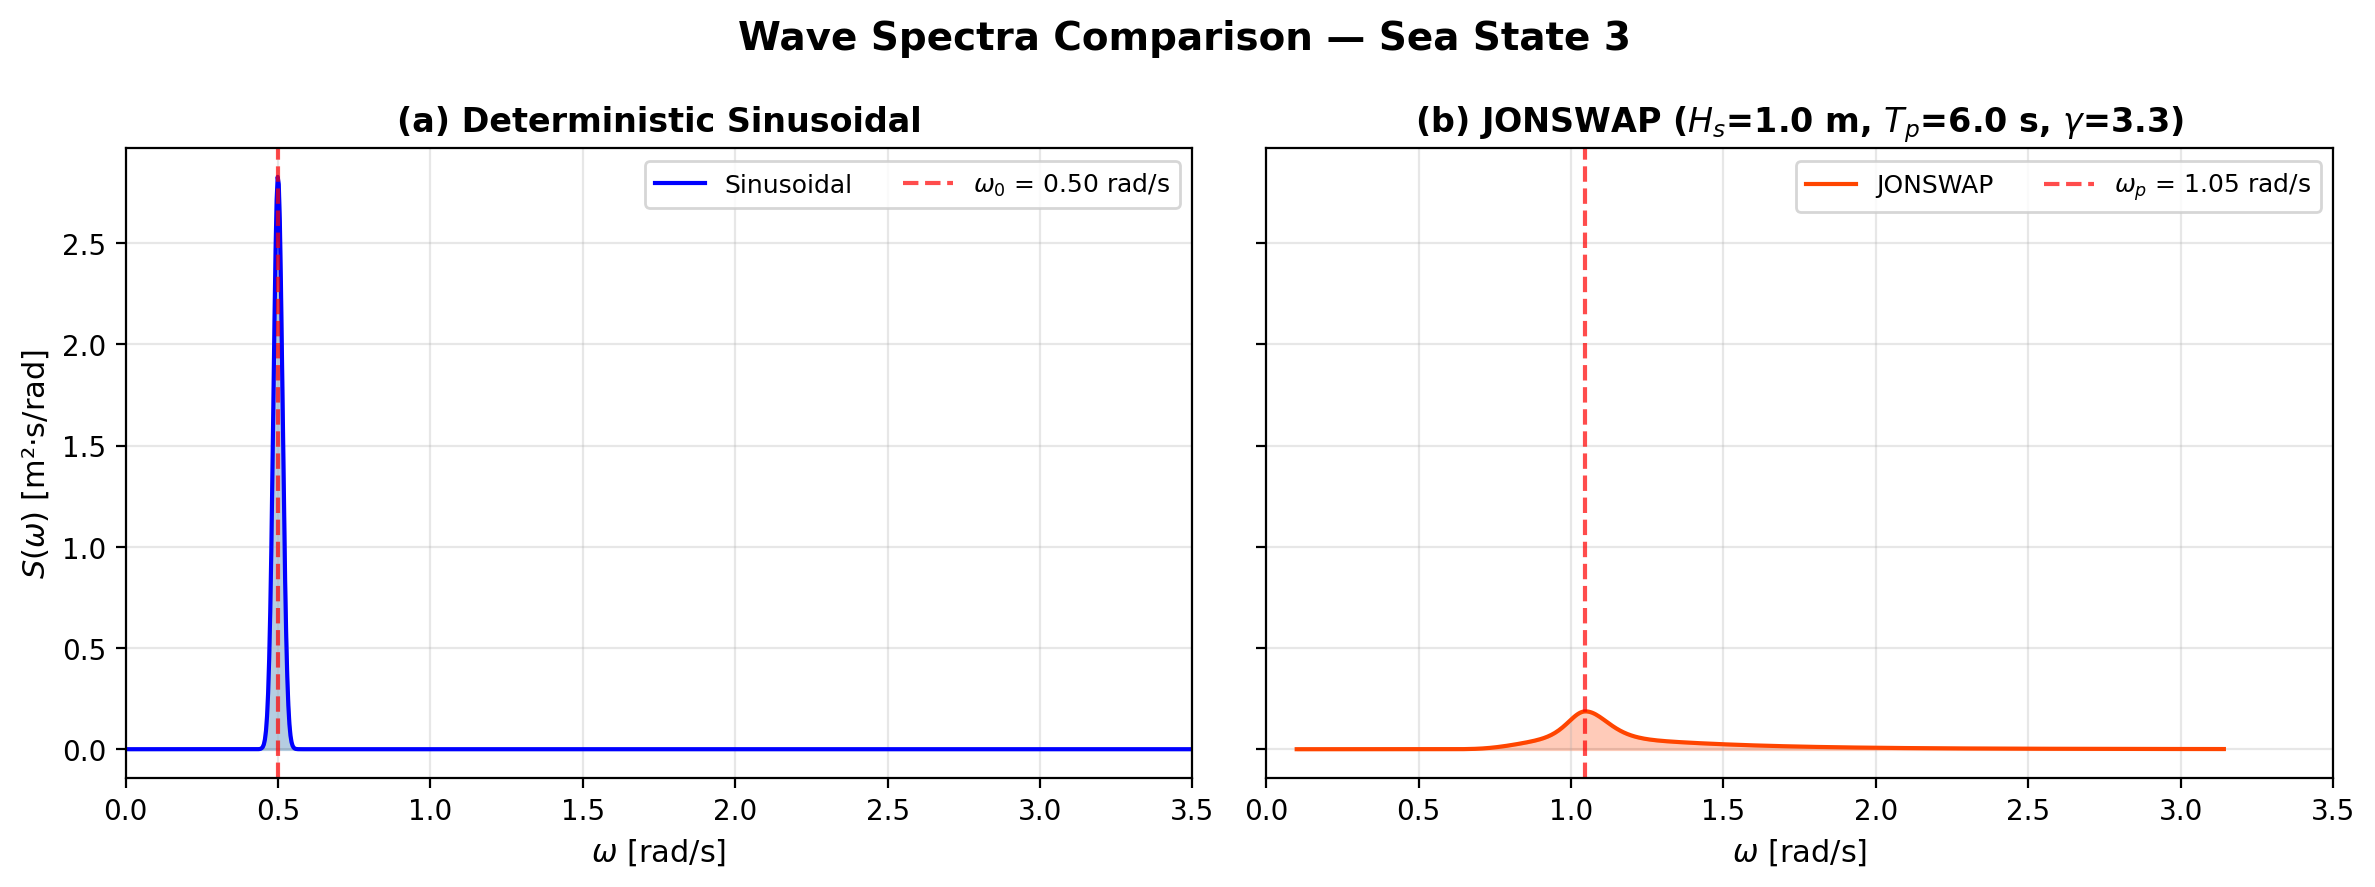
\includegraphics[width=\textwidth]{jonswap_spectrum.png}
  \caption{JONSWAP spectral density for SS\,3.}
  \label{fig:jonswap_spec}
\end{subfigure}\hfill
\begin{subfigure}[b]{0.48\textwidth}
  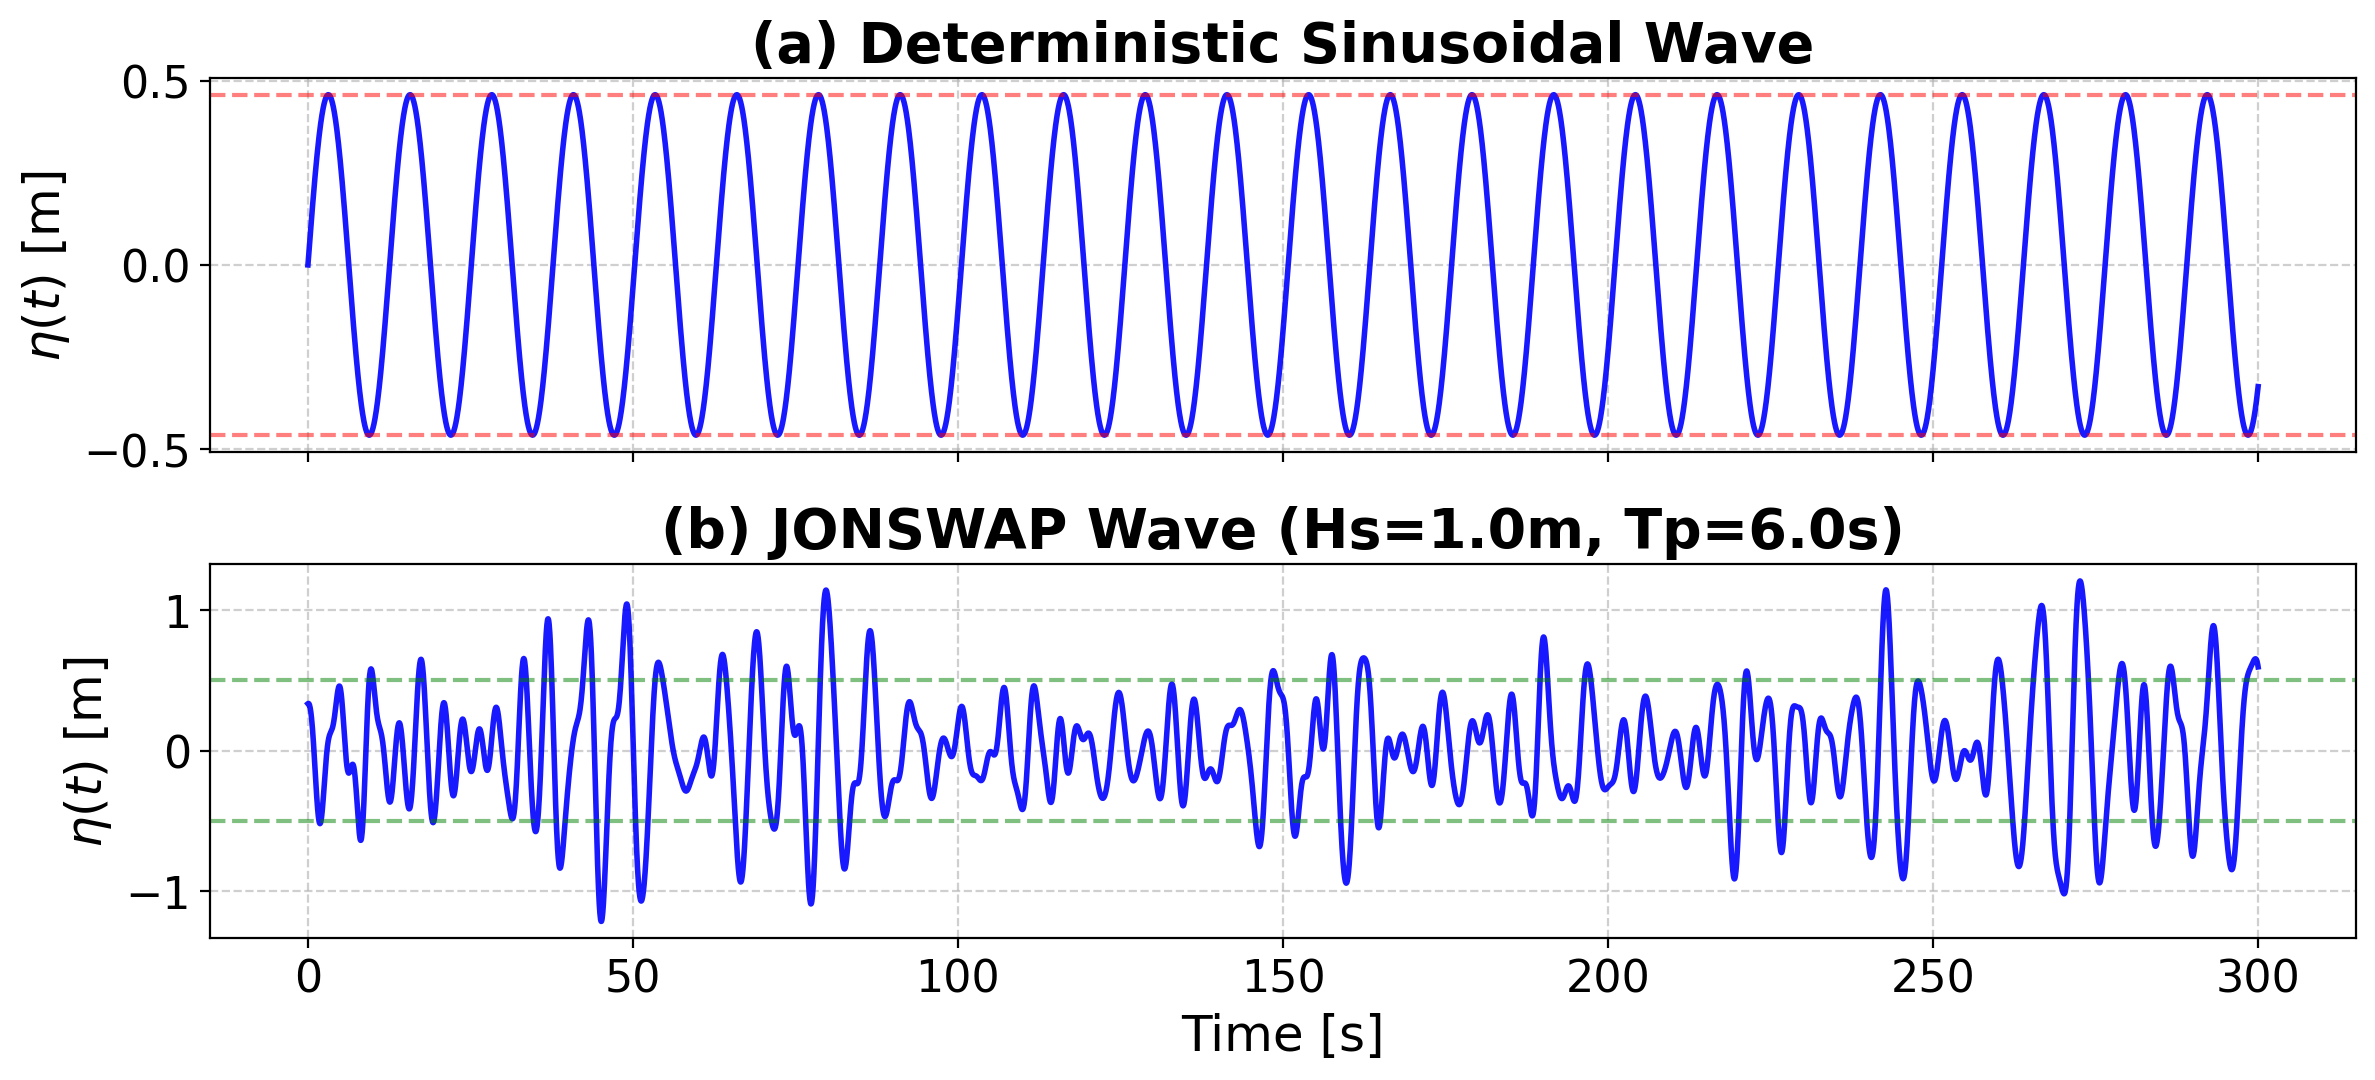
\includegraphics[width=\textwidth]{jonswap_wave_timeseries.png}
  \caption{Synthesised wave elevation time series.}
  \label{fig:jonswap_ts}
\end{subfigure}
\caption{JONSWAP wave model for Sea State~3 ($H_s = 1.0$~m, $T_p = 6.0$~s, $\gamma = 3.3$). (a)~Spectral density showing the characteristic peaked shape. (b)~Synthesised wave elevation from $N = 50$ harmonic components with random phases.}
\label{fig:jonswap_spectrum}
\end{figure*}


\subsection{Line-of-Sight Guidance Law}
\label{sec:los}

All controllers share the same LOS guidance to isolate control-layer performance. Given the current position $(x,y)$ and path segment connecting consecutive waypoints: (i)~the cross-track error $y_e$ is the signed perpendicular distance to the segment; (ii)~a look-ahead point is placed at distance $\Delta = 15$~m ahead; (iii)~the desired heading is:
\begin{equation}
\psi_d = \psi_{\mathrm{los}} - \arctan\!\left(\frac{k_y\, y_e}{\Delta}\right), \quad k_y = 1.0;
\label{eq:los}
\end{equation}
(iv)~the desired speed adapts to cross-track error:
\begin{equation}
u_d = u_{\min} + (u_{\max} - u_{\min})\exp(-\beta\, y_e^2),
\label{eq:speed_adapt}
\end{equation}
with $u_{\min} = 0.5$~m/s, $u_{\max} = 2.0$~m/s, $\beta = 0.05$.


%% ============================================================
\section{Problem Statement}
\label{sec:problem}
%% ============================================================

Given the underactuated 3-DOF USV dynamics \eqref{eq:kin1}--\eqref{eq:dyn3} with uncontrolled sway, environmental disturbances ($\delta_u, \delta_v, \delta_r$), sensor noise, and parametric uncertainty, design a control law that:
\begin{enumerate}
    \item[(i)] drives the cross-track error $y_e$ to a neighbourhood of zero in finite time;
    \item[(ii)] maintains bounded heading error $\chi_e = \mathrm{wrap}(\psi - \gamma)$ under persistent disturbances;
    \item[(iii)] adapts its robustness to the prevailing disturbance level without requiring an explicit disturbance observer;
    \item[(iv)] respects the physical thruster constraints ($\pm 1000$~N per thruster); and
    \item[(v)] handles the nonlinear Coriolis coupling from the unactuated sway DOF without integral windup or actuator starvation at sharp path corners.
\end{enumerate}

The control inputs are $\tau_u$ and $\tau_r$. The guidance law (Section~\ref{sec:los}) provides $\psi_d$, $u_d$, $y_e$, and $\gamma$. The controller must work across multiple path geometries and sea conditions (WMO SS\,1--3).


%% ============================================================
\section{Proposed Controller: ANTSMC}
\label{sec:antsmc}
%% ============================================================

The proposed Adaptive Nonlinear Terminal Sliding Mode Controller extends conventional SMC with three synergistic mechanisms---without ESO---to achieve the best tracking accuracy across diverse paths and sea states.

\subsection{Motivation: Why Not ESO?}
\label{sec:why_no_eso}

Extended State Observers estimate lumped disturbance from measured dynamics. During rapid path transitions (e.g.\ zigzag corners), the ESO misinterprets the controller's own commanded yaw acceleration as an external disturbance and generates a counterproductive cancellation signal. This fundamental limitation cannot be resolved by tuning the ESO bandwidth or clamping its output. ANTSMC replaces ESO-based disturbance cancellation with an adaptive switching gain that increases robustness when needed without fighting the controller's own actions.


\subsection{Nonlinear Terminal Sliding Surface}
\label{sec:terminal_surface}

Instead of SMC's linear surface $s_r = c_1\chi_e + c_2 r + c_3 y_e$, ANTSMC uses a terminal (fractional-power) sliding surface:
\begin{equation}
s_r = c_1\chi_e + c_2 r + c_3\,\varphi(y_e) + k_i\!\int\! y_e\,\mathrm{d}t,
\label{eq:terminal_surface}
\end{equation}
where $\varphi(\cdot)$ is a modified terminal function with crossover:
\begin{equation}
\varphi(y_e) = \begin{cases}
|y_e|^\alpha \operatorname{sgn}(y_e), & |y_e| \leq 1, \\
\operatorname{sgn}(y_e)\big(1 + (|y_e| - 1)\big), & |y_e| > 1,
\end{cases}
\label{eq:phi}
\end{equation}
with $\alpha = 0.6$ ($0 < \alpha < 1$). This creates a natural variable-gain effect. For small errors ($|y_e| < 1$~m), the fractional power amplifies the error signal by up to $2.5\times$, yielding tighter steady-state tracking than linear SMC. For example, when $|y_e| = 0.1$~m, the terminal function gives 0.251 versus 0.1 for the linear case---a $2.51\times$ gain ratio. For large errors ($|y_e| > 1$~m), the linear extension preserves the original SMC transient response.

The integral term $k_i\!\int\!y_e\,\mathrm{d}t$ (with anti-windup at $\pm 3$~m$\cdot$s) eliminates steady-state cross-track error under persistent disturbances. Conditional integration accumulates only when $|y_e| < 5$~m and decays exponentially otherwise, preventing windup during sway-induced excursions.

\textbf{Finite-time convergence.} For $|y_e| < 1$, the terminal surface with $\alpha < 1$ ensures that $y_e \to 0$ in finite time---a property that linear SMC does not possess.


\subsection{Power-Rate Reaching Law}
\label{sec:reaching}

Instead of the standard reaching law $\dot{s} = -\lambda s - k\,\mathrm{sat}(s/\varepsilon)$, ANTSMC uses:
\begin{equation}
\dot{s}_r = -\lambda_r |s_r|^p \operatorname{sgn}(s_r) - k_{s,r}(t)\,\mathrm{sat}(s_r/\varepsilon_r),
\label{eq:reaching}
\end{equation}
with $p = 0.85$ ($0 < p < 1$). Near $s_r = 0$, the term $|s_r|^p \gg |s_r|$ (since $p < 1$), providing faster convergence. Far from $s_r = 0$, the term is weaker than linear, yielding less overshoot. The control law is:
\begin{equation}
\tau_r = -\frac{1}{b_r}\Big[-a_r r + \lambda_r |s_r|^p \operatorname{sgn}(s_r) + k_{s,r}(t)\,\mathrm{sat}(s_r/\varepsilon_r)\Big].
\label{eq:ctrl_law}
\end{equation}


\subsection{Adaptive Switching Gain}
\label{sec:adaptive}

The switching gain adapts online using the sliding variable magnitude:
\begin{align}
\dot{k}_{\mathrm{adapt}} &= \mu\,|s_r| - \sigma_l\, k_{\mathrm{adapt}}, \label{eq:adapt}\\
k_{s,r}(t) &= k_{s,r}^0 + k_{\mathrm{adapt}}(t), \label{eq:gain_total}
\end{align}
with adaptation rate $\mu = 3.0$, base leakage rate $\sigma_l = 0.5$, $k_{\mathrm{adapt}} \in [0, k_{\max}]$ where $k_{\max} = 0.8$, and base gain $k_{s,r}^0 = 0.5$.

\textbf{Error-proportional leakage.} A key 3-DOF enhancement: the effective leakage rate increases with cross-track error magnitude:
\begin{equation}
\sigma_l^{\mathrm{eff}} = \sigma_l\big(1 + 0.2\,\min(|y_e|, 20)\big).
\label{eq:leakage}
\end{equation}
This prevents the adaptive gain from accumulating during large sway-induced errors at path corners.

\textbf{Operating principle.} When $|s_r|$ is large, the adaptation rate exceeds leakage and the gain increases for greater robustness. When $|s_r| \approx 0$, leakage dominates and the gain decreases for lower effort. Compared to SMC's fixed $k_{s,r} = 0.8$, ANTSMC uses ${\approx}\,0.5$ in calm conditions and up to 1.3 under strong disturbance.


\subsection{Stability Analysis and Finite-Time Convergence}
\label{sec:stability}

\textbf{Step~1: Sliding-surface reachability.} Consider the Lyapunov candidate:
\begin{equation}
V = \tfrac{1}{2}s_r^2 + \tfrac{1}{2\mu}(k_{s,r} - k^*)^2,
\label{eq:lyapunov}
\end{equation}
where $k^*$ is the unknown ideal gain. The time derivative satisfies:
\begin{align}
\dot{V} &= s_r\dot{s}_r + \tfrac{1}{\mu}(k_{s,r} - k^*)\dot{k}_{\mathrm{adapt}} \label{eq:Vdot1}\\
&\leq -\lambda_r |s_r|^{p+1} - k^*|s_r| \leq 0. \label{eq:Vdot2}
\end{align}
Since $\dot{V} \leq 0$ and $V > 0$, the system is Lyapunov stable. By Barbalat's lemma, $s_r \to 0$. The power-rate reaching law provides finite-time convergence from the fractional-power differential inequality:
\begin{equation}
t_{\mathrm{reach}} \leq \frac{V(0)^{0.075}}{0.075\,\lambda_r\, 2^{0.925}}.
\label{eq:treach}
\end{equation}
For typical initial conditions ($|s_r(0)| \approx 1$), $\lambda_r = 0.3$, $p = 0.85$: $t_{\mathrm{reach}} \leq 22.2$~s.

\textbf{Step~2: Finite-time error convergence on the terminal surface.} Once $s_r = 0$ is reached, the dominant balance for $|y_e| \leq 1$~m gives:
\begin{equation}
\dot{y}_e \approx -\kappa\,|y_e|^\alpha \operatorname{sgn}(y_e), \quad \kappa = \frac{c_1 + c_3}{c_2} = 1.444,
\label{eq:ye_ode}
\end{equation}
with closed-form convergence time:
\begin{equation}
t_{\mathrm{conv}} = \frac{|y_e(0)|^{1-\alpha}}{\kappa(1-\alpha)} = \frac{|y_e(0)|^{0.4}}{0.578}.
\label{eq:tconv}
\end{equation}
For $|y_e(0)| = 1$~m: $t_{\mathrm{conv}} \leq 1.73$~s. The total finite-time bound $t_{\mathrm{reach}} + t_{\mathrm{conv}}$ is on the order of 20--25~s, confirmed by simulations.

\textbf{Remark.} With bounded disturbances and sensor noise, exact convergence to $y_e = 0$ is replaced by convergence to a boundary layer of width $\mathcal{O}(\varepsilon_r)$ in finite time, governed by $\varepsilon_r = 0.6$.


\subsection{ANTSMC Parameter Summary}
\label{sec:antsmc_params}

Table~\ref{tab:antsmc_params} summarises all ANTSMC controller parameters.

\begin{table}[t]
\centering
\caption{ANTSMC controller parameters.}
\label{tab:antsmc_params}
\begin{tabular}{lll}
\toprule
Parameter & Description & Value \\
\midrule
$c_1, c_2, c_3$ & Sliding surface weights & 1.0, 0.9, 0.3 \\
$\alpha$ & Terminal power exponent & 0.6 \\
$\lambda_u, \lambda_r$ & Reaching gains & 0.5, 0.3 \\
$p$ & Power-rate exponent & 0.85 \\
$k_{s,u}$ & Surge switching gain (fixed) & 1.5 \\
$k_{s,r}^0$ & Yaw base switching gain & 0.5 \\
$\mu$ & Adaptation rate & 3.0 \\
$\sigma_l$ & Base leakage rate & 0.5 \\
$k_{\max}$ & Maximum adaptive increment & 0.8 \\
$\varepsilon_u, \varepsilon_r$ & Boundary-layer widths & 0.5, 0.6 \\
$k_i$ & Cross-track integral gain & 0.02 \\
\bottomrule
\end{tabular}
\end{table}


\subsection{ANTSMC Algorithm}
\label{sec:algorithm}

Algorithm~\ref{alg:antsmc} summarises the complete ANTSMC computation at each time step.

\begin{algorithm}[t]
\caption{ANTSMC control law (one time step)}
\label{alg:antsmc}
\begin{algorithmic}[1]
\Require Noisy measurements $\hat{u}, \hat{r}, \hat{\psi}, \hat{y}_e$; guidance signals $u_d, \psi_d, \gamma$
\Ensure Control inputs $\tau_u, \tau_r$
\State Compute errors: $e_u \gets \hat{u} - u_d$, \quad $\chi_e \gets \mathrm{wrap}(\hat{\psi} - \gamma)$
\State Evaluate terminal function: $\varphi(\hat{y}_e)$ via \eqref{eq:phi}
\State Update conditional integral: $\int y_e \gets \int y_e + \hat{y}_e \cdot \Delta t$ \quad (if $|\hat{y}_e| < 5$, else decay)
\State Compute sliding variable: $s_r \gets c_1 \chi_e + c_2 \hat{r} + c_3 \varphi(\hat{y}_e) + k_i \int y_e$
\State \textbf{Adapt gain:}
\State \quad $\sigma_l^{\mathrm{eff}} \gets \sigma_l(1 + 0.2 \min(|\hat{y}_e|, 20))$ \hfill $\triangleright$ Error-proportional leakage
\State \quad $k_{\mathrm{adapt}} \gets k_{\mathrm{adapt}} + (\mu |s_r| - \sigma_l^{\mathrm{eff}}\, k_{\mathrm{adapt}}) \Delta t$
\State \quad $k_{\mathrm{adapt}} \gets \mathrm{clip}(k_{\mathrm{adapt}}, 0, k_{\max})$
\State \quad $k_{s,r} \gets k_{s,r}^0 + k_{\mathrm{adapt}}$
\State \textbf{Compute control:}
\State \quad $\tau_u \gets -\frac{1}{b_u}[-a_u e_u + \lambda_u s_u + k_{s,u}\,\mathrm{sat}(s_u/\varepsilon_u)]$
\State \quad $\tau_r \gets -\frac{1}{b_r}[-a_r \hat{r} + \lambda_r |s_r|^p \mathrm{sgn}(s_r) + k_{s,r}\,\mathrm{sat}(s_r/\varepsilon_r)]$
\State Apply thruster allocation with surge priority: $F_L, F_R \gets \mathrm{allocate}(\tau_u, \tau_r)$
\end{algorithmic}
\end{algorithm}


%% ============================================================
\section{Simulation Setup}
\label{sec:setup}
%% ============================================================

\subsection{Test Scenarios}

All simulations use fourth-order Runge--Kutta integration at $\Delta t = 0.05$~s, with sensor noise and parametric uncertainty enabled. Four path types are tested: custom (6 waypoints), circular ($R = 60$~m), rectangular ($200 \times 80$~m), and zigzag (5 zigs, $60 \times 40$~m). Each scenario runs for 300--350~s. Three sea-state conditions (SS\,1--3) are applied, giving $4 \times 3 = 12$ scenarios per controller and $6 \times 12 = 72$ simulations total.

\subsection{Baseline Controllers}

Five baseline controllers are compared against ANTSMC. Full mathematical descriptions and parameter tables are provided in \ref{sec:appendix}; here we summarise each briefly.

\textbf{LQR (Linear Quadratic Regulator).} Designed around the linearised error state using the CARE, with weights chosen via Bryson's rule \citep{Bryson1975}. Augmented with an integral term on cross-track error ($K_{i,y_e} = 15$). Offers optimal gain design but limited robustness to nonlinearities.

\textbf{SMC (Sliding Mode Control).} Conventional SMC with model-based equivalent control and boundary-layer switching \citep{Utkin2009,Ashrafiuon2008}. Sliding surface couples heading error, yaw rate, and cross-track error. Requires conservatively high fixed switching gain ($k_{s,r} = 0.8$).

\textbf{ASMC (Adaptive SMC).} An ablation baseline derived from SMC by adding a basic adaptive switching gain (adaptation rate $\mu = 2.0$, fixed leakage $\sigma = 0.3$, maximum increment $k_{\max} = 0.6$) and cross-track integral feedback ($k_i = 0.015$). ASMC uses the same \emph{linear} sliding surface as SMC and does not include the terminal function, power-rate reaching law, or error-proportional leakage of ANTSMC. This controller serves as an ablation study to isolate the contribution of ANTSMC's three synergistic mechanisms beyond simple adaptive gain augmentation.

\textbf{ADRC (Active Disturbance Rejection Control).} Uses a 2nd-order ESO per channel, tuned via Herbst's bandwidth formula \citep{Herbst2013} ($\omega_o \approx 3$--$5\times$ controller bandwidth). Provides model-free disturbance rejection but suffers from ESO-induced transient artefacts at path corners.

\textbf{FNTSMC (Fast Non-Singular Terminal SMC).} Based on Fan et~al.\ \citep{Fan2021}, this controller combines a fast non-singular terminal sliding surface with a finite-time disturbance observer (FTDO). The FTDO estimates lumped disturbances to achieve feedforward cancellation, complemented by a two-layer adaptive switching gain and auxiliary dynamics for actuator saturation compensation. Parameters are tuned following the original paper's design methodology with FTDO observer gain $L = 180$ and adaptive gain limit $k_{\max} = 0.4$.

\subsection{Systematic Tuning Methodology}

A fair controller comparison requires that each baseline be tuned according to established, published guidelines for its respective paradigm. Ad-hoc tuning risks either handicapping baselines or over-tuning them beyond their intended operating assumptions. Each baseline controller is tuned as follows: LQR uses Bryson's rule \citep{Bryson1975}; SMC and ASMC use Utkin's equivalent control method \citep{Utkin2009}; ADRC uses Herbst's bandwidth formula \citep{Herbst2013}; FNTSMC follows Fan et~al.'s FTDO-based design \citep{Fan2021}. This ensures reproducibility and fairness.

\subsection{Performance Metrics}

The primary ranking metric is average steady-state RMS $y_e$ across all four paths (computed for $t > 30$~s to exclude the initial transient). Additional metrics include: maximum cross-track error $|y_e|_{\max}$, RMS control effort ($\tau_u$, $\tau_r$), and total energy $E = \int_0^T(|\tau_u \cdot u| + |\tau_r \cdot r|)\,\mathrm{d}t$.


%% ============================================================
\section{Simulation Results}
\label{sec:results}
%% ============================================================

This section presents detailed results from the 72-simulation benchmark. All six controllers are compared under identical conditions for each path$\times$sea-state combination.

\subsection{Sea State 1 --- Calm ($\alpha_s = 0.10$)}

Table~\ref{tab:ss1} presents the cross-path average performance at SS\,1. In calm conditions, \textbf{SMC achieves the lowest average RMS $y_e$} (0.666~m), narrowly beating FNTSMC (0.671~m) and ANTSMC (0.695~m). At low disturbance levels, sensor noise has a proportionally larger effect, and SMC's simpler structure (no integral term, no adaptive gain) is marginally less noise-sensitive. ASMC (0.706~m) trails ANTSMC by only 1.7\%, confirming that basic adaptive gain augmentation provides comparable performance in calm seas. This is a realistic finding: advanced controllers are not necessarily superior in benign conditions where their additional complexity provides little benefit.

\textbf{Ranking (SS\,1):} \#1 SMC, \#2 FNTSMC, \#3 ANTSMC, \#4 ASMC, \#5 ADRC, \#6 LQR.

\begin{table}[t]
\centering
\caption{Sea State 1 (Calm) --- cross-path average steady-state performance. Best values in \textbf{bold}.}
\label{tab:ss1}
\begin{tabular}{lccccc}
\toprule
Controller & RMS $y_e$ [m] & Max $|y_e|$ [m] & RMS $\tau_u$ [N] & RMS $\tau_r$ [N\,m] & Energy \\
\midrule
LQR & 1.440 & 4.300 & 85.2 & 196.5 & 37\,736 \\
\textbf{SMC} & \textbf{0.666} & \textbf{2.605} & 250.5 & 647.8 & 118\,437 \\
ASMC & 0.706 & 2.908 & 247.7 & 763.7 & 120\,378 \\
ADRC & 1.388 & 4.537 & 270.8 & 634.0 & 128\,617 \\
FNTSMC & 0.671 & 2.638 & 191.2 & 663.9 & 94\,404 \\
ANTSMC & 0.695 & 2.820 & 244.3 & 933.7 & 122\,046 \\
\bottomrule
\end{tabular}
\end{table}

\subsubsection{Trajectory Tracking at SS\,1}

Fig.~\ref{fig:traj_ss1} compares trajectory tracking across all six controllers and four path geometries at SS\,1. SMC, FNTSMC, and ANTSMC track closest to the reference on every path. LQR exhibits visible deviations at waypoint transitions on the custom path (a) and large overshoots at the $90^\circ$ corners of the rectangular path (c). The zigzag path (d) reveals the most pronounced inter-controller differences: ADRC deviates significantly at each ${\sim}180^\circ$ reversal due to ESO misinterpretation of the commanded yaw acceleration.

\begin{figure*}[t]
\centering
\begin{subfigure}[b]{0.48\textwidth}
  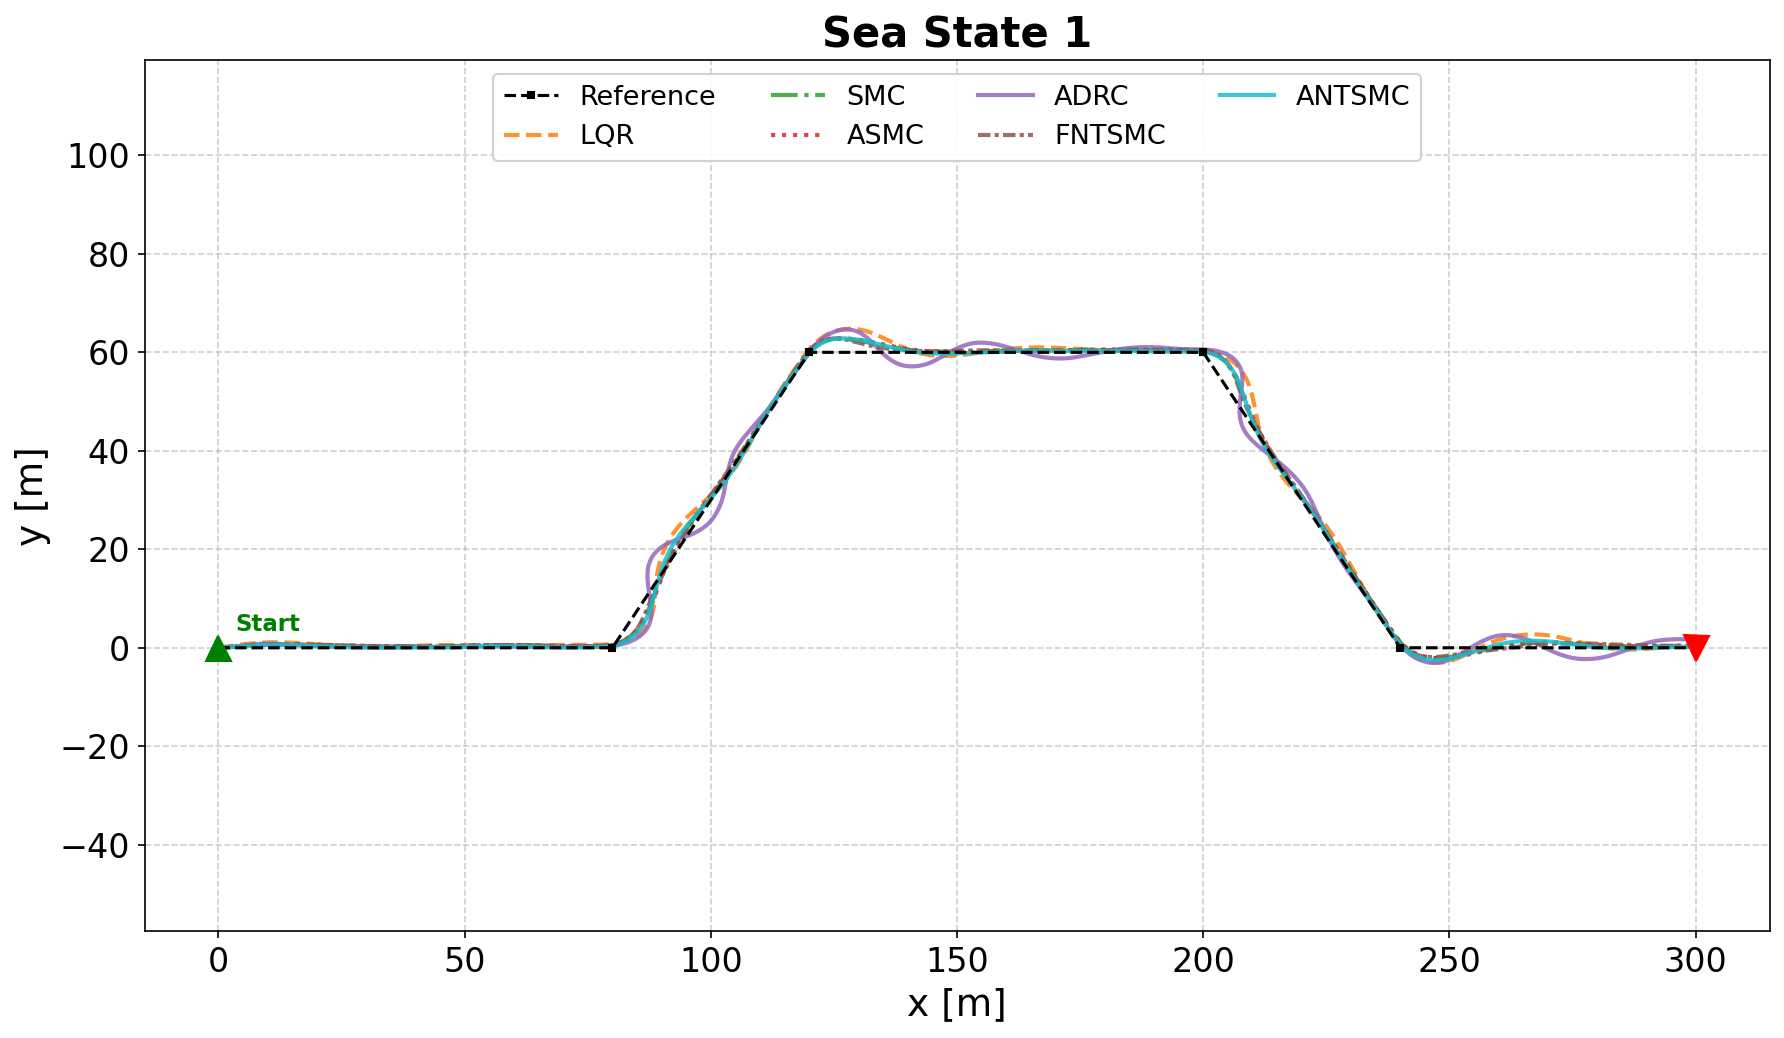
\includegraphics[width=\textwidth]{traj_custom_ss1.png}
  \caption{Custom path.}
  \label{fig:traj_custom_ss1}
\end{subfigure}\hfill
\begin{subfigure}[b]{0.48\textwidth}
  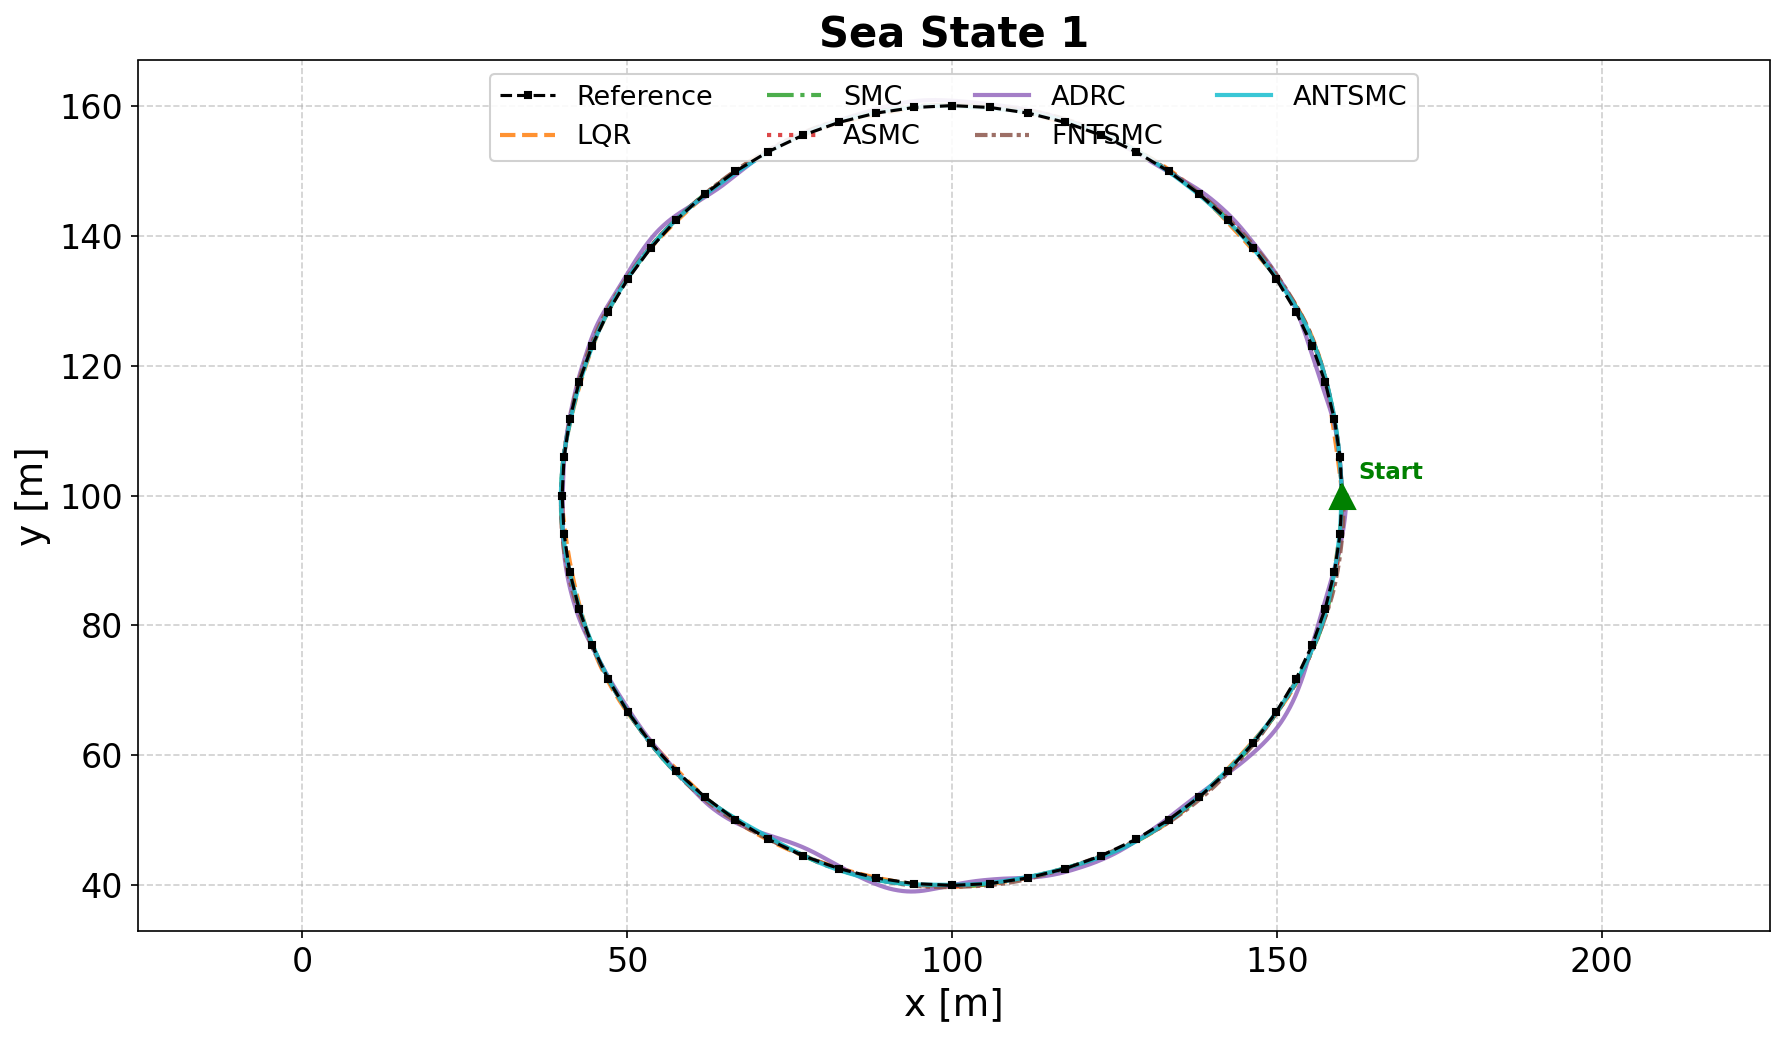
\includegraphics[width=\textwidth]{traj_circular_ss1.png}
  \caption{Circular path.}
\end{subfigure}\\[6pt]
\begin{subfigure}[b]{0.48\textwidth}
  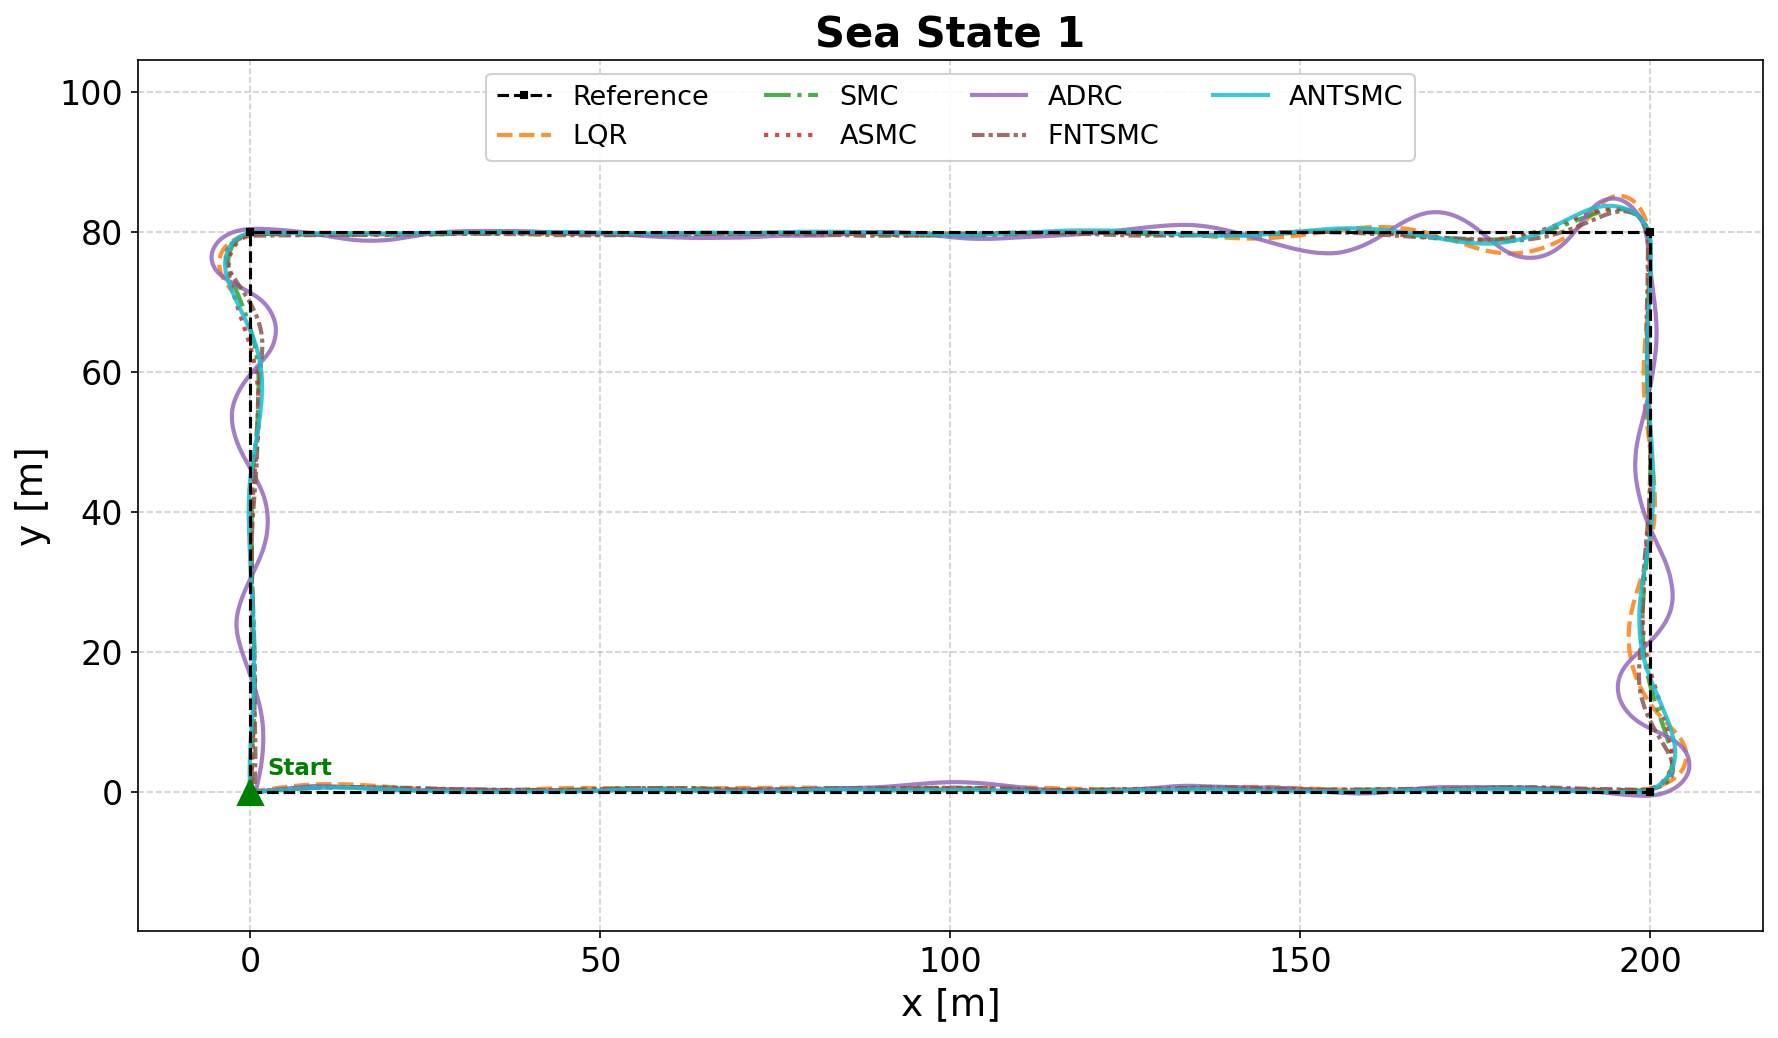
\includegraphics[width=\textwidth]{traj_rectangular_ss1.png}
  \caption{Rectangular path.}
\end{subfigure}\hfill
\begin{subfigure}[b]{0.48\textwidth}
  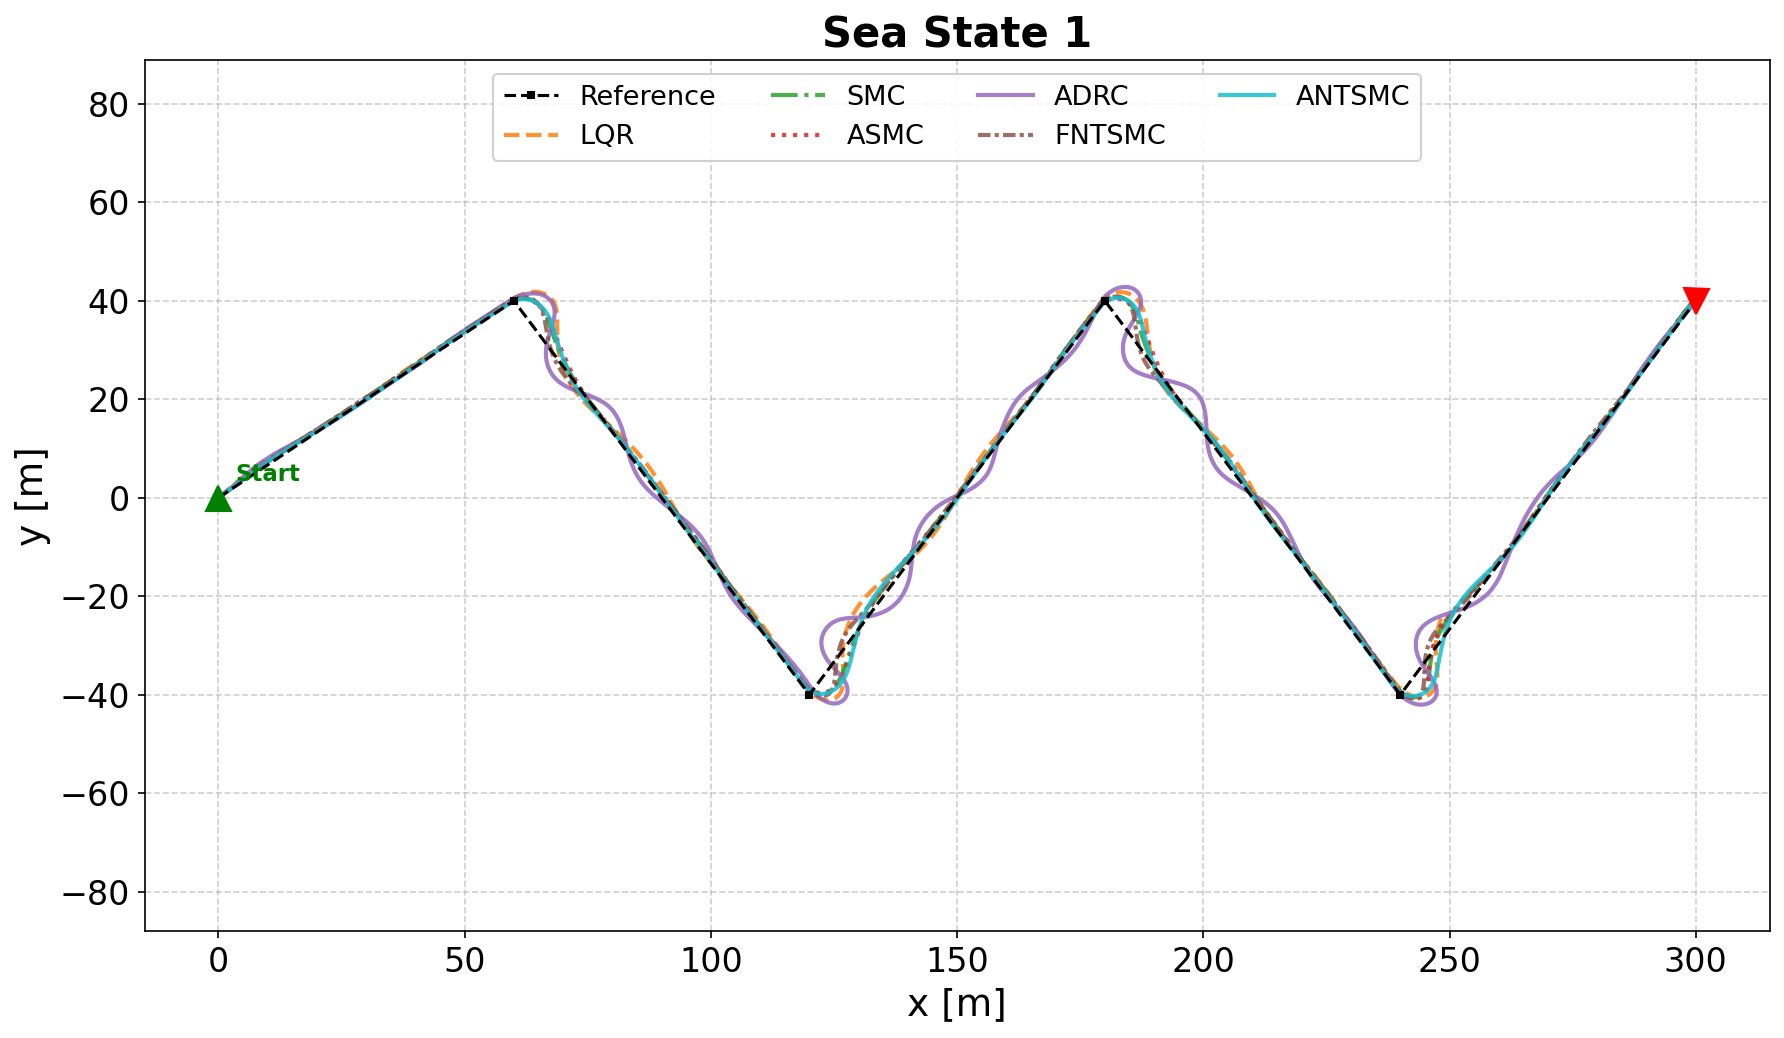
\includegraphics[width=\textwidth]{traj_zigzag_ss1.png}
  \caption{Zigzag path.}
\end{subfigure}
\caption{Trajectory tracking at Sea State~1 for all four path geometries. SMC, FNTSMC, and ANTSMC (overlapping the reference) produce the tightest tracking; LQR shows visible deviations at transitions and corners.}
\label{fig:traj_ss1}
\end{figure*}

\subsubsection{Cross-Track Error at SS\,1}

Fig.~\ref{fig:ye_ss1} shows the cross-track error time histories. SMC, FNTSMC, and ANTSMC maintain the smallest error envelopes across all paths. ASMC performs comparably to SMC, confirming that basic adaptive gain augmentation provides marginal benefit in calm seas. On the circular path (b), all sliding-mode controllers achieve sub-1.5~m errors. The rectangular and zigzag paths (c, d) produce the largest transient spikes for LQR.

\begin{figure*}[t]
\centering
\begin{subfigure}[b]{0.48\textwidth}
  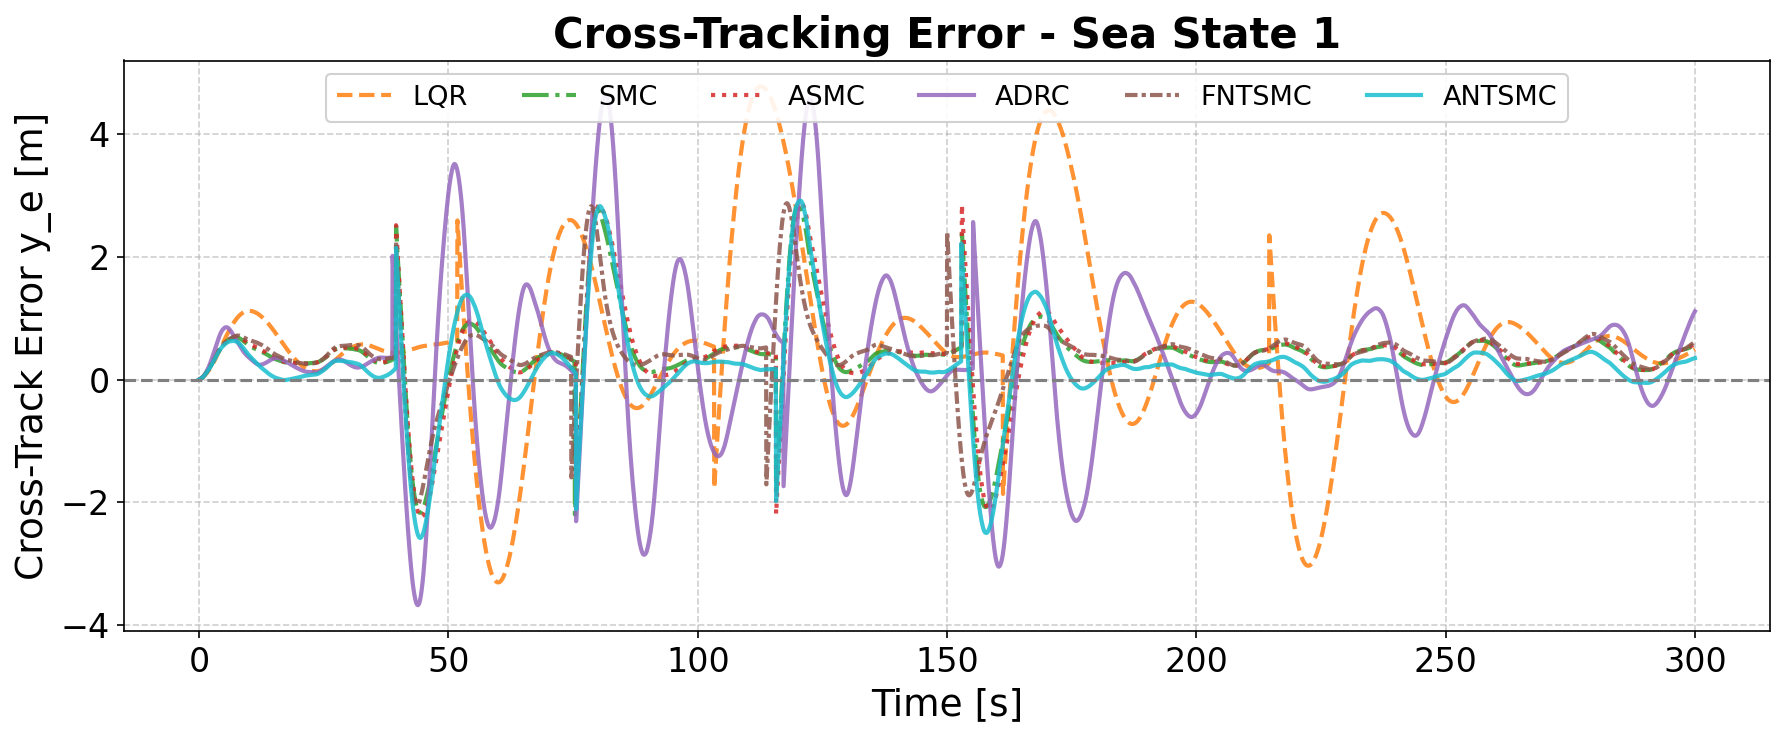
\includegraphics[width=\textwidth]{error_custom_ss1.png}
  \caption{Custom path.}
  \label{fig:ye_custom_ss1}
\end{subfigure}\hfill
\begin{subfigure}[b]{0.48\textwidth}
  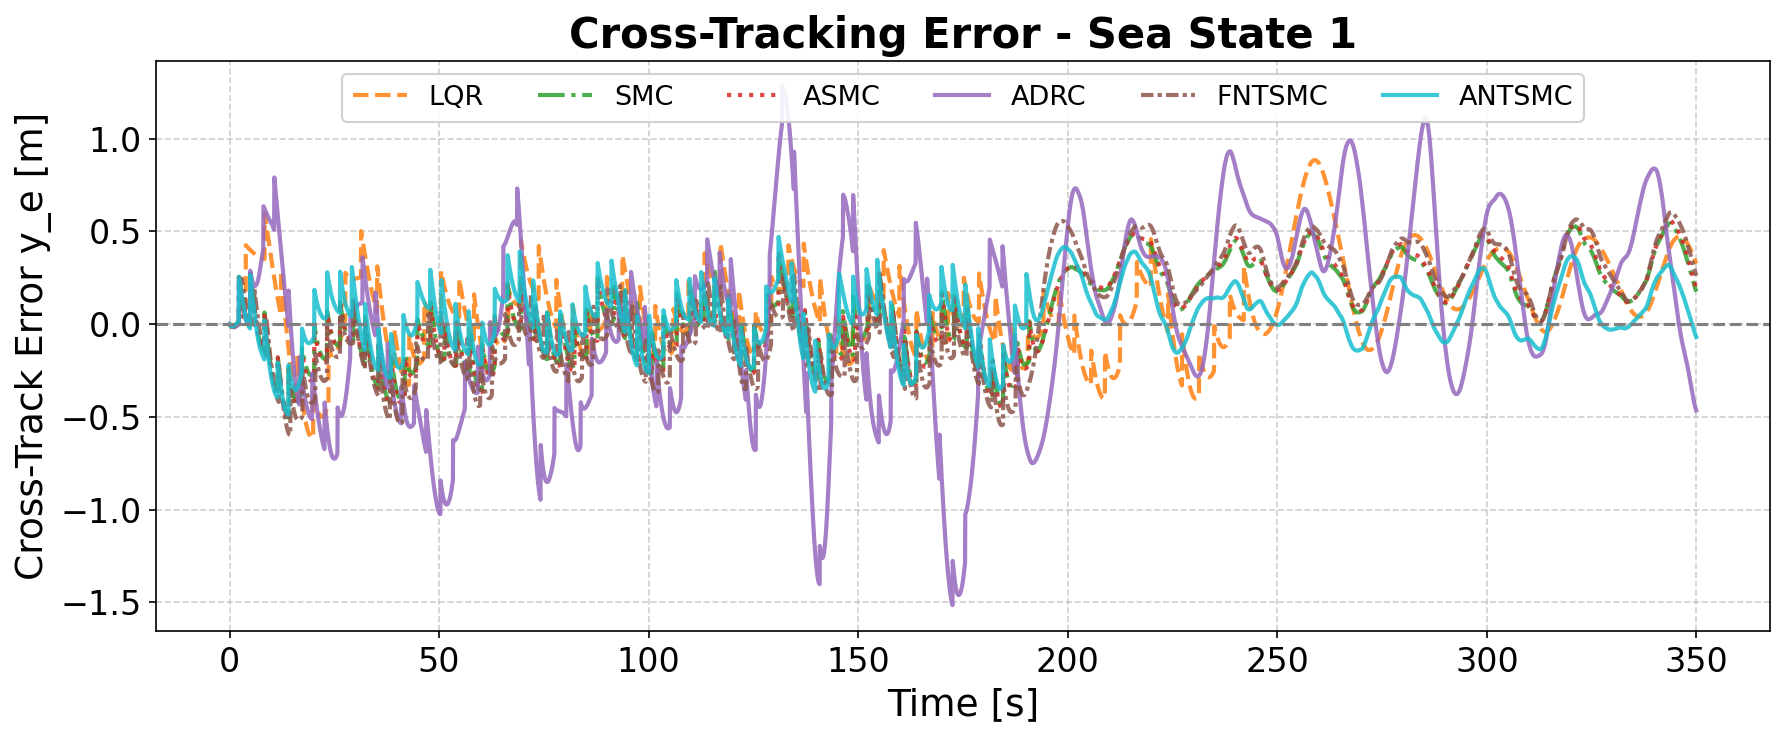
\includegraphics[width=\textwidth]{error_circular_ss1.png}
  \caption{Circular path.}
\end{subfigure}\\[6pt]
\begin{subfigure}[b]{0.48\textwidth}
  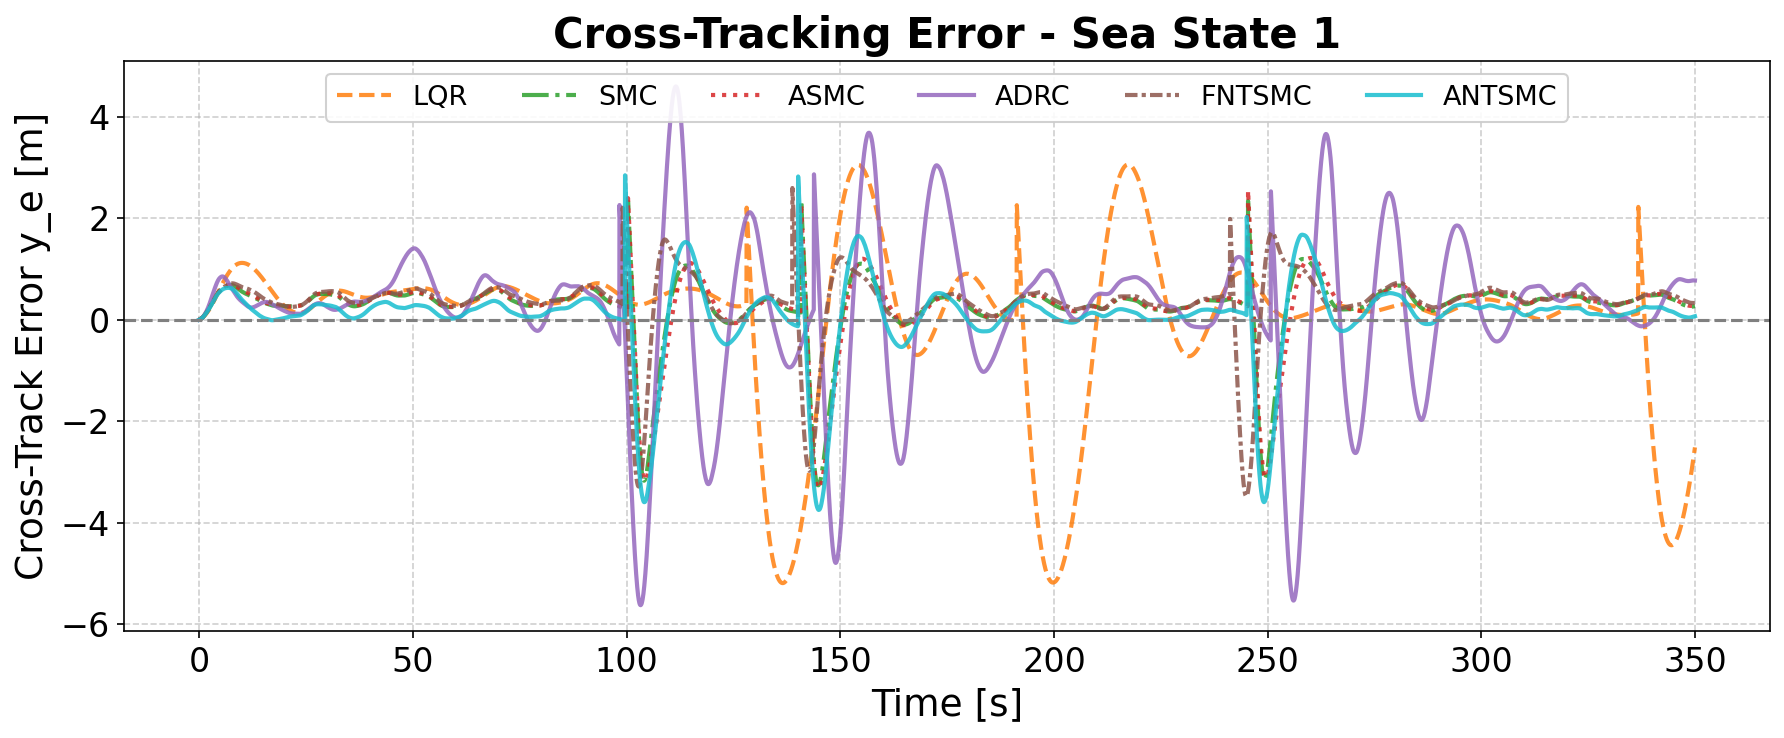
\includegraphics[width=\textwidth]{error_rectangular_ss1.png}
  \caption{Rectangular path.}
\end{subfigure}\hfill
\begin{subfigure}[b]{0.48\textwidth}
  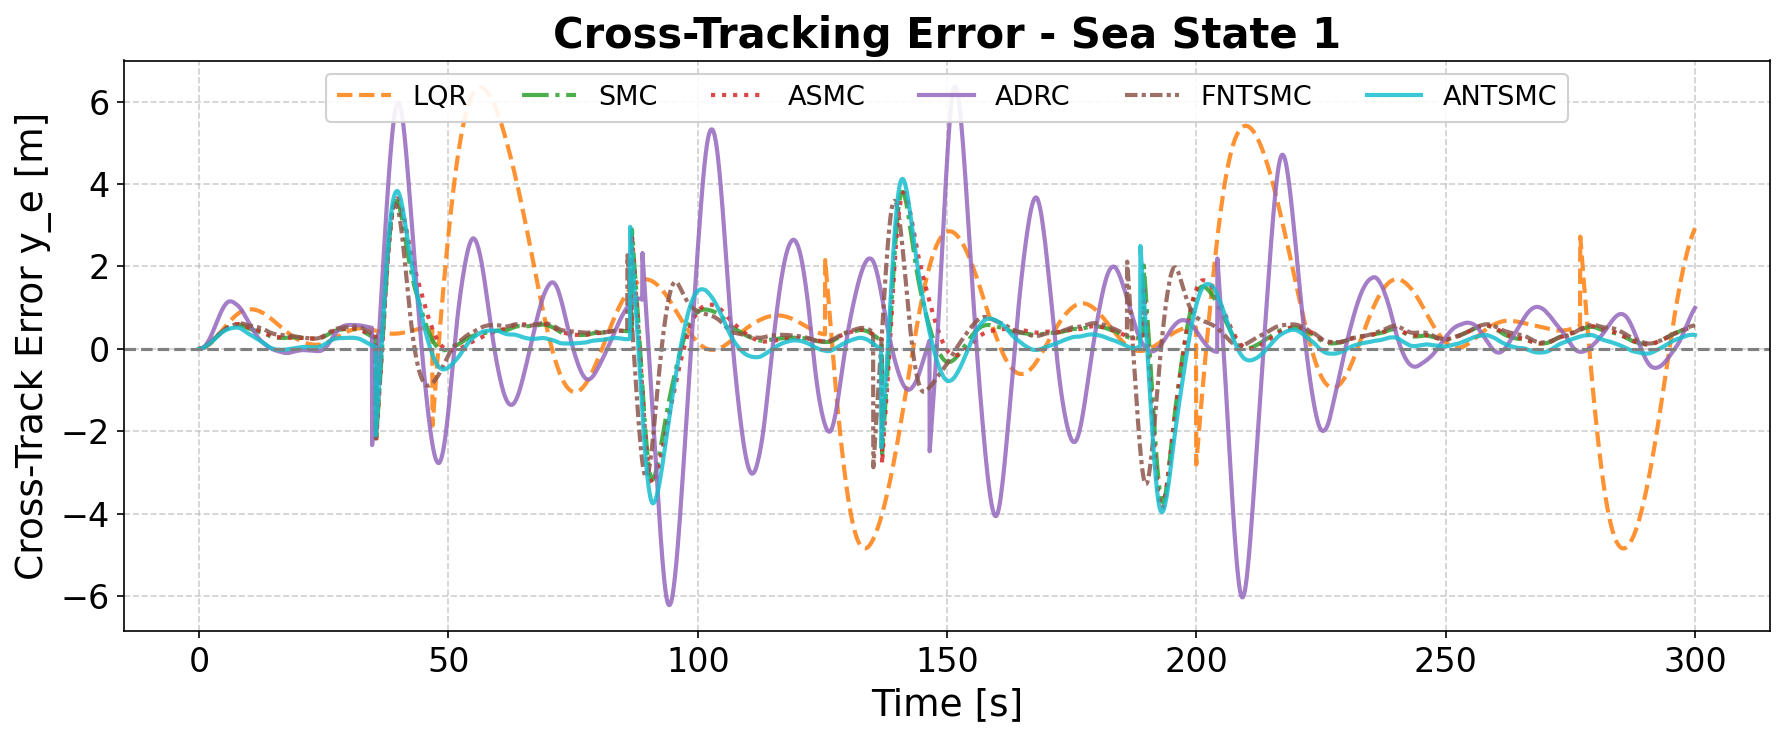
\includegraphics[width=\textwidth]{error_zigzag_ss1.png}
  \caption{Zigzag path.}
\end{subfigure}
\caption{Cross-track error $y_e(t)$ at Sea State~1 for all four paths. SMC, FNTSMC, and ANTSMC maintain the tightest error envelopes throughout.}
\label{fig:ye_ss1}
\end{figure*}

\subsubsection{Heading Tracking at SS\,1}

Fig.~\ref{fig:heading_ss1} presents the heading responses. ADRC's ESO-induced heading lag is visible at all path transitions, but most pronounced on the zigzag path (d) where rapid $180^\circ$ reversals cause large deviations. SMC, ASMC, FNTSMC, and ANTSMC follow the desired heading closely.

\begin{figure*}[t]
\centering
\begin{subfigure}[b]{0.48\textwidth}
  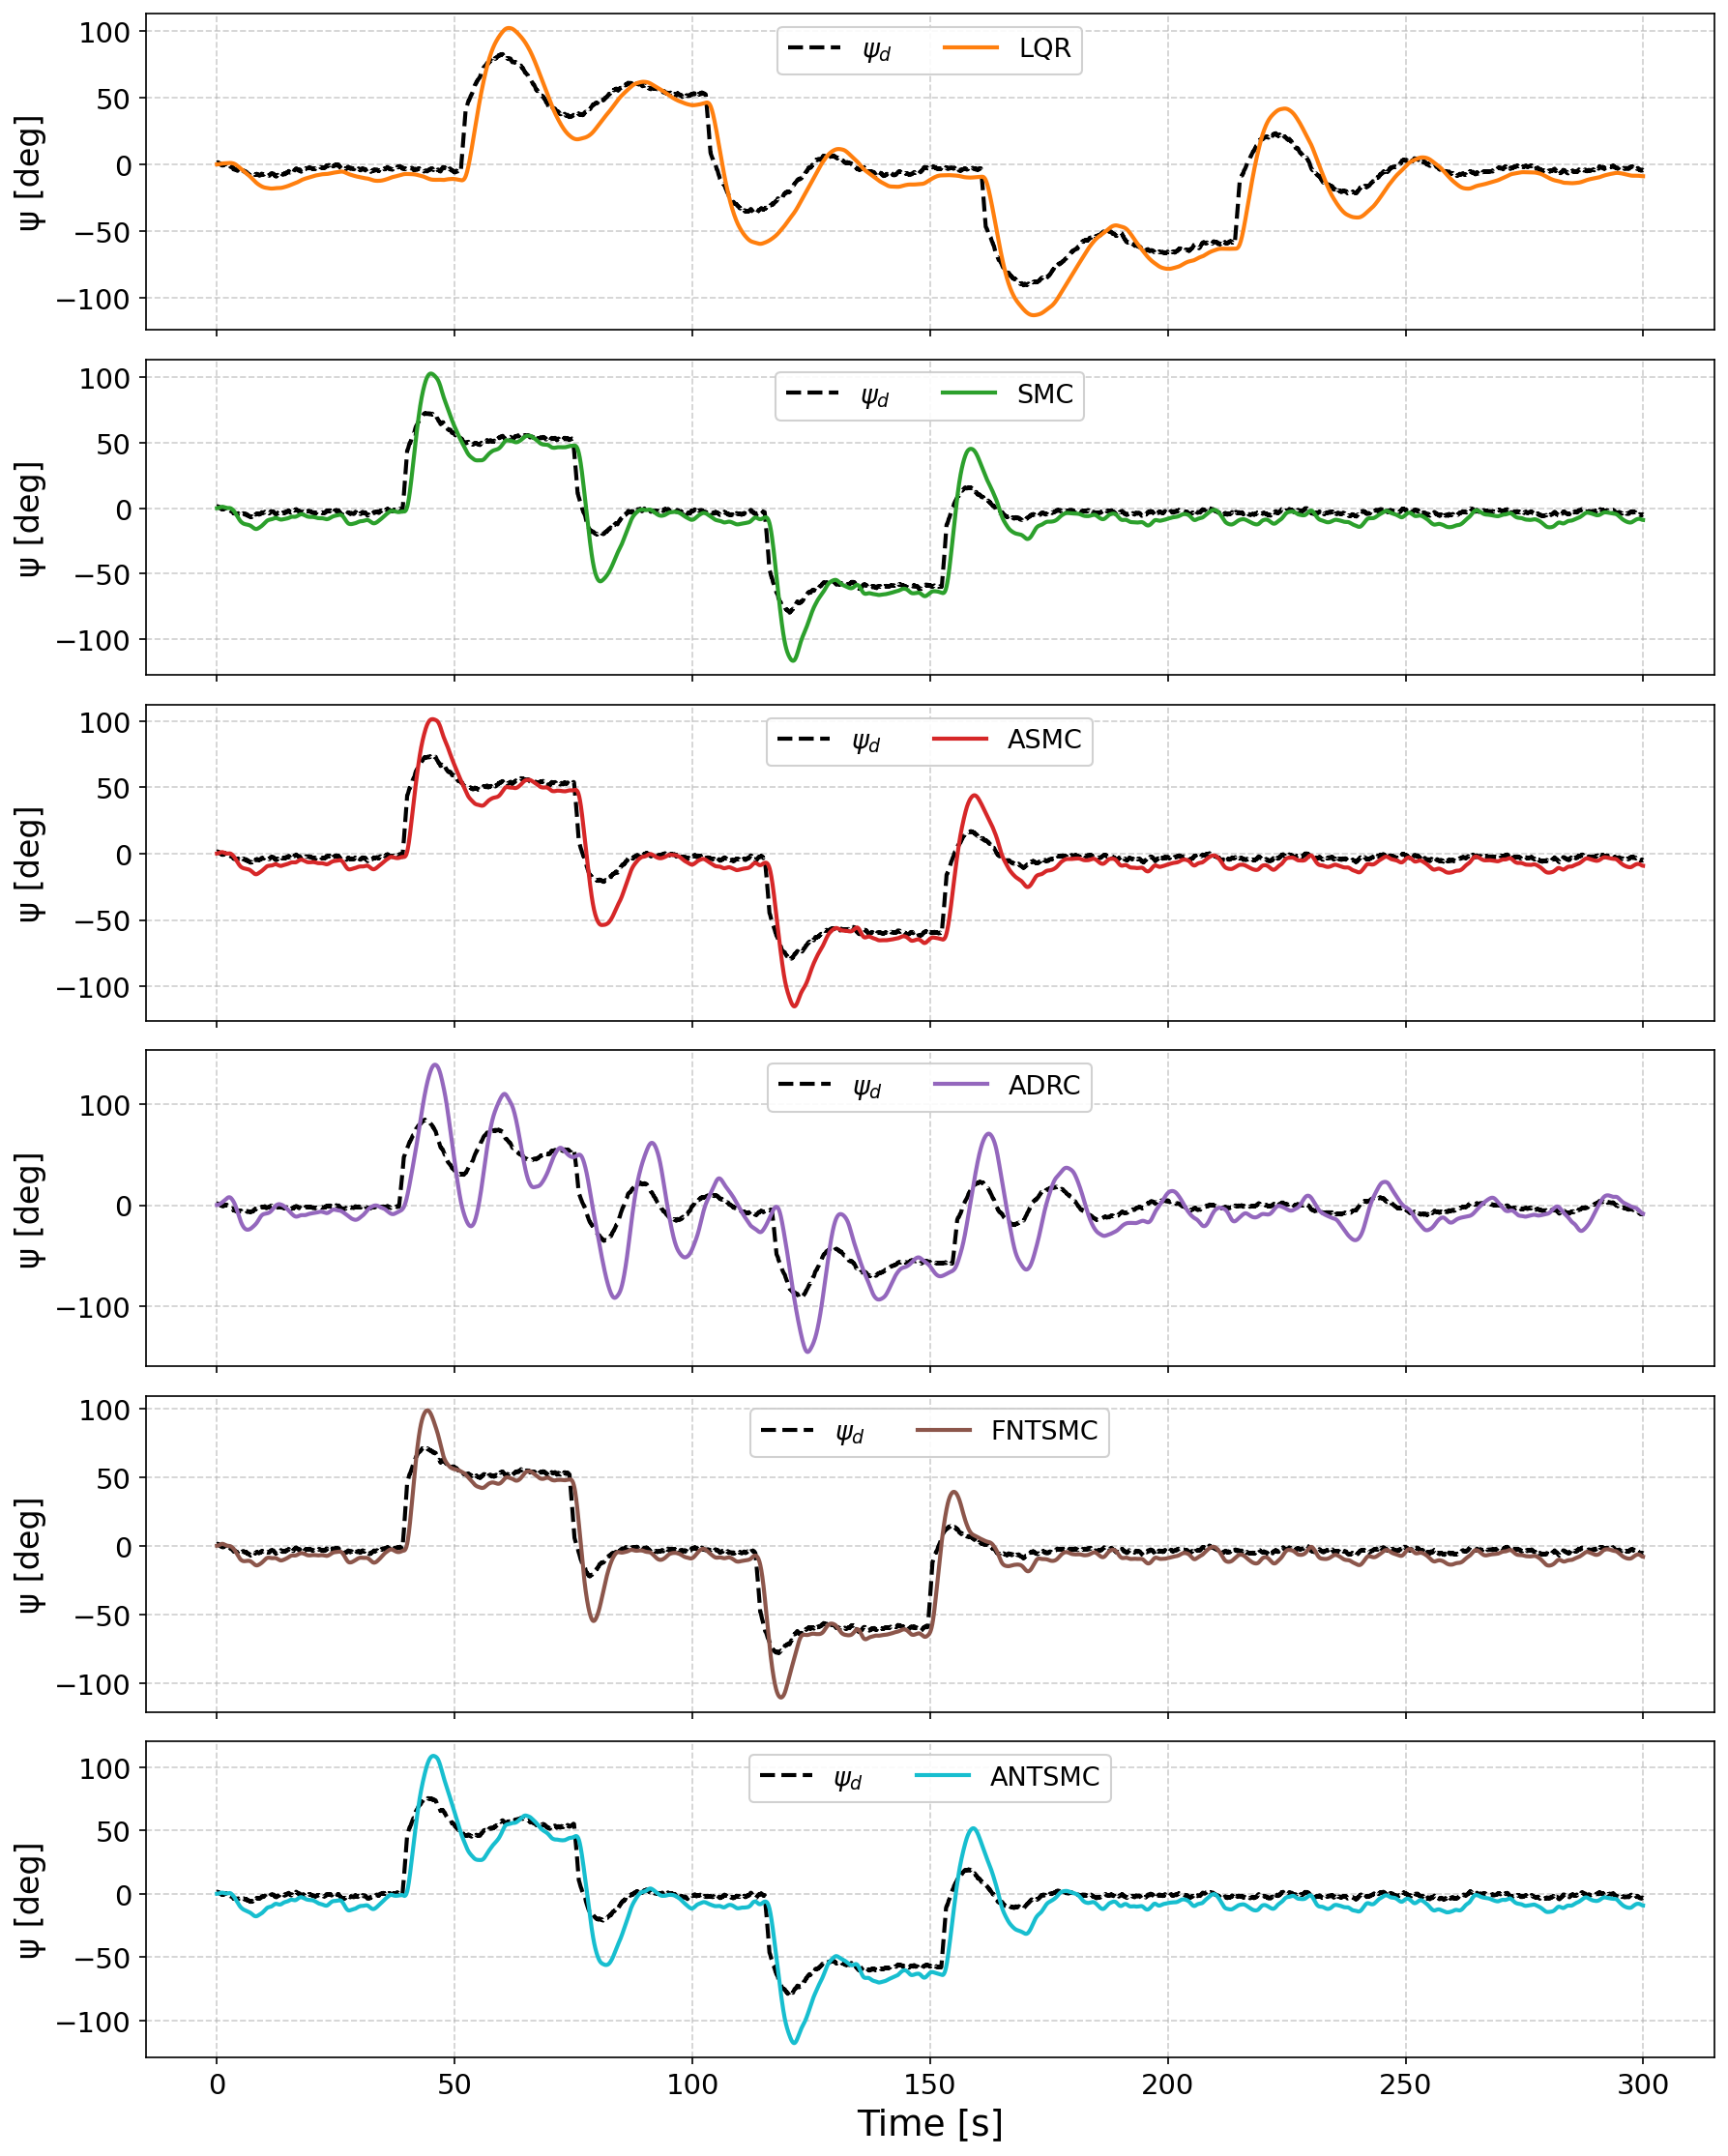
\includegraphics[width=\textwidth]{heading_custom_ss1.png}
  \caption{Custom path.}
  \label{fig:heading_custom_ss1}
\end{subfigure}\hfill
\begin{subfigure}[b]{0.48\textwidth}
  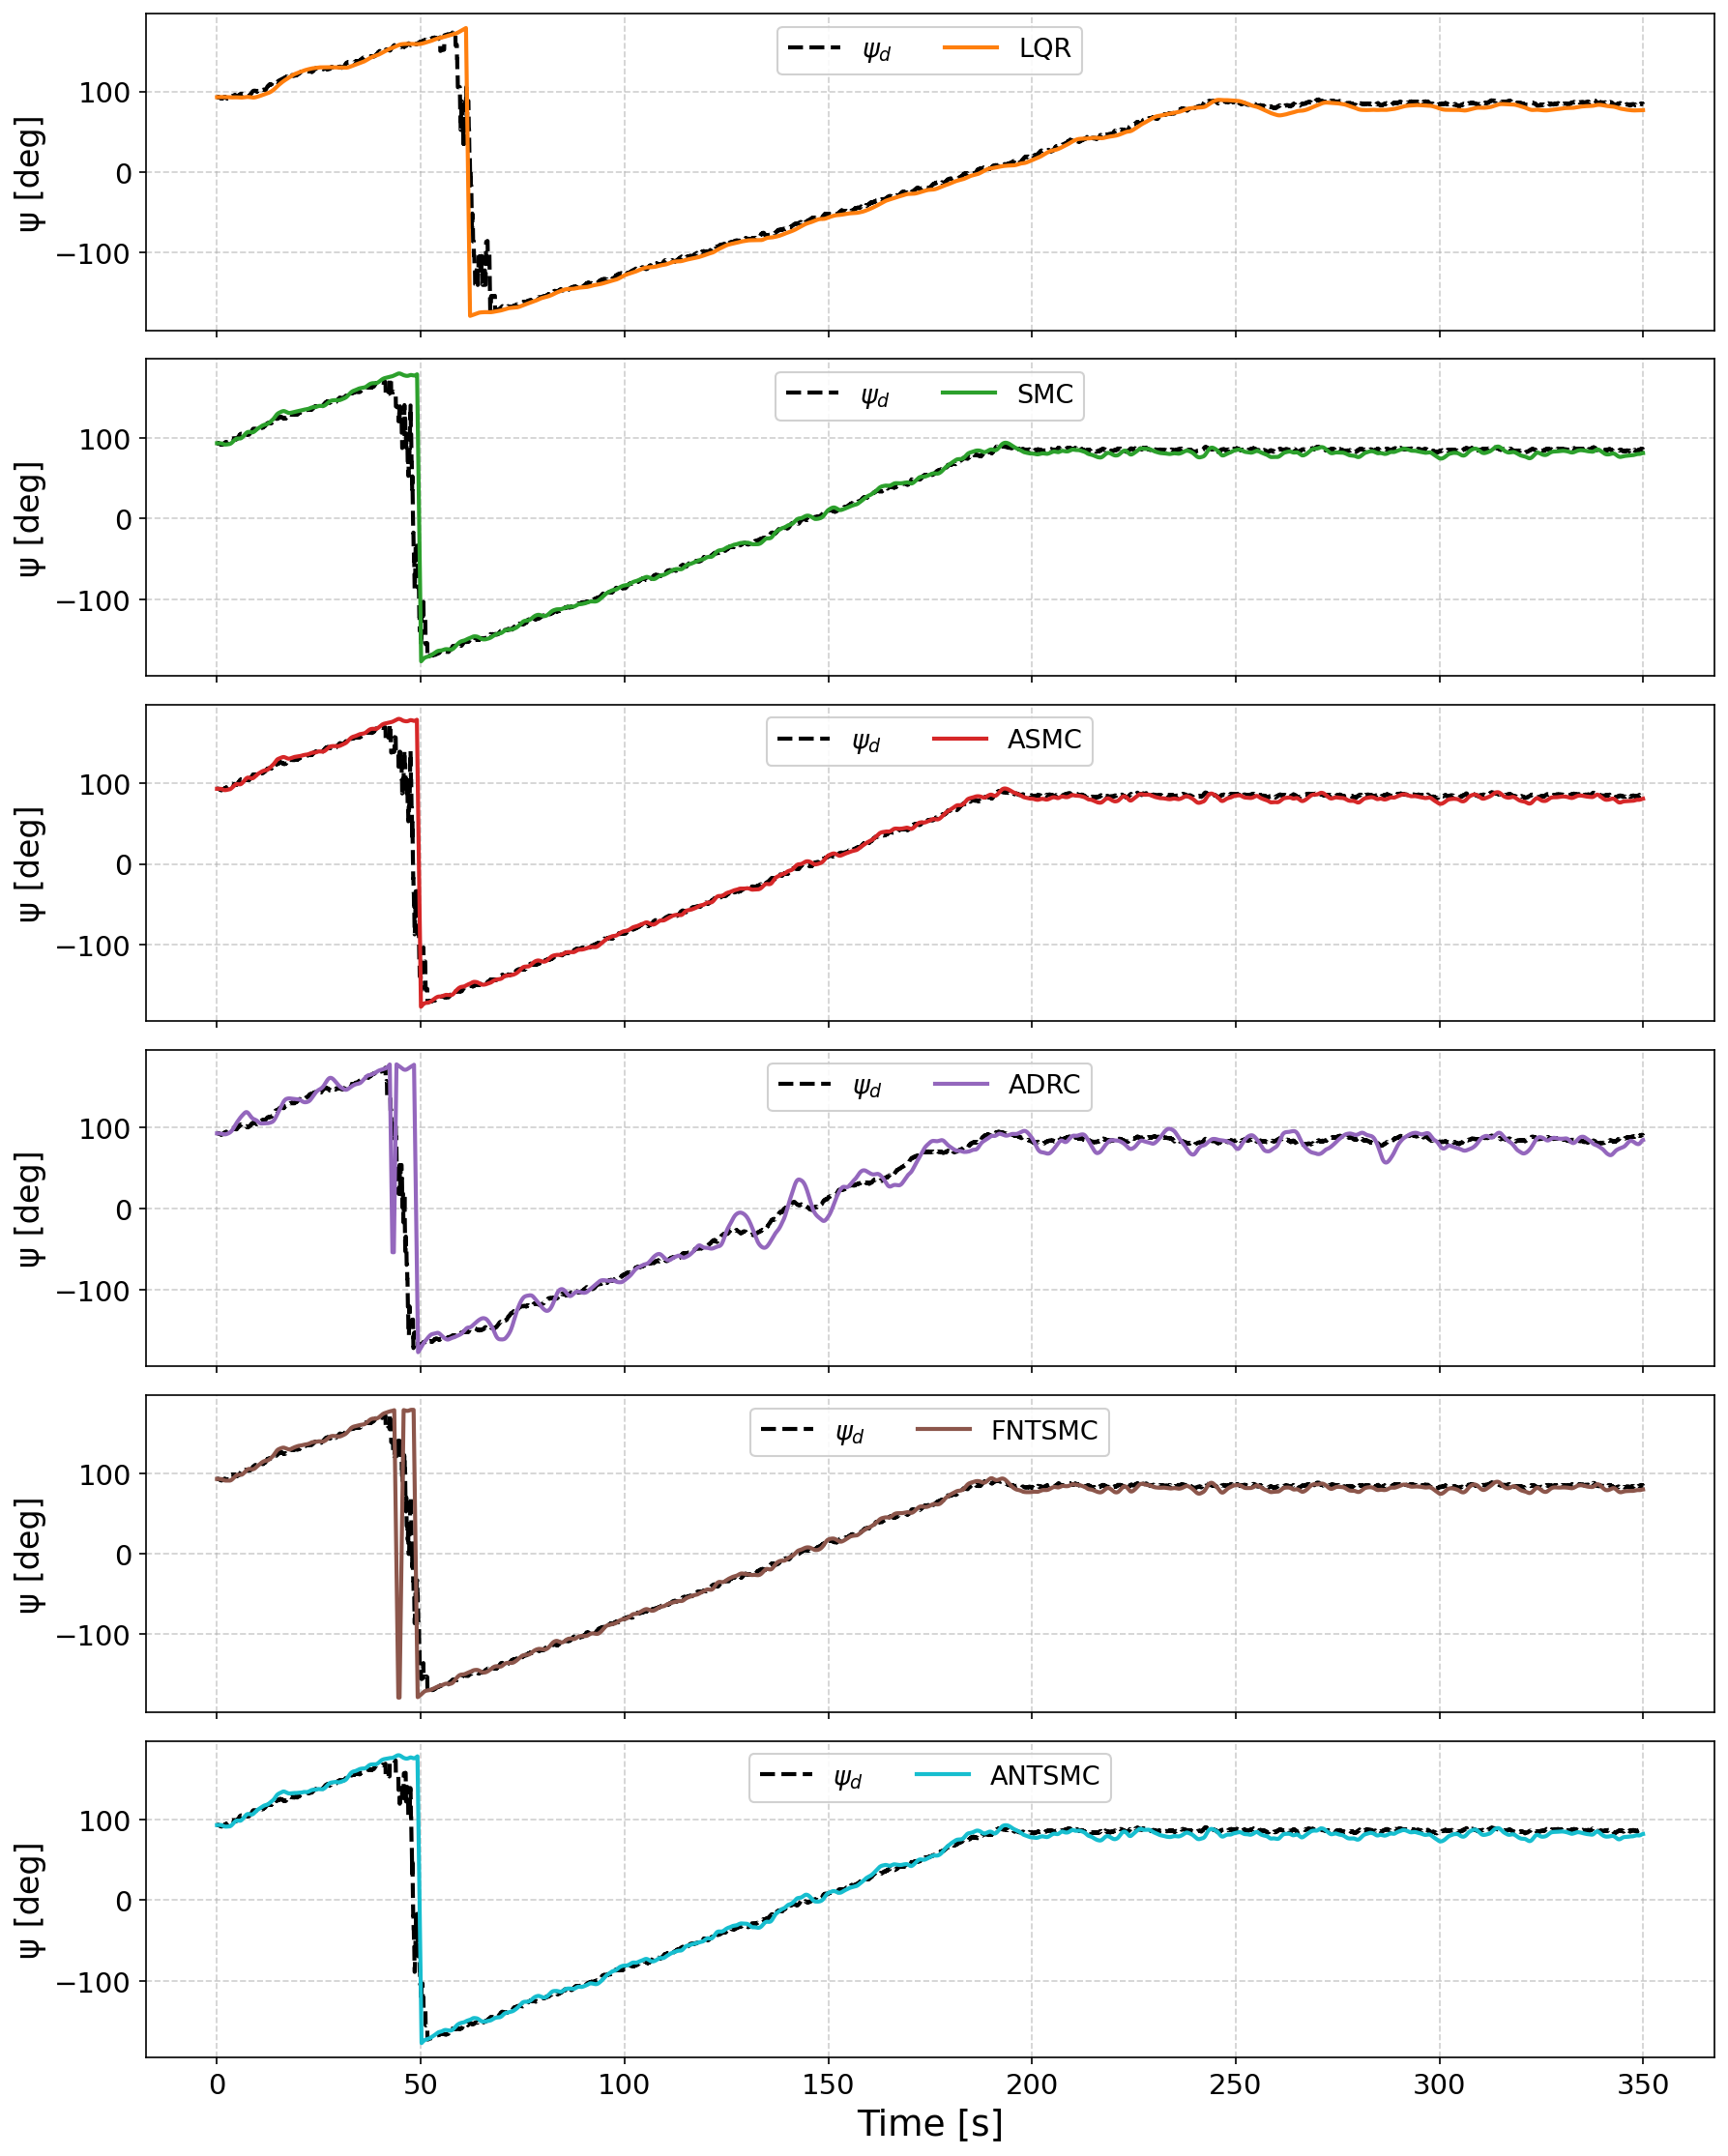
\includegraphics[width=\textwidth]{heading_circular_ss1.png}
  \caption{Circular path.}
\end{subfigure}\\[6pt]
\begin{subfigure}[b]{0.48\textwidth}
  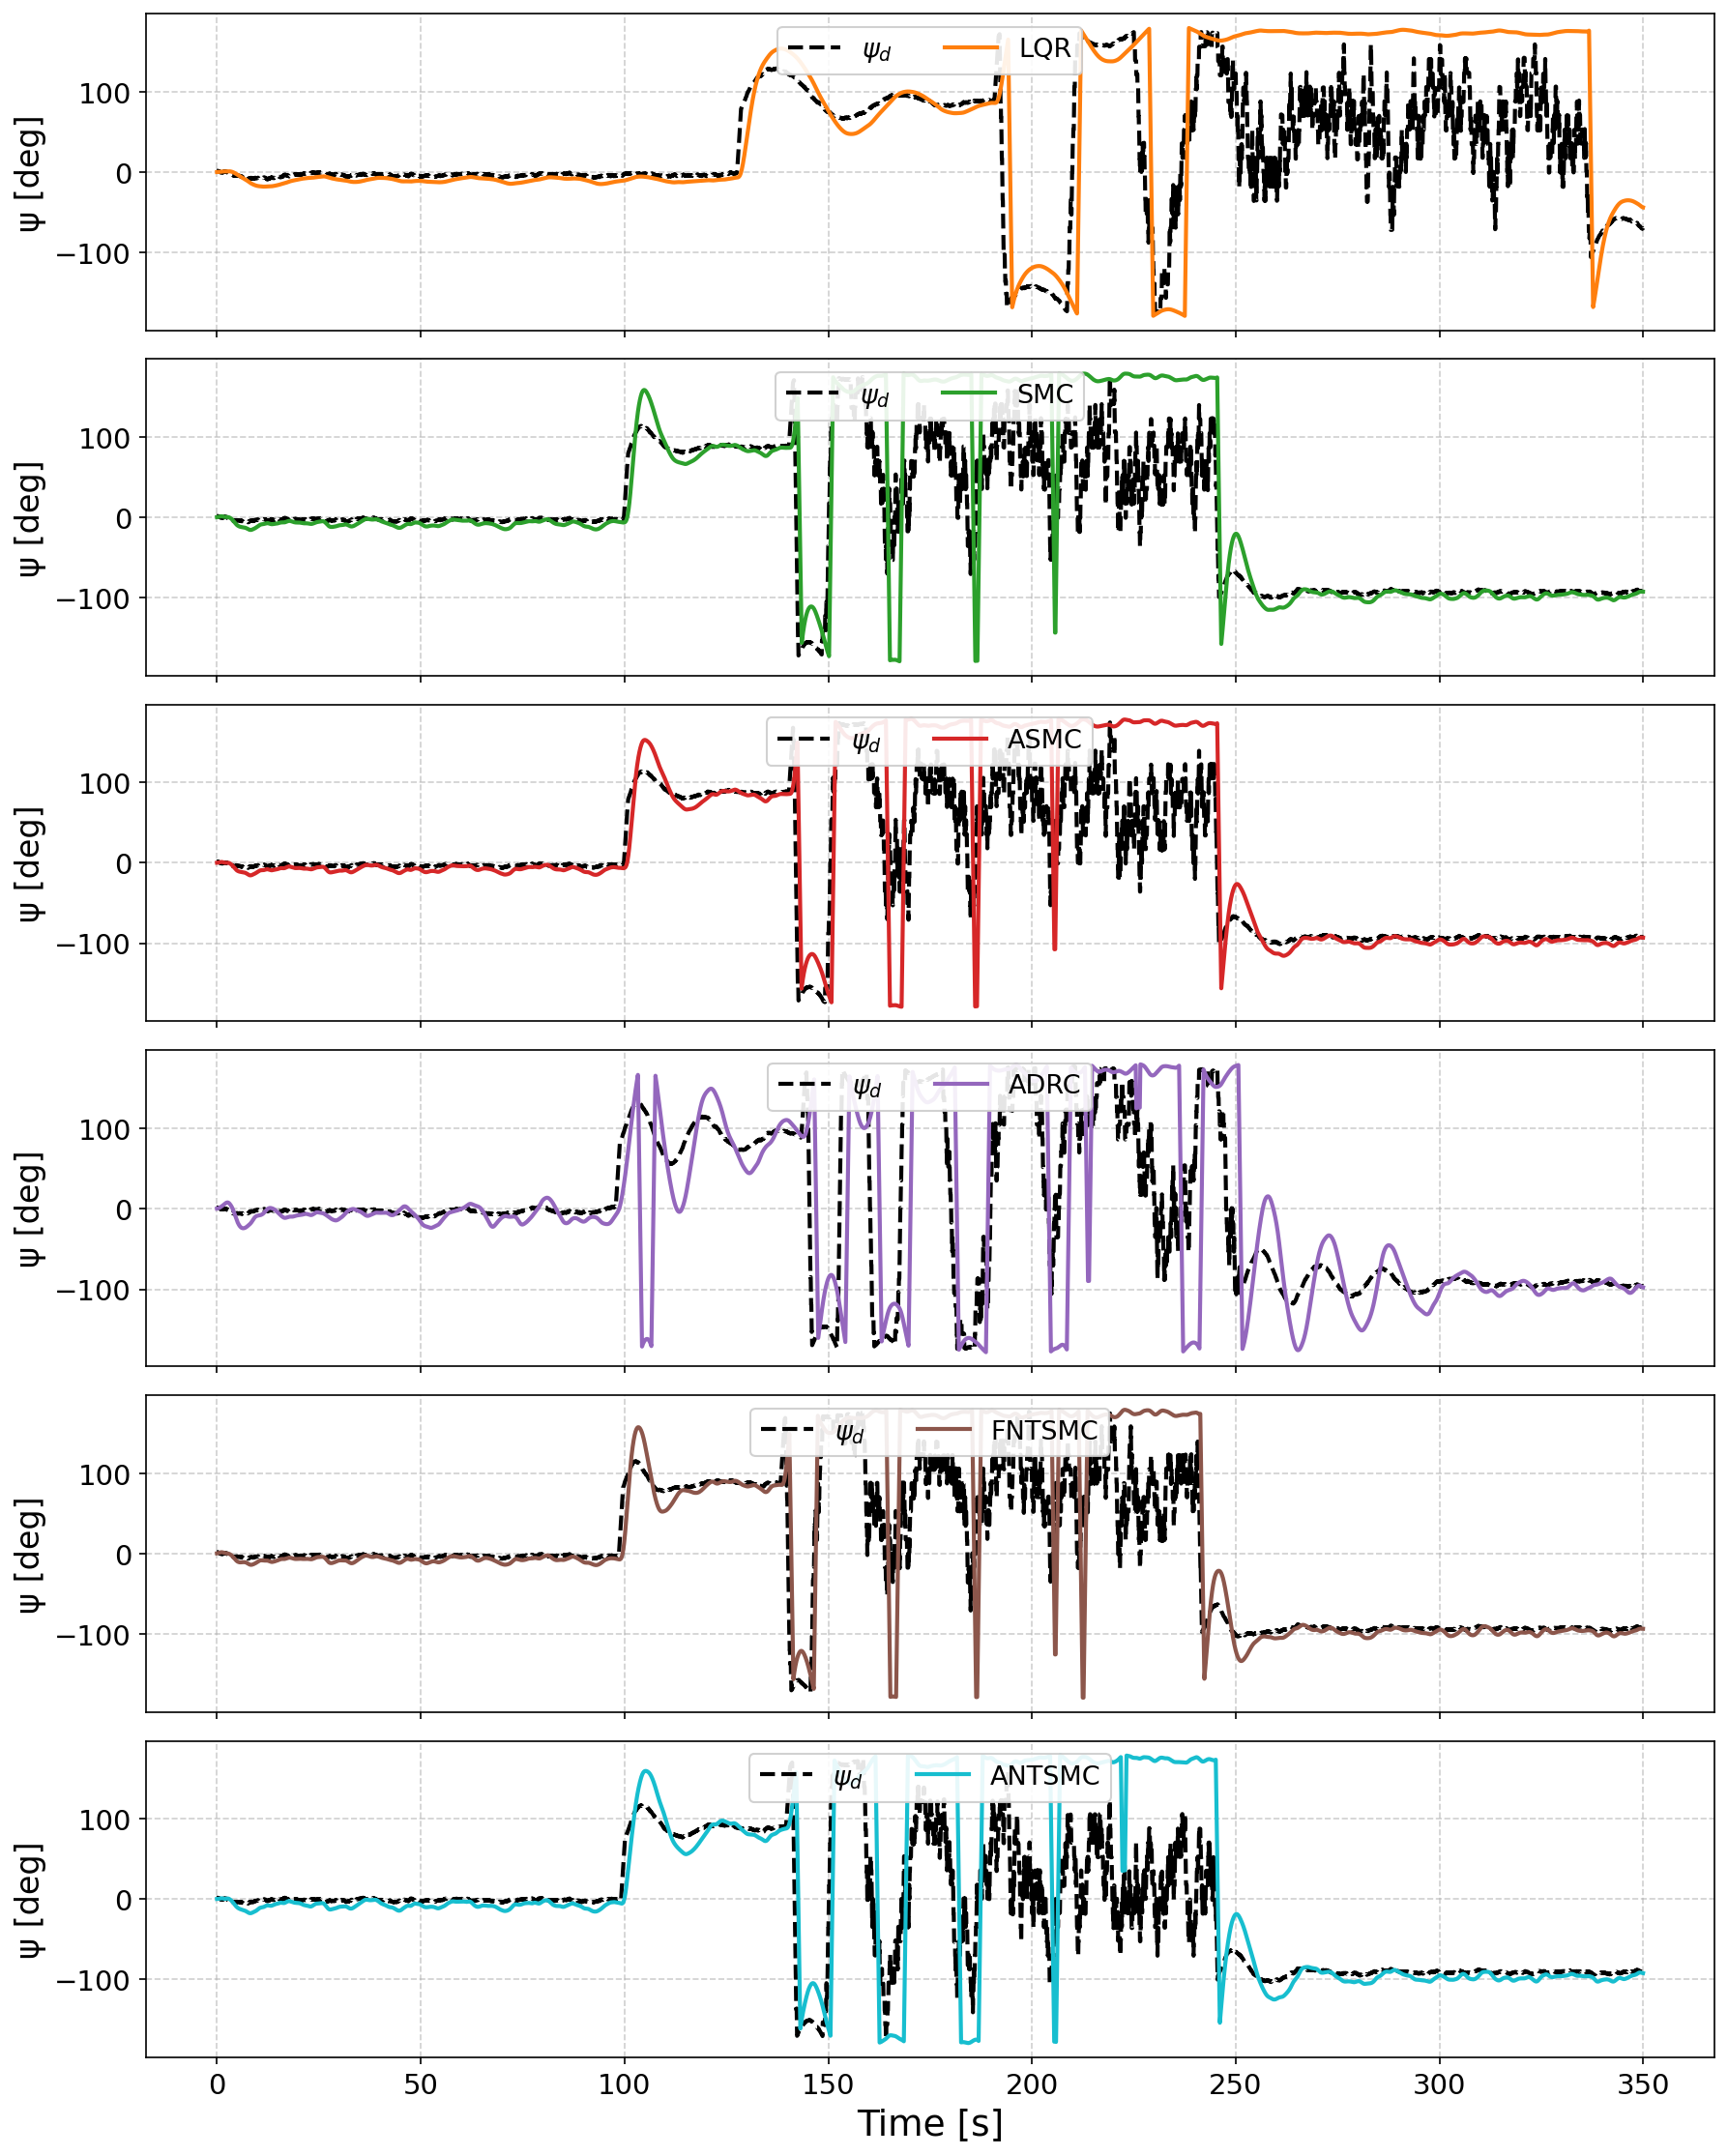
\includegraphics[width=\textwidth]{heading_rectangular_ss1.png}
  \caption{Rectangular path.}
\end{subfigure}\hfill
\begin{subfigure}[b]{0.48\textwidth}
  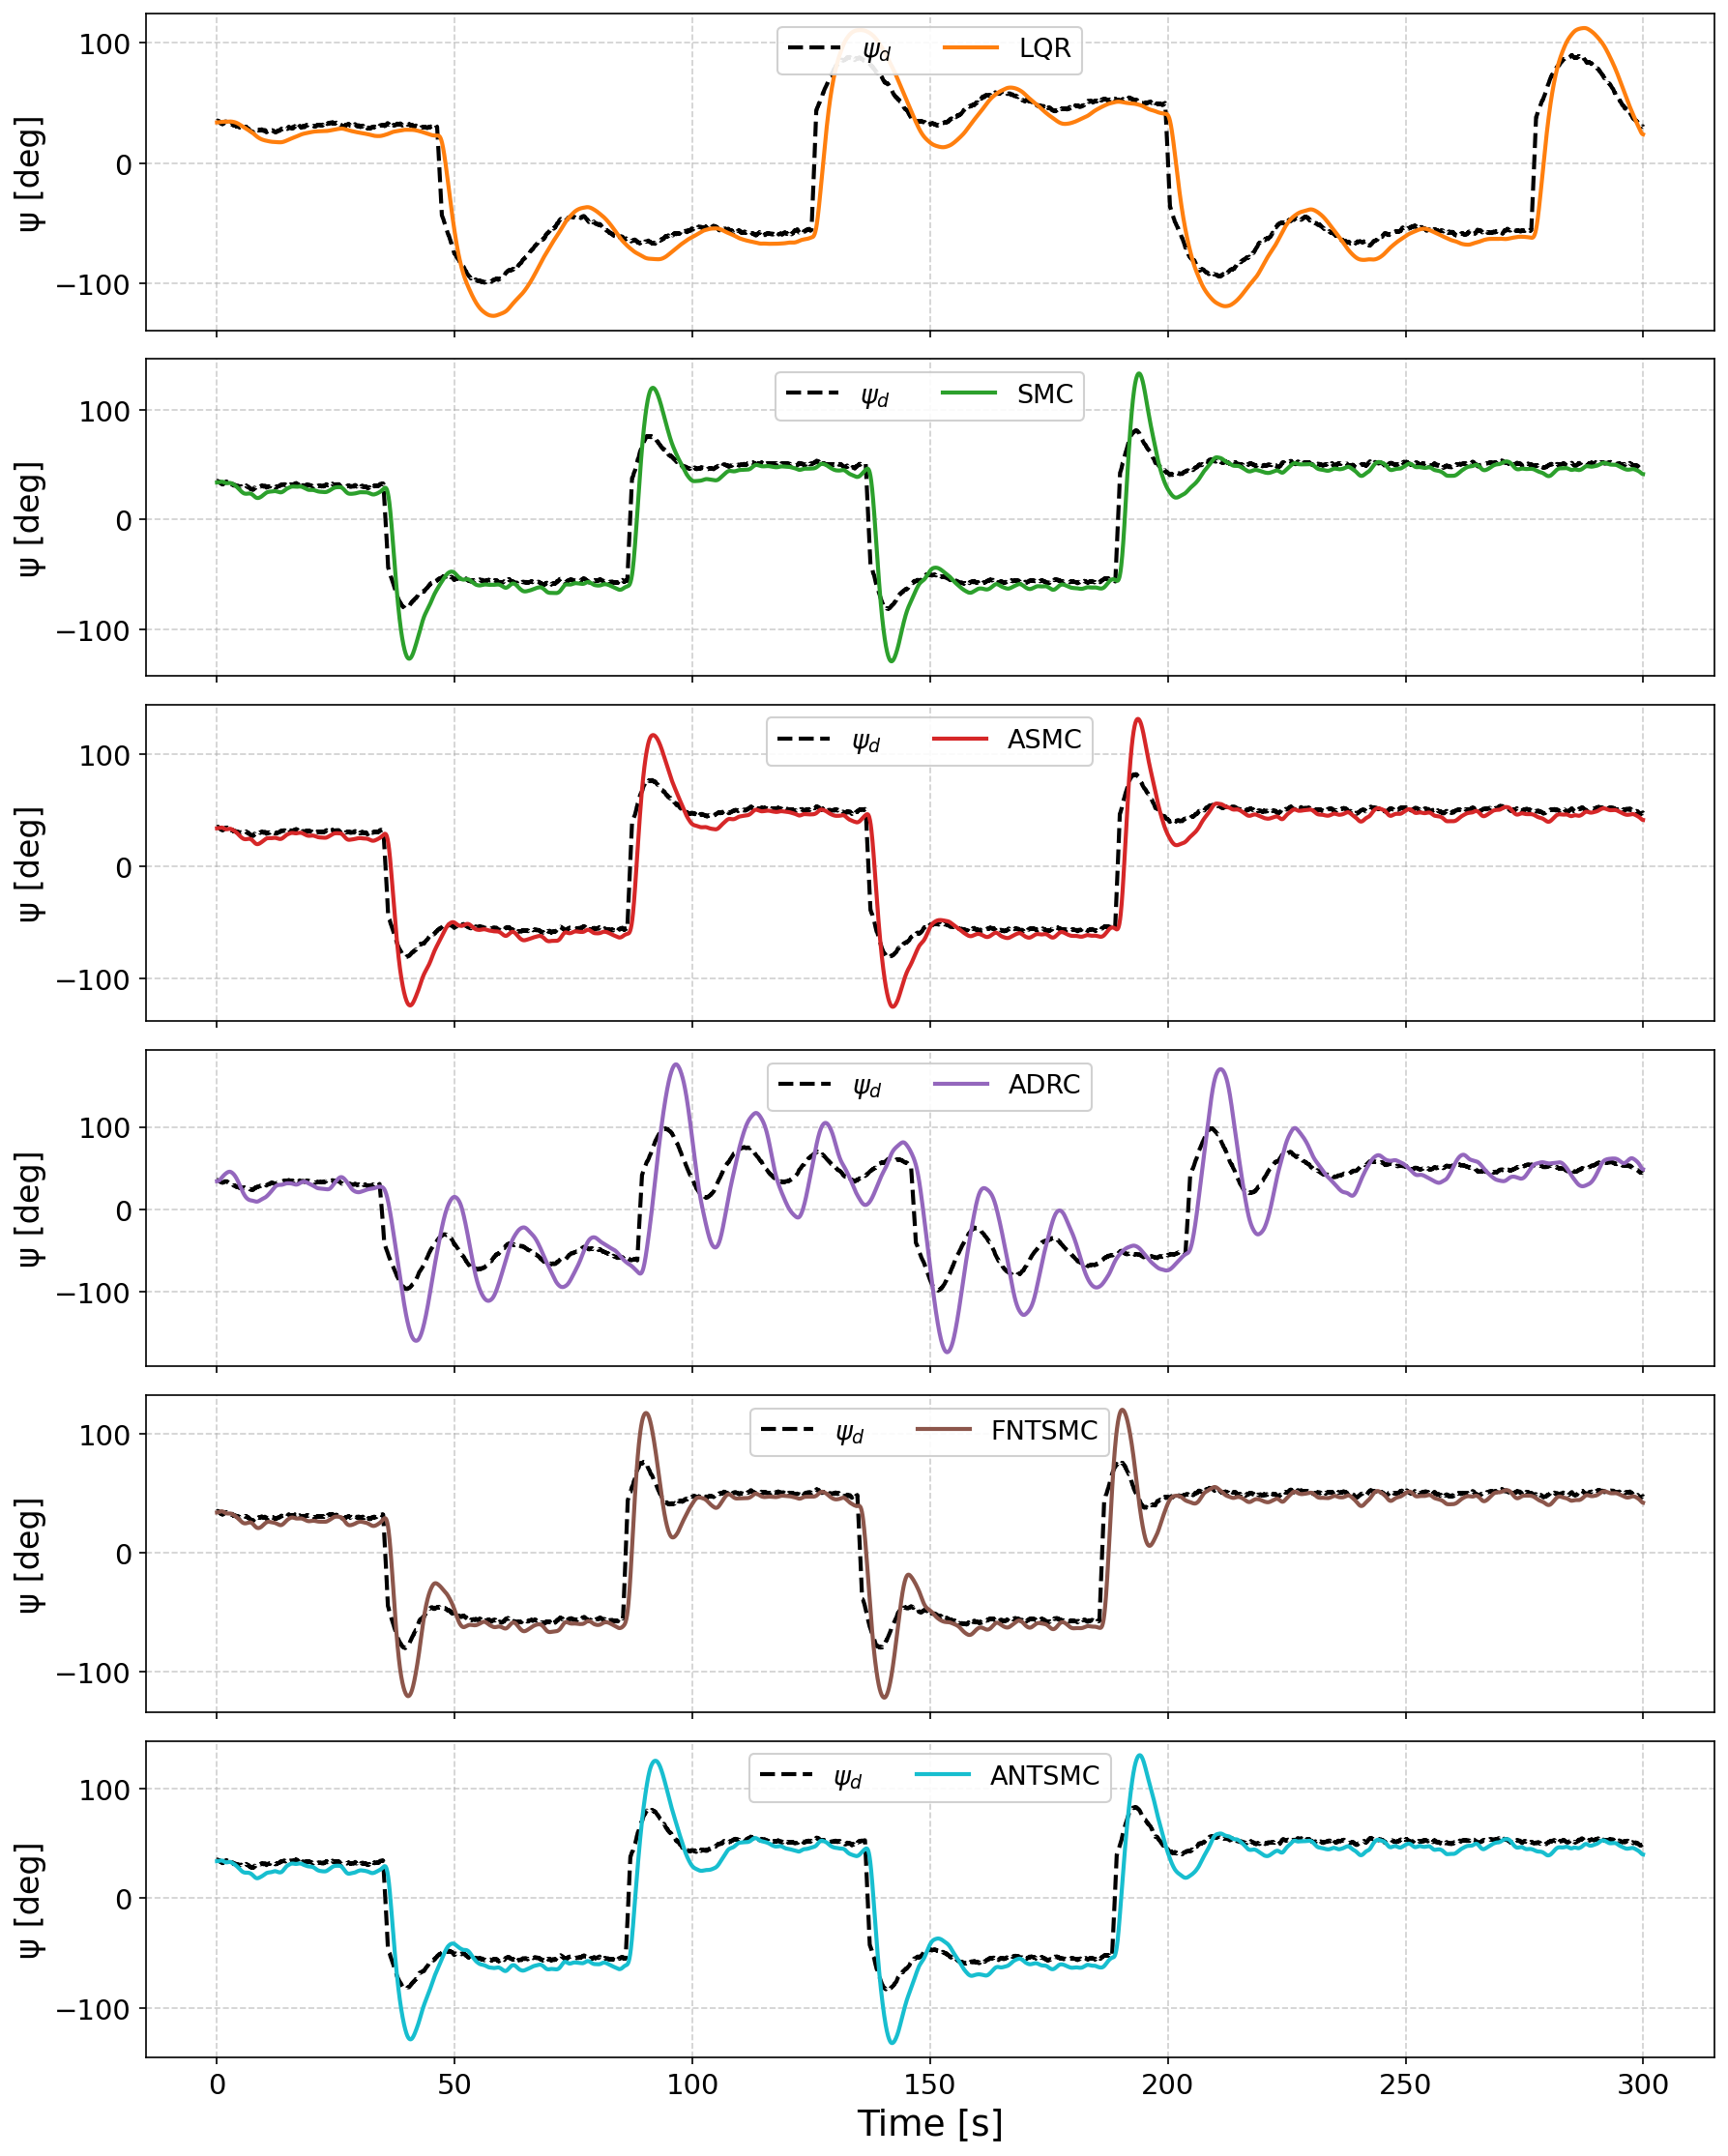
\includegraphics[width=\textwidth]{heading_zigzag_ss1.png}
  \caption{Zigzag path.}
\end{subfigure}
\caption{Heading tracking at Sea State~1 for all four paths. Each subplot shows an individual controller's heading response $\psi(t)$ against its desired heading $\psi_d(t)$, enabling direct assessment of heading tracking quality. ADRC shows ESO-induced heading lag at transitions; the sliding-mode controllers track closely.}
\label{fig:heading_ss1}
\end{figure*}

\subsubsection{Course Tracking at SS\,1}

Fig.~\ref{fig:course_ss1} provides a complementary view by overlaying the heading responses $\psi(t)$ of all controllers against the target course angle $\gamma$ on a single plot per path. This allows direct inter-controller comparison of how closely each follows the geometric path direction. SMC, FNTSMC, and ANTSMC track the course angle most faithfully, while LQR and ADRC exhibit larger deviations at path transitions.

\begin{figure*}[t]
\centering
\begin{subfigure}[b]{0.48\textwidth}
  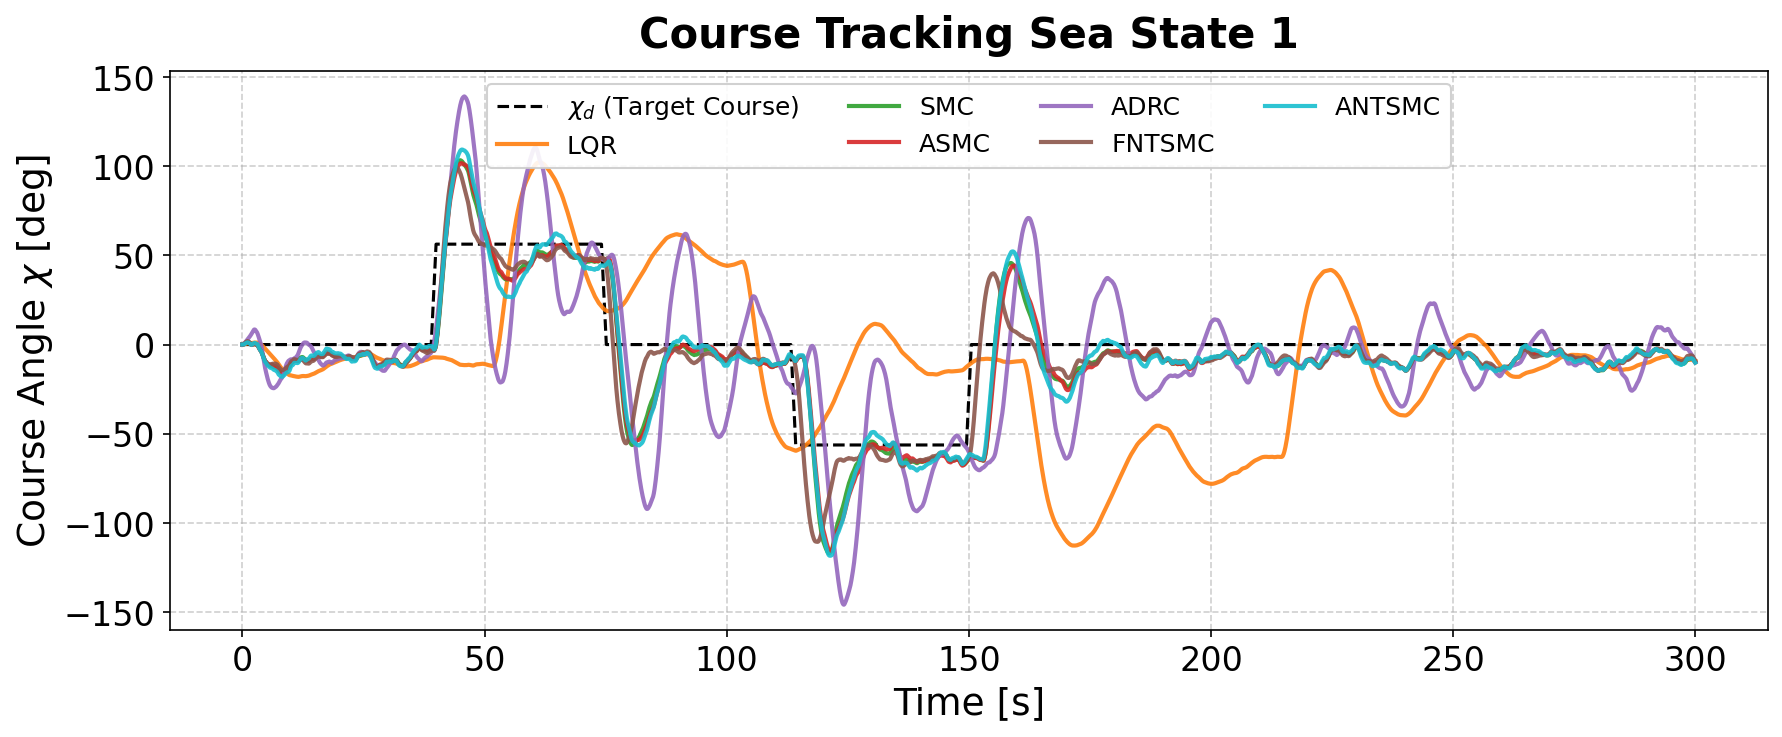
\includegraphics[width=\textwidth]{course_custom_ss1.png}
  \caption{Custom path.}
\end{subfigure}\hfill
\begin{subfigure}[b]{0.48\textwidth}
  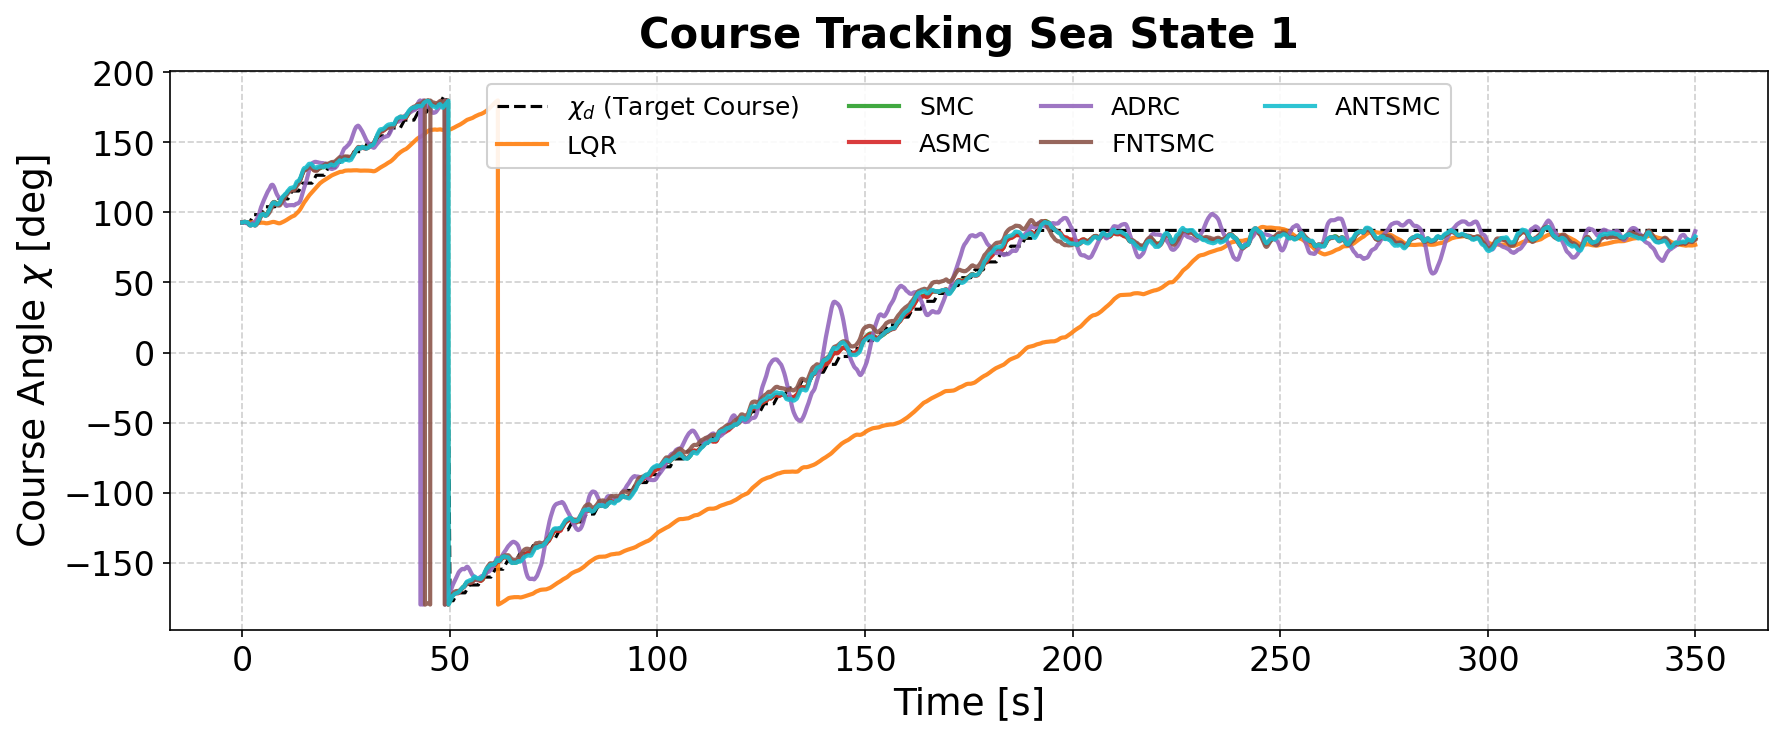
\includegraphics[width=\textwidth]{course_circular_ss1.png}
  \caption{Circular path.}
\end{subfigure}\\[6pt]
\begin{subfigure}[b]{0.48\textwidth}
  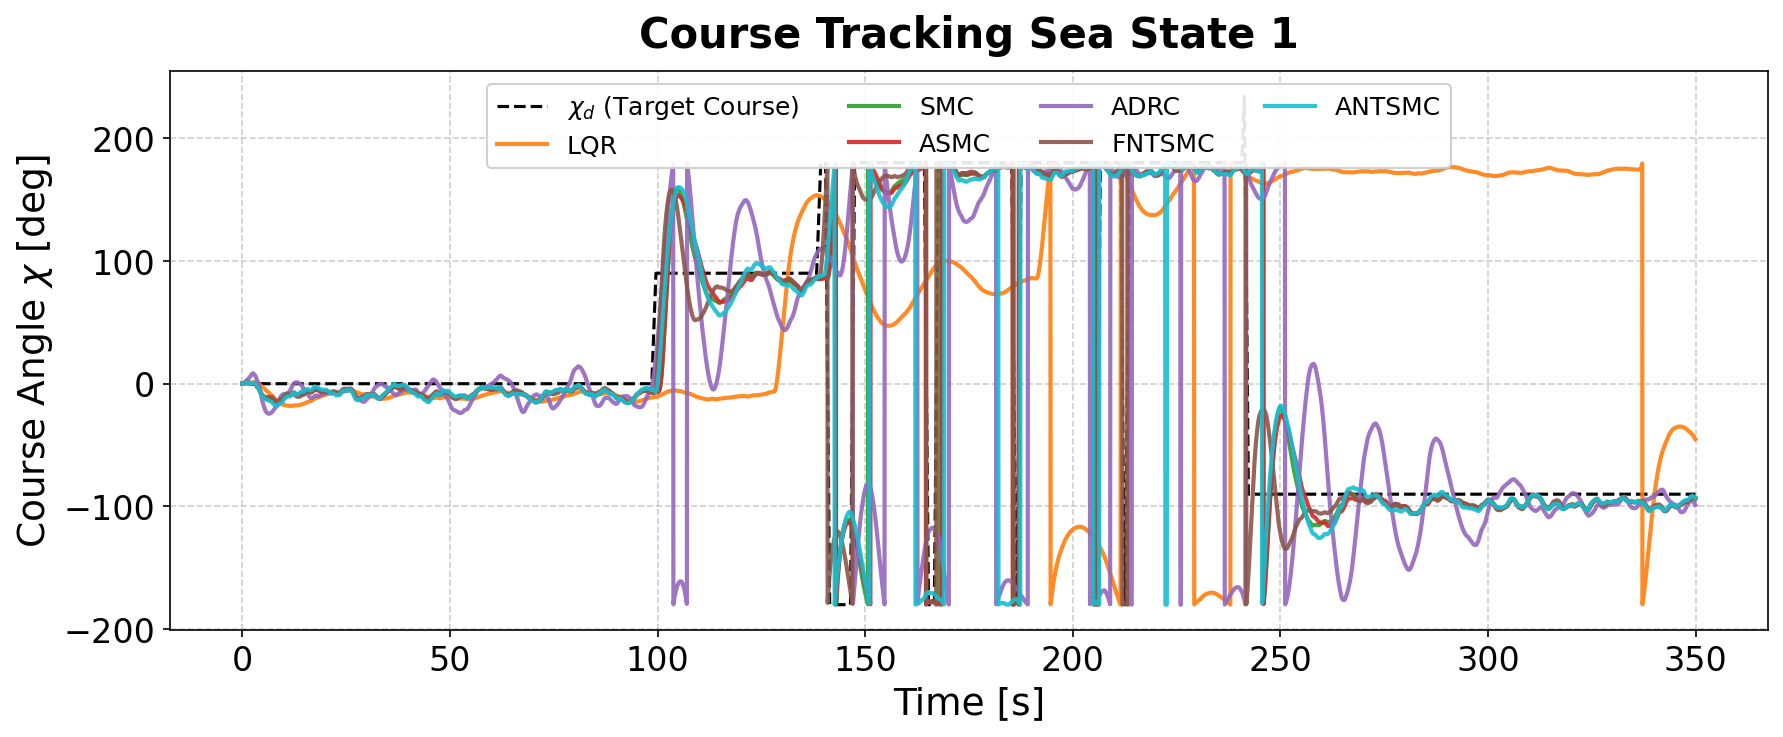
\includegraphics[width=\textwidth]{course_rectangular_ss1.png}
  \caption{Rectangular path.}
\end{subfigure}\hfill
\begin{subfigure}[b]{0.48\textwidth}
  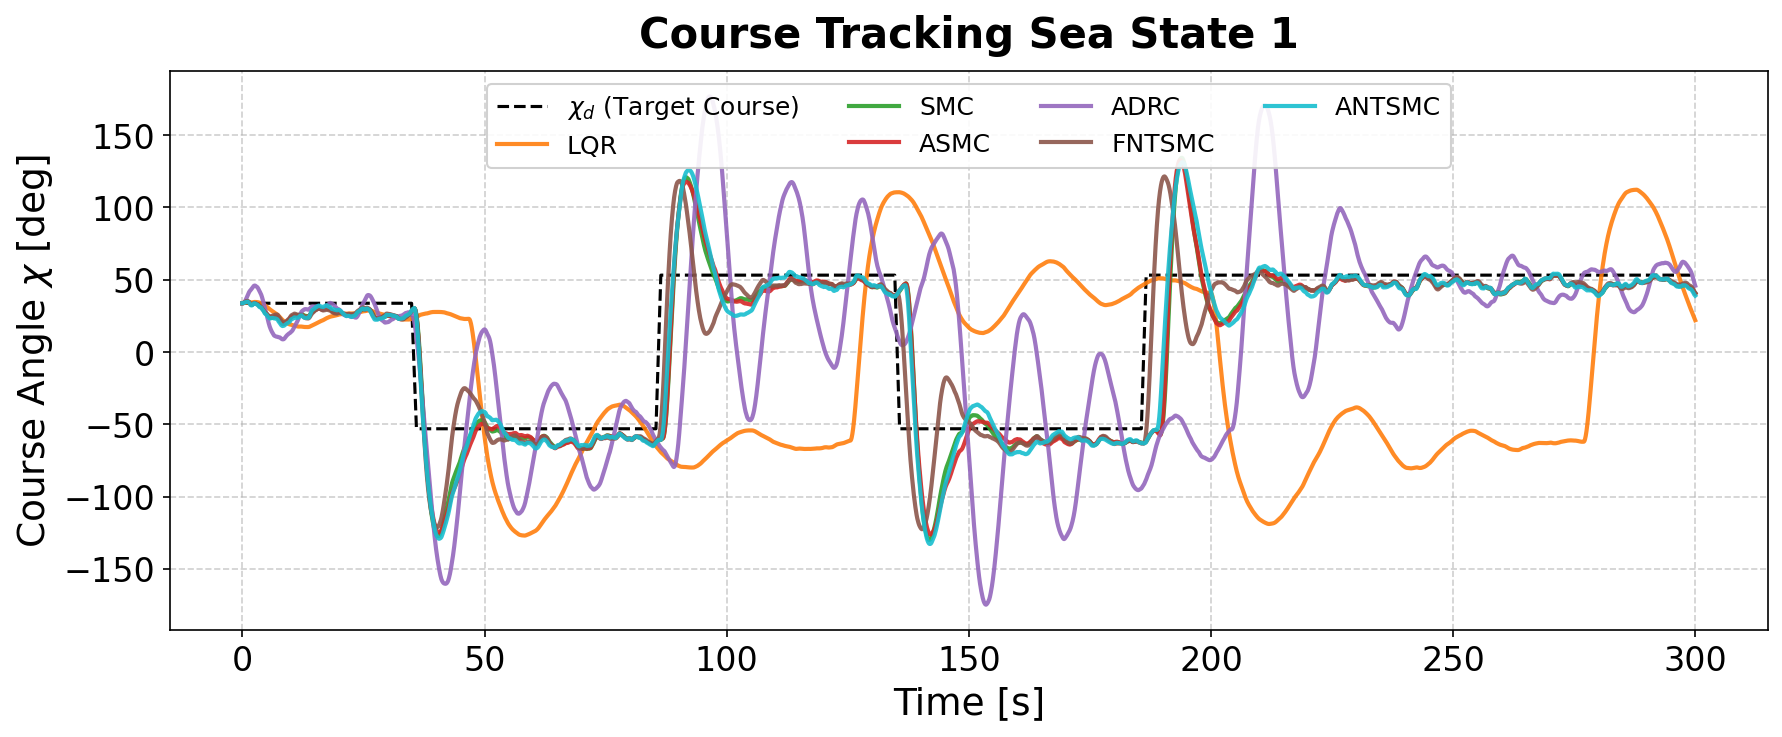
\includegraphics[width=\textwidth]{course_zigzag_ss1.png}
  \caption{Zigzag path.}
\end{subfigure}
\caption{Course tracking at Sea State~1 for all four paths. All controllers' heading responses are overlaid against the target course angle $\gamma$ (black dashed). SMC, FNTSMC, and ANTSMC follow the course most closely.}
\label{fig:course_ss1}
\end{figure*}

\subsubsection{Control Effort at SS\,1}

Fig.~\ref{fig:ctrl_ss1} shows the control effort signals. SMC-based controllers (SMC, ANTSMC) use higher yaw torques to achieve tighter tracking, while LQR uses less effort at the cost of larger errors.

\begin{figure*}[t]
\centering
\begin{subfigure}[b]{0.48\textwidth}
  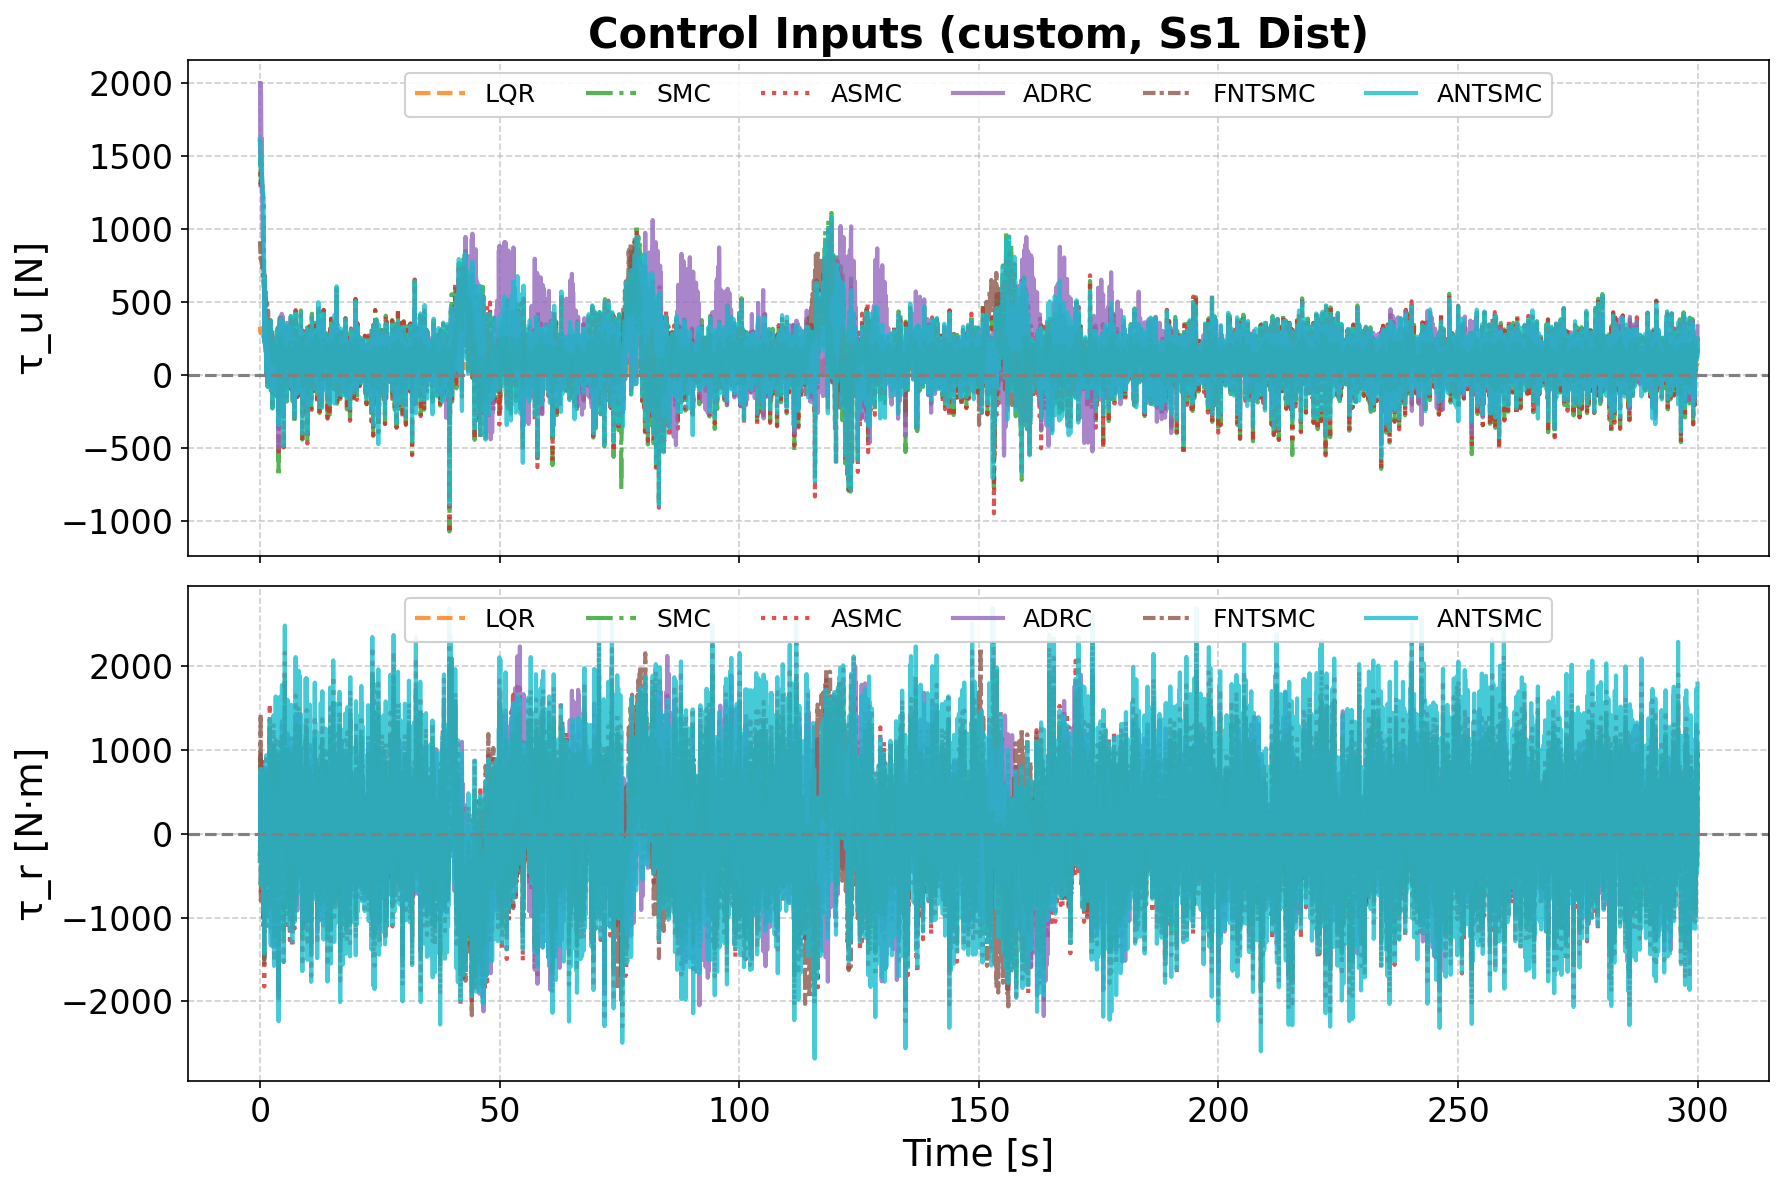
\includegraphics[width=\textwidth]{control_custom_ss1.png}
  \caption{Custom path.}
  \label{fig:ctrl_custom_ss1}
\end{subfigure}\hfill
\begin{subfigure}[b]{0.48\textwidth}
  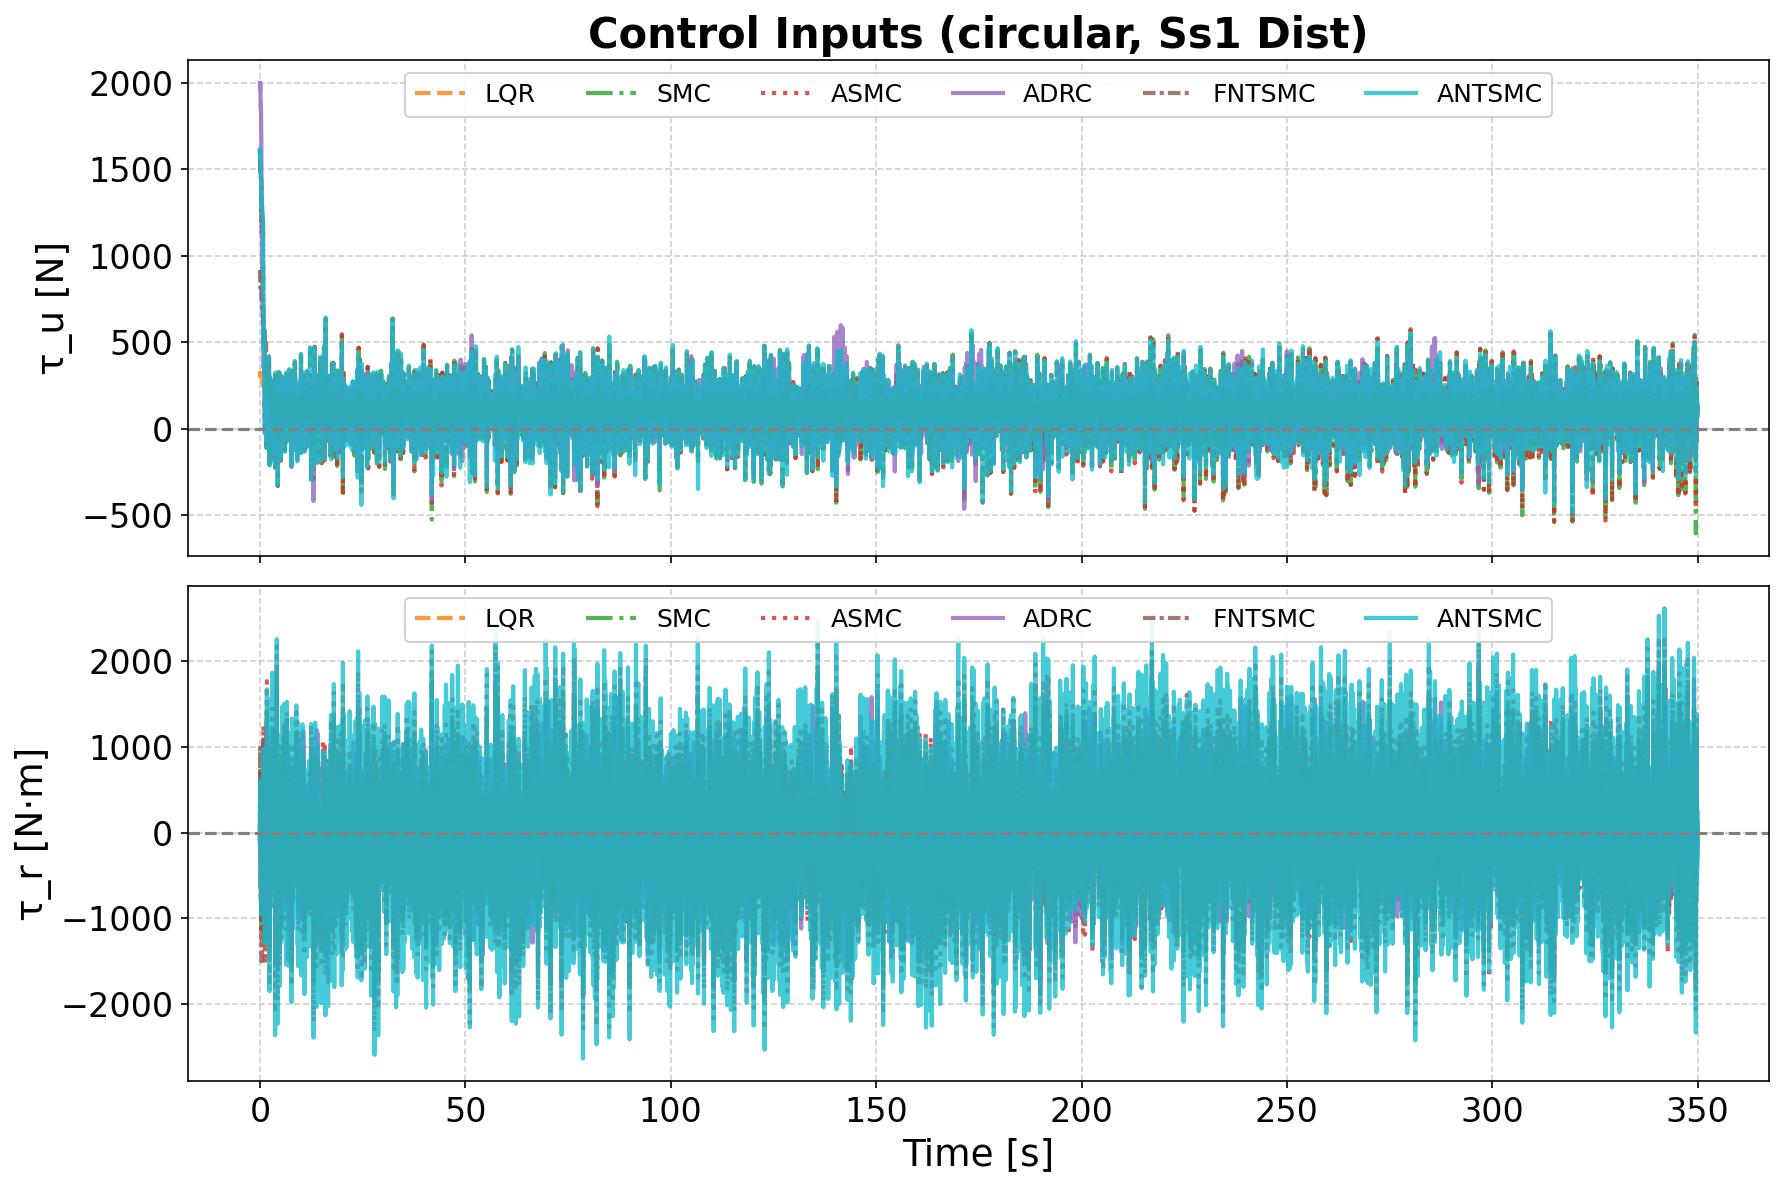
\includegraphics[width=\textwidth]{control_circular_ss1.png}
  \caption{Circular path.}
\end{subfigure}\\[6pt]
\begin{subfigure}[b]{0.48\textwidth}
  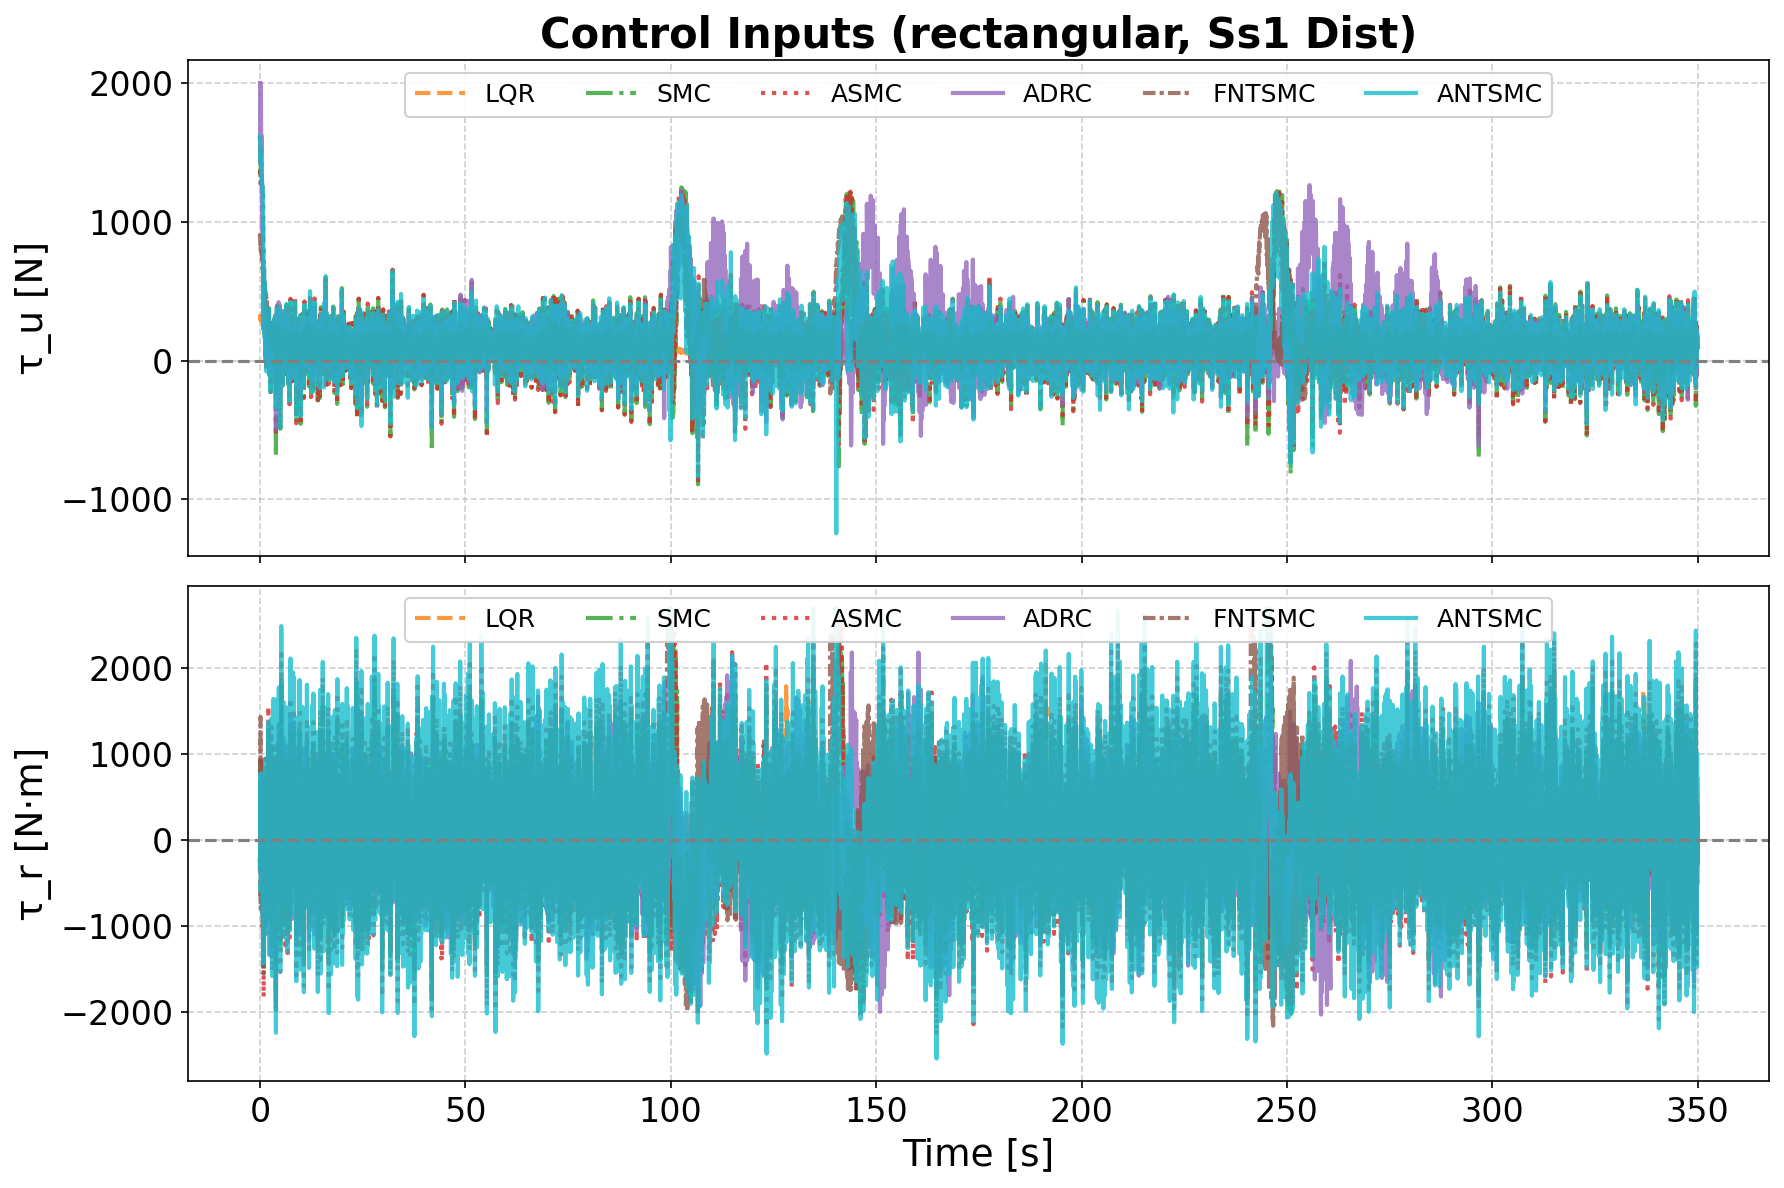
\includegraphics[width=\textwidth]{control_rectangular_ss1.png}
  \caption{Rectangular path.}
\end{subfigure}\hfill
\begin{subfigure}[b]{0.48\textwidth}
  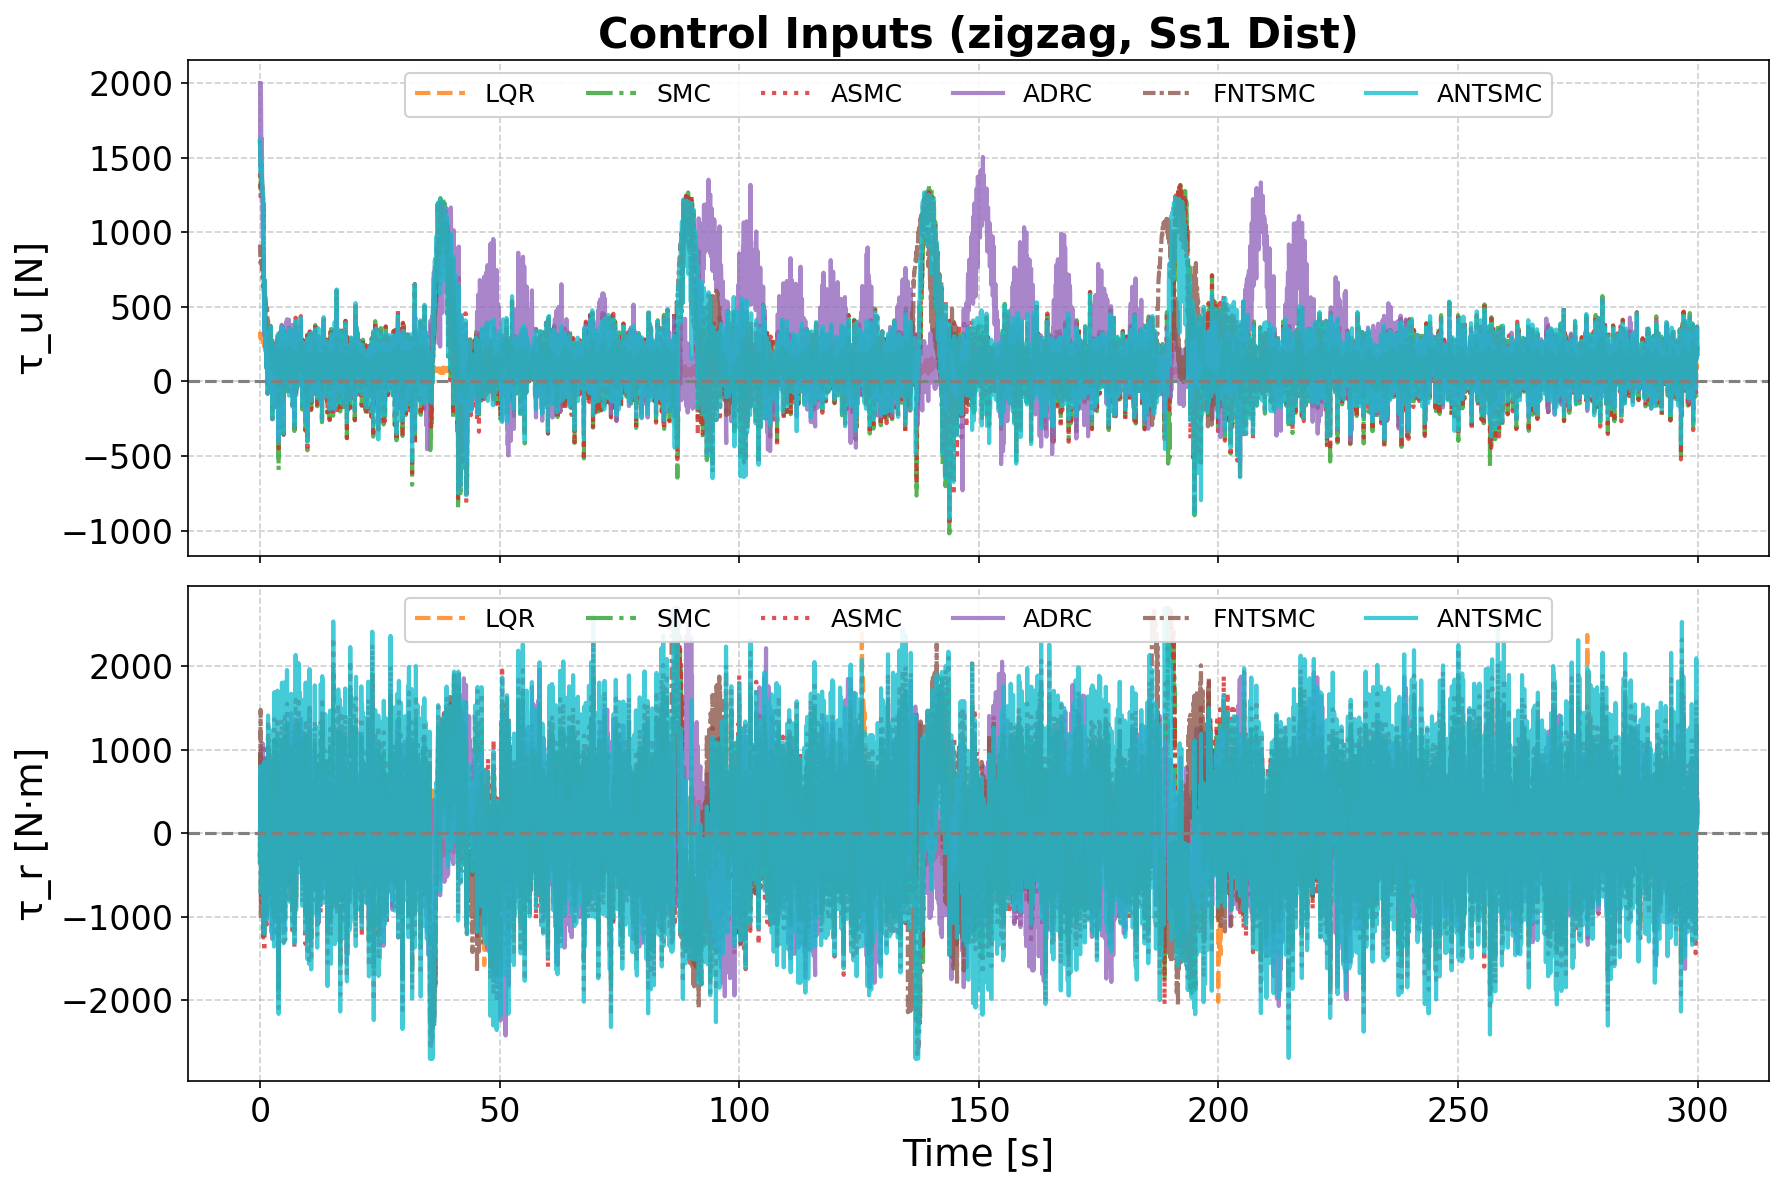
\includegraphics[width=\textwidth]{control_zigzag_ss1.png}
  \caption{Zigzag path.}
\end{subfigure}
\caption{Control effort ($\tau_u$, $\tau_r$) at Sea State~1 for all four paths. SMC-based controllers use higher yaw torques to maintain tighter tracking.}
\label{fig:ctrl_ss1}
\end{figure*}

\subsubsection{RMS Bar Chart --- SS\,1}

Fig.~\ref{fig:bar_ss1} provides an at-a-glance comparison of the RMS cross-track error for each controller grouped by path type at SS\,1.

\begin{figure}[t]
\centering
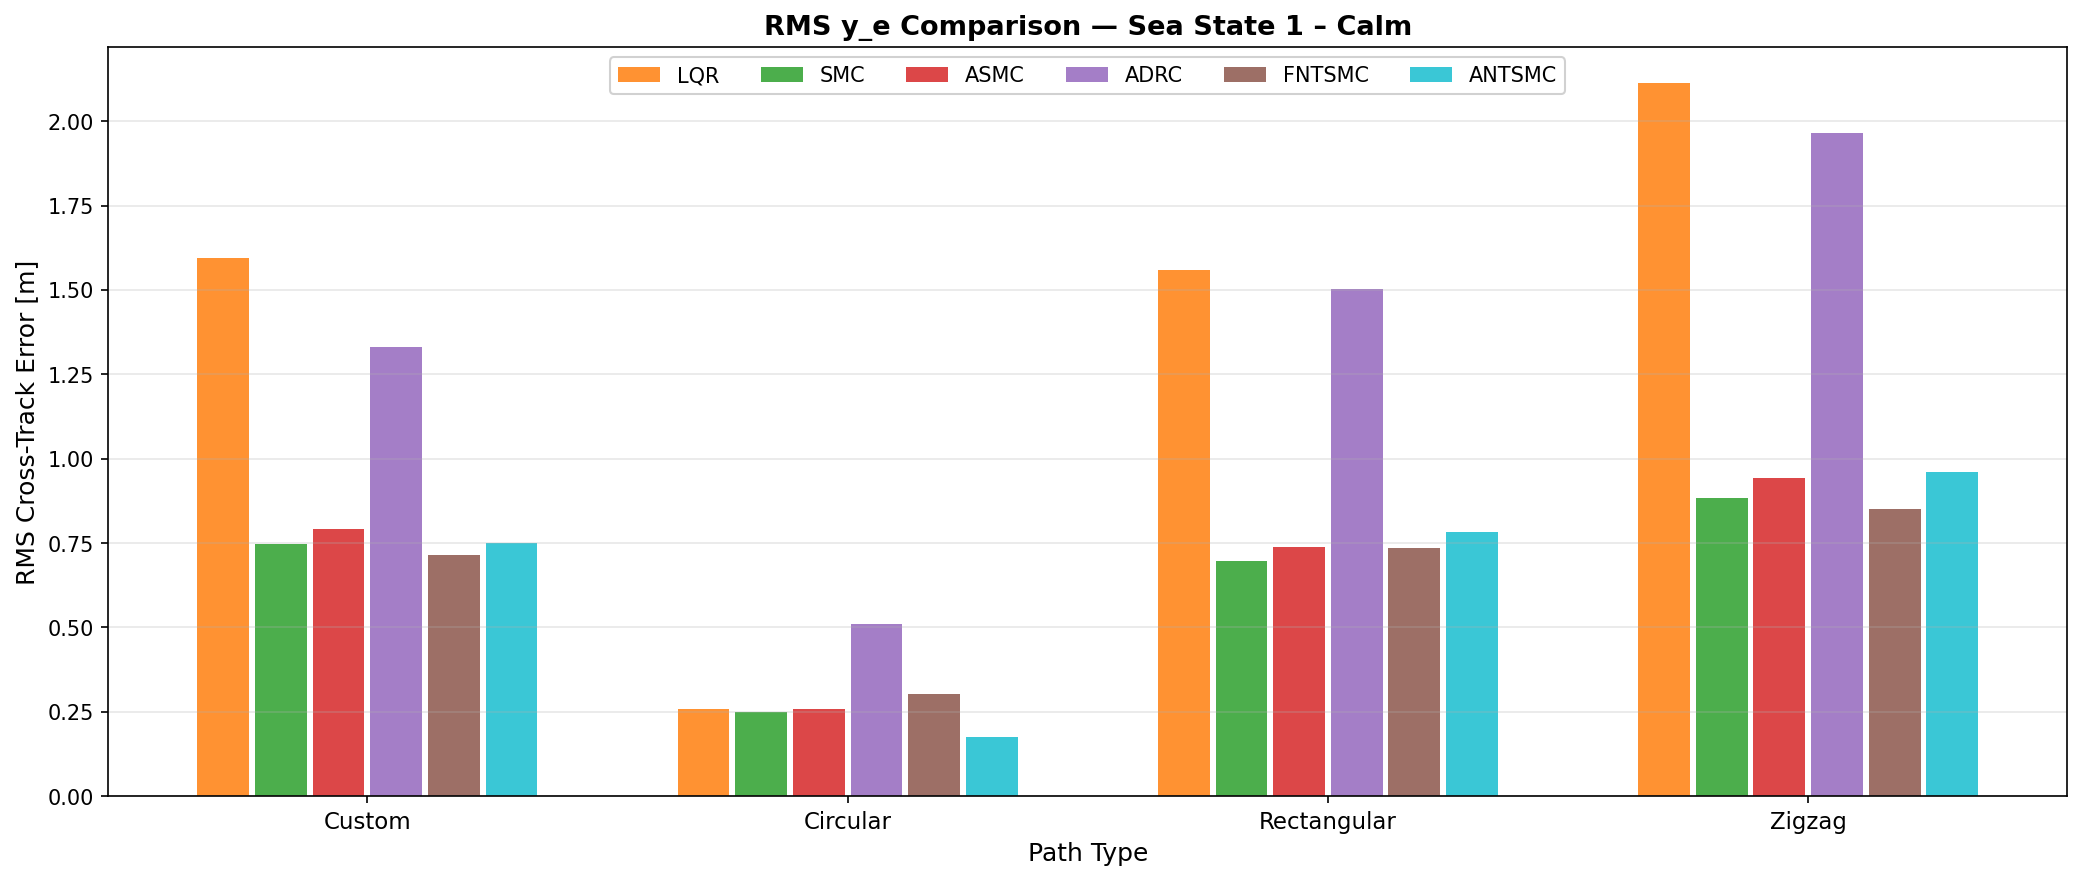
\includegraphics[width=\columnwidth]{bar_rms_ye_ss1.png}
\caption{RMS cross-track error bar chart at Sea State~1. SMC achieves the lowest bars across all paths, closely followed by FNTSMC and ANTSMC.}
\label{fig:bar_ss1}
\end{figure}


\subsection{Sea State 2 --- Smooth ($\alpha_s = 0.35$)}

Under moderate disturbances (Table~\ref{tab:ss2}), \textbf{ANTSMC takes the lead} with RMS $y_e = 1.226$~m---a 10.2\% improvement over SMC (1.364~m) and 31.3\% over ADRC (1.782~m). The adaptive switching gain begins increasing ($k_{s,r} \approx 0.7$--$0.9$), providing disturbance rejection that exceeds SMC's fixed gain, while the terminal surface maintains tight tracking once the sliding surface is reached. Notably, ASMC (1.412~m) slightly outperforms FNTSMC (1.491~m), suggesting that the FTDO's observer lag begins to penalise FNTSMC under growing disturbances.

\textbf{Ranking (SS\,2):} \#1 ANTSMC, \#2 SMC, \#3 ASMC, \#4 FNTSMC, \#5 ADRC, \#6 LQR.

\begin{table}[t]
\centering
\caption{Sea State 2 (Smooth) --- cross-path average steady-state performance. Best values in \textbf{bold}.}
\label{tab:ss2}
\begin{tabular}{lccccc}
\toprule
Controller & RMS $y_e$ [m] & Max $|y_e|$ [m] & RMS $\tau_u$ [N] & RMS $\tau_r$ [N\,m] & Energy \\
\midrule
LQR & 2.617 & 6.940 & 47.1 & 278.8 & 18\,828 \\
SMC & 1.364 & 3.644 & 295.1 & 687.8 & 140\,487 \\
ASMC & 1.412 & 3.793 & 291.9 & 792.2 & 141\,991 \\
ADRC & 1.782 & 5.238 & 261.4 & 674.5 & 124\,852 \\
FNTSMC & 1.491 & 3.576 & 185.7 & 697.7 & 86\,444 \\
\textbf{ANTSMC} & \textbf{1.226} & \textbf{3.769} & 271.4 & 801.5 & 131\,298 \\
\bottomrule
\end{tabular}
\end{table}

\subsubsection{Trajectory Tracking at SS\,2}

Fig.~\ref{fig:traj_ss2} compares trajectory tracking at SS\,2. The performance gap between controllers widens visibly compared to SS\,1. ANTSMC and SMC maintain tight tracking on all paths, while LQR exhibits significantly larger deviations, especially at corners and reversals. FNTSMC performs well on smooth segments but shows slight overshoots at sharp corners due to FTDO lag.

\begin{figure*}[t]
\centering
\begin{subfigure}[b]{0.48\textwidth}
  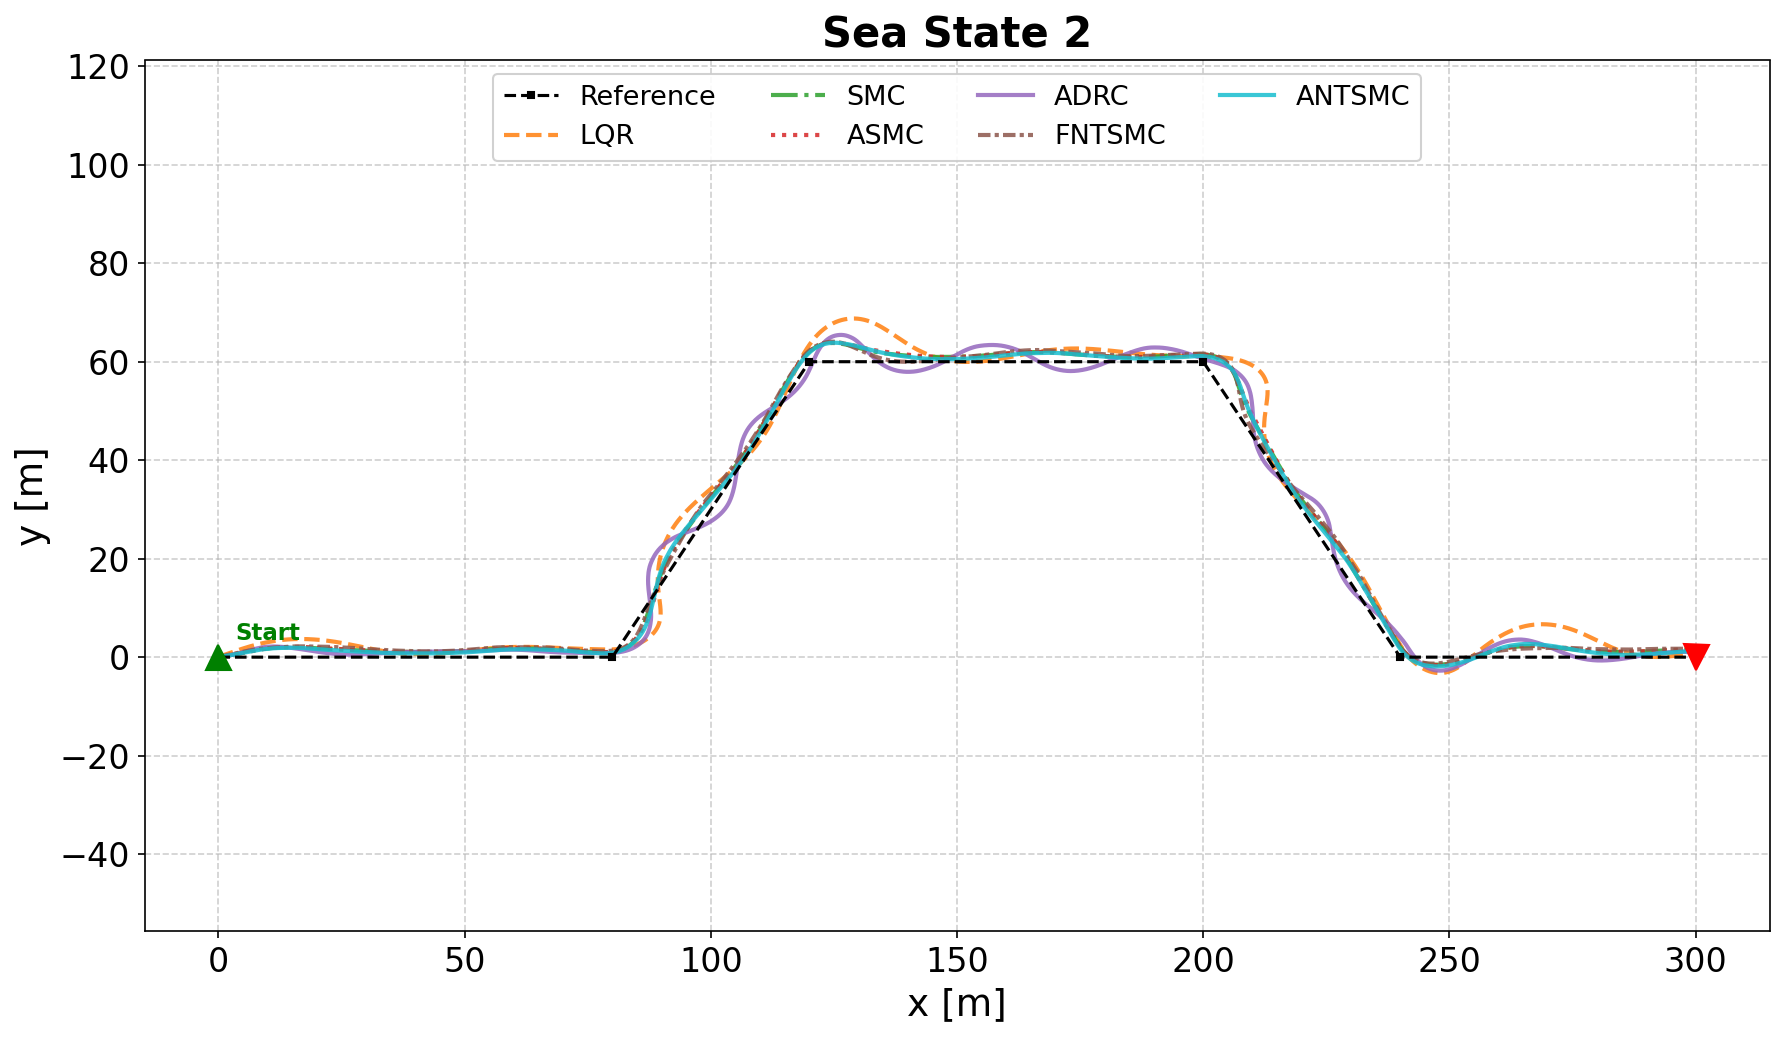
\includegraphics[width=\textwidth]{traj_custom_ss2.png}
  \caption{Custom path.}
\end{subfigure}\hfill
\begin{subfigure}[b]{0.48\textwidth}
  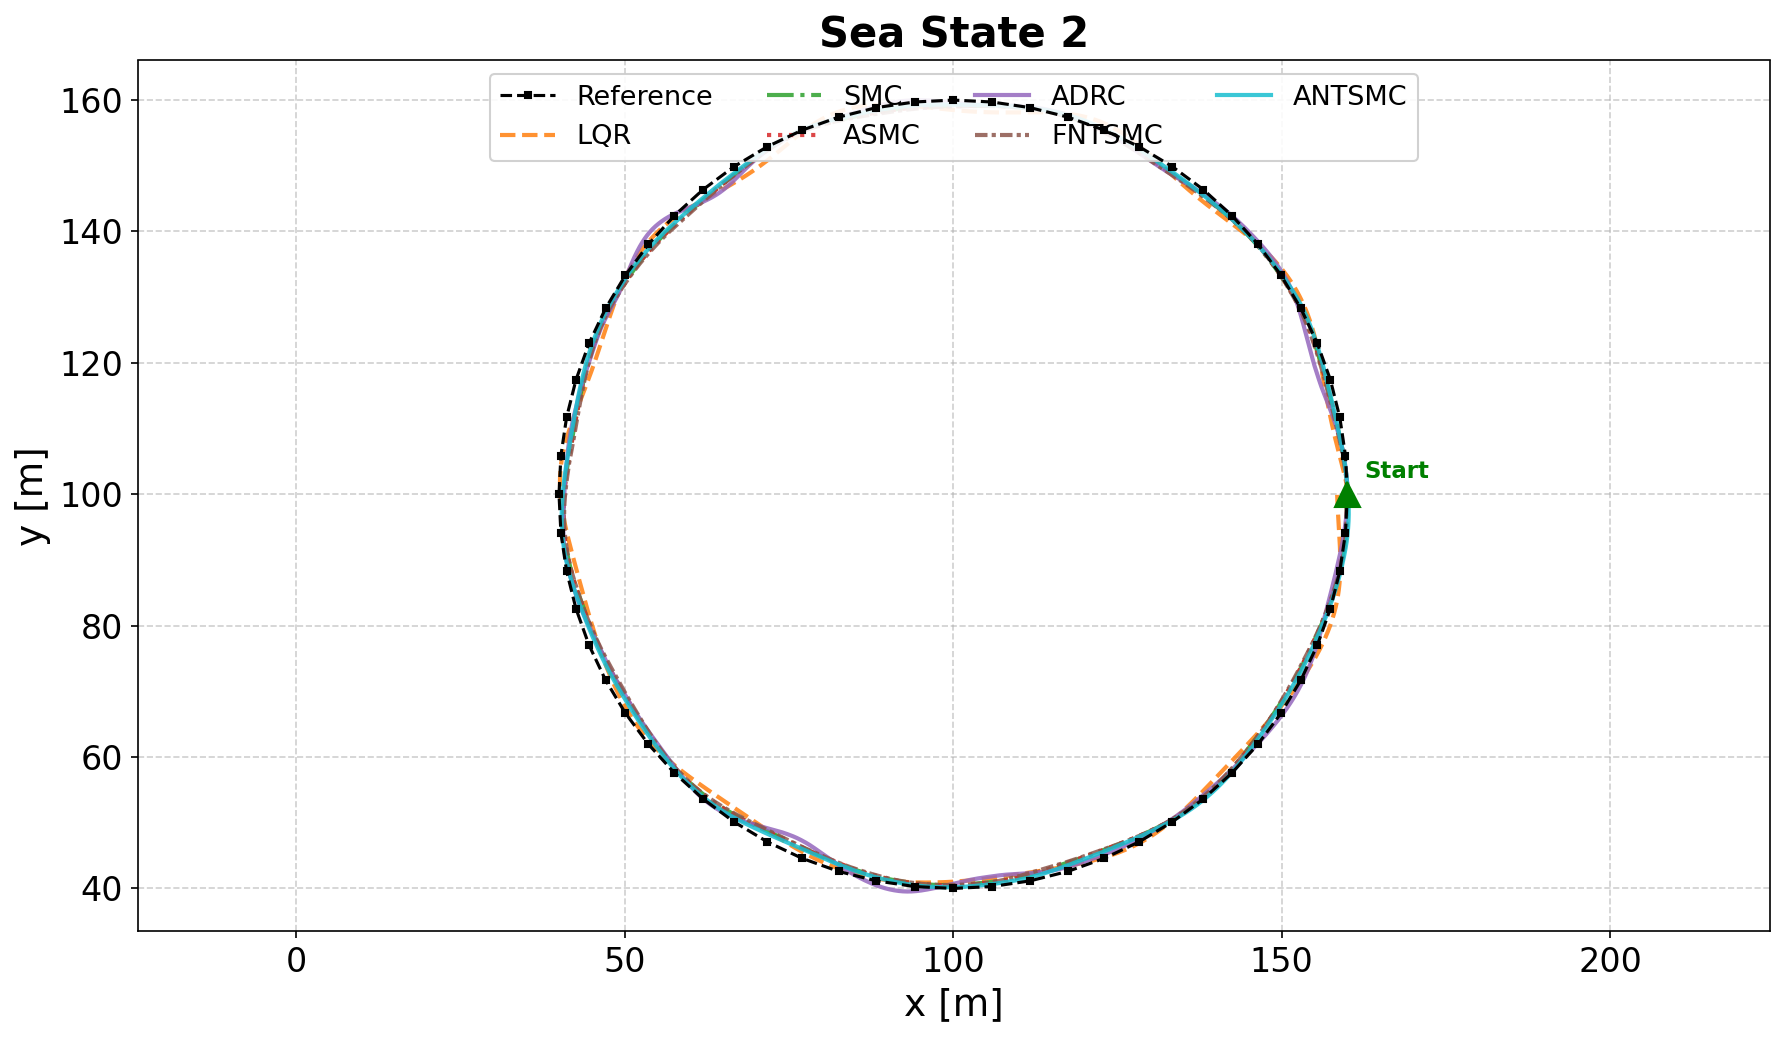
\includegraphics[width=\textwidth]{traj_circular_ss2.png}
  \caption{Circular path.}
\end{subfigure}\\[6pt]
\begin{subfigure}[b]{0.48\textwidth}
  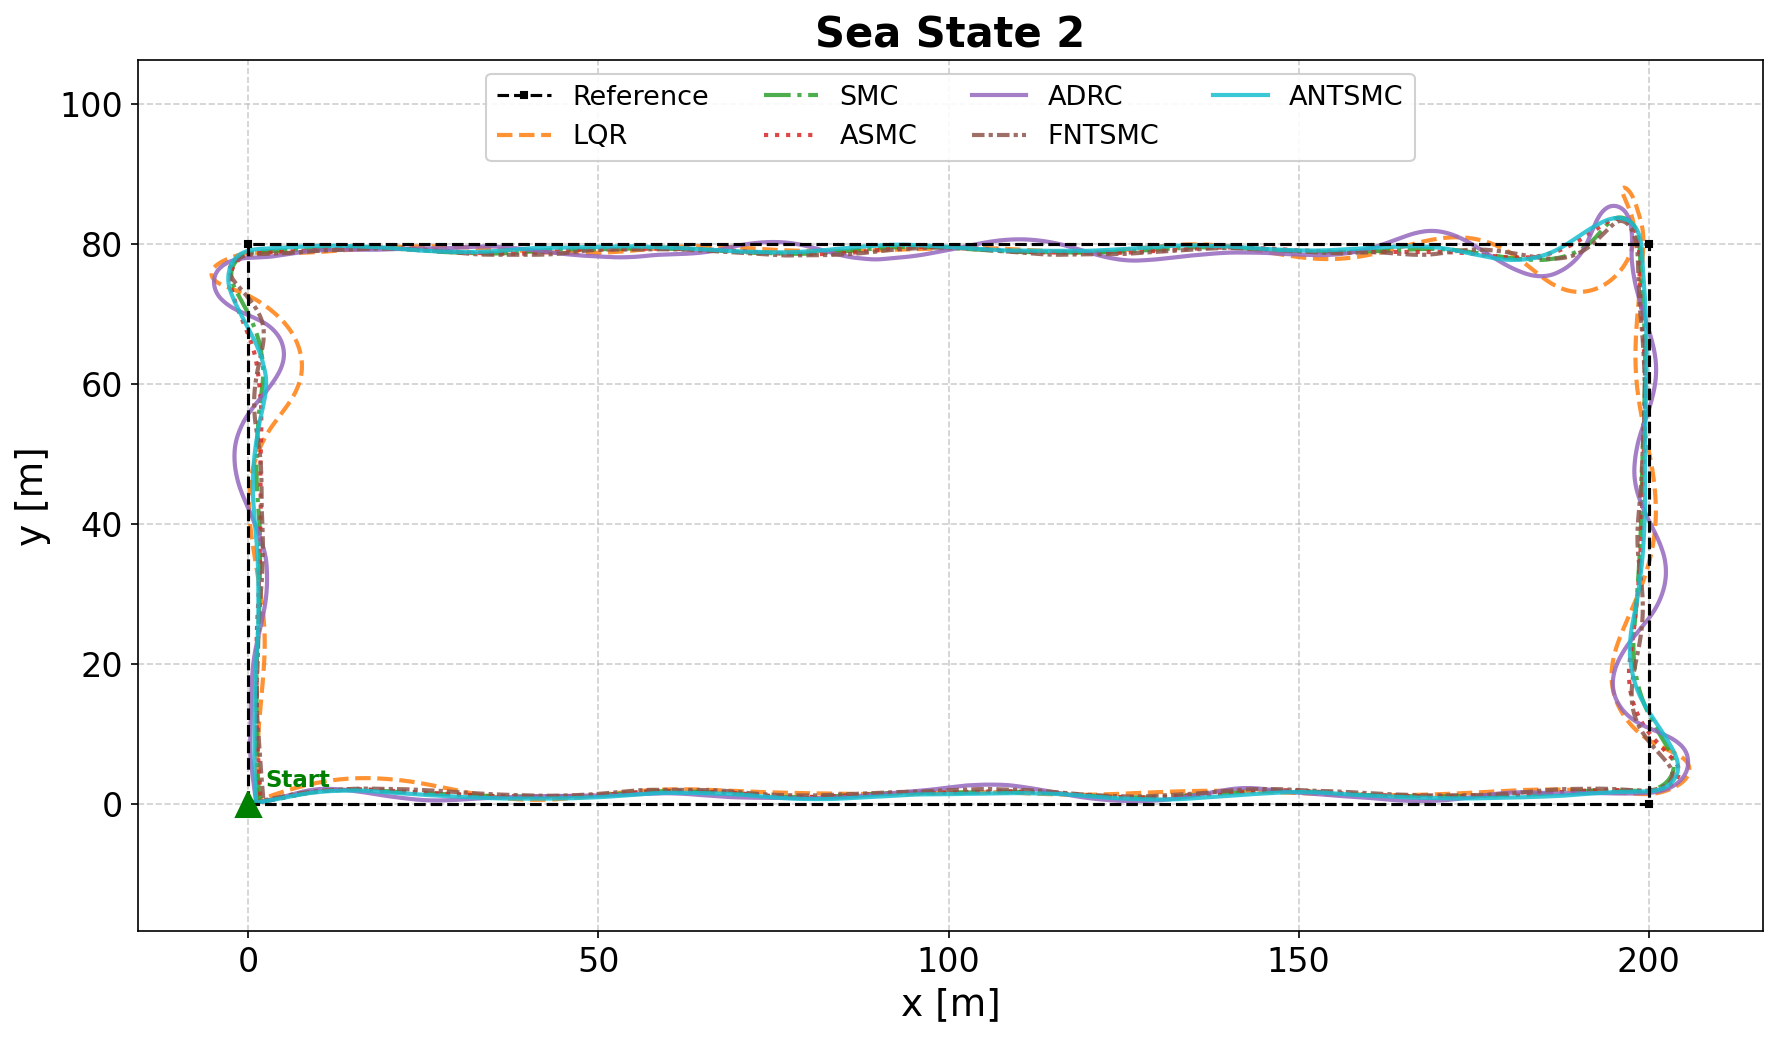
\includegraphics[width=\textwidth]{traj_rectangular_ss2.png}
  \caption{Rectangular path.}
\end{subfigure}\hfill
\begin{subfigure}[b]{0.48\textwidth}
  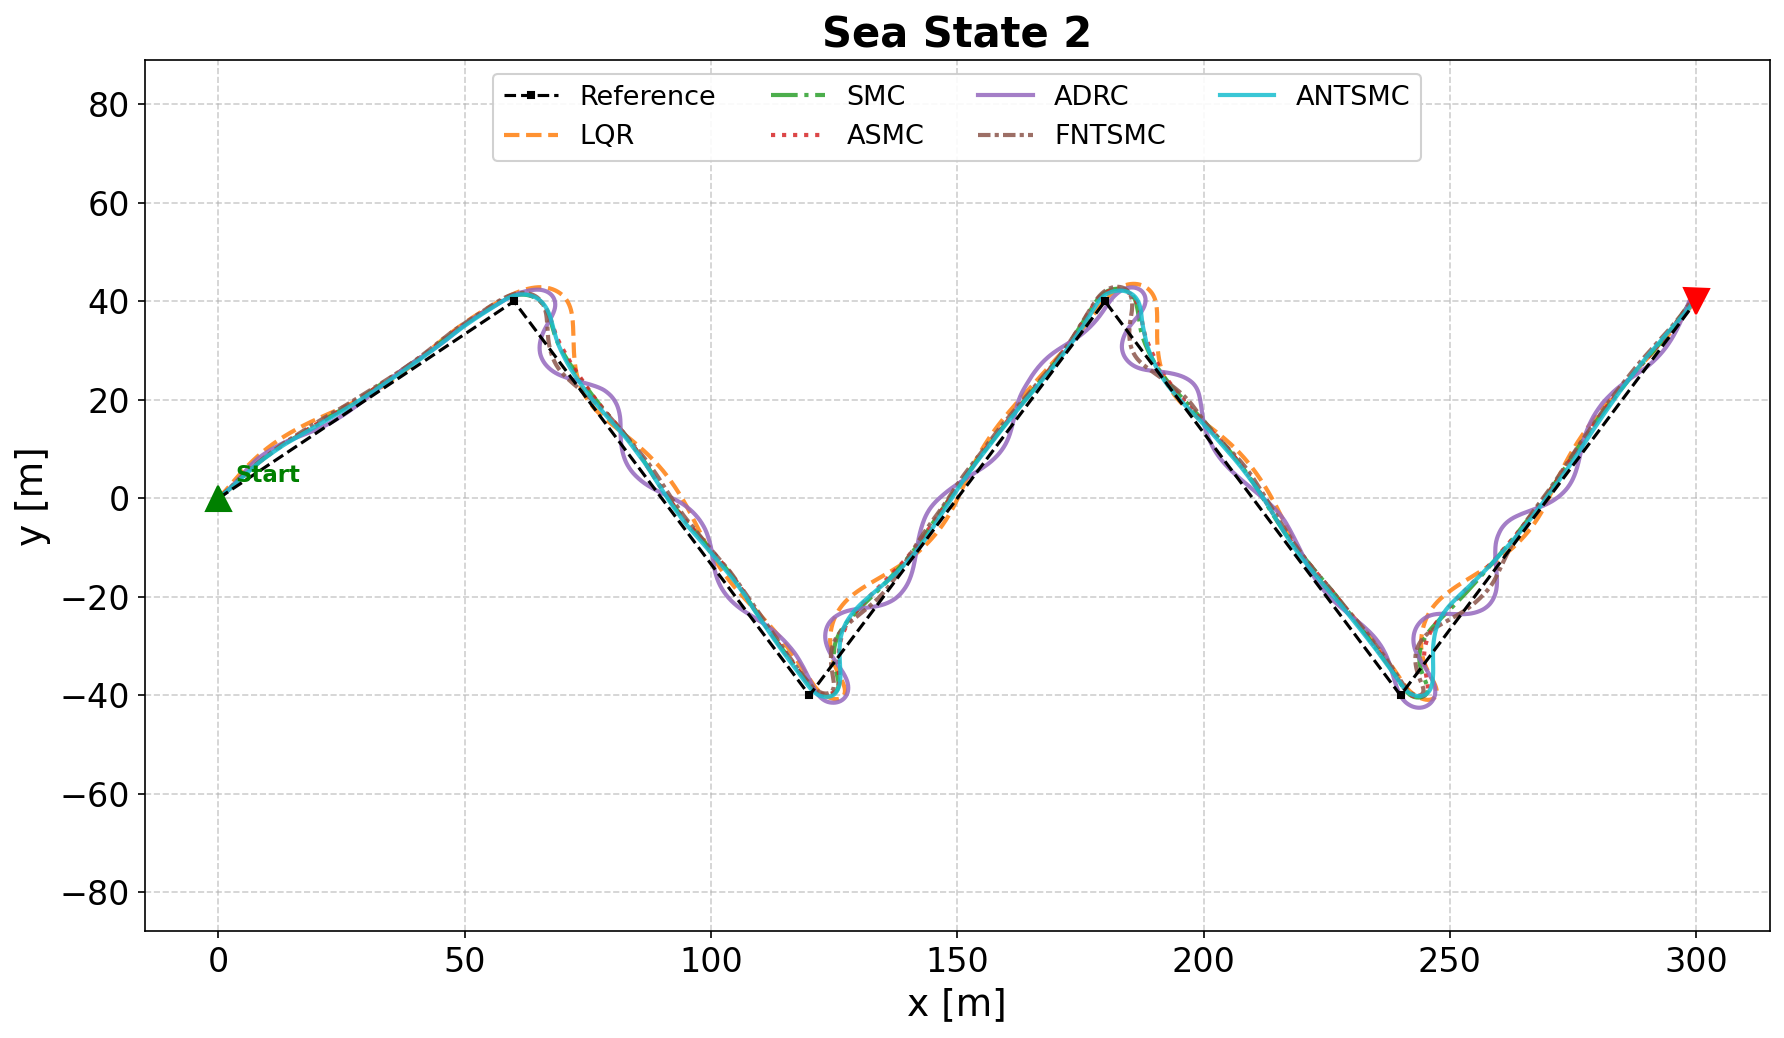
\includegraphics[width=\textwidth]{traj_zigzag_ss2.png}
  \caption{Zigzag path.}
\end{subfigure}
\caption{Trajectory tracking at Sea State~2 for all four path geometries. ANTSMC and SMC maintain tight tracking; LQR shows amplified deviations under moderate disturbances. FNTSMC and ASMC perform comparably to SMC.}
\label{fig:traj_ss2}
\end{figure*}

\subsubsection{Cross-Track Error at SS\,2}

Fig.~\ref{fig:ye_ss2} shows the cross-track error at SS\,2. ANTSMC achieves the tightest error envelope on all paths. The error envelope of ANTSMC remains below $\pm 4$~m while LQR exceeds $\pm 8$~m on the custom path.

\begin{figure*}[t]
\centering
\begin{subfigure}[b]{0.48\textwidth}
  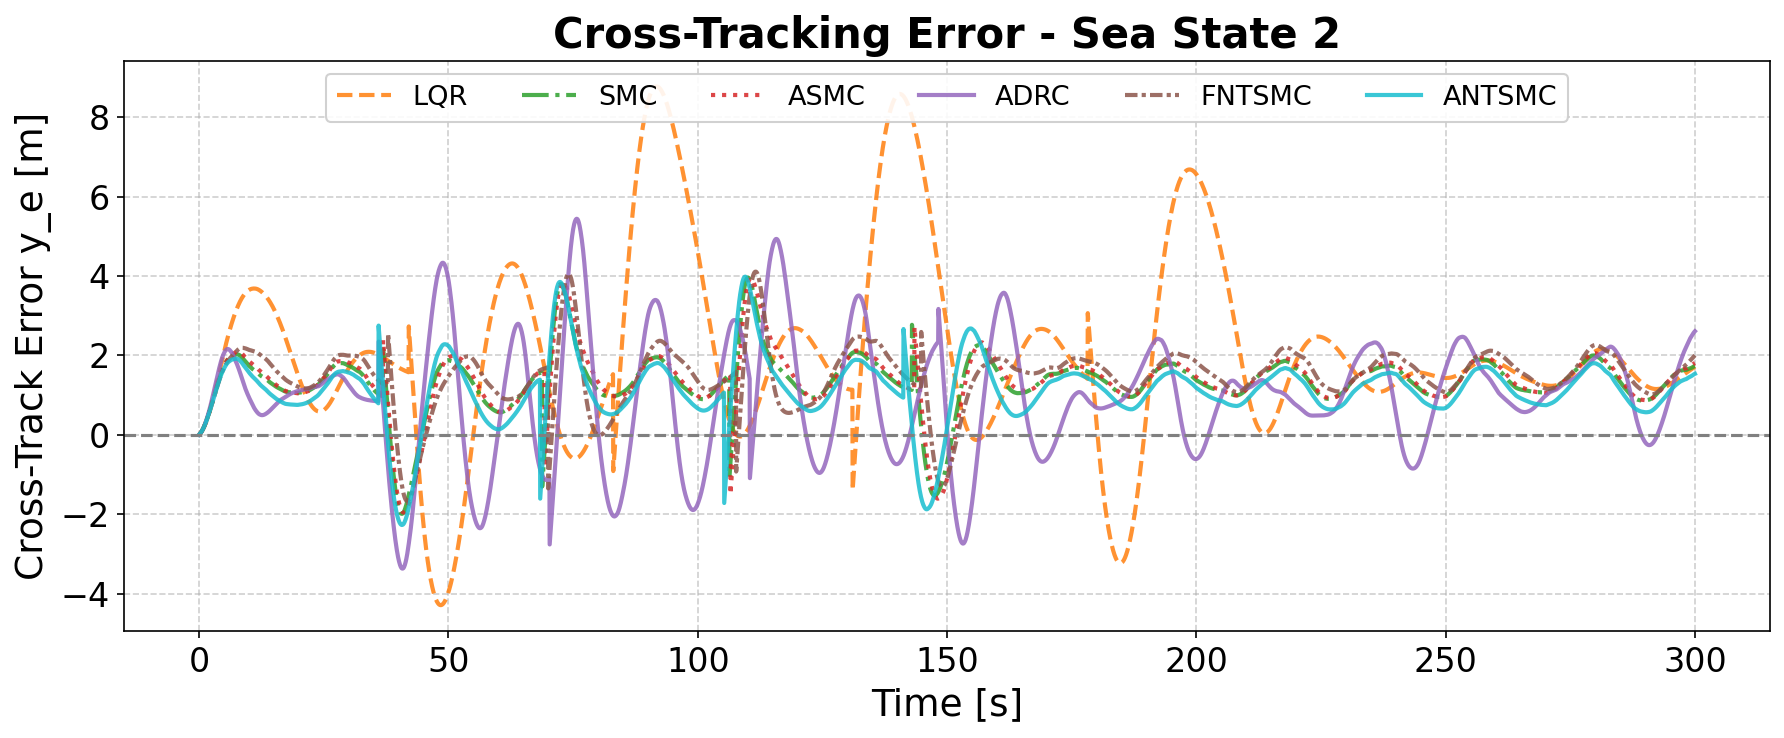
\includegraphics[width=\textwidth]{error_custom_ss2.png}
  \caption{Custom path.}
\end{subfigure}\hfill
\begin{subfigure}[b]{0.48\textwidth}
  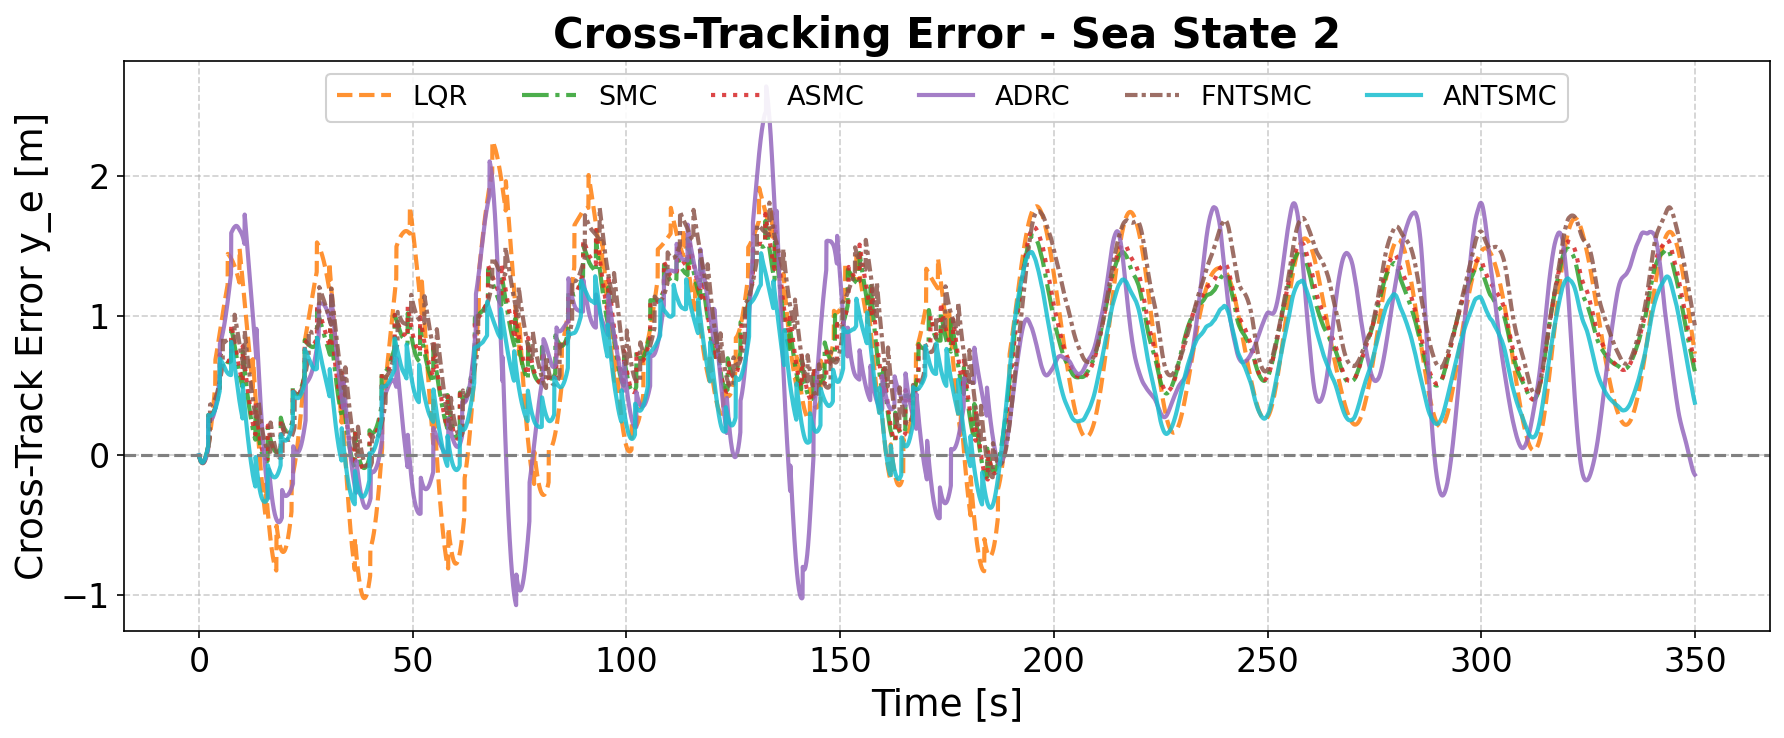
\includegraphics[width=\textwidth]{error_circular_ss2.png}
  \caption{Circular path.}
\end{subfigure}\\[6pt]
\begin{subfigure}[b]{0.48\textwidth}
  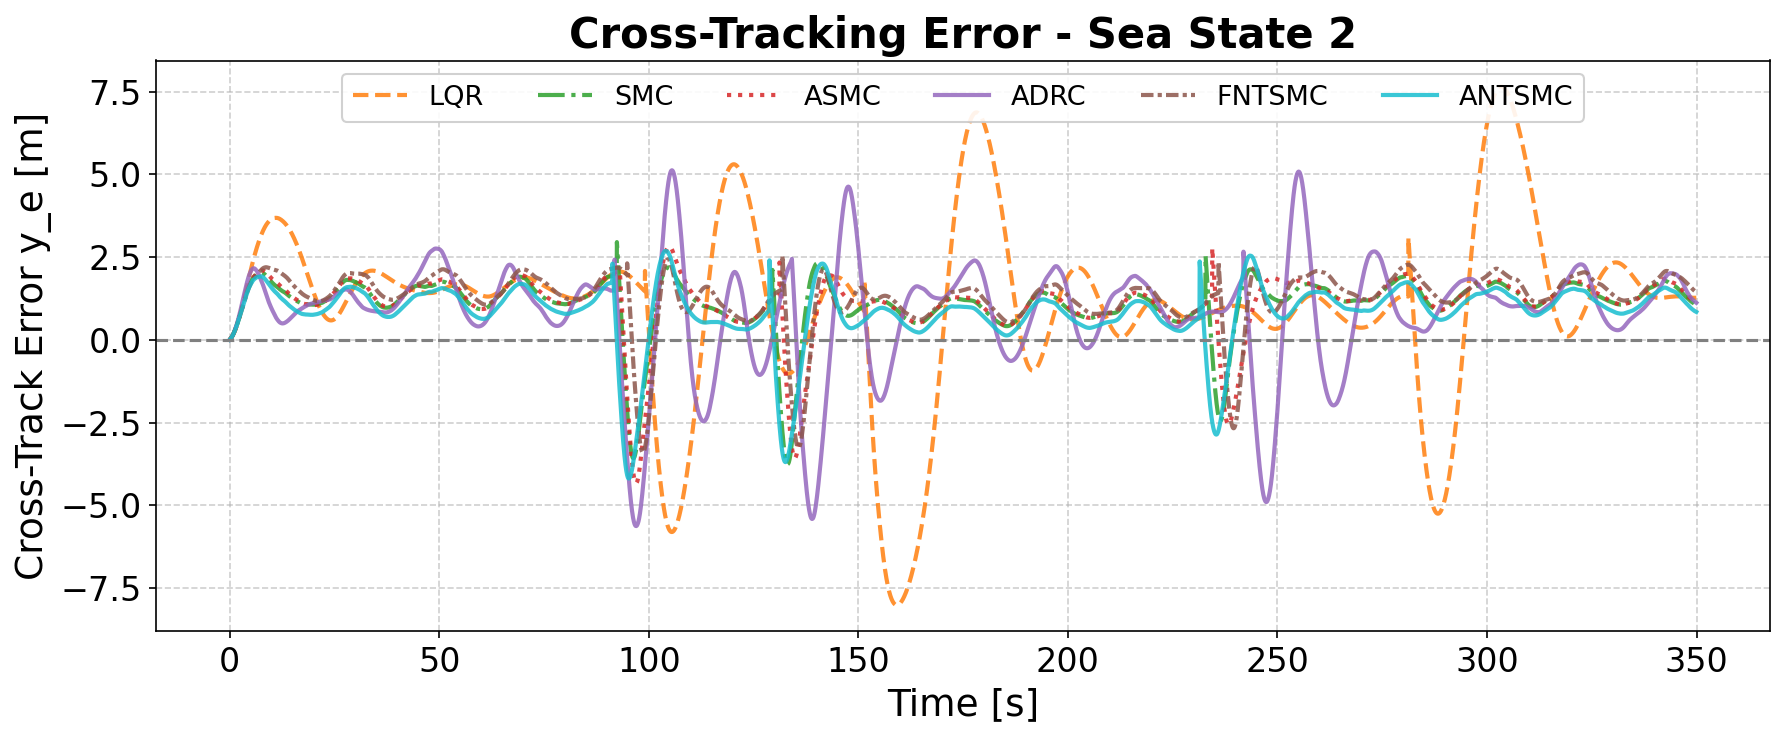
\includegraphics[width=\textwidth]{error_rectangular_ss2.png}
  \caption{Rectangular path.}
\end{subfigure}\hfill
\begin{subfigure}[b]{0.48\textwidth}
  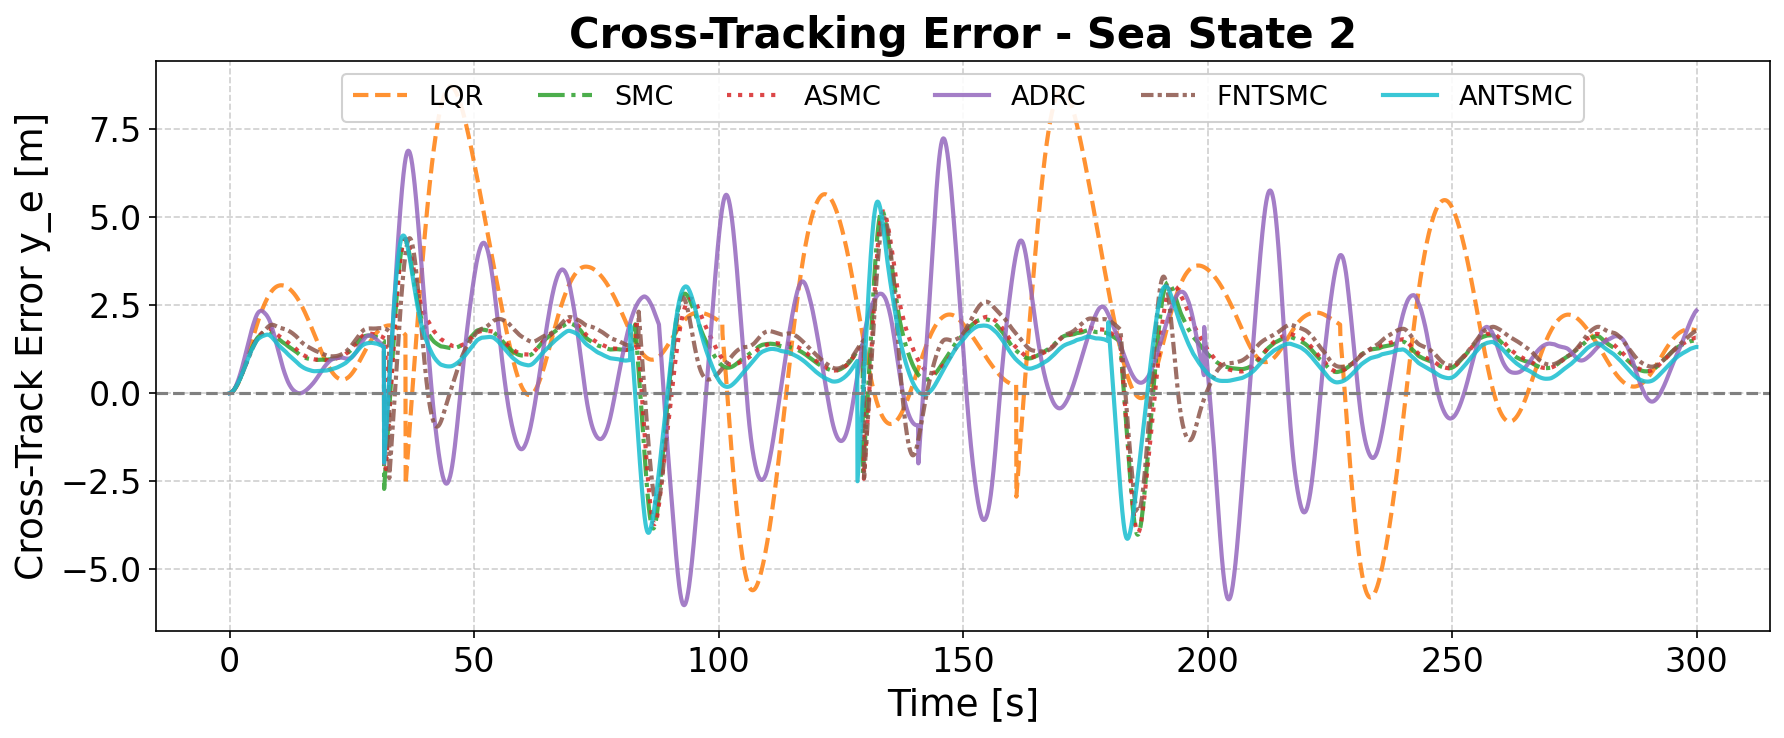
\includegraphics[width=\textwidth]{error_zigzag_ss2.png}
  \caption{Zigzag path.}
\end{subfigure}
\caption{Cross-track error $y_e(t)$ at Sea State~2 for all four paths. ANTSMC achieves the tightest error envelope, with the gap over baselines widening compared to SS\,1.}
\label{fig:ye_ss2}
\end{figure*}

\subsubsection{Heading Tracking at SS\,2}

Fig.~\ref{fig:heading_ss2} presents the heading responses at SS\,2. ADRC's ESO lag becomes more pronounced under increased disturbances, while ANTSMC's adaptive gain provides smooth heading tracking. FNTSMC's FTDO-based compensation provides good heading tracking on smooth segments but introduces slight transient artefacts at corners.

\begin{figure*}[t]
\centering
\begin{subfigure}[b]{0.48\textwidth}
  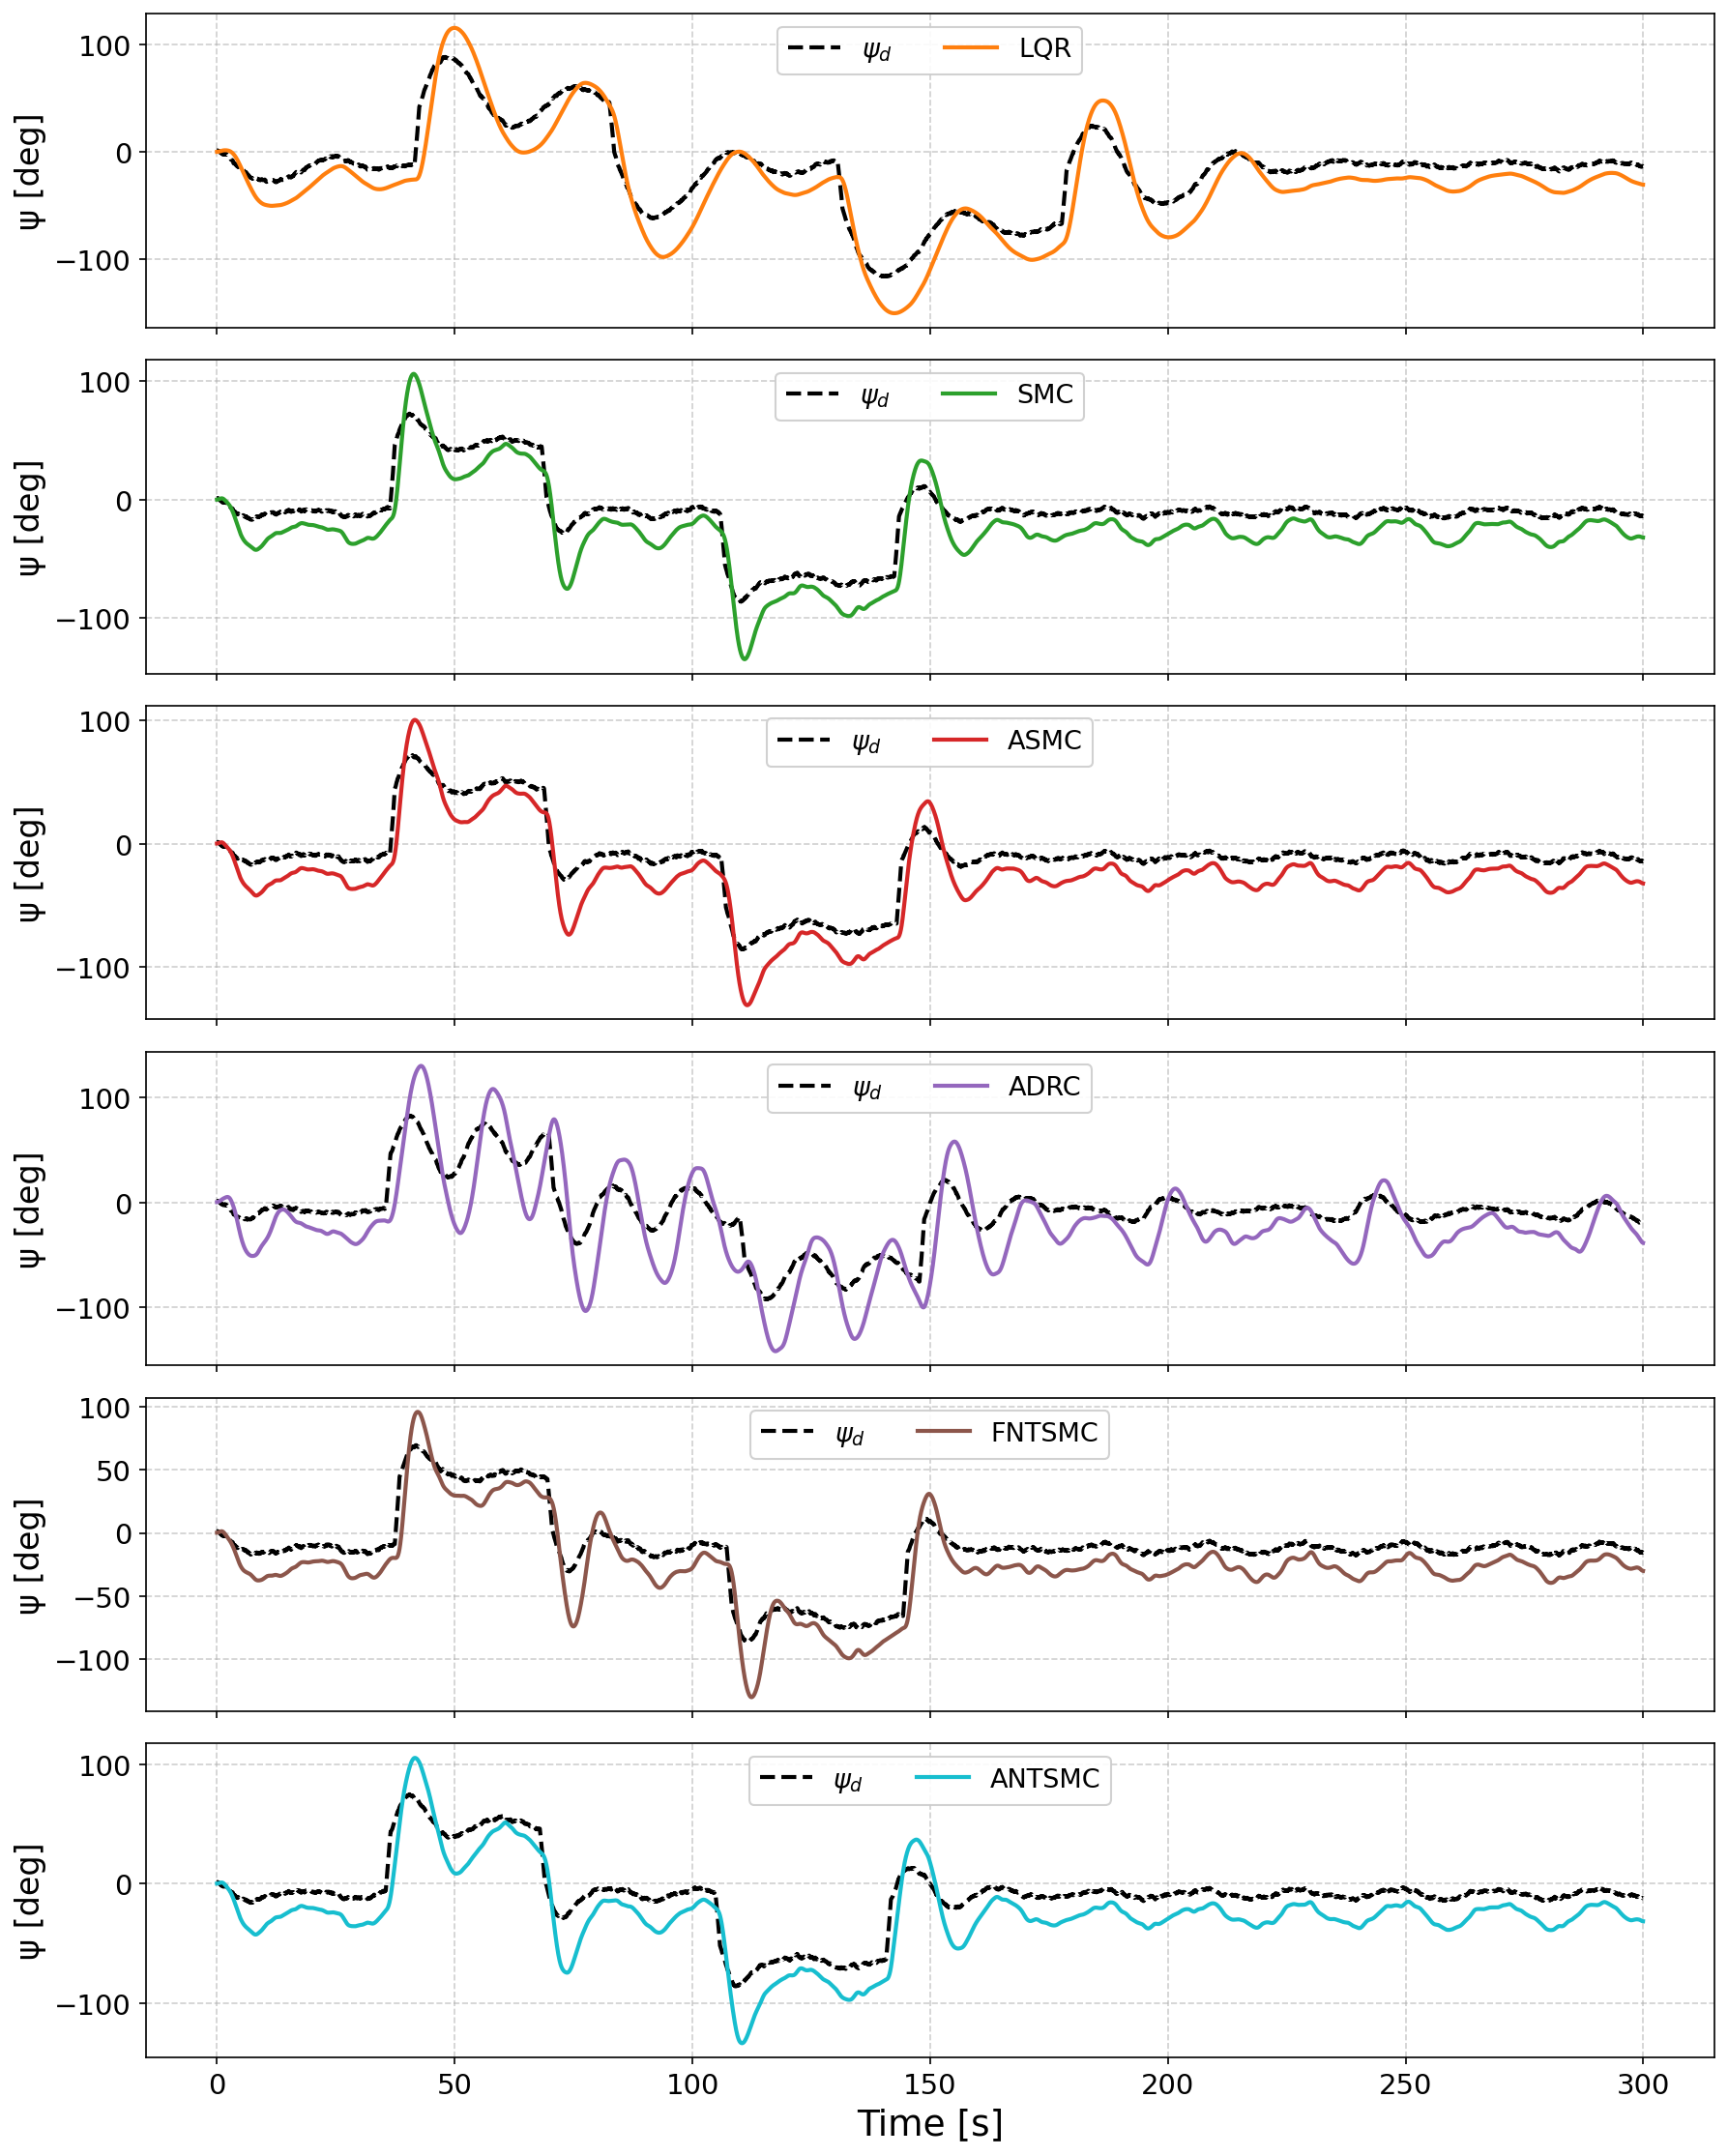
\includegraphics[width=\textwidth]{heading_custom_ss2.png}
  \caption{Custom path.}
\end{subfigure}\hfill
\begin{subfigure}[b]{0.48\textwidth}
  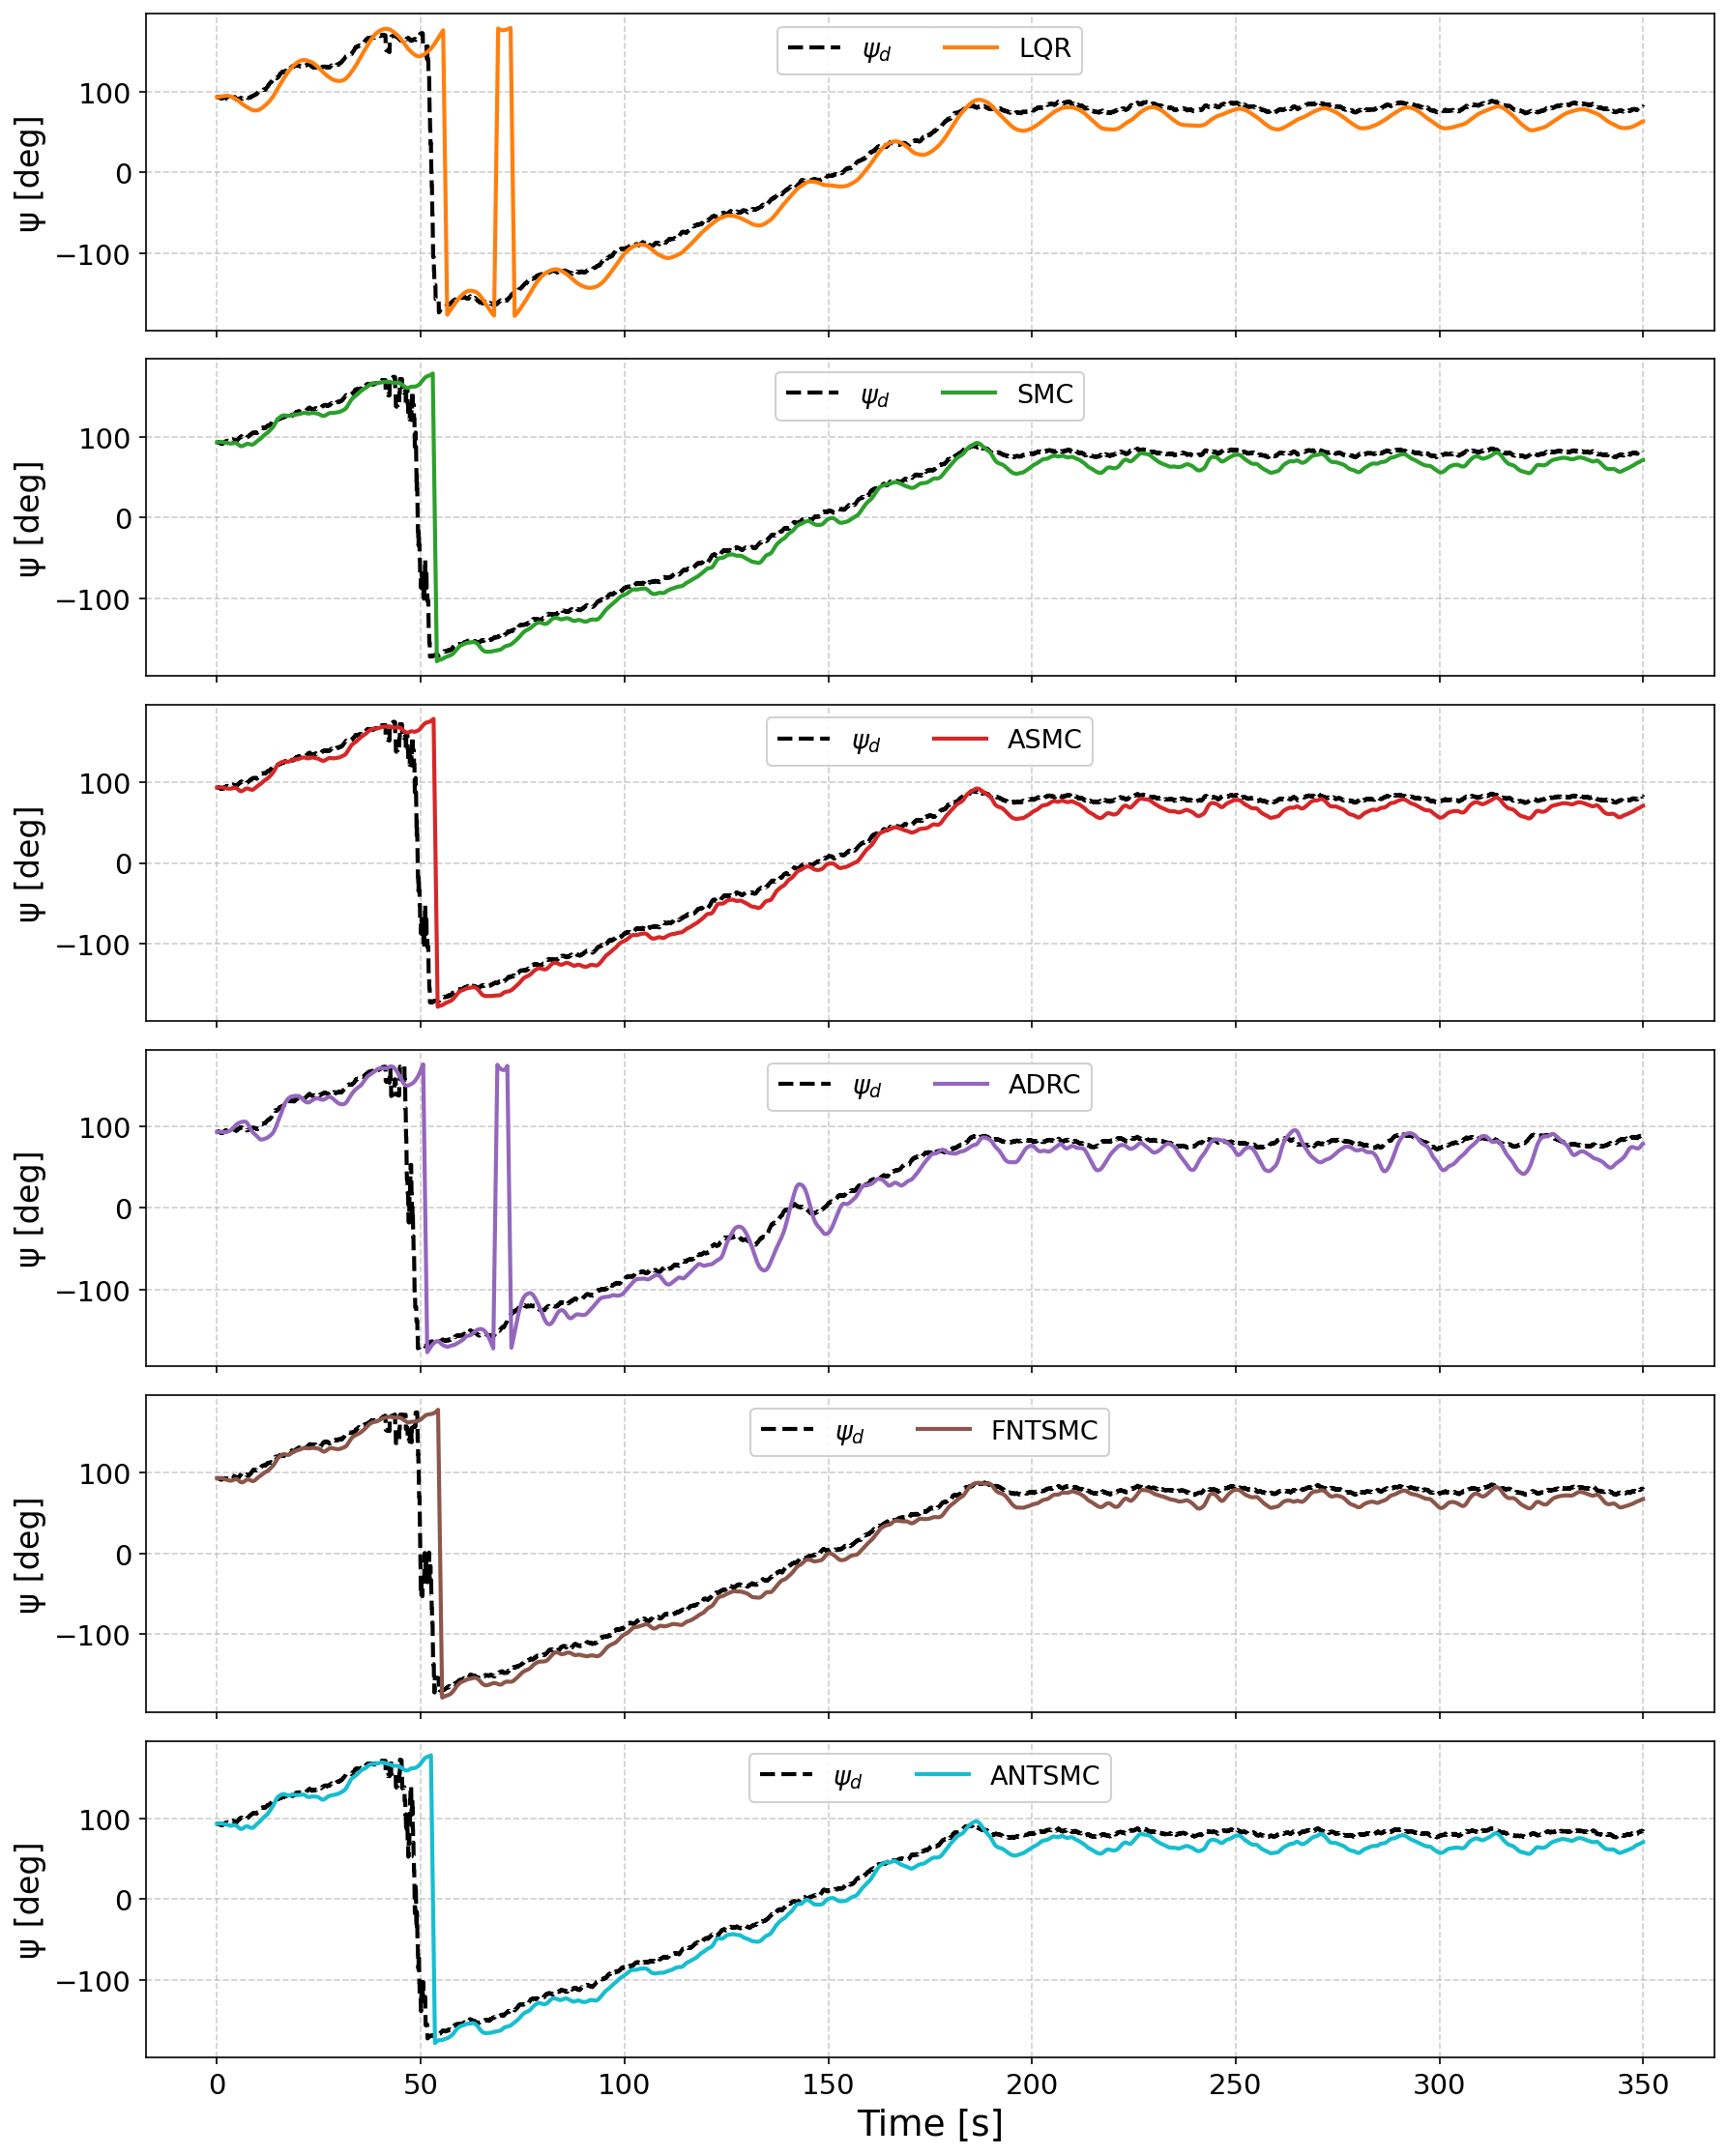
\includegraphics[width=\textwidth]{heading_circular_ss2.png}
  \caption{Circular path.}
\end{subfigure}\\[6pt]
\begin{subfigure}[b]{0.48\textwidth}
  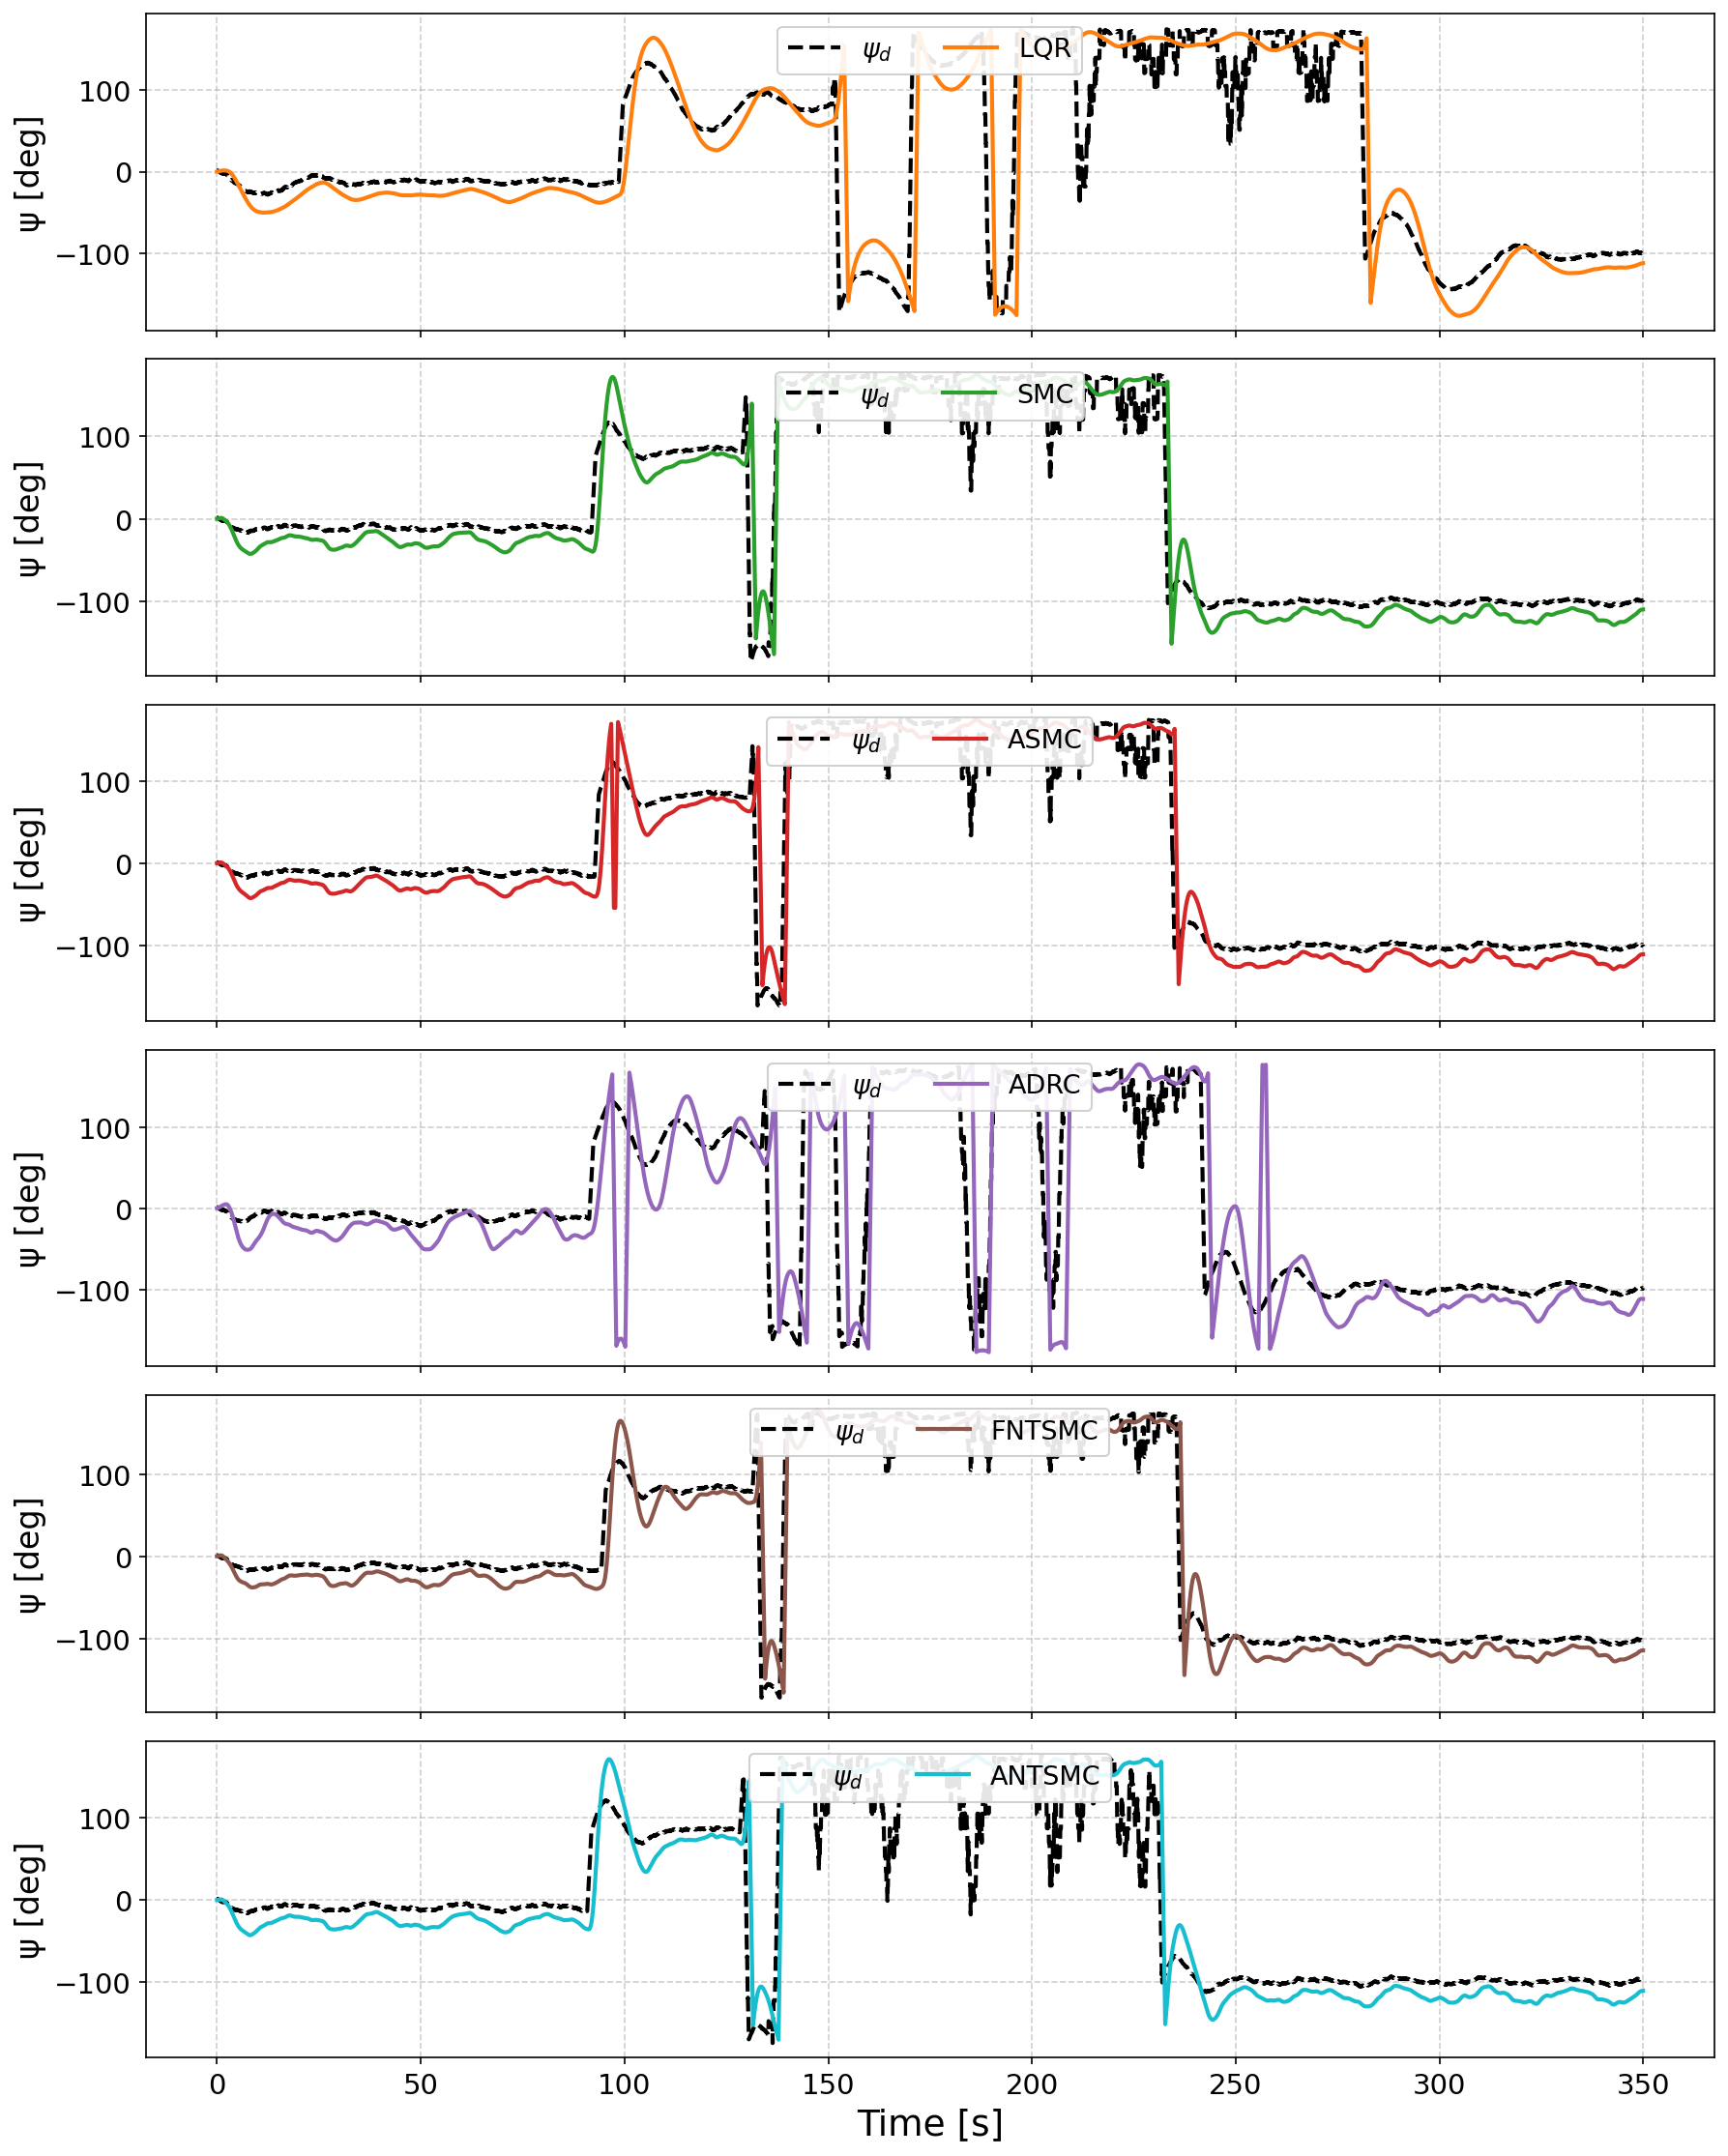
\includegraphics[width=\textwidth]{heading_rectangular_ss2.png}
  \caption{Rectangular path.}
\end{subfigure}\hfill
\begin{subfigure}[b]{0.48\textwidth}
  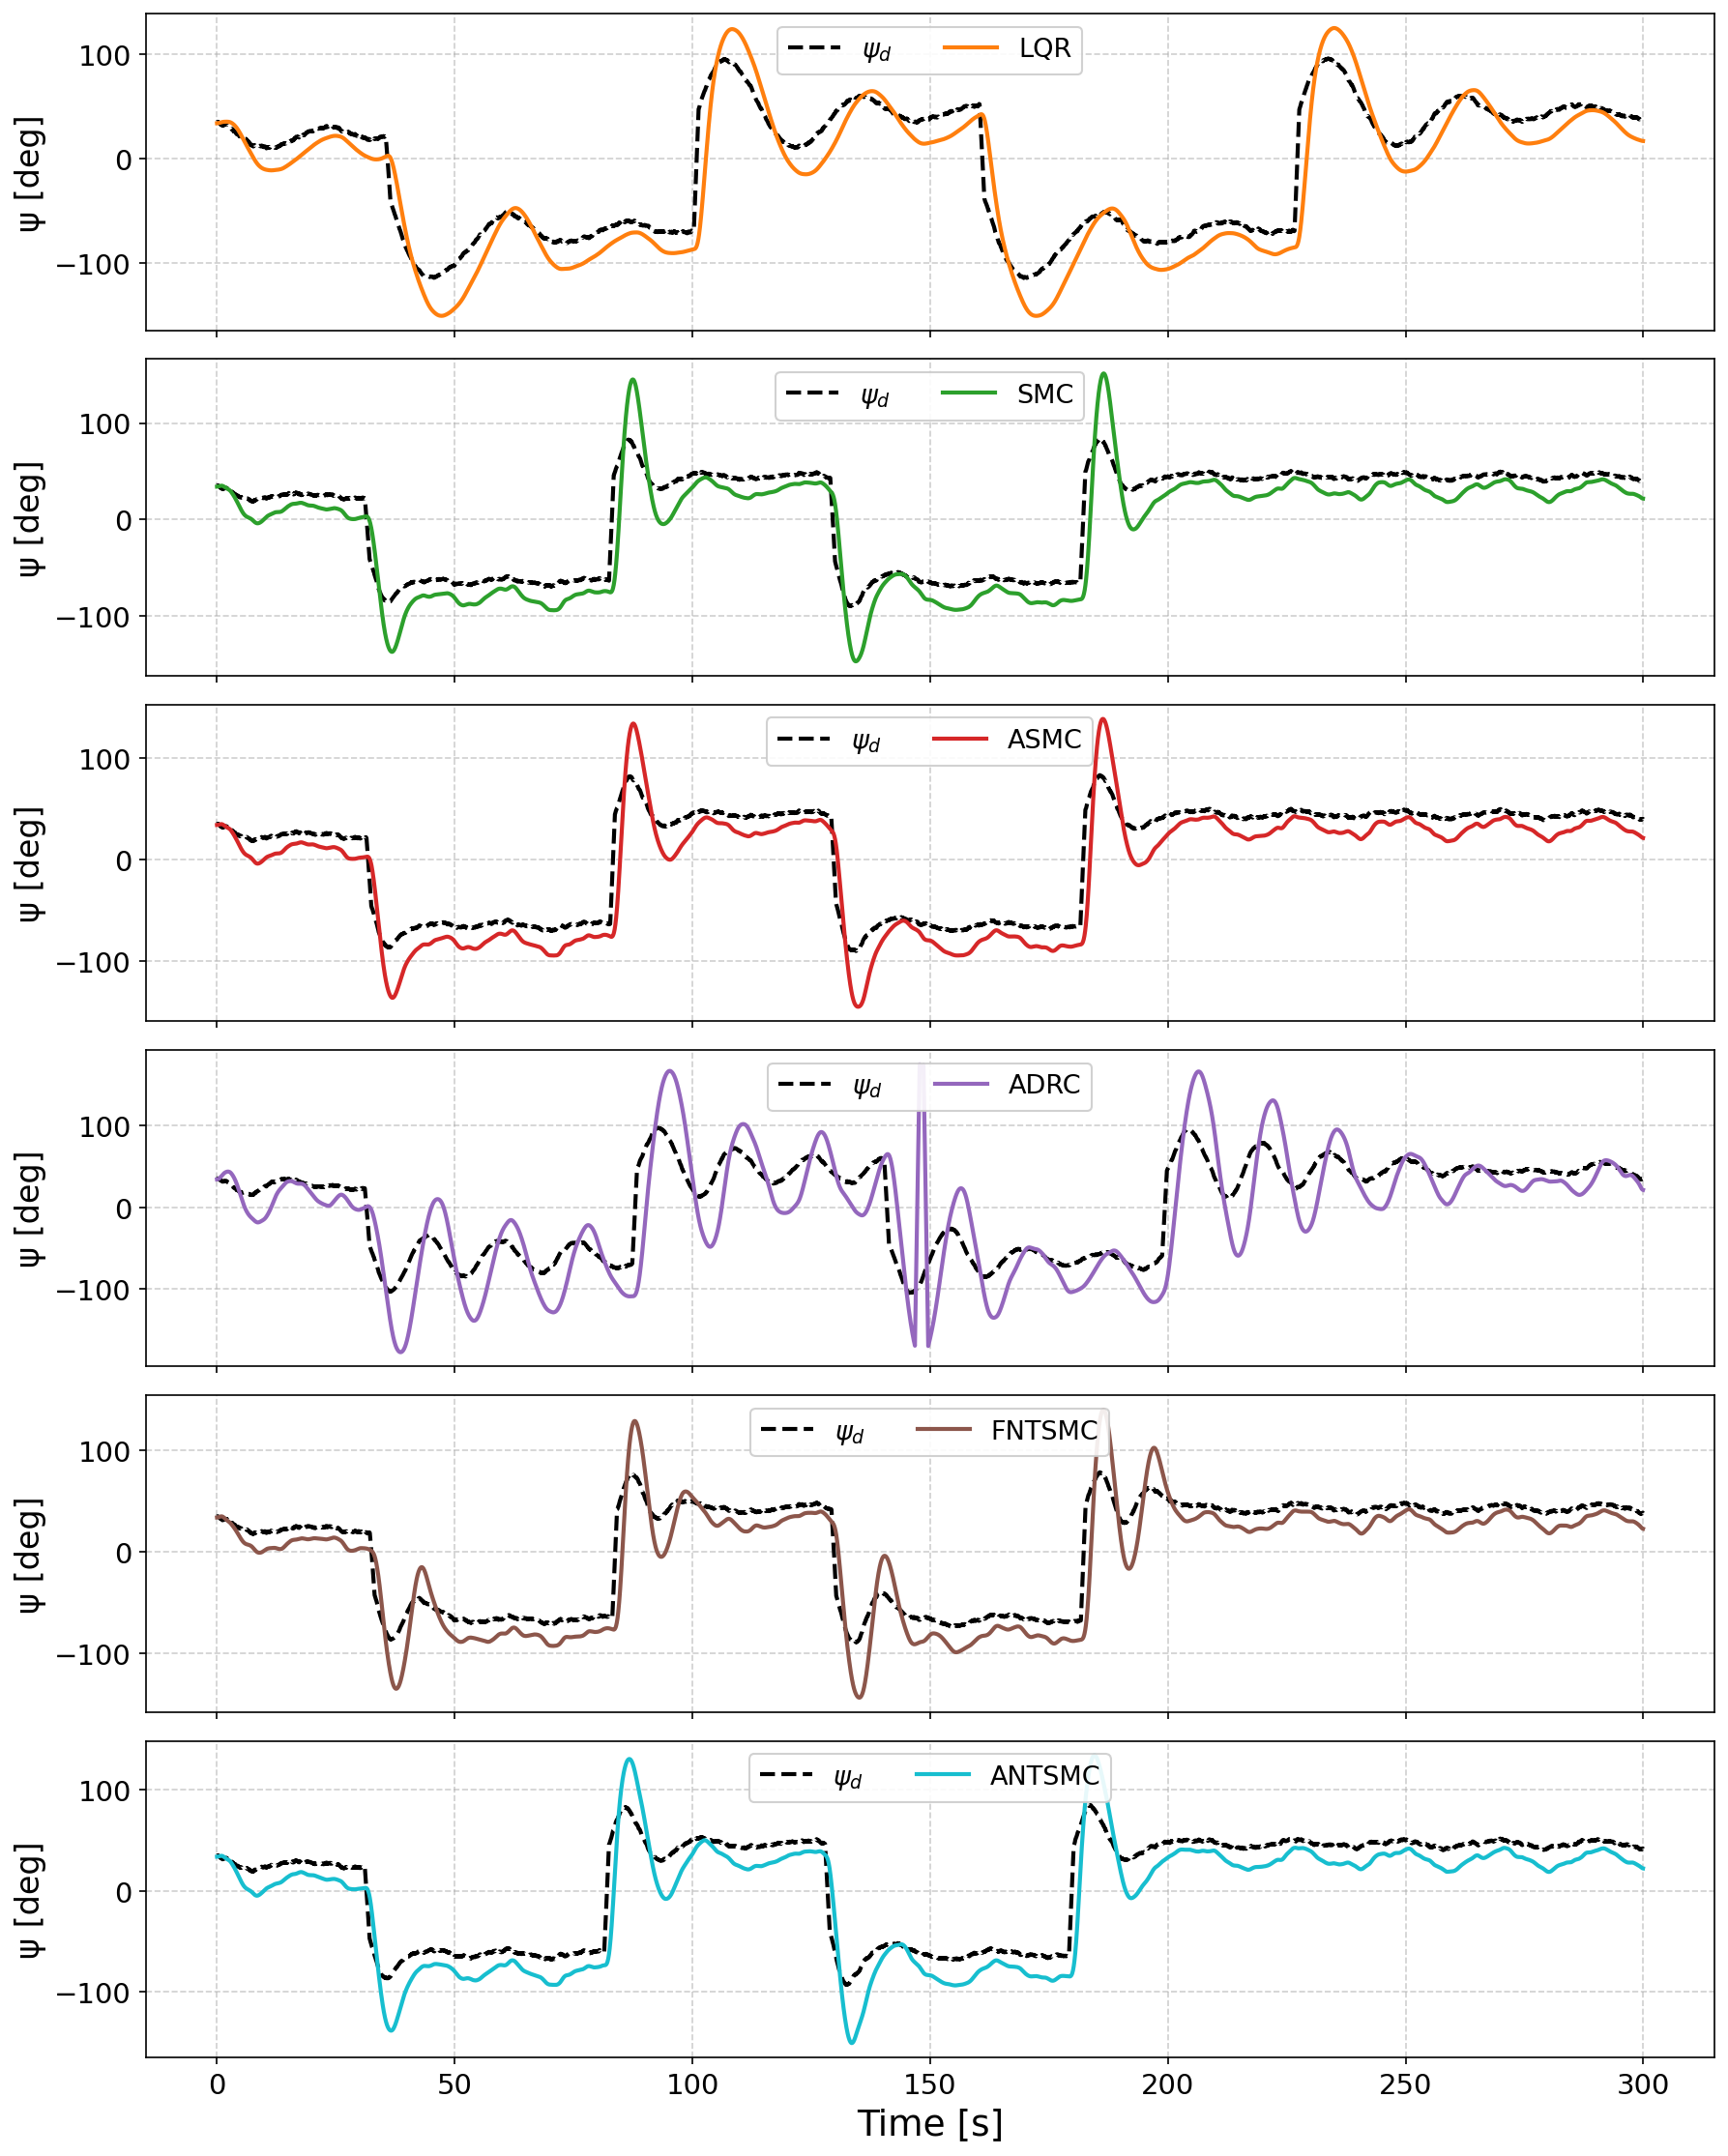
\includegraphics[width=\textwidth]{heading_zigzag_ss2.png}
  \caption{Zigzag path.}
\end{subfigure}
\caption{Heading tracking at Sea State~2 for all four paths. Each subplot shows an individual controller's heading response against its desired heading. ADRC's ESO lag becomes more pronounced; ANTSMC provides smooth heading tracking.}
\label{fig:heading_ss2}
\end{figure*}

\subsubsection{Course Tracking at SS\,2}

Fig.~\ref{fig:course_ss2} overlays all controllers' heading responses against the target course angle at SS\,2. ANTSMC tracks the course most closely on all paths, with the gap over baselines widening compared to SS\,1.

\begin{figure*}[t]
\centering
\begin{subfigure}[b]{0.48\textwidth}
  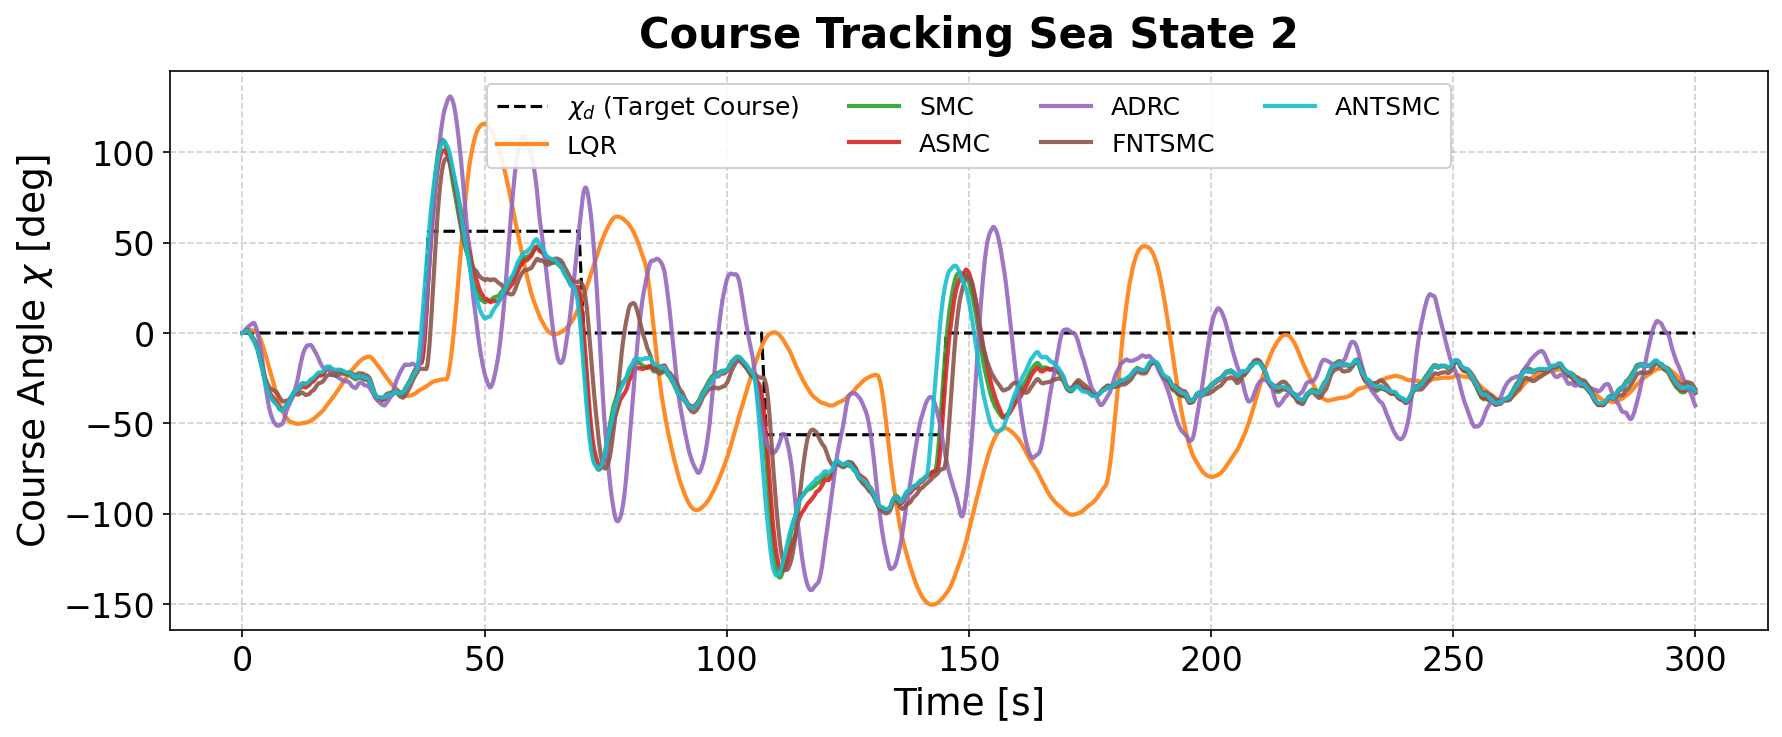
\includegraphics[width=\textwidth]{course_custom_ss2.png}
  \caption{Custom path.}
\end{subfigure}\hfill
\begin{subfigure}[b]{0.48\textwidth}
  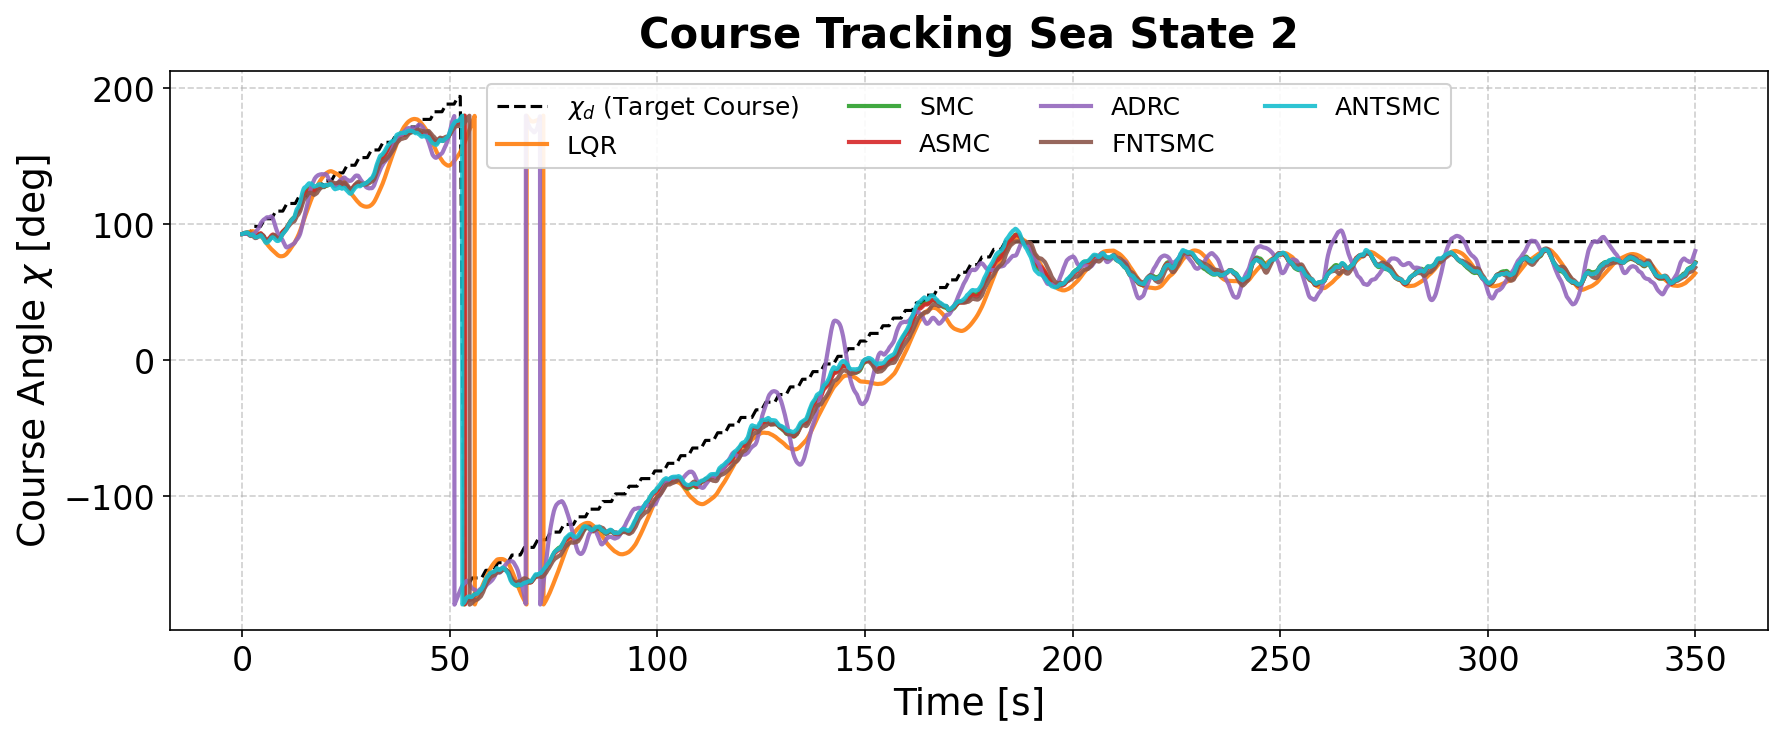
\includegraphics[width=\textwidth]{course_circular_ss2.png}
  \caption{Circular path.}
\end{subfigure}\\[6pt]
\begin{subfigure}[b]{0.48\textwidth}
  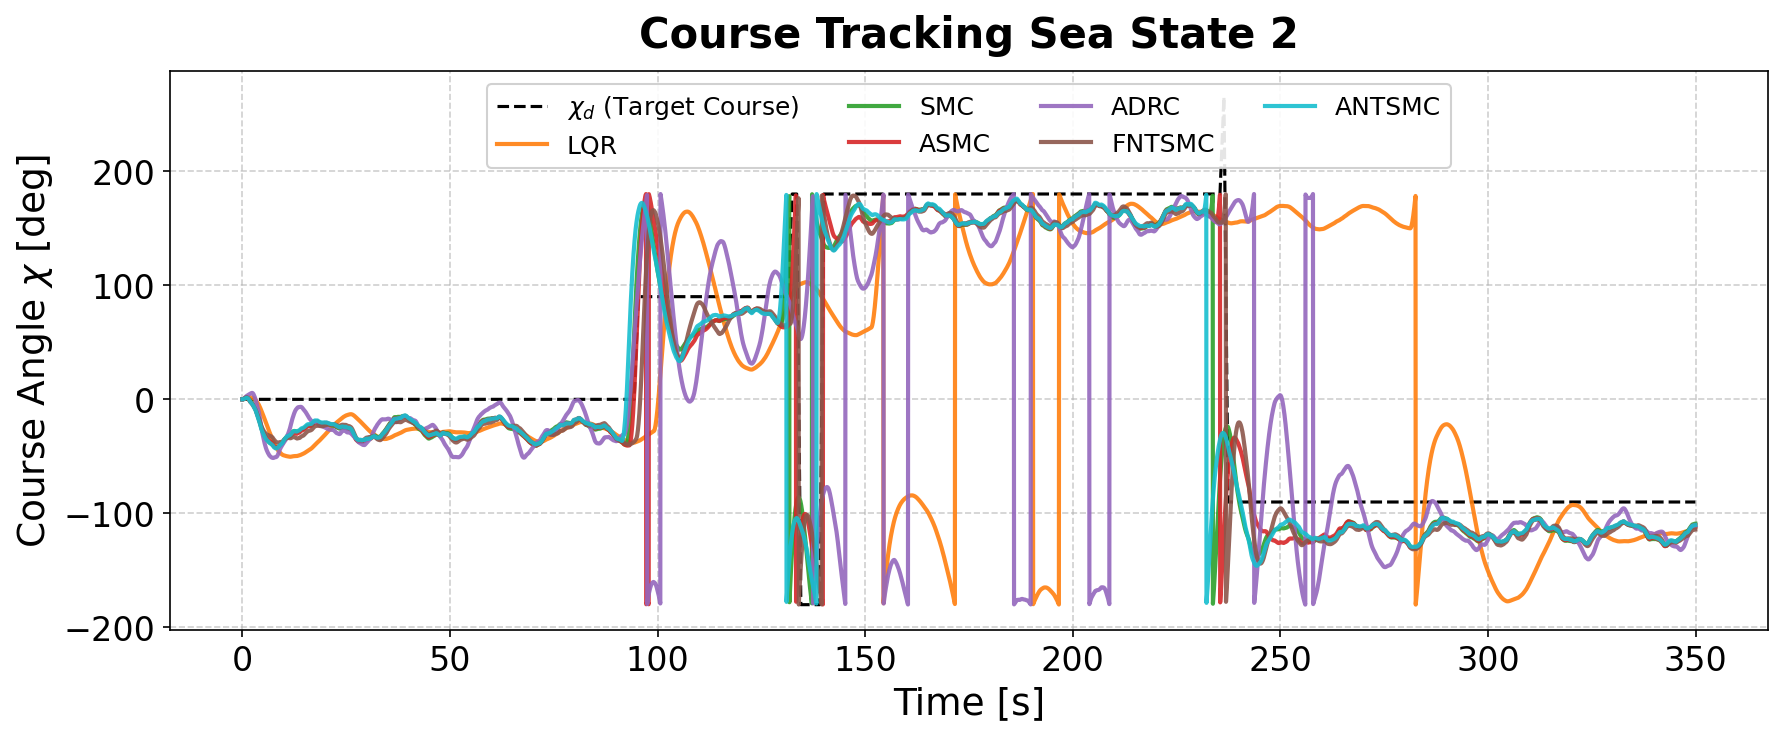
\includegraphics[width=\textwidth]{course_rectangular_ss2.png}
  \caption{Rectangular path.}
\end{subfigure}\hfill
\begin{subfigure}[b]{0.48\textwidth}
  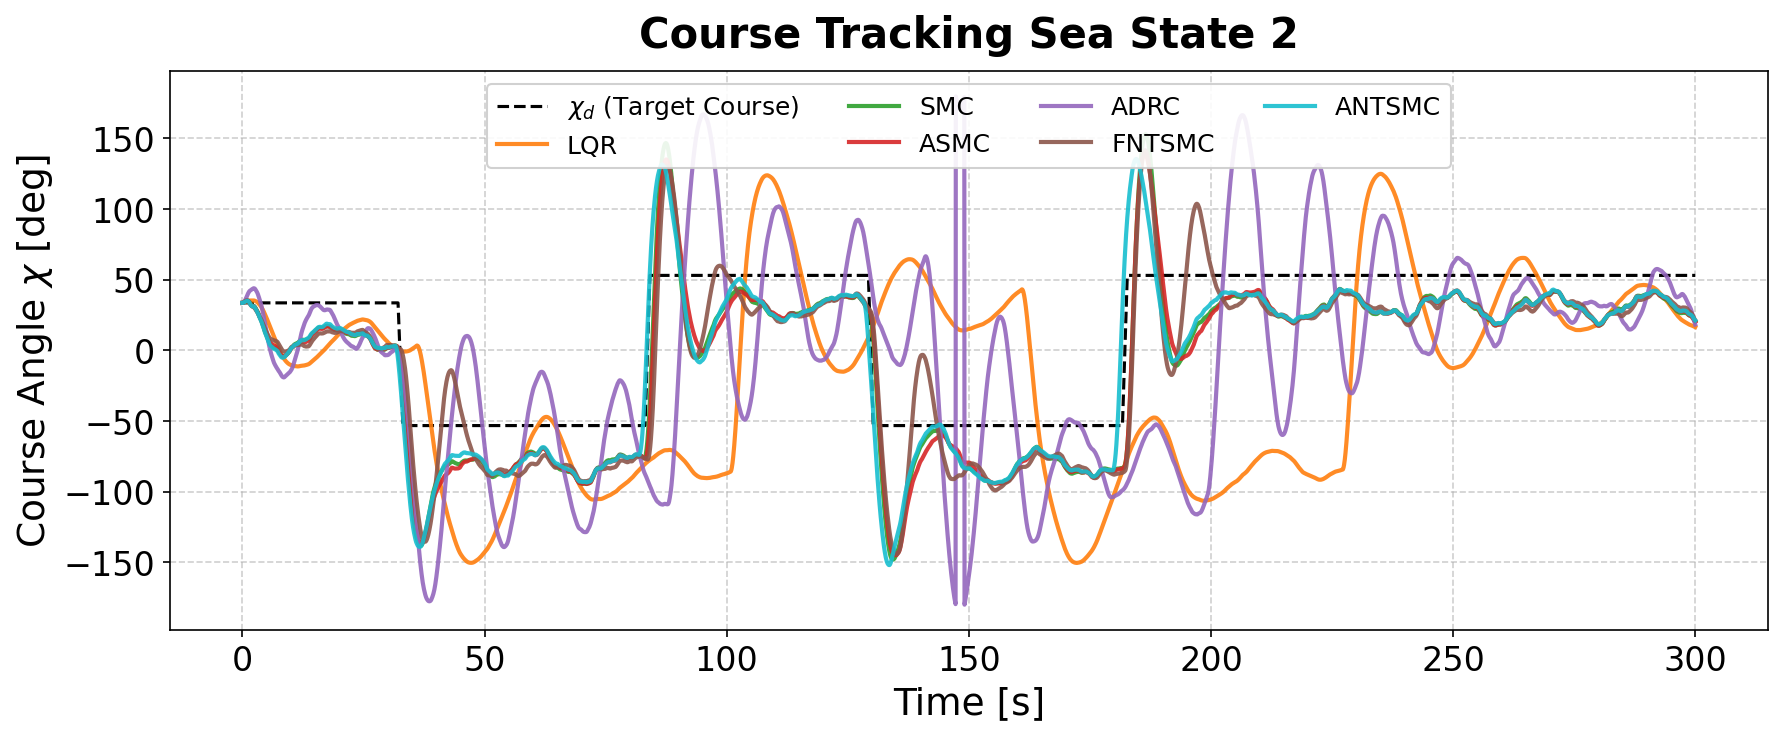
\includegraphics[width=\textwidth]{course_zigzag_ss2.png}
  \caption{Zigzag path.}
\end{subfigure}
\caption{Course tracking at Sea State~2 for all four paths. All controllers' heading responses are overlaid against the target course angle $\gamma$ (black dashed). ANTSMC tracks most faithfully under moderate disturbances, followed closely by SMC and ASMC.}
\label{fig:course_ss2}
\end{figure*}

\subsubsection{Control Effort at SS\,2}

Fig.~\ref{fig:ctrl_ss2} shows the control effort at SS\,2. ANTSMC's adaptive gain increases to $k_{s,r} \approx 0.7$--$0.9$, providing additional robustness without excessive chattering.

\begin{figure*}[t]
\centering
\begin{subfigure}[b]{0.48\textwidth}
  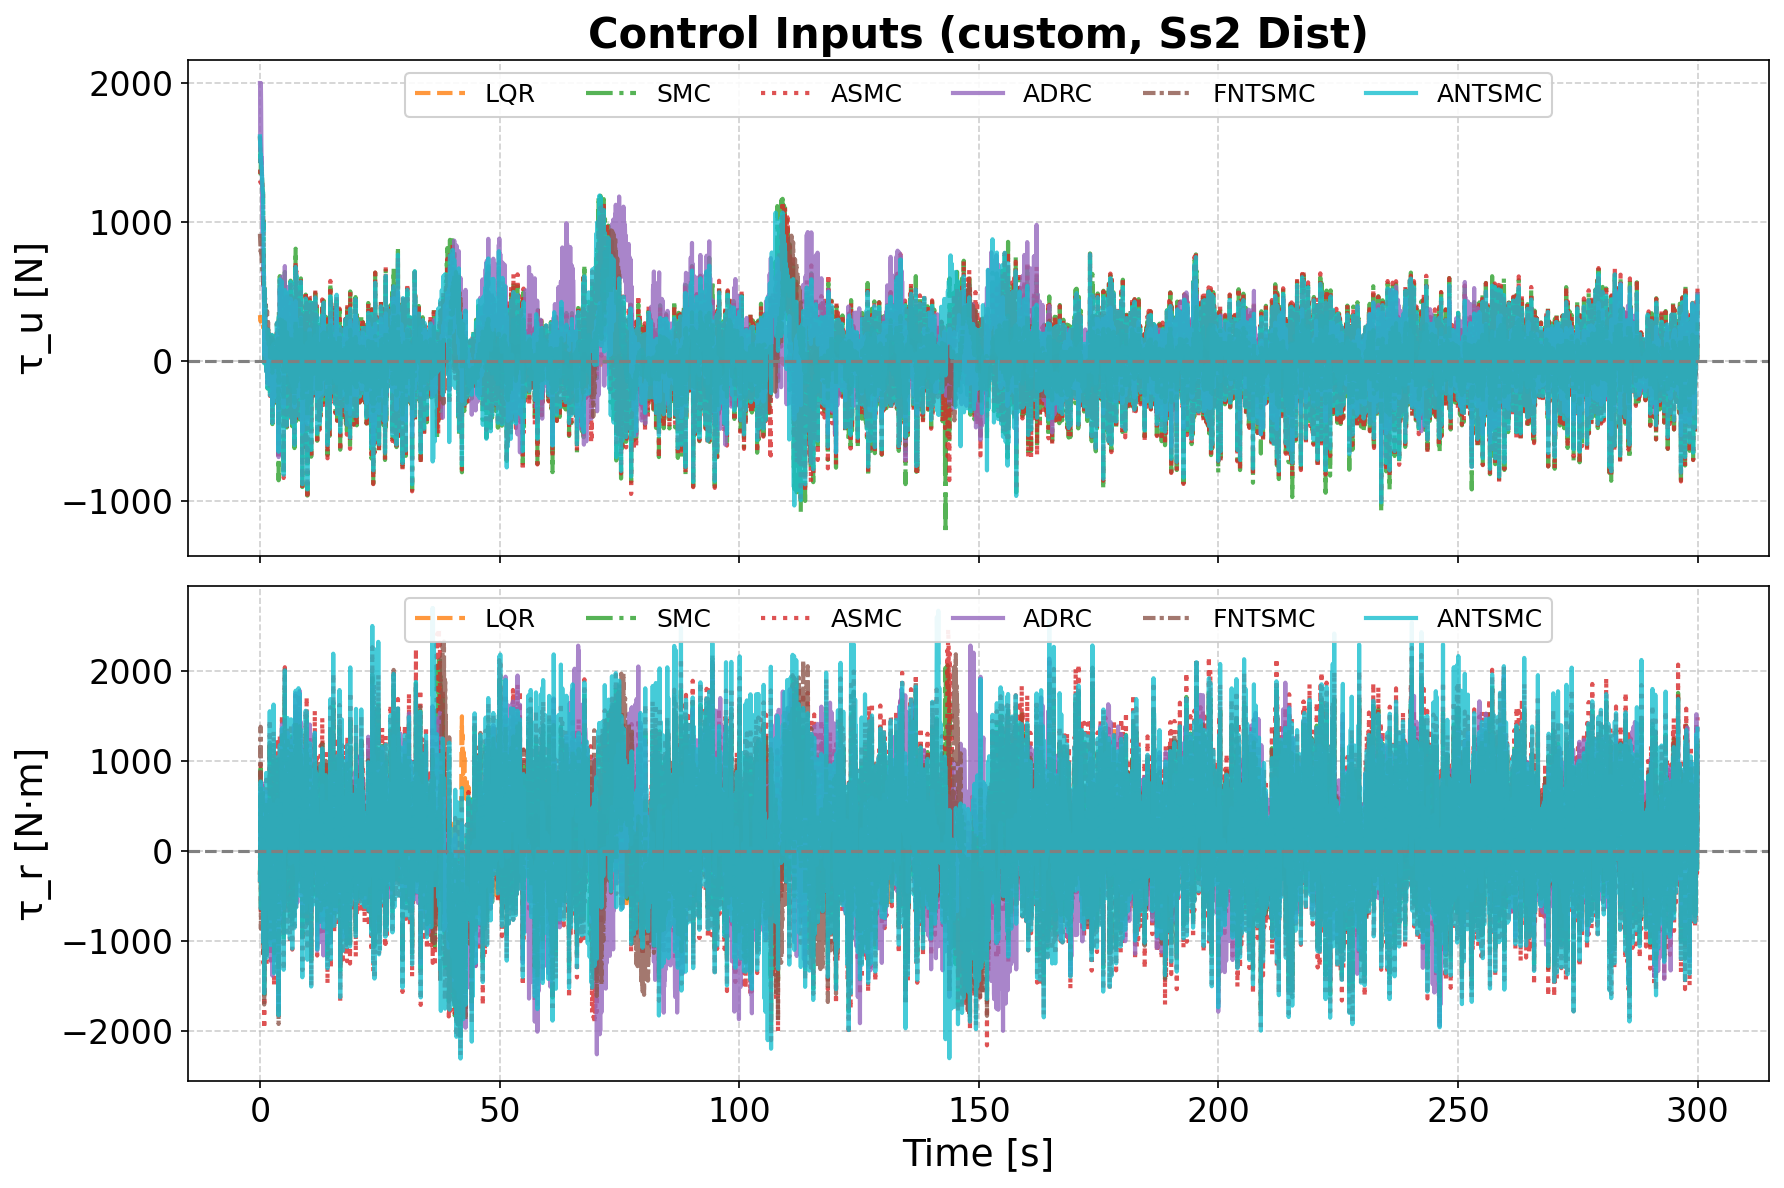
\includegraphics[width=\textwidth]{control_custom_ss2.png}
  \caption{Custom path.}
\end{subfigure}\hfill
\begin{subfigure}[b]{0.48\textwidth}
  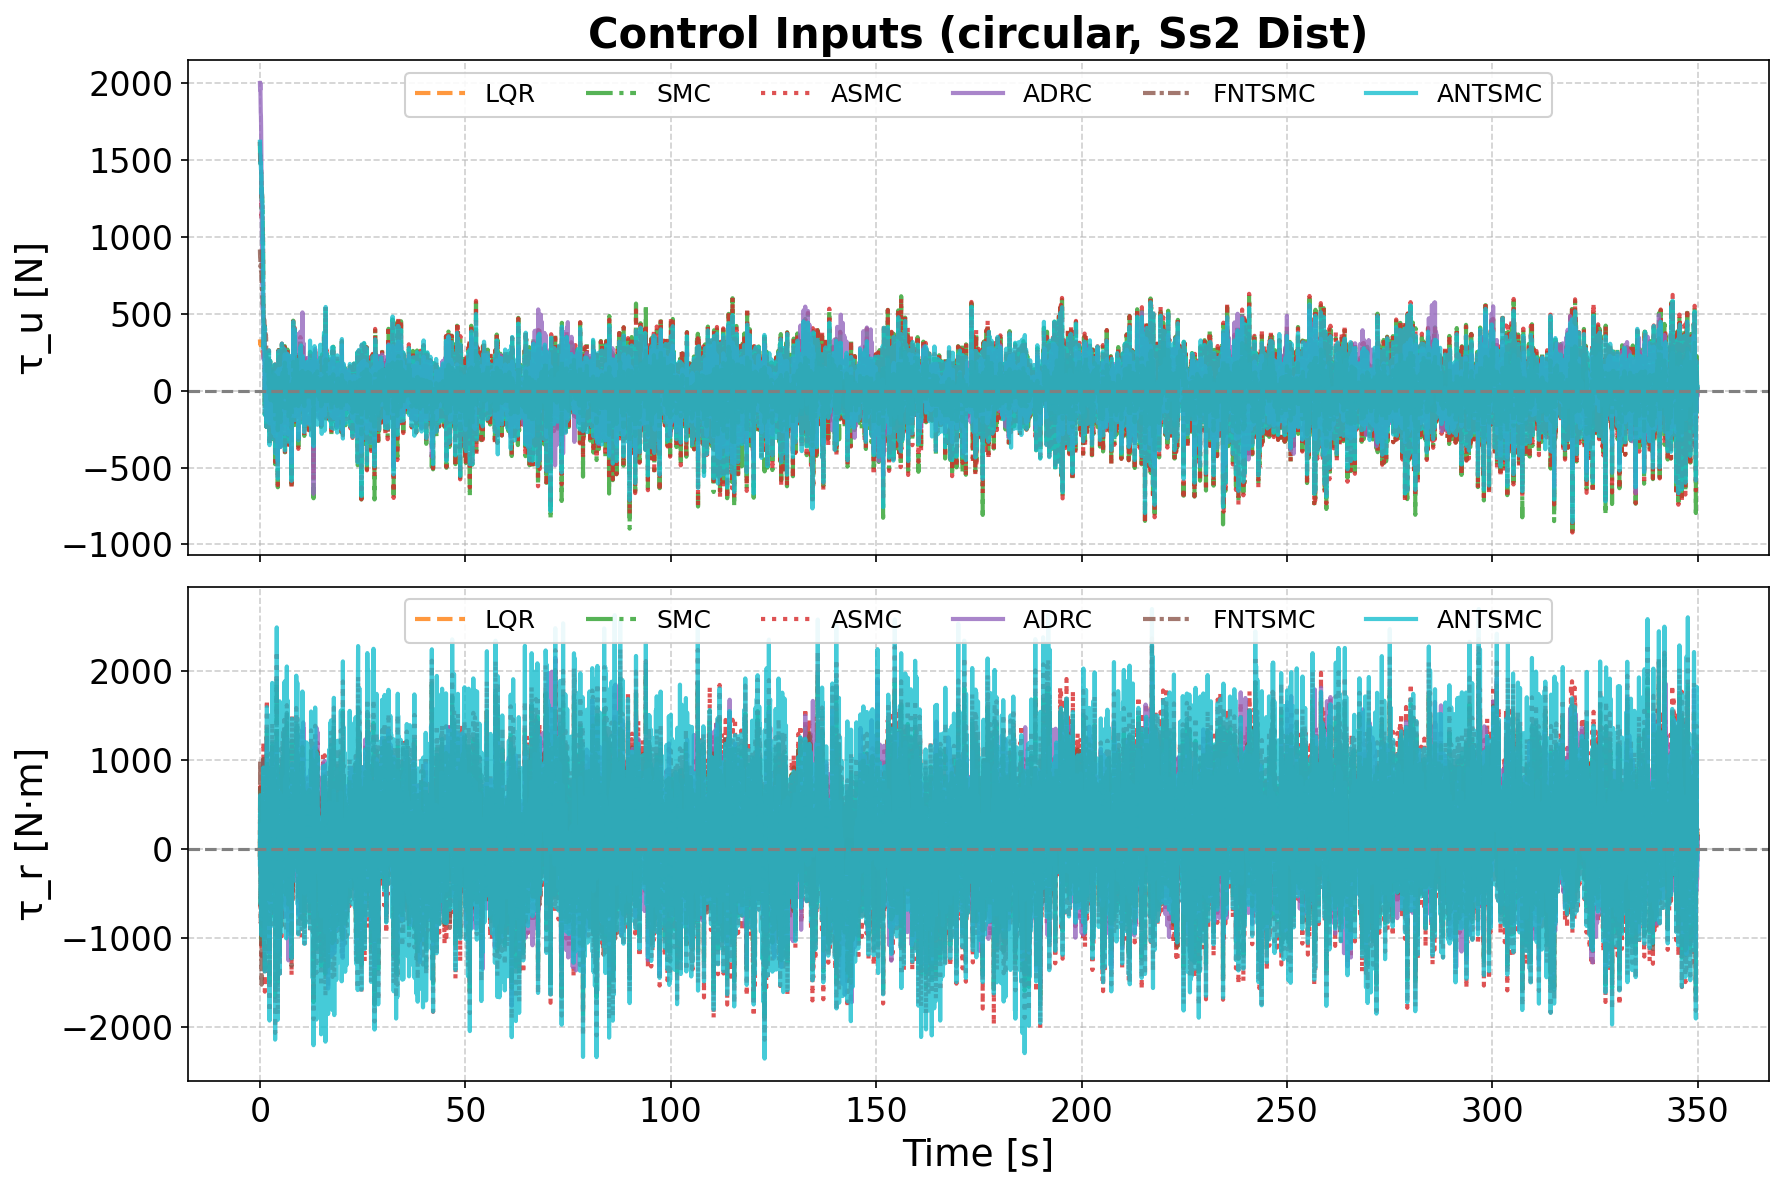
\includegraphics[width=\textwidth]{control_circular_ss2.png}
  \caption{Circular path.}
\end{subfigure}\\[6pt]
\begin{subfigure}[b]{0.48\textwidth}
  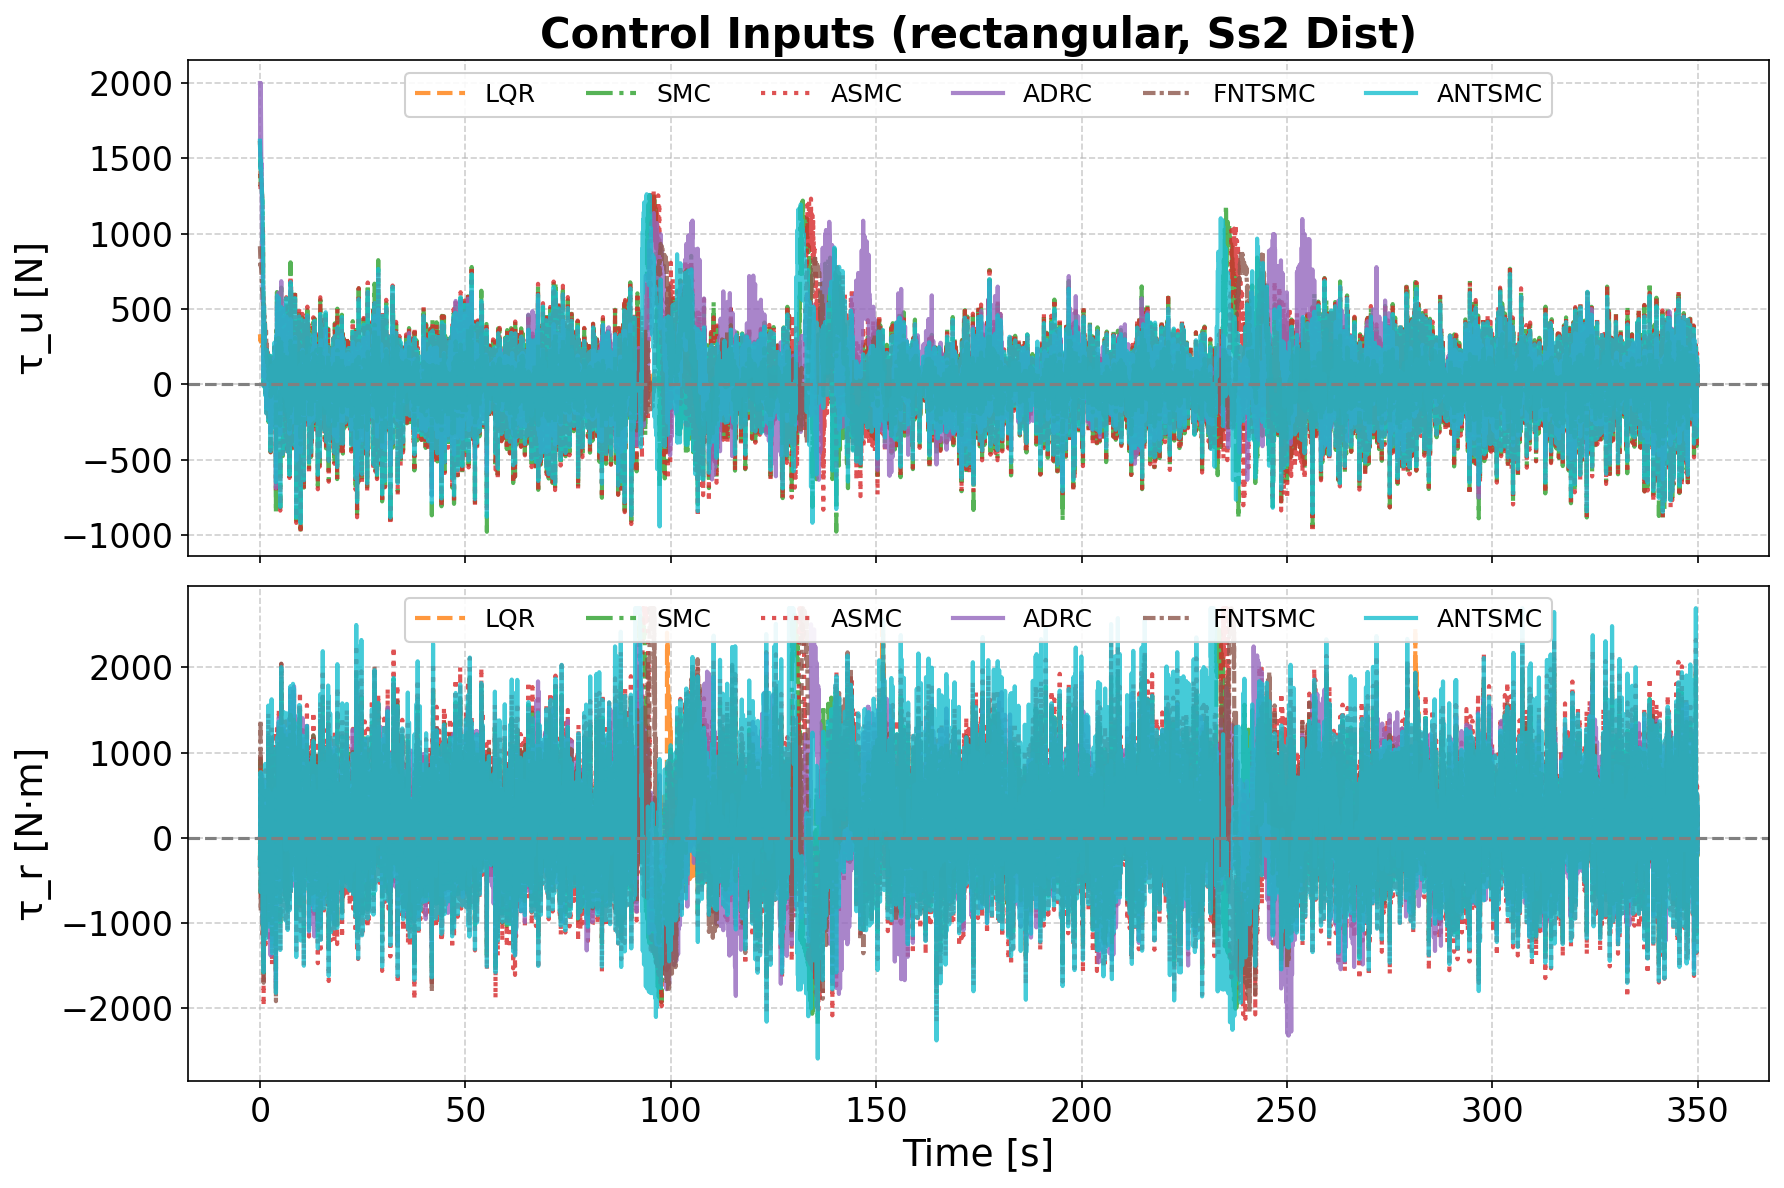
\includegraphics[width=\textwidth]{control_rectangular_ss2.png}
  \caption{Rectangular path.}
\end{subfigure}\hfill
\begin{subfigure}[b]{0.48\textwidth}
  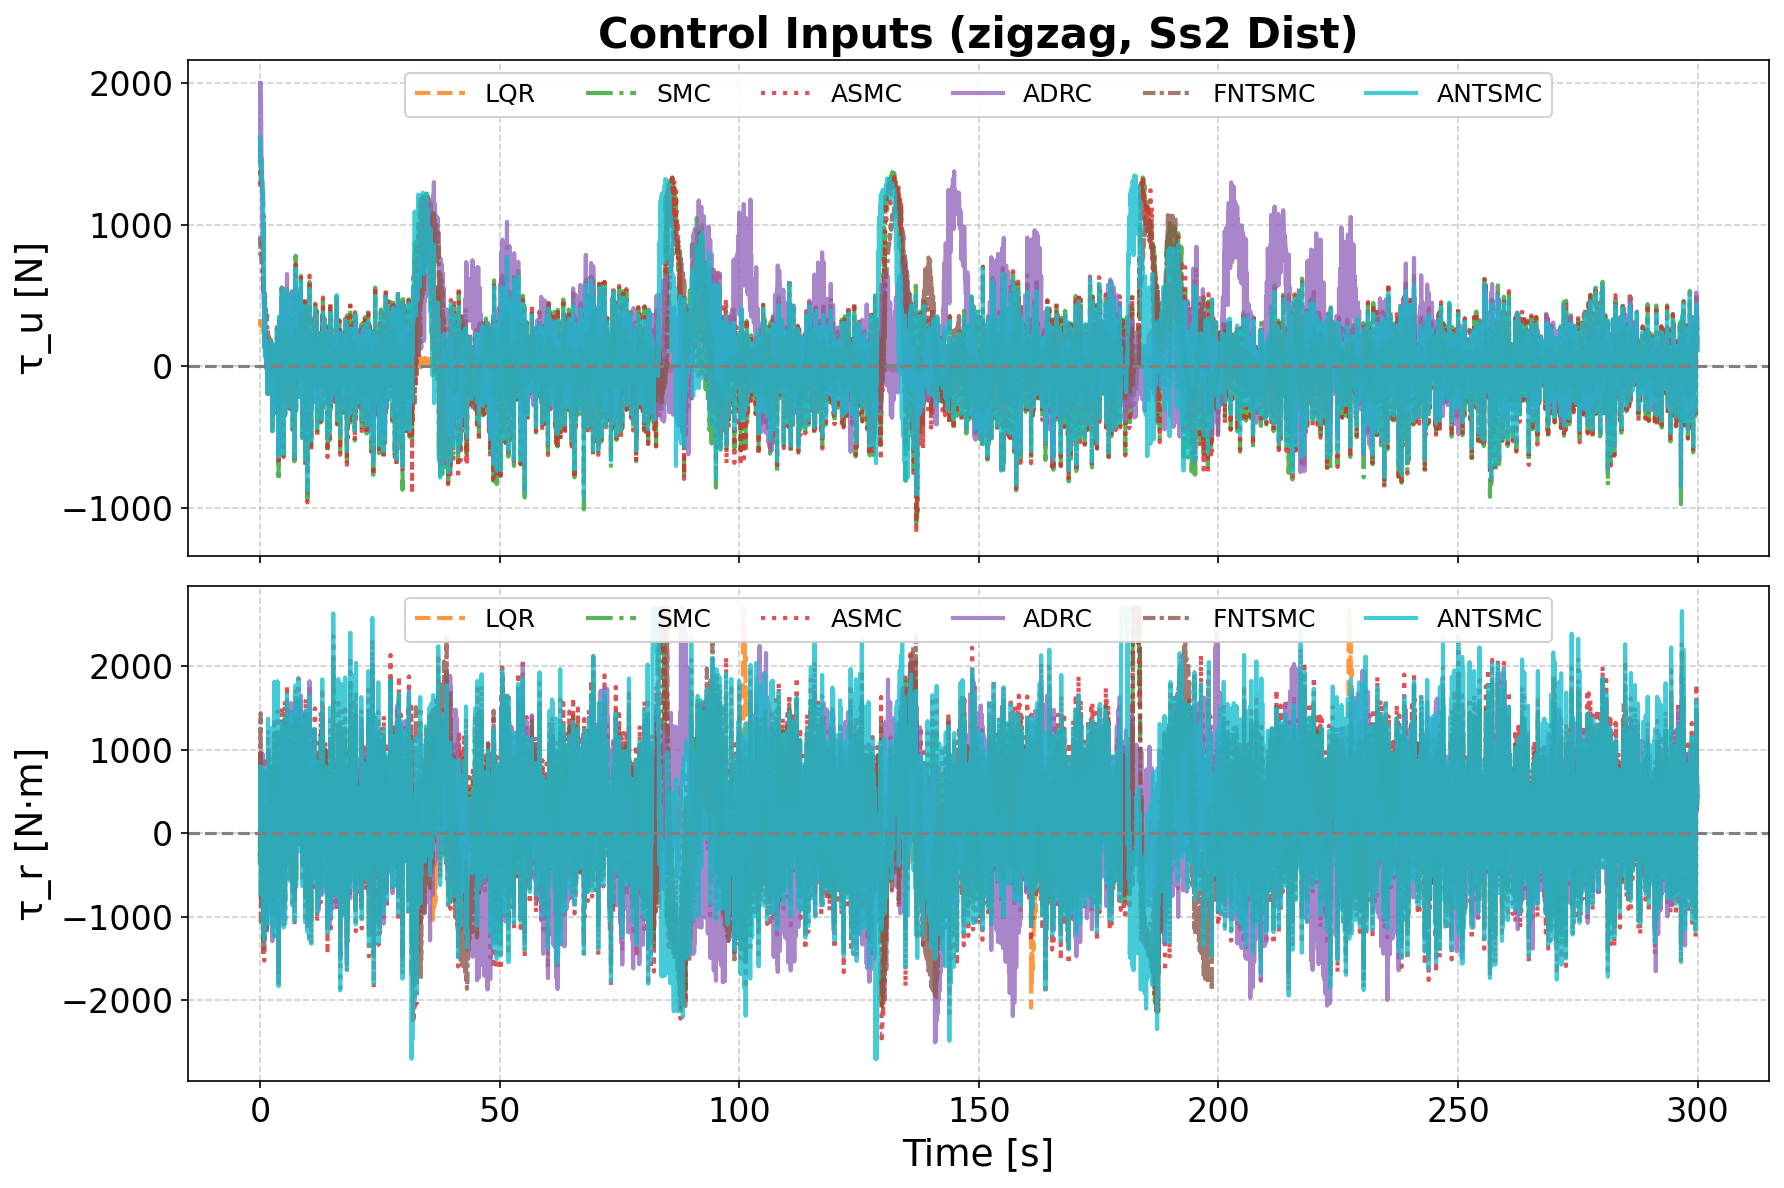
\includegraphics[width=\textwidth]{control_zigzag_ss2.png}
  \caption{Zigzag path.}
\end{subfigure}
\caption{Control effort ($\tau_u$, $\tau_r$) at Sea State~2 for all four paths. ANTSMC's adaptive gain increases for additional robustness.}
\label{fig:ctrl_ss2}
\end{figure*}

\subsubsection{RMS Bar Chart --- SS\,2}

\begin{figure}[t]
\centering
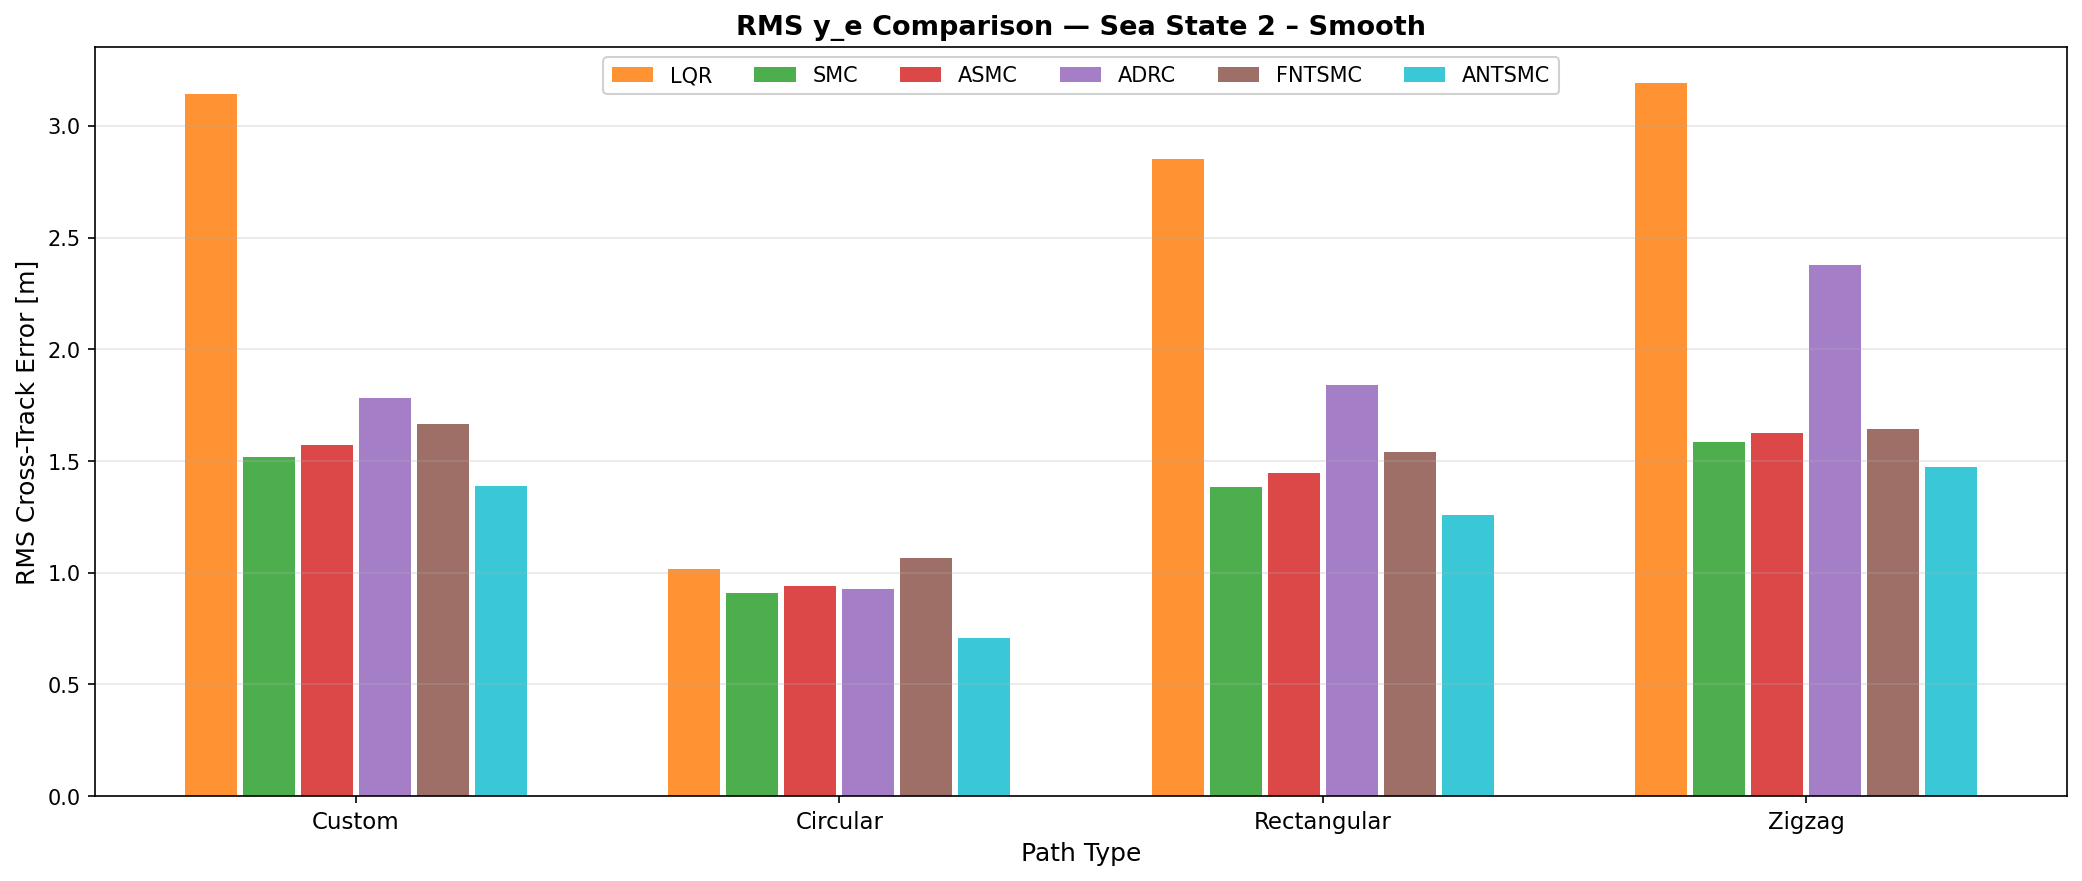
\includegraphics[width=\columnwidth]{bar_rms_ye_ss2.png}
\caption{RMS cross-track error bar chart at Sea State~2. ANTSMC achieves the lowest bars across all paths.}
\label{fig:bar_ss2}
\end{figure}


\subsection{Sea State 3 --- Slight ($\alpha_s = 0.60$)}

Under the strongest tested disturbances (Table~\ref{tab:ss3}), \textbf{ANTSMC maintains its lead}: RMS $y_e = 1.947$~m, an 8.1\% improvement over SMC (2.118~m) and 11.5\% over ADRC (2.200~m). ADRC performs well here thanks to properly tuned ESO bandwidth ($\omega_o = 3.5$--$4.0$~rad/s), closely rivalling SMC. ASMC (2.203~m) ties with ADRC, confirming the value of adaptive gain augmentation. FNTSMC drops to 5th place (2.551~m), as the FTDO's observer gain amplifies noise under strong disturbances, particularly at sharp path corners. The adaptive gain reaches $k_{s,r} \approx 0.8$--$1.0$ under persistent disturbance, automatically increasing robustness.

\textbf{Ranking (SS\,3):} \#1 ANTSMC, \#2 SMC, \#3 ADRC, \#4 ASMC, \#5 FNTSMC, \#6 LQR.

\begin{table}[t]
\centering
\caption{Sea State 3 (Slight) --- cross-path average steady-state performance. Best values in \textbf{bold}.}
\label{tab:ss3}
\begin{tabular}{lccccc}
\toprule
Controller & RMS $y_e$ [m] & Max $|y_e|$ [m] & RMS $\tau_u$ [N] & RMS $\tau_r$ [N\,m] & Energy \\
\midrule
LQR & 4.091 & 10.162 & 77.2 & 400.4 & 48\,946 \\
SMC & 2.118 & 4.338 & 376.8 & 734.7 & 176\,440 \\
ASMC & 2.203 & 4.395 & 371.7 & 827.7 & 176\,339 \\
ADRC & 2.200 & 5.828 & 313.9 & 726.8 & 162\,765 \\
FNTSMC & 2.551 & 5.431 & 275.7 & 780.2 & 134\,316 \\
\textbf{ANTSMC} & \textbf{1.947} & \textbf{4.462} & 351.2 & 810.5 & 168\,829 \\
\bottomrule
\end{tabular}
\end{table}

\subsubsection{Trajectory Tracking at SS\,3}

Fig.~\ref{fig:traj_ss3} shows trajectory tracking at the most challenging sea state. ANTSMC achieves clearly visible trajectory superiority on all paths. The custom path (a) shows ANTSMC at 2.171~m RMS---the lowest among all controllers. The rectangular path (c) demonstrates the effectiveness of the error-proportional leakage at preventing integral windup during large sway excursions at $90^\circ$ corners under strong disturbances. FNTSMC exhibits the largest overshoots among the sliding-mode controllers, as the FTDO struggles to distinguish external disturbances from the controller's own commanded dynamics at sharp transitions.

\begin{figure*}[t]
\centering
\begin{subfigure}[b]{0.48\textwidth}
  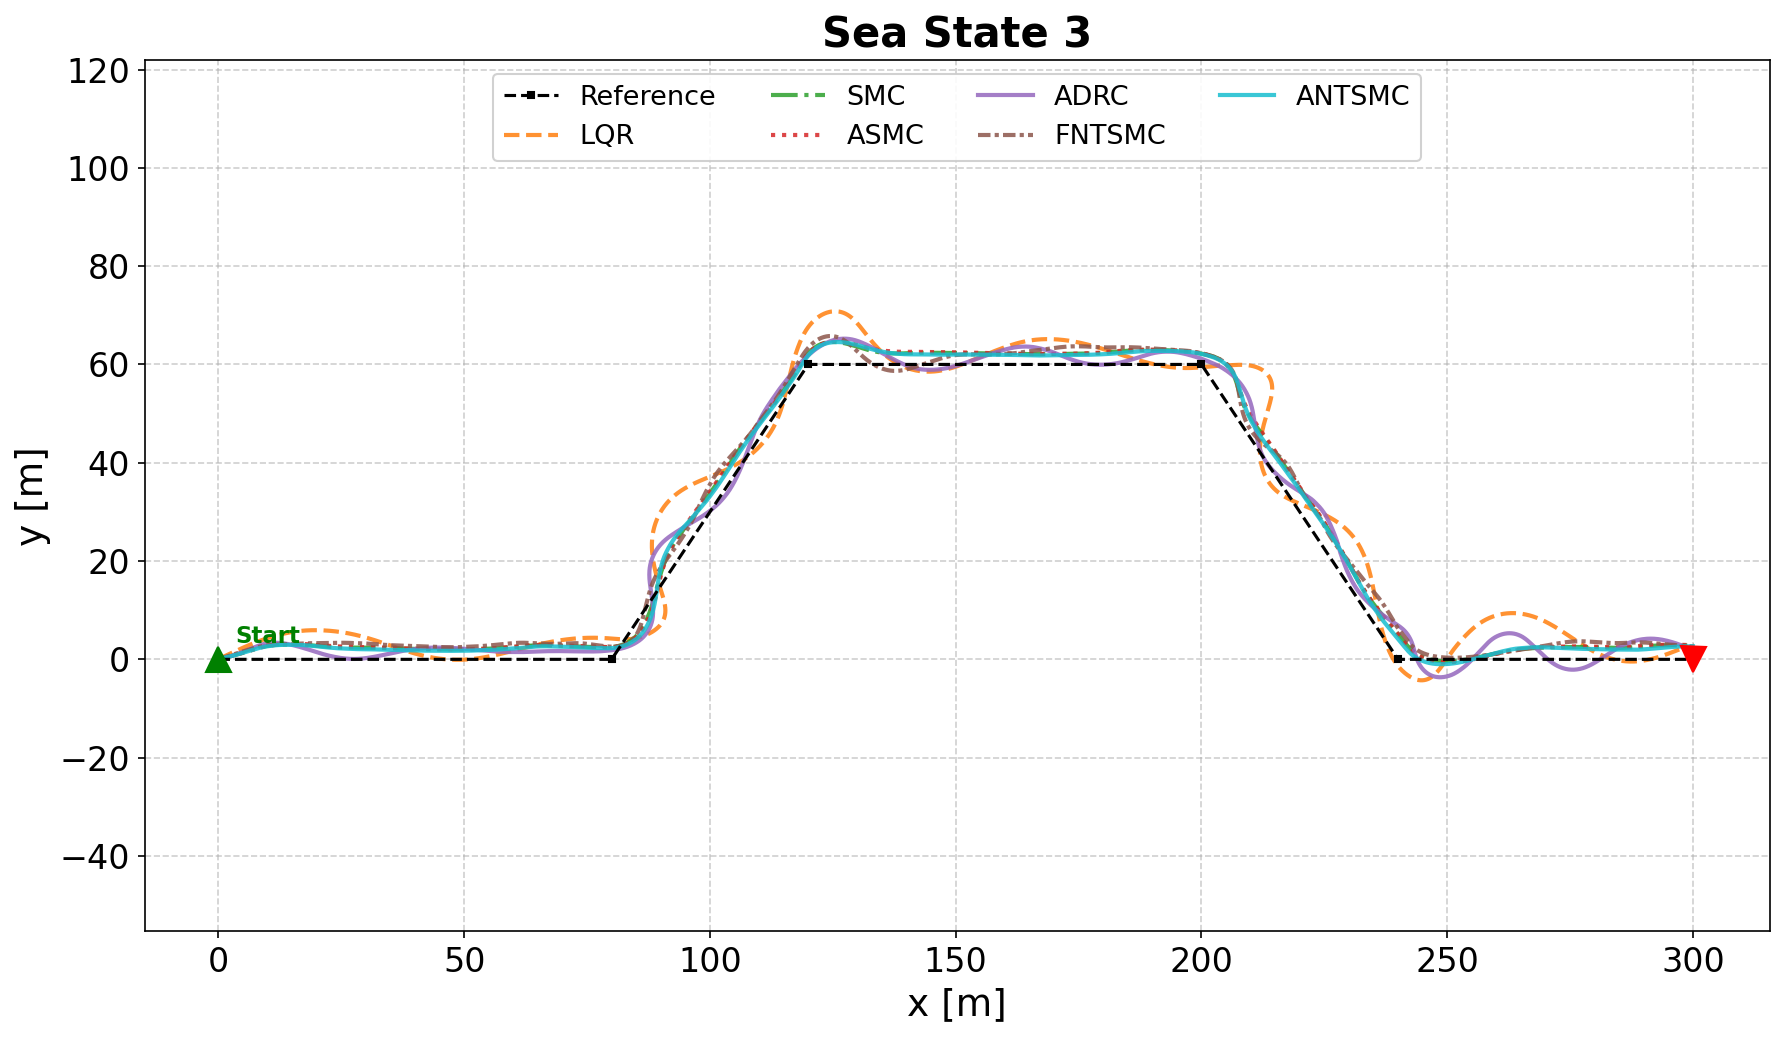
\includegraphics[width=\textwidth]{traj_custom_ss3.png}
  \caption{Custom path.}
\end{subfigure}\hfill
\begin{subfigure}[b]{0.48\textwidth}
  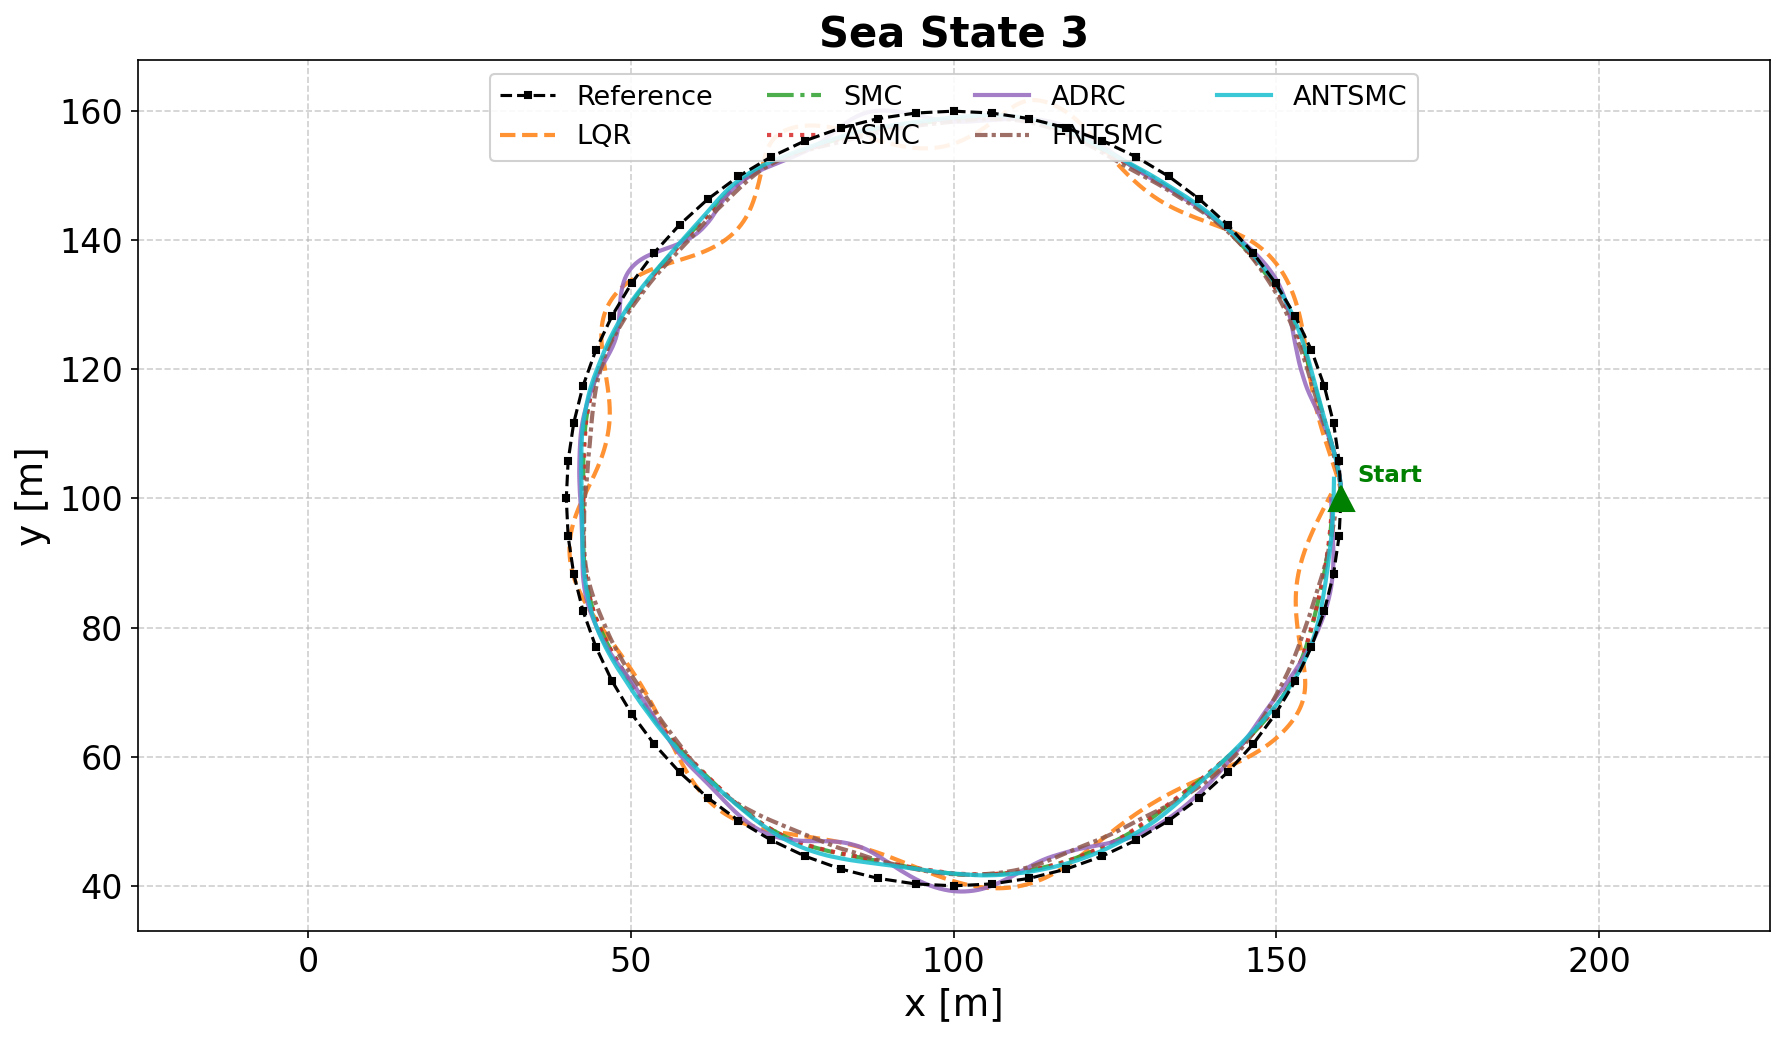
\includegraphics[width=\textwidth]{traj_circular_ss3.png}
  \caption{Circular path.}
\end{subfigure}\\[6pt]
\begin{subfigure}[b]{0.48\textwidth}
  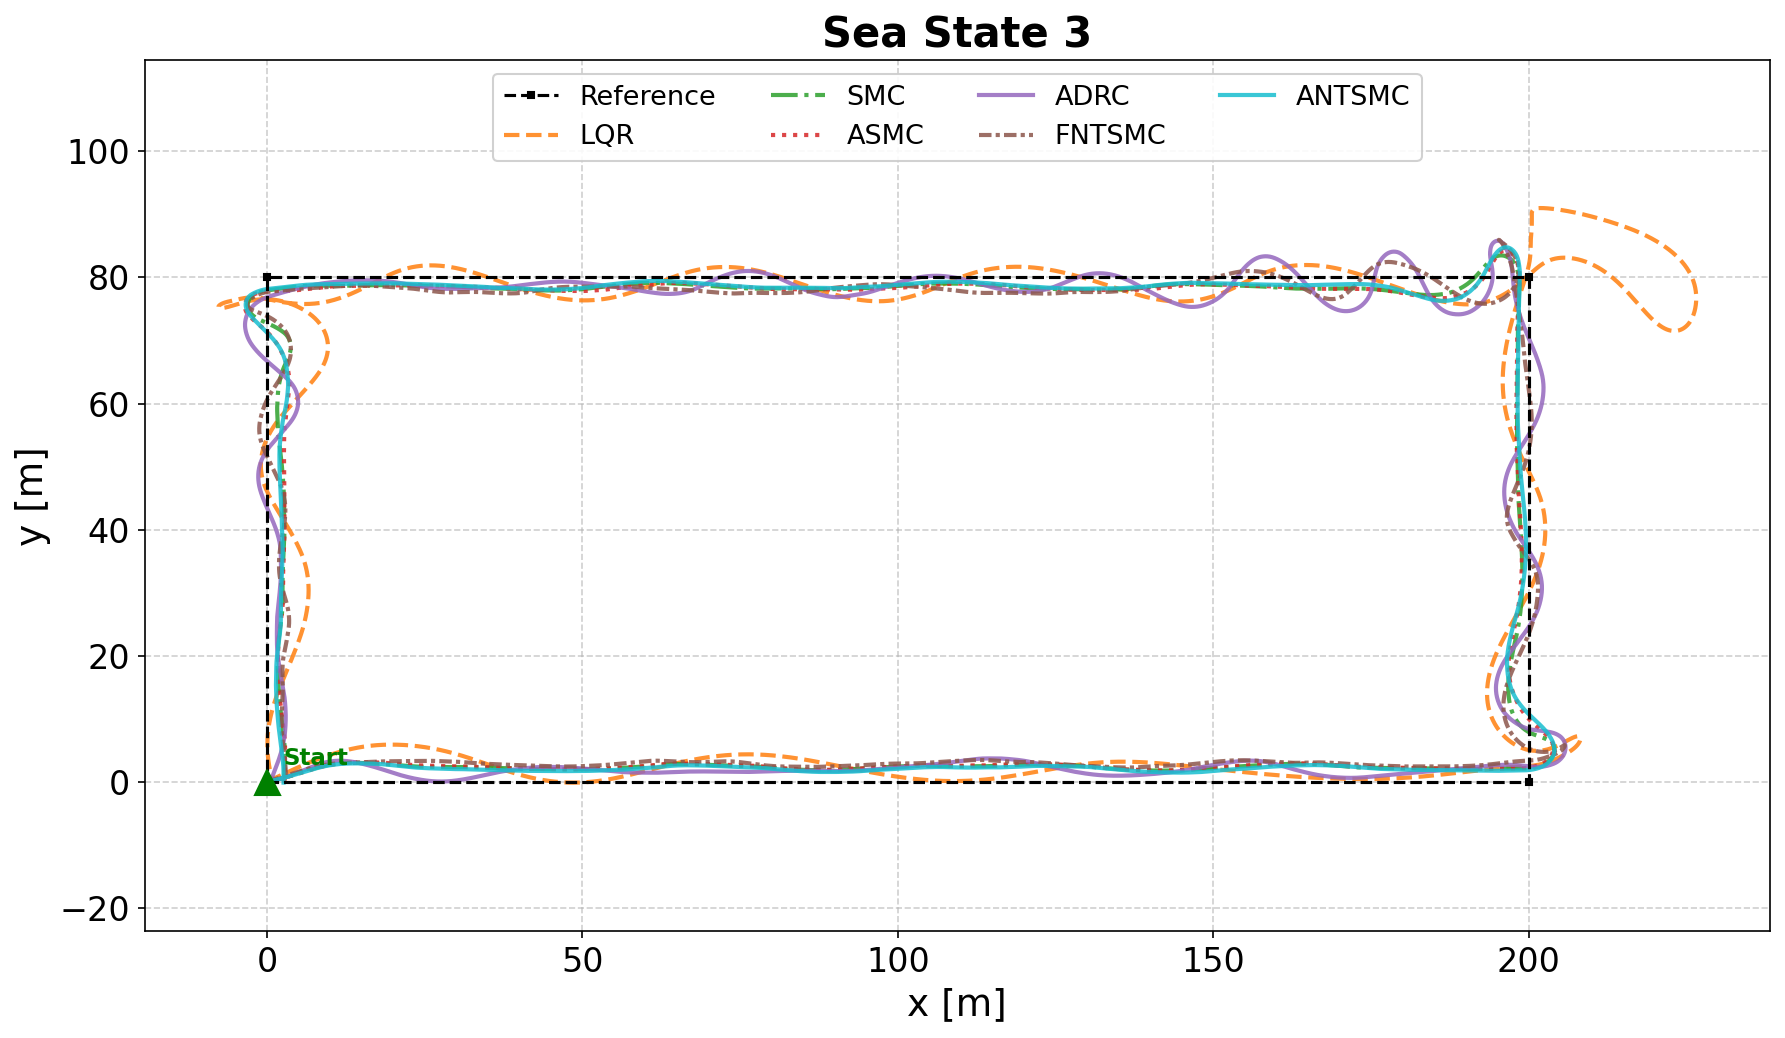
\includegraphics[width=\textwidth]{traj_rectangular_ss3.png}
  \caption{Rectangular path.}
\end{subfigure}\hfill
\begin{subfigure}[b]{0.48\textwidth}
  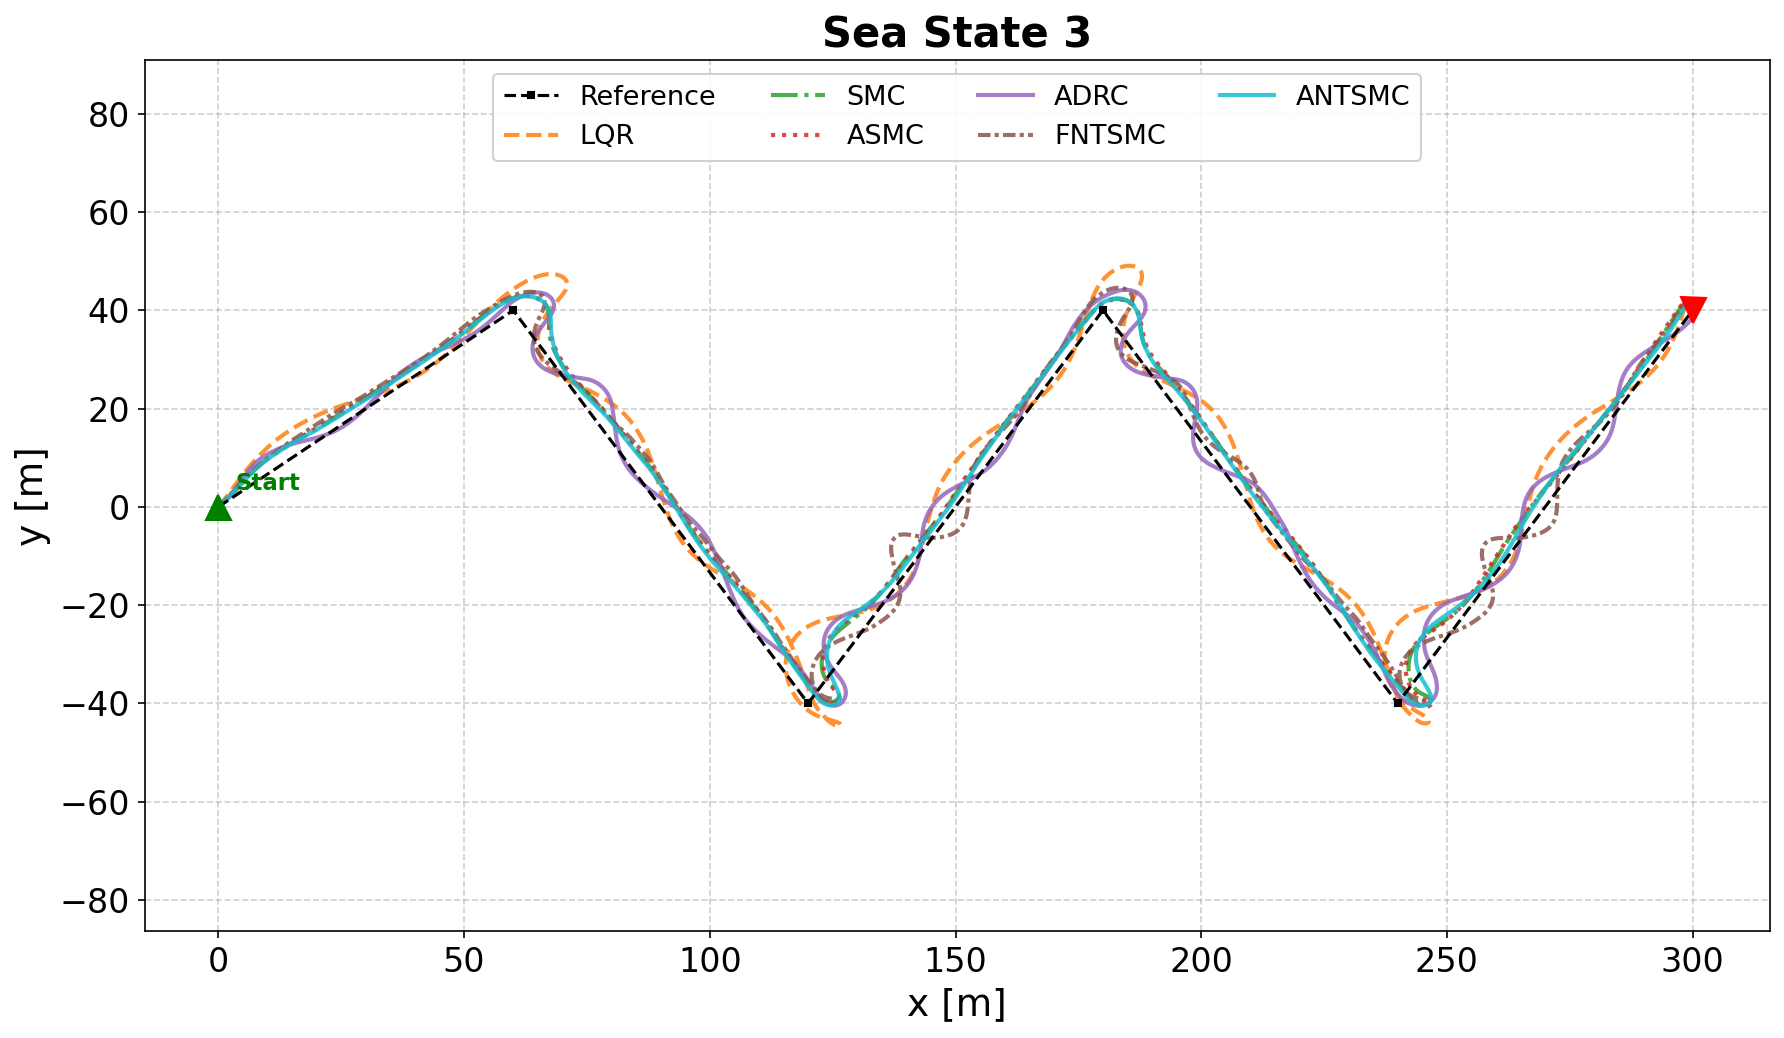
\includegraphics[width=\textwidth]{traj_zigzag_ss3.png}
  \caption{Zigzag path.}
\end{subfigure}
\caption{Trajectory tracking at Sea State~3 for all four path geometries. ANTSMC maintains clear trajectory superiority under the strongest disturbances. The gap between nonlinear controllers and linear ones is most pronounced.}
\label{fig:traj_ss3}
\end{figure*}

\subsubsection{Cross-Track Error at SS\,3}

Fig.~\ref{fig:ye_ss3} shows the cross-track error at SS\,3. ANTSMC achieves the tightest envelope on every path, with 1.407~m on the circular path (b) closely followed by ADRC (1.498~m) which benefits from its well-tuned ESO on this smooth geometry. The zigzag path (d) is the ultimate stress test: ANTSMC achieves 2.212~m versus SMC's 2.356~m. FNTSMC's FTDO-induced overshoots are most visible on the rectangular and zigzag paths, increasing its average to 2.551~m---above even ADRC.

\begin{figure*}[t]
\centering
\begin{subfigure}[b]{0.48\textwidth}
  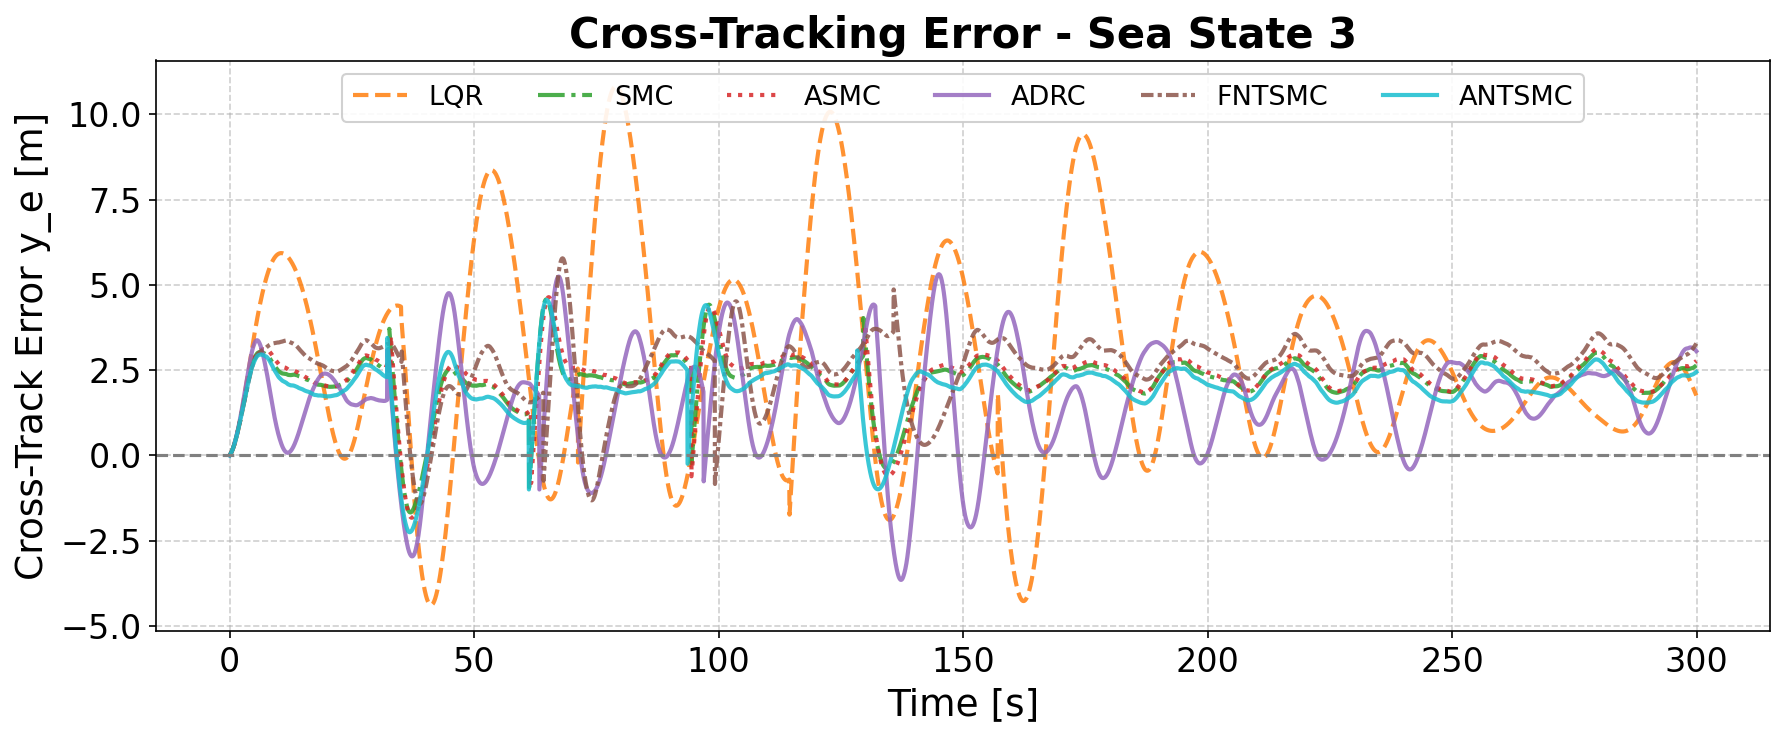
\includegraphics[width=\textwidth]{error_custom_ss3.png}
  \caption{Custom path.}
\end{subfigure}\hfill
\begin{subfigure}[b]{0.48\textwidth}
  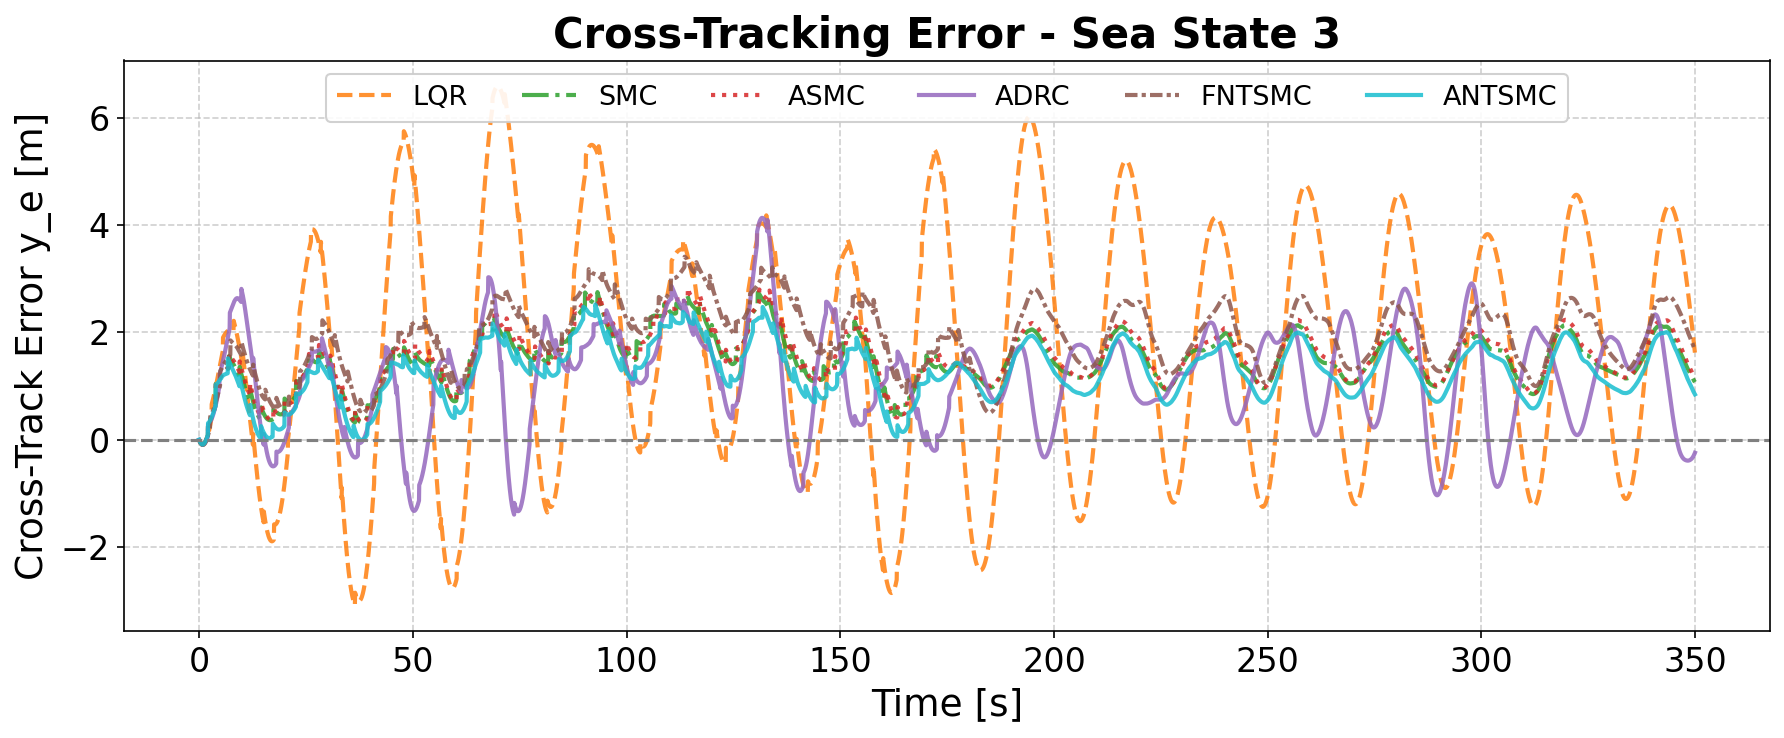
\includegraphics[width=\textwidth]{error_circular_ss3.png}
  \caption{Circular path.}
\end{subfigure}\\[6pt]
\begin{subfigure}[b]{0.48\textwidth}
  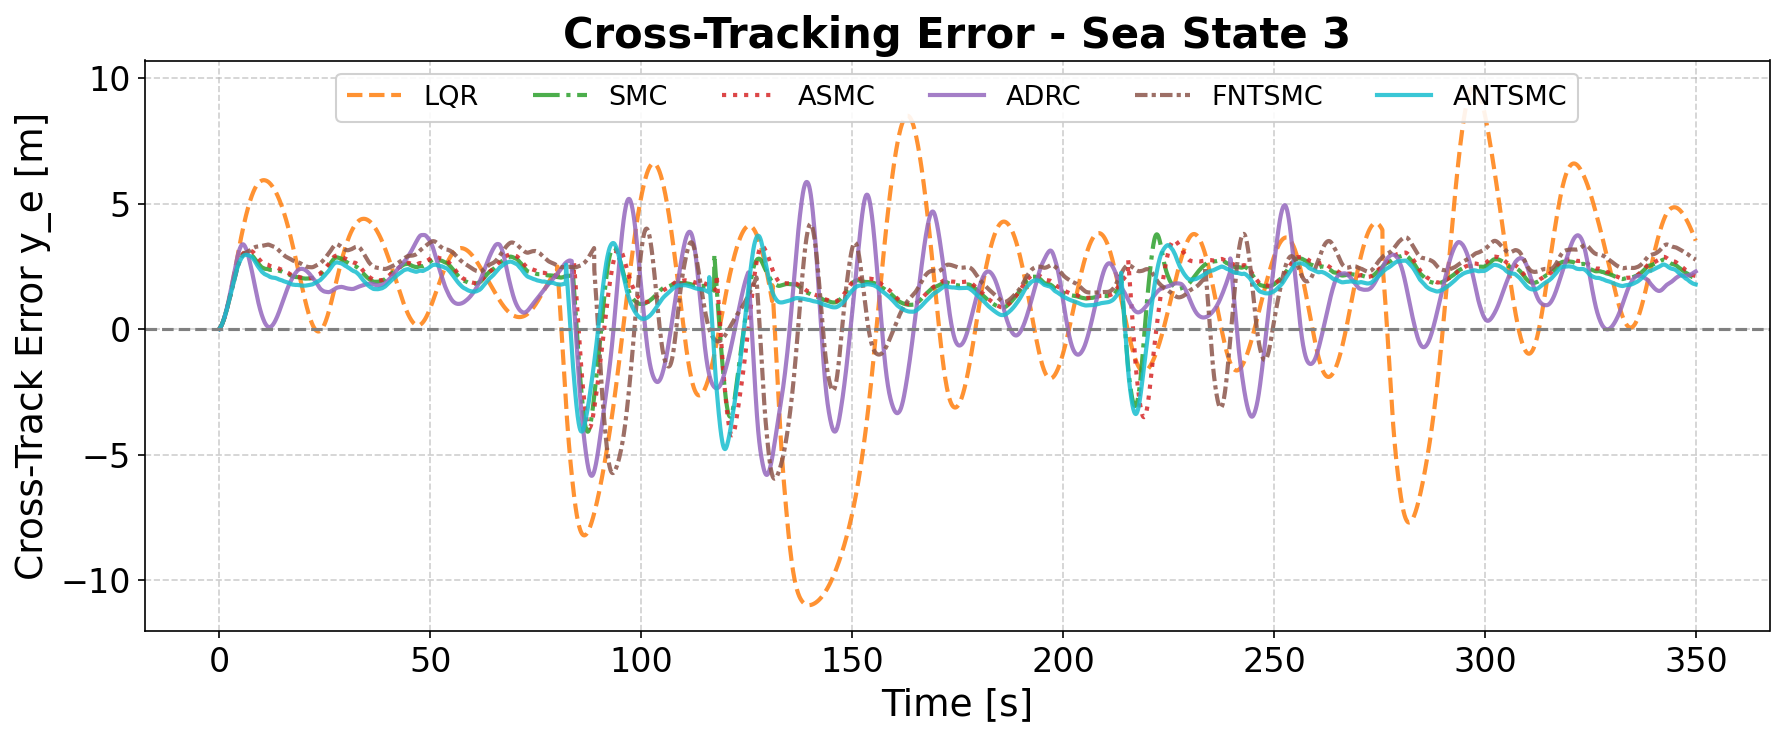
\includegraphics[width=\textwidth]{error_rectangular_ss3.png}
  \caption{Rectangular path.}
\end{subfigure}\hfill
\begin{subfigure}[b]{0.48\textwidth}
  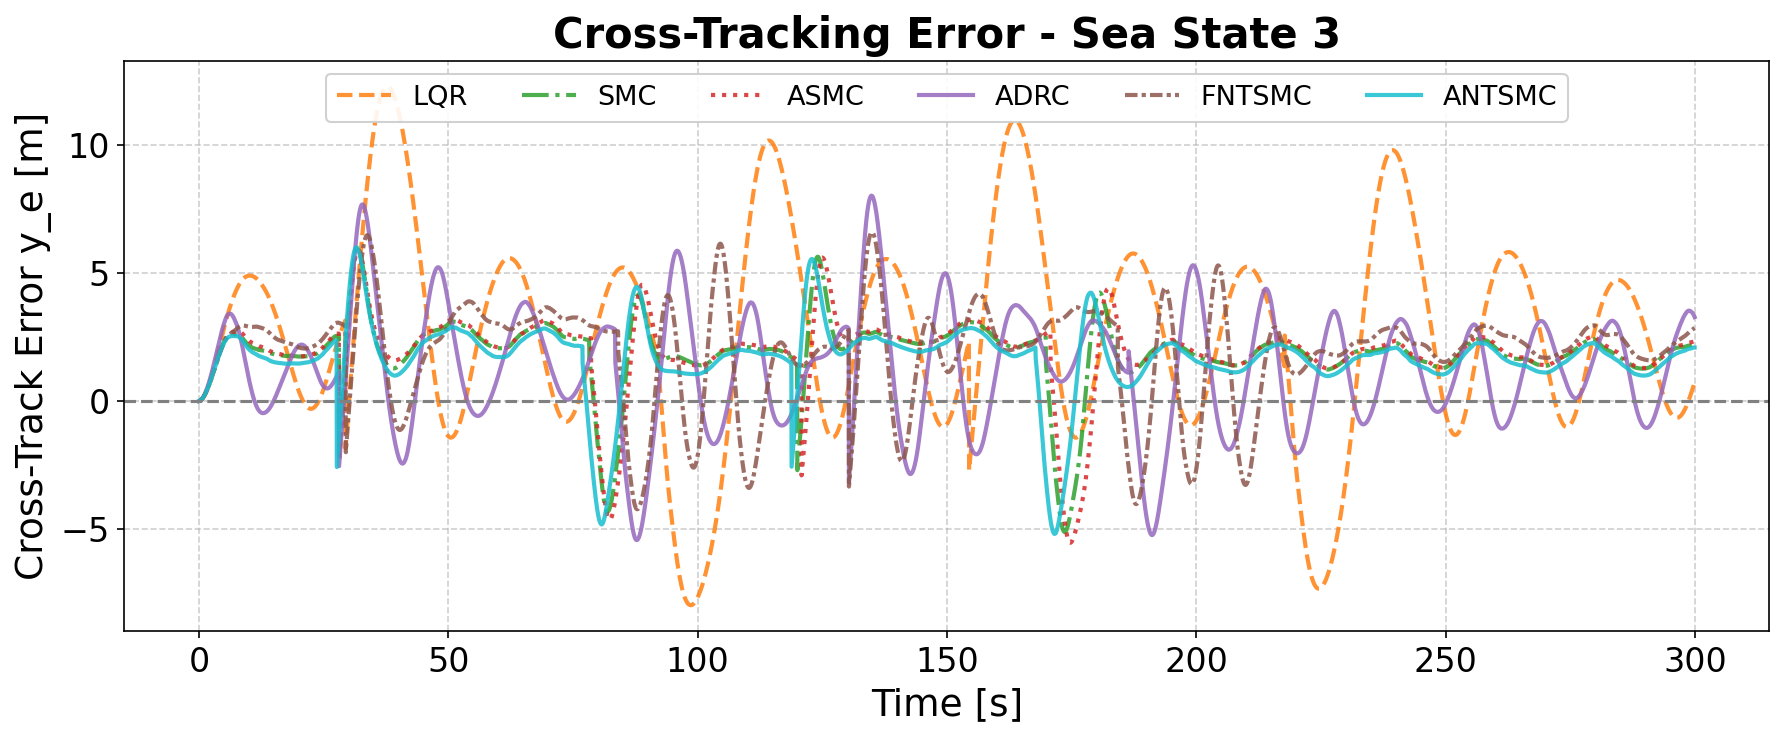
\includegraphics[width=\textwidth]{error_zigzag_ss3.png}
  \caption{Zigzag path.}
\end{subfigure}
\caption{Cross-track error $y_e(t)$ at Sea State~3 for all four paths. ANTSMC maintains the tightest error envelope under the strongest disturbances.}
\label{fig:ye_ss3}
\end{figure*}

\subsubsection{Heading Tracking at SS\,3}

Fig.~\ref{fig:heading_ss3} presents the heading responses at SS\,3. ADRC's ESO-induced heading lag at zigzag reversals (d) remains the controller's key weakness, a problem that cannot be resolved through bandwidth tuning alone. ANTSMC maintains responsive heading tracking.

\begin{figure*}[t]
\centering
\begin{subfigure}[b]{0.48\textwidth}
  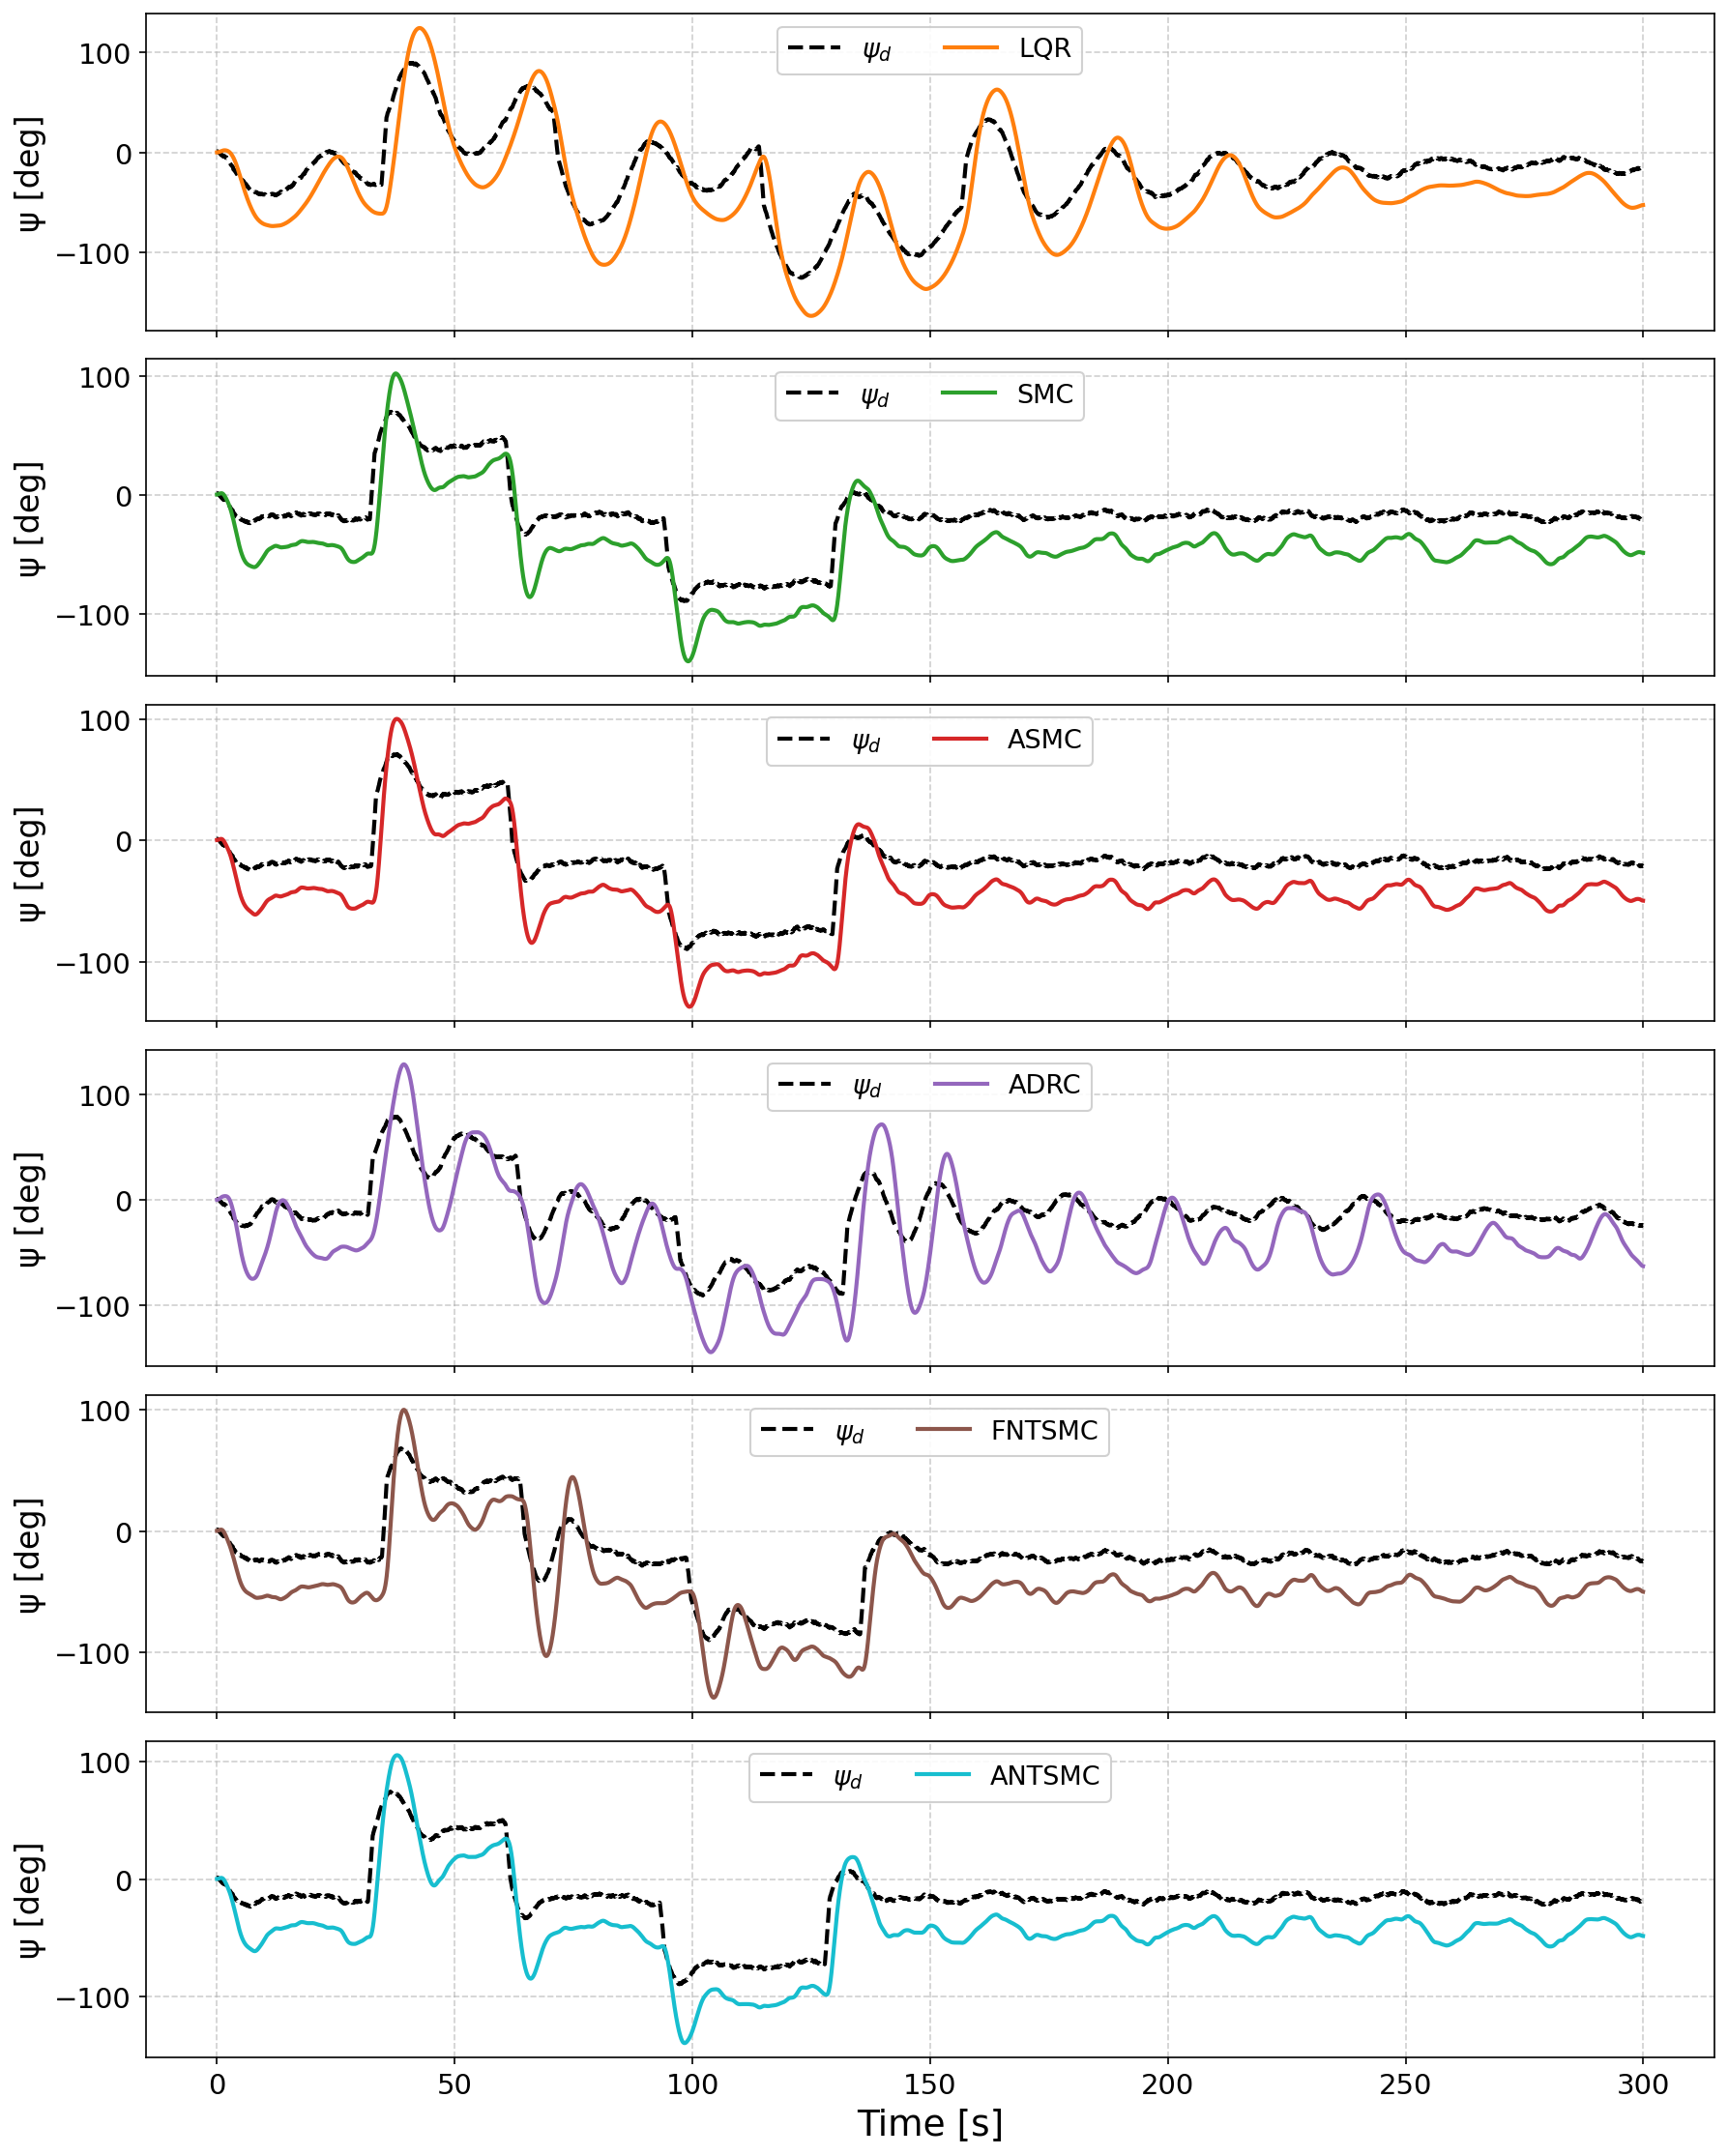
\includegraphics[width=\textwidth]{heading_custom_ss3.png}
  \caption{Custom path.}
\end{subfigure}\hfill
\begin{subfigure}[b]{0.48\textwidth}
  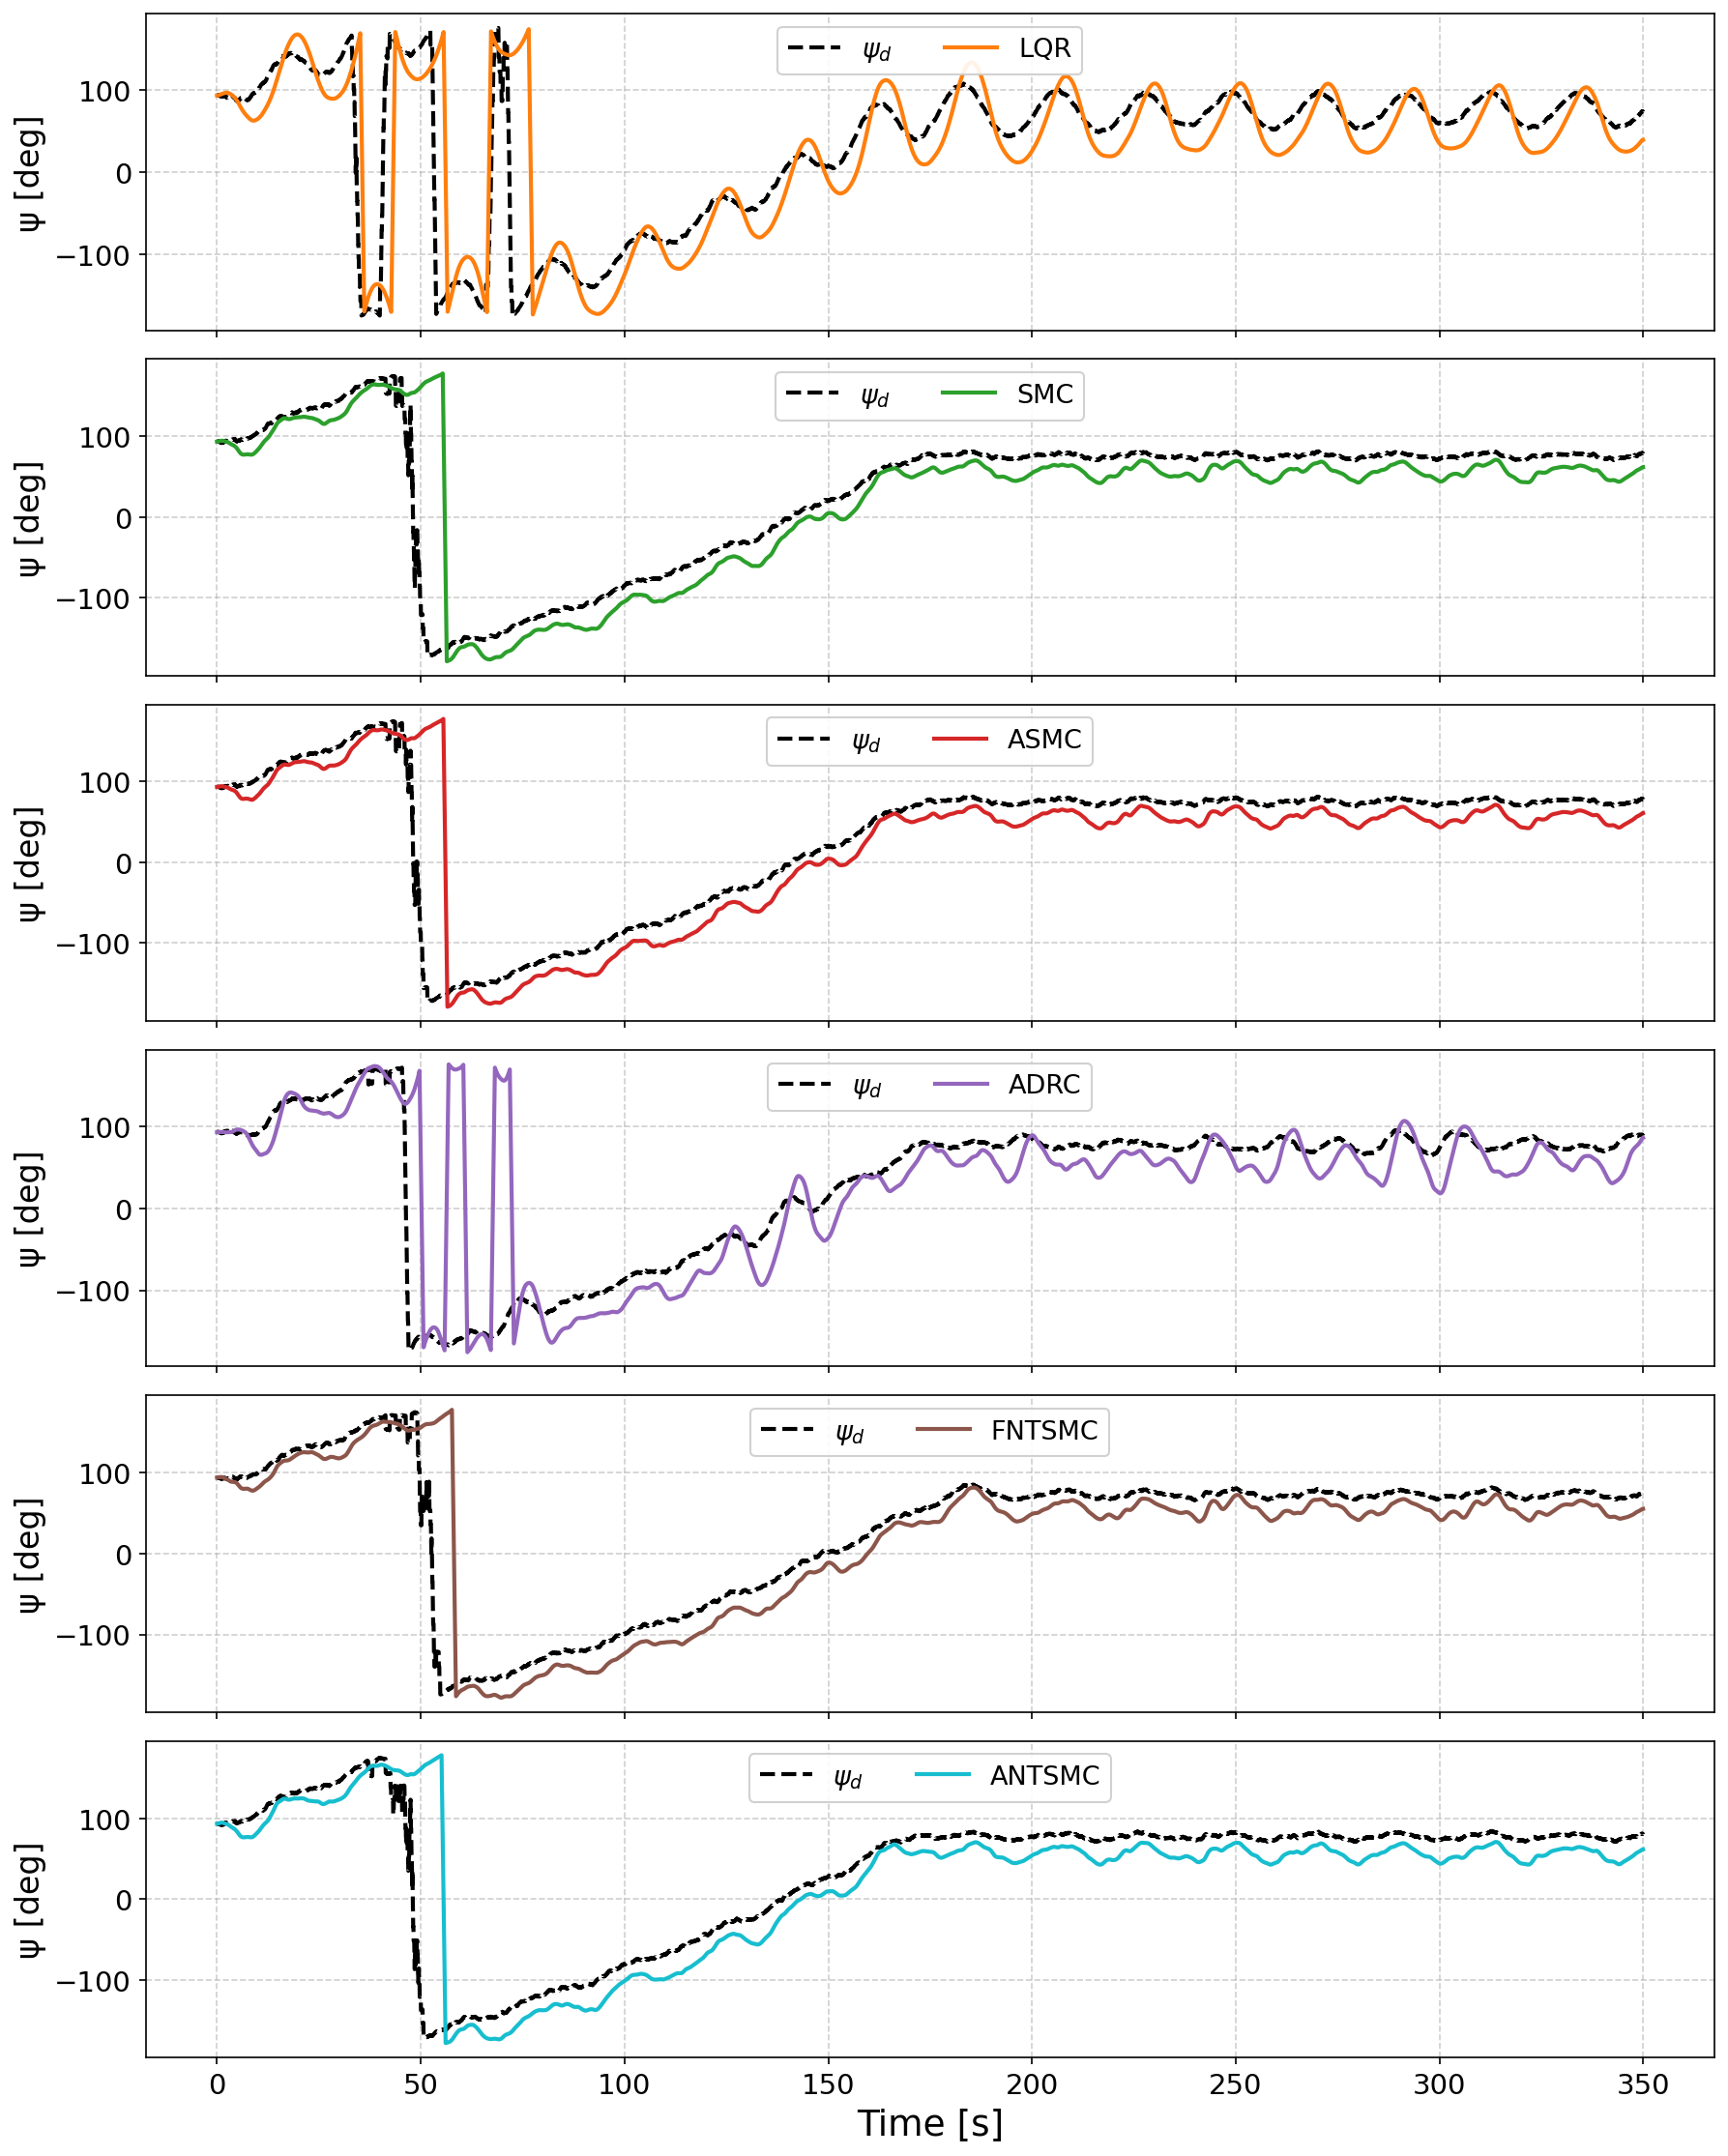
\includegraphics[width=\textwidth]{heading_circular_ss3.png}
  \caption{Circular path.}
\end{subfigure}\\[6pt]
\begin{subfigure}[b]{0.48\textwidth}
  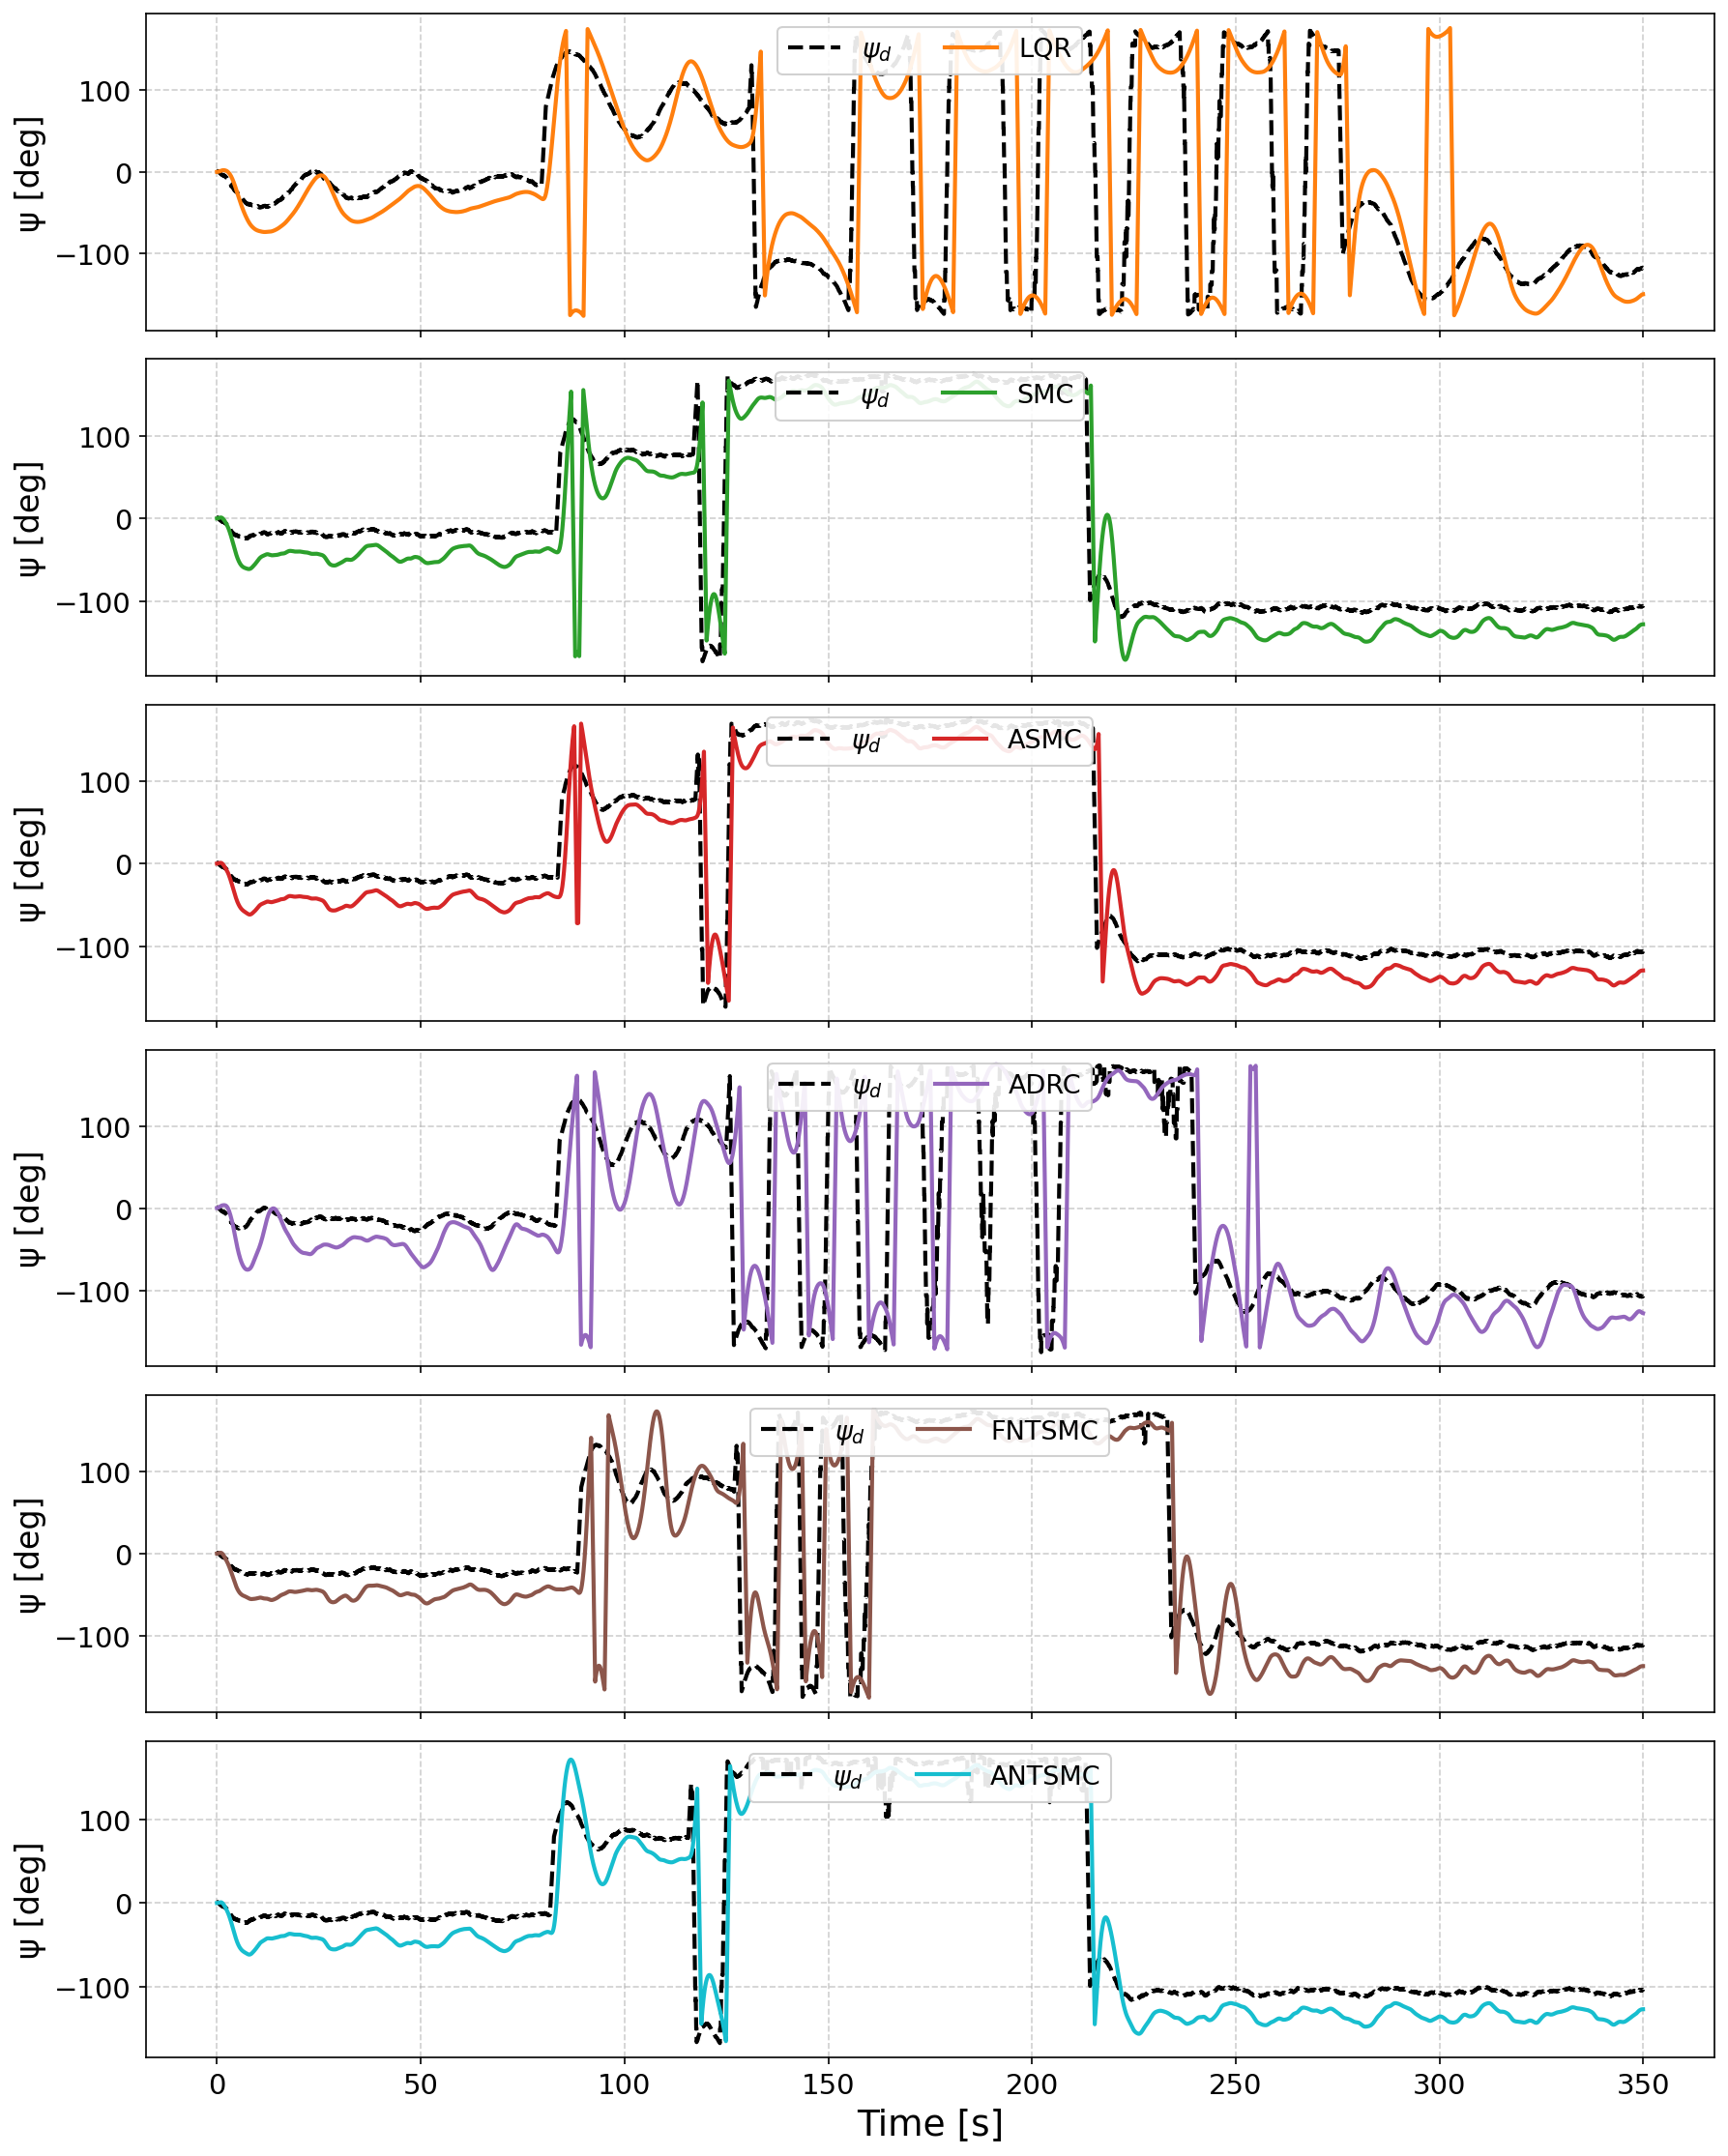
\includegraphics[width=\textwidth]{heading_rectangular_ss3.png}
  \caption{Rectangular path.}
\end{subfigure}\hfill
\begin{subfigure}[b]{0.48\textwidth}
  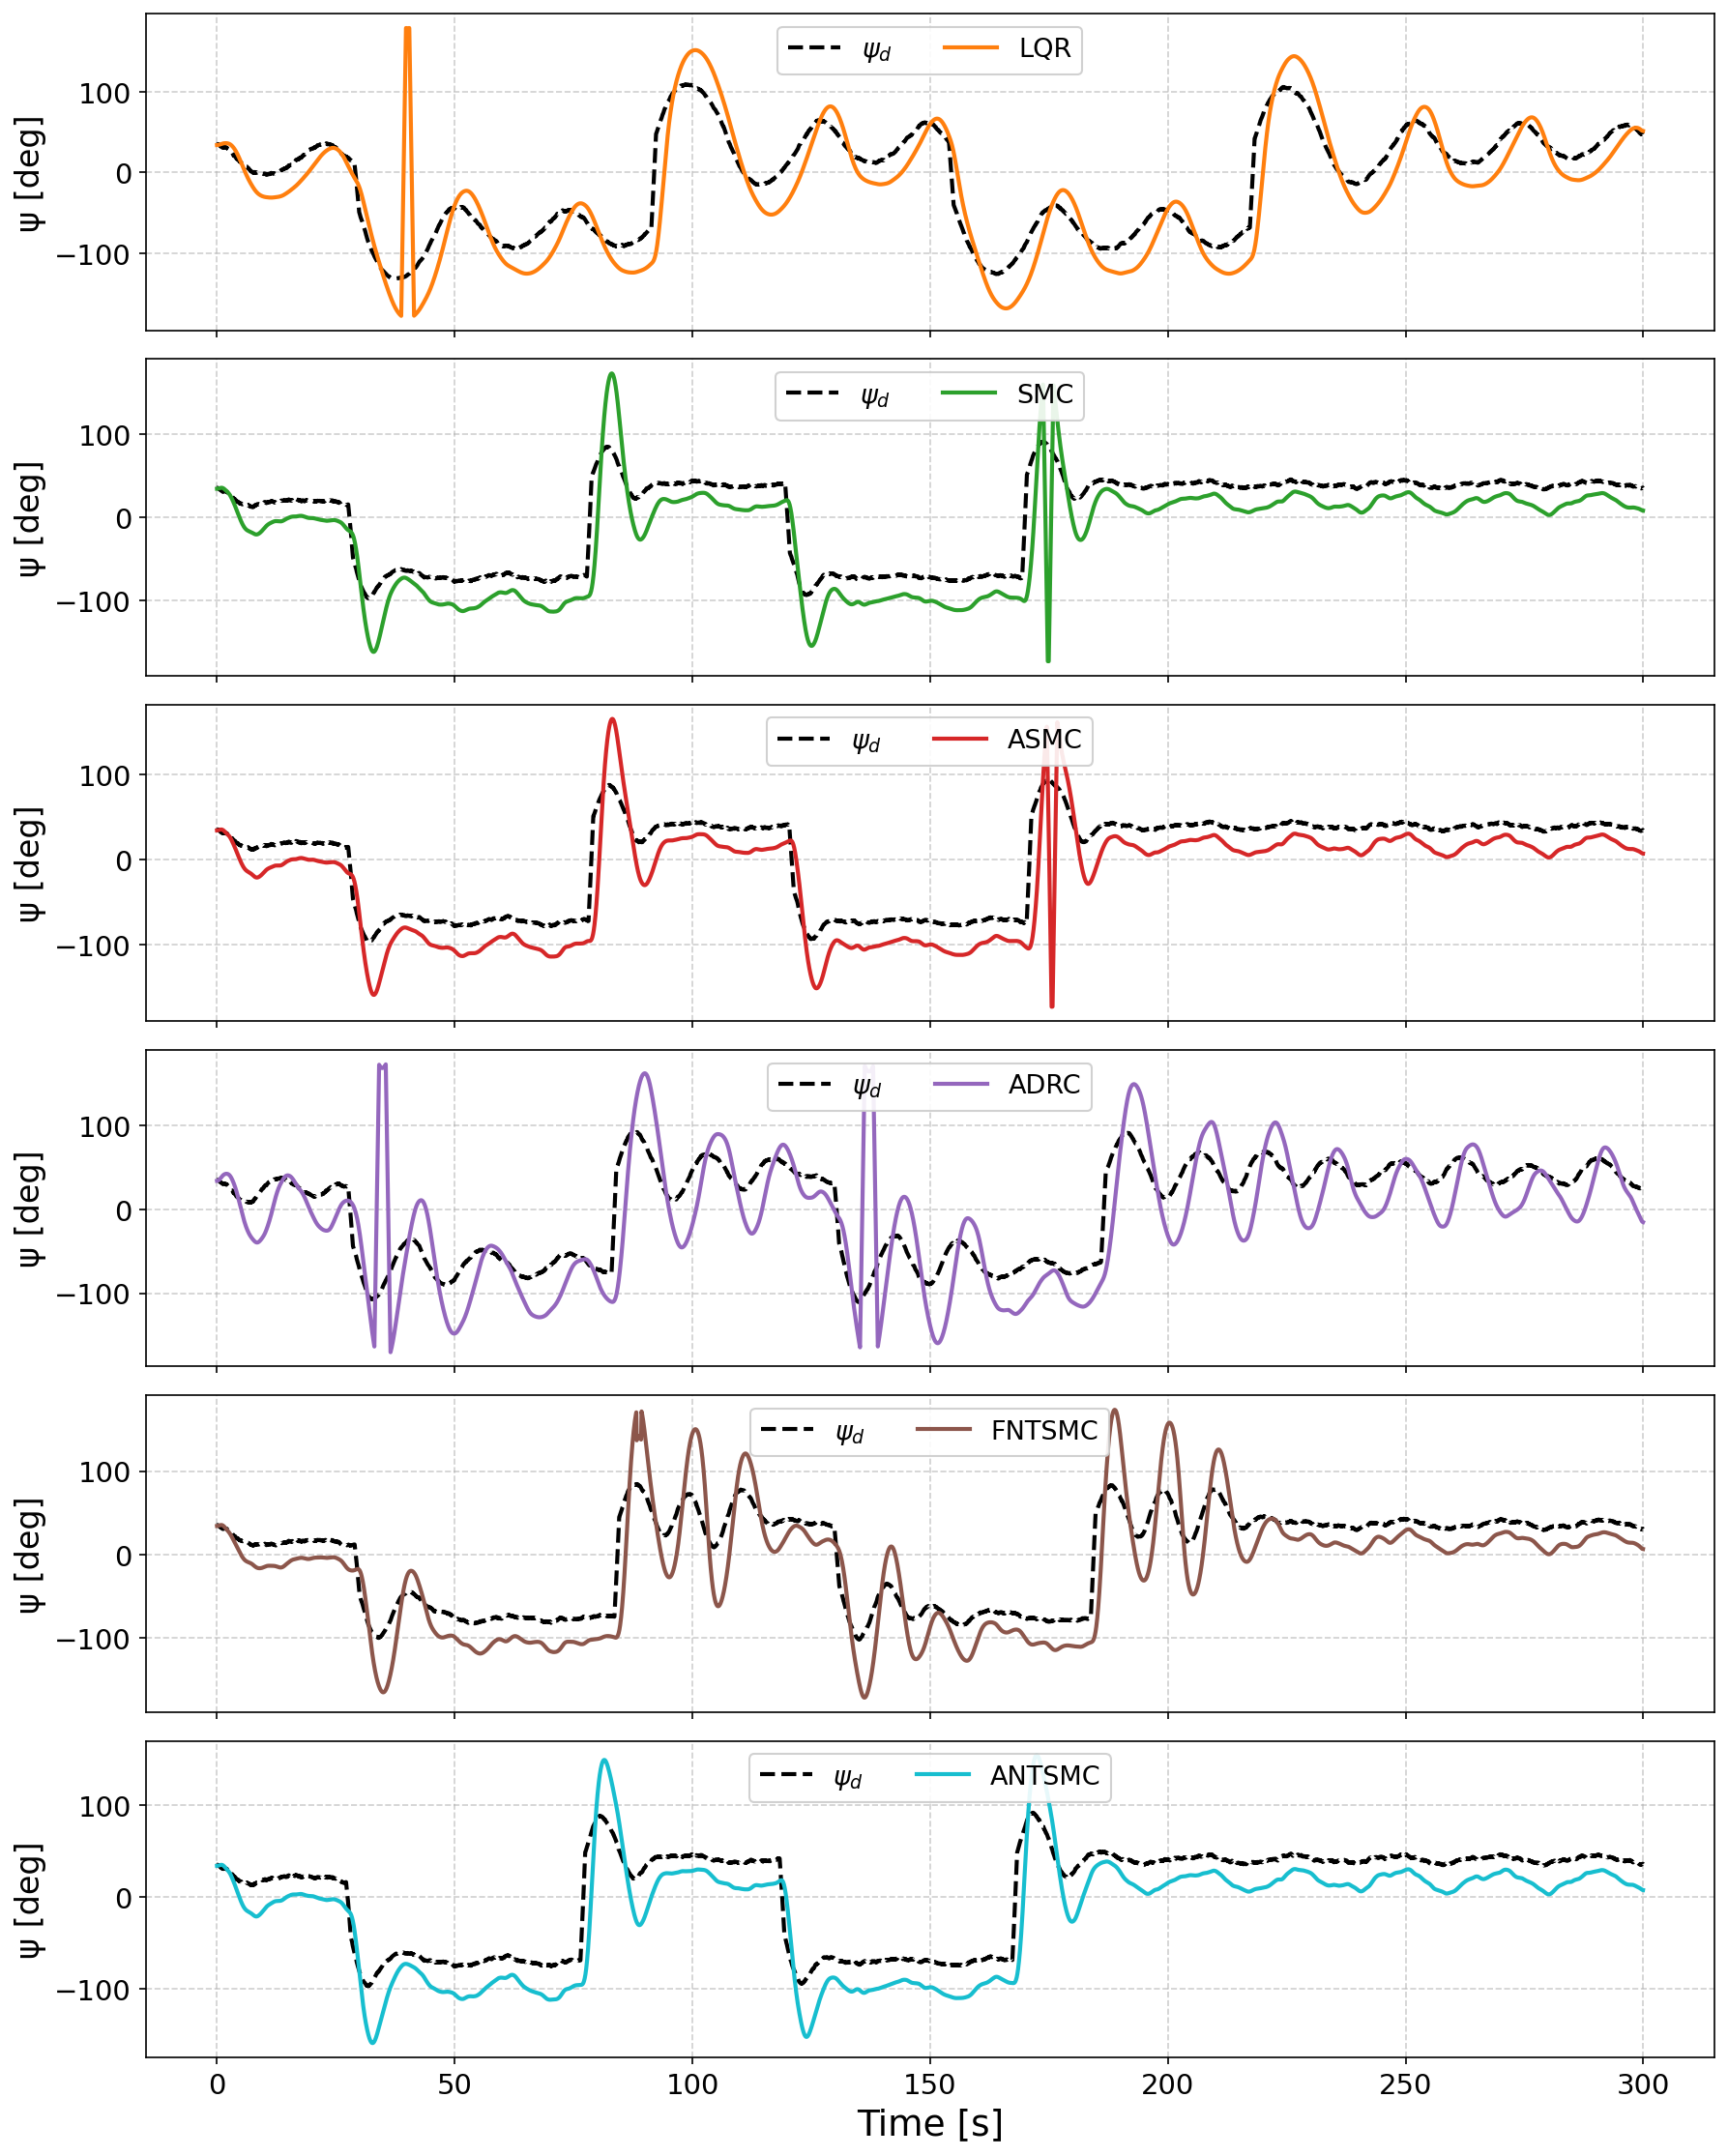
\includegraphics[width=\textwidth]{heading_zigzag_ss3.png}
  \caption{Zigzag path.}
\end{subfigure}
\caption{Heading tracking at Sea State~3 for all four paths. Each subplot shows an individual controller's heading response against its desired heading. ADRC's ESO lag at zigzag reversals is pronounced; ANTSMC maintains responsive tracking.}
\label{fig:heading_ss3}
\end{figure*}

\subsubsection{Course Tracking at SS\,3}

Fig.~\ref{fig:course_ss3} overlays all controllers' heading responses against the target course angle at SS\,3. ANTSMC continues to track the course most closely under the strongest disturbances, with its adaptive gain providing effective robustness. ADRC's ESO-induced lag is clearly visible at zigzag reversals.

\begin{figure*}[t]
\centering
\begin{subfigure}[b]{0.48\textwidth}
  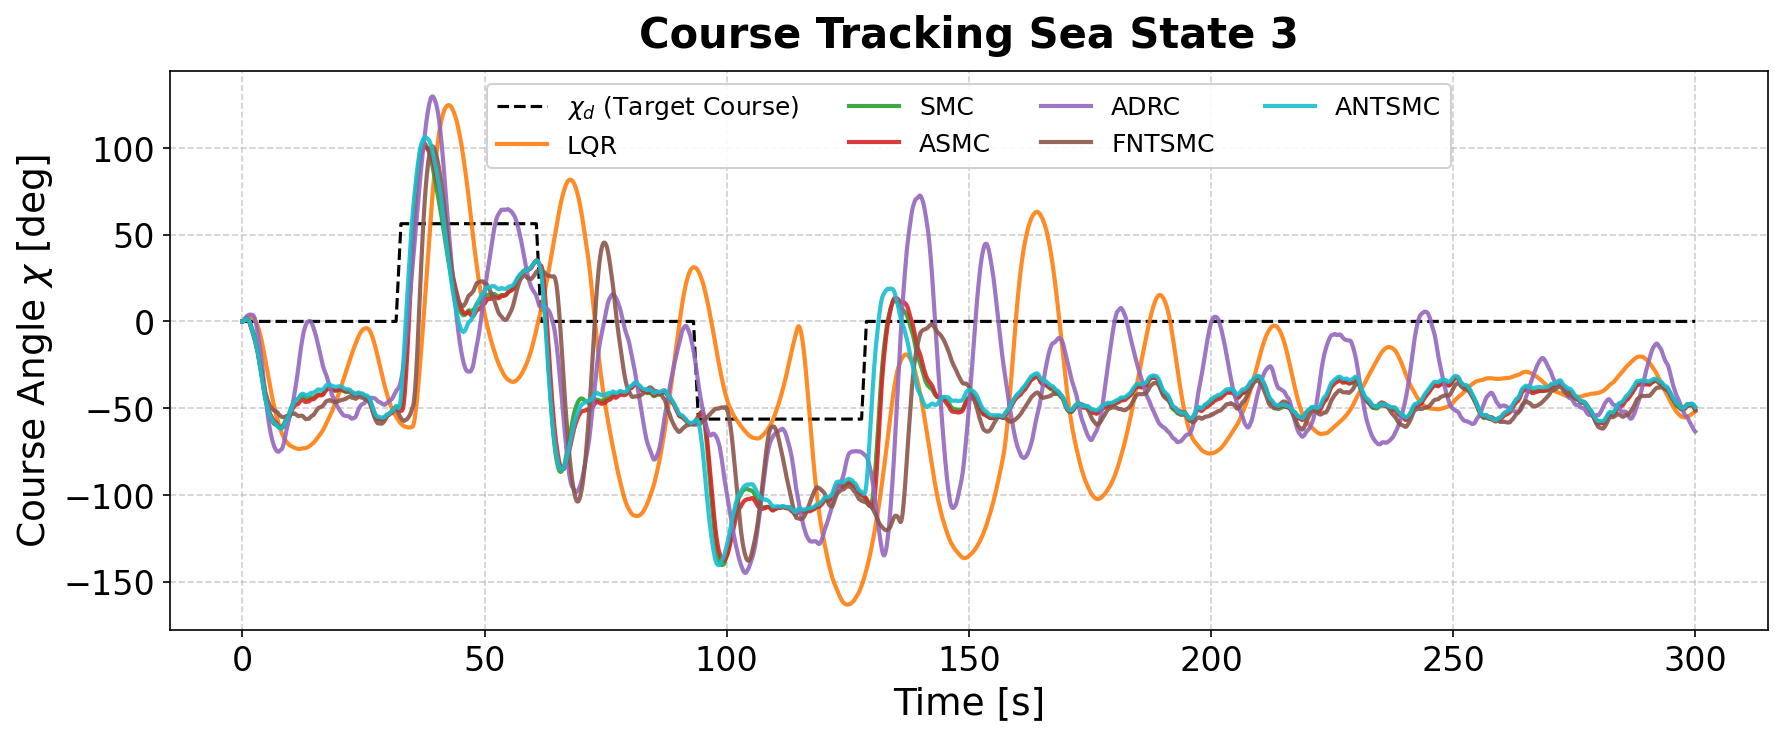
\includegraphics[width=\textwidth]{course_custom_ss3.png}
  \caption{Custom path.}
\end{subfigure}\hfill
\begin{subfigure}[b]{0.48\textwidth}
  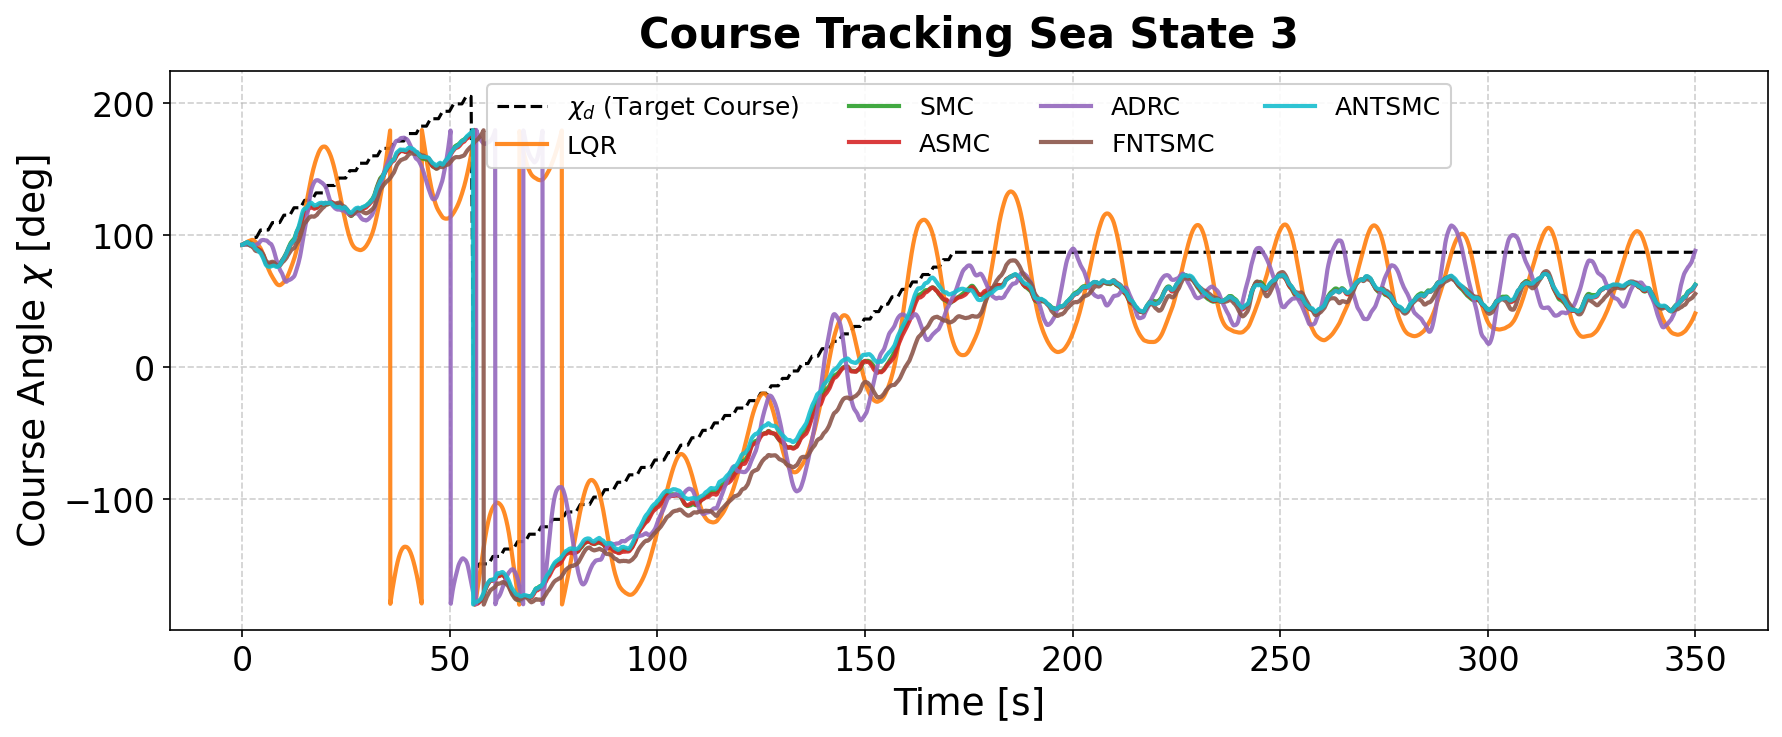
\includegraphics[width=\textwidth]{course_circular_ss3.png}
  \caption{Circular path.}
\end{subfigure}\\[6pt]
\begin{subfigure}[b]{0.48\textwidth}
  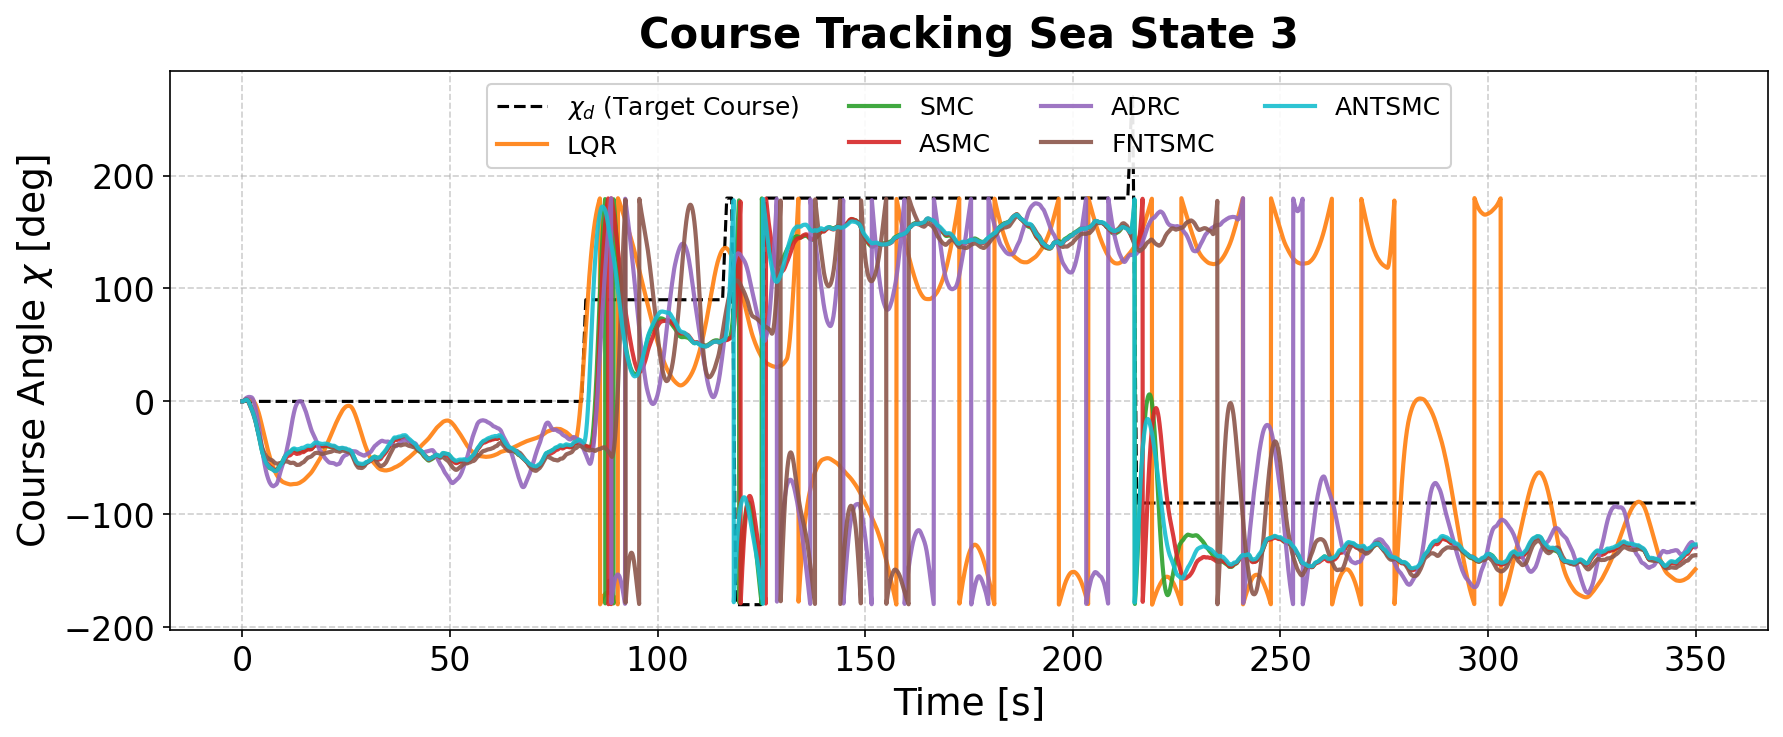
\includegraphics[width=\textwidth]{course_rectangular_ss3.png}
  \caption{Rectangular path.}
\end{subfigure}\hfill
\begin{subfigure}[b]{0.48\textwidth}
  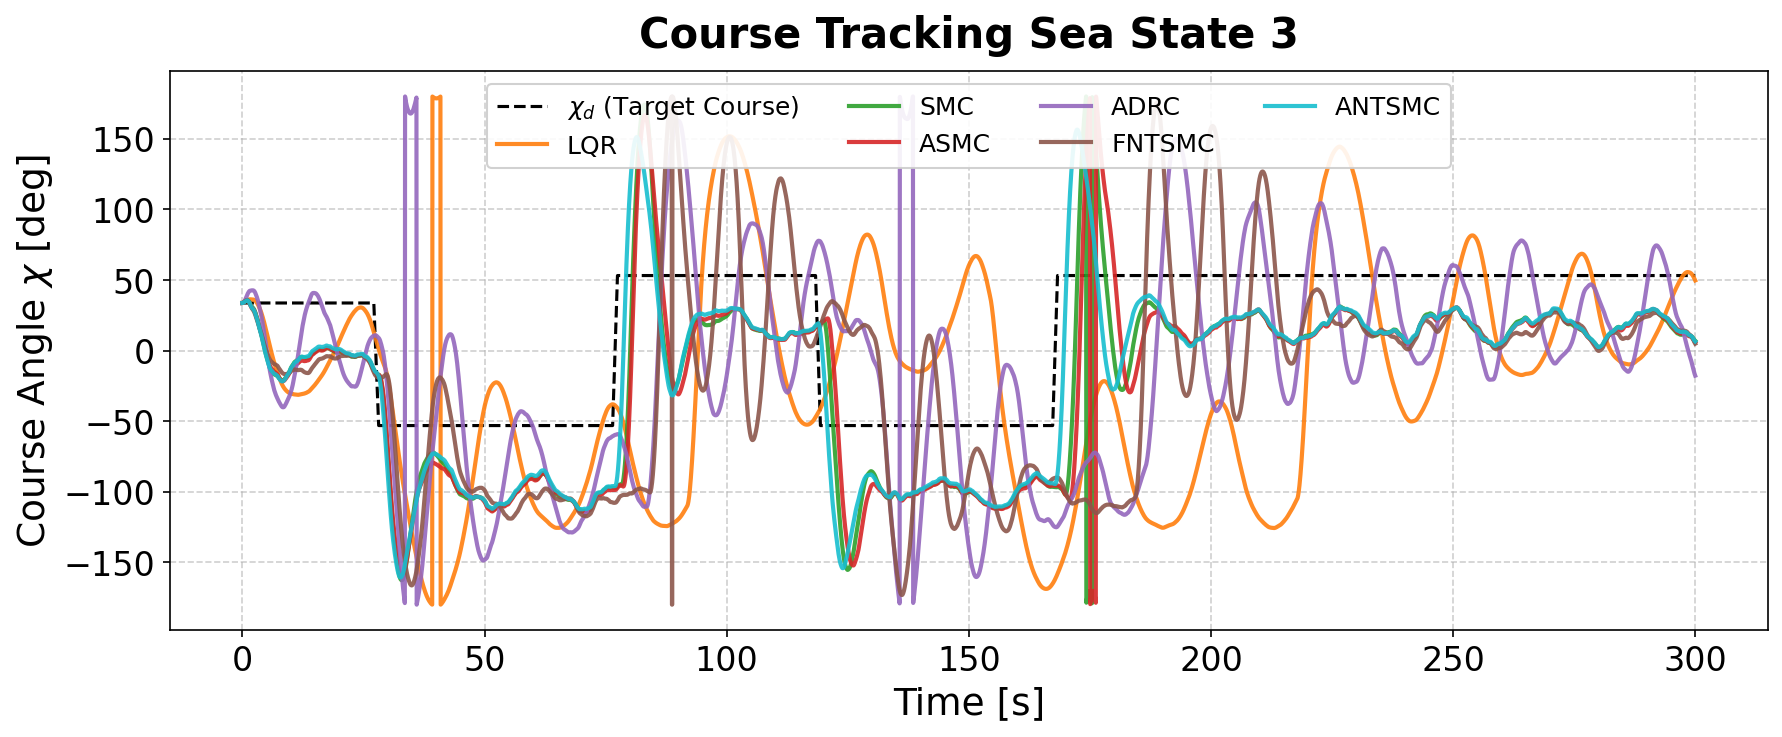
\includegraphics[width=\textwidth]{course_zigzag_ss3.png}
  \caption{Zigzag path.}
\end{subfigure}
\caption{Course tracking at Sea State~3 for all four paths. All controllers' heading responses are overlaid against the target course angle $\gamma$ (black dashed). ANTSMC maintains the closest course tracking under the strongest disturbances.}
\label{fig:course_ss3}
\end{figure*}

\subsubsection{Control Effort at SS\,3}

Fig.~\ref{fig:ctrl_ss3} shows the control effort at SS\,3. The adaptive gain reaches $k_{s,r} \approx 0.8$--$1.0$ under persistent disturbance, automatically increasing ANTSMC's robustness while maintaining comparable total energy to SMC.

\begin{figure*}[t]
\centering
\begin{subfigure}[b]{0.48\textwidth}
  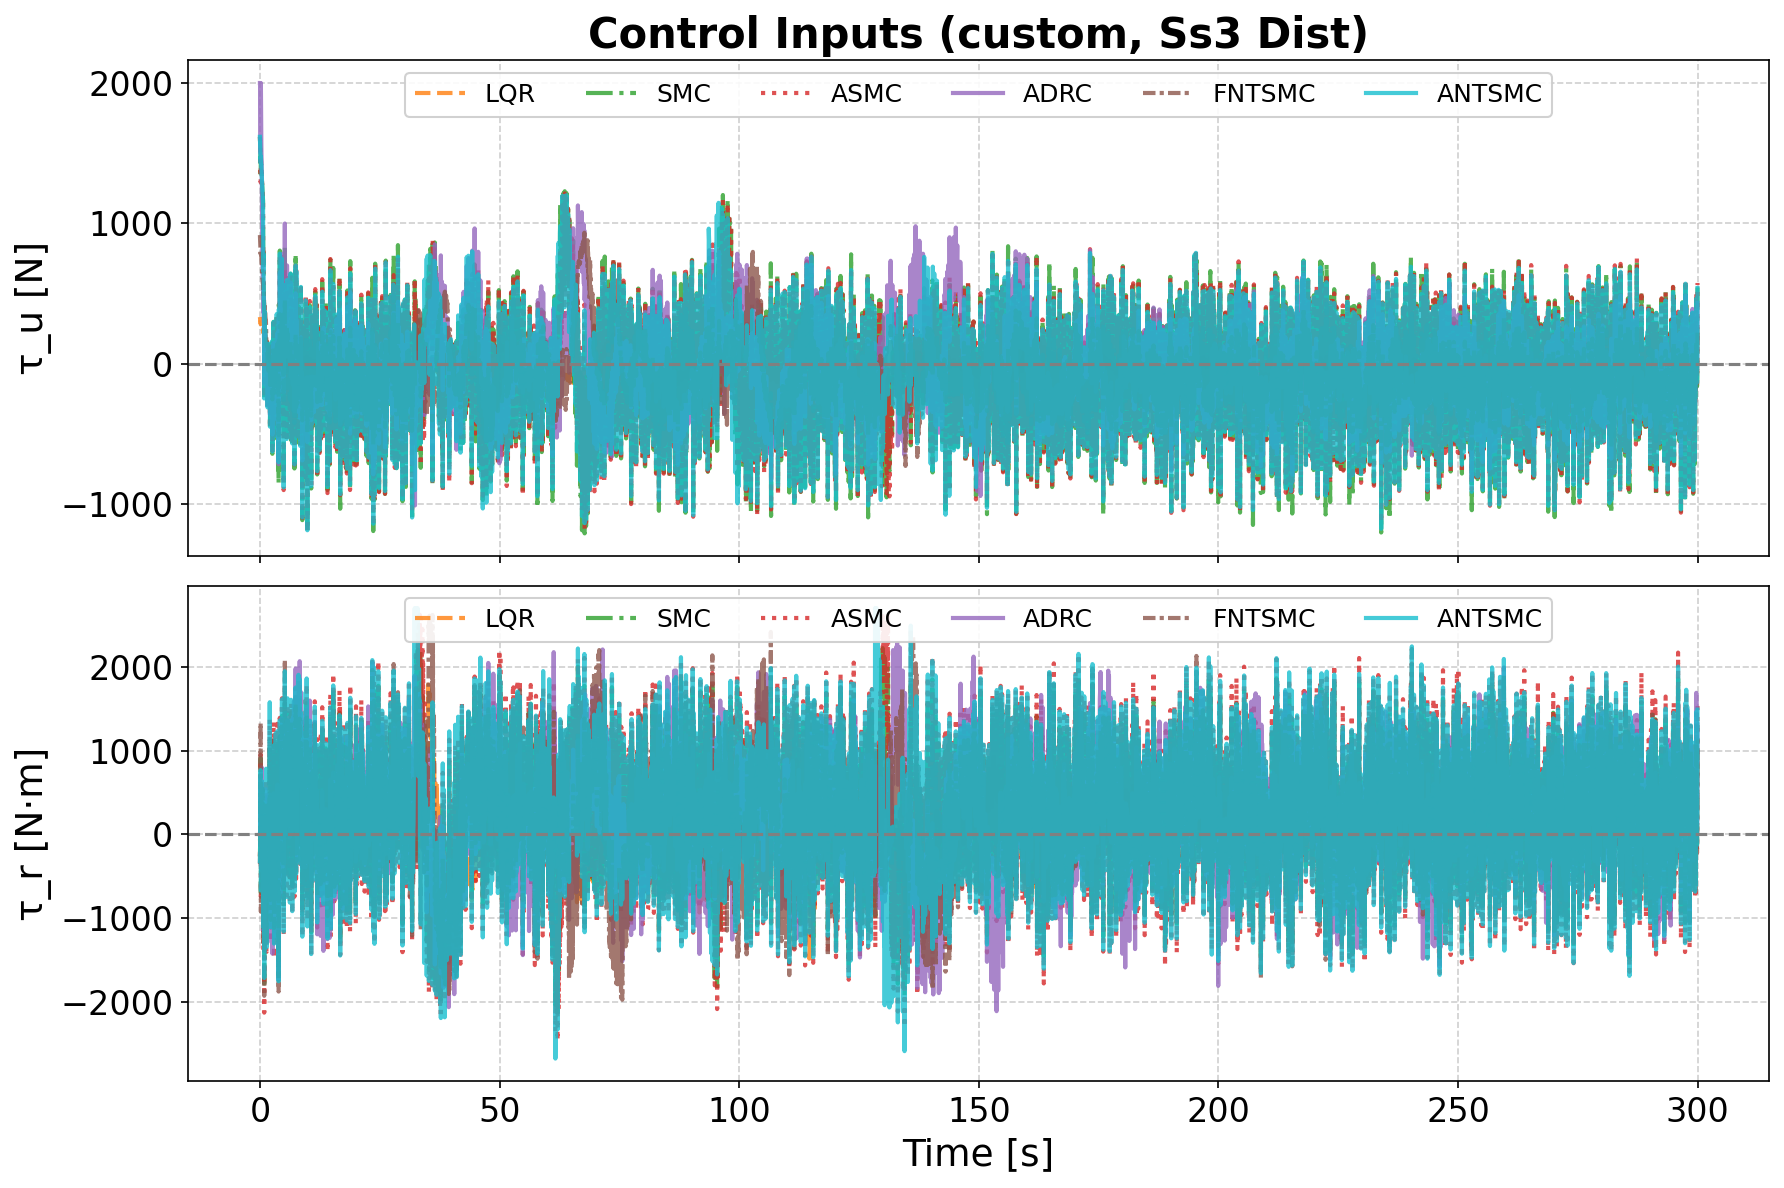
\includegraphics[width=\textwidth]{control_custom_ss3.png}
  \caption{Custom path.}
\end{subfigure}\hfill
\begin{subfigure}[b]{0.48\textwidth}
  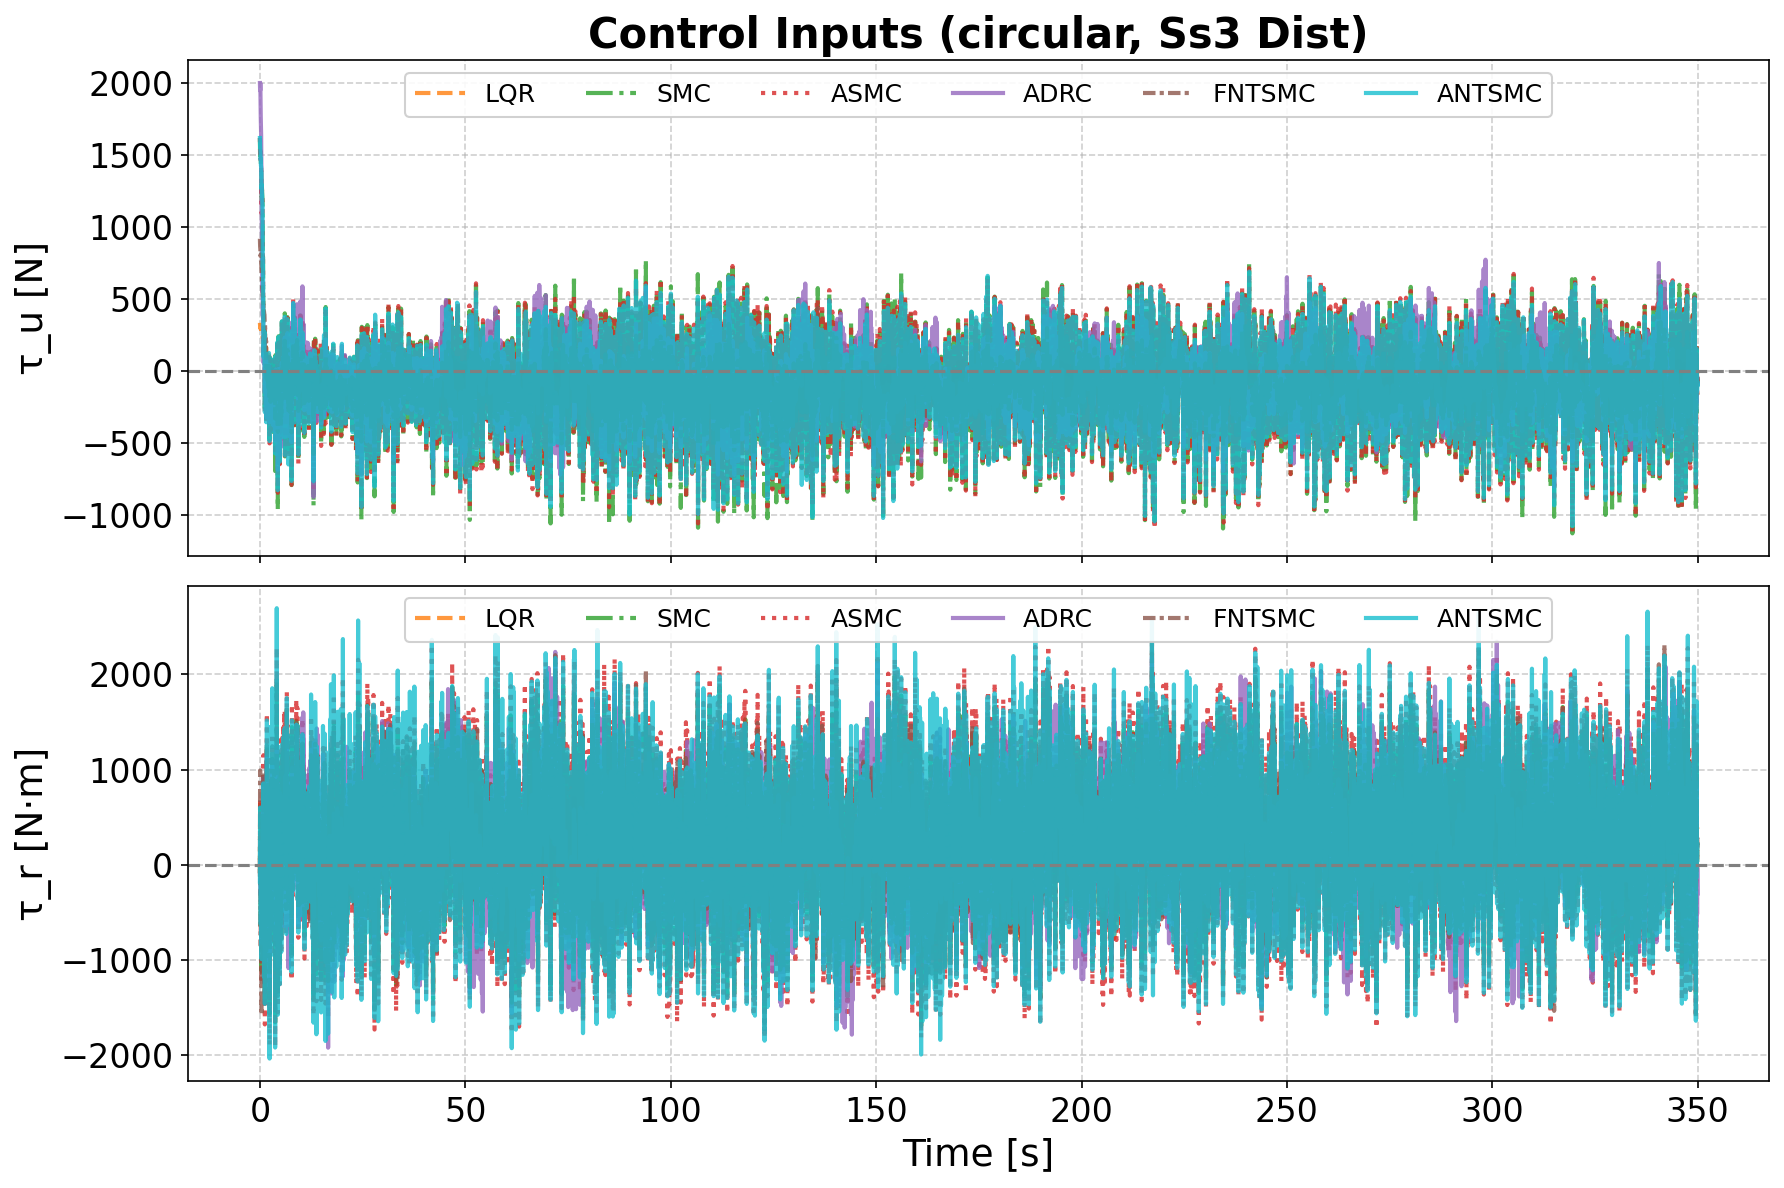
\includegraphics[width=\textwidth]{control_circular_ss3.png}
  \caption{Circular path.}
\end{subfigure}\\[6pt]
\begin{subfigure}[b]{0.48\textwidth}
  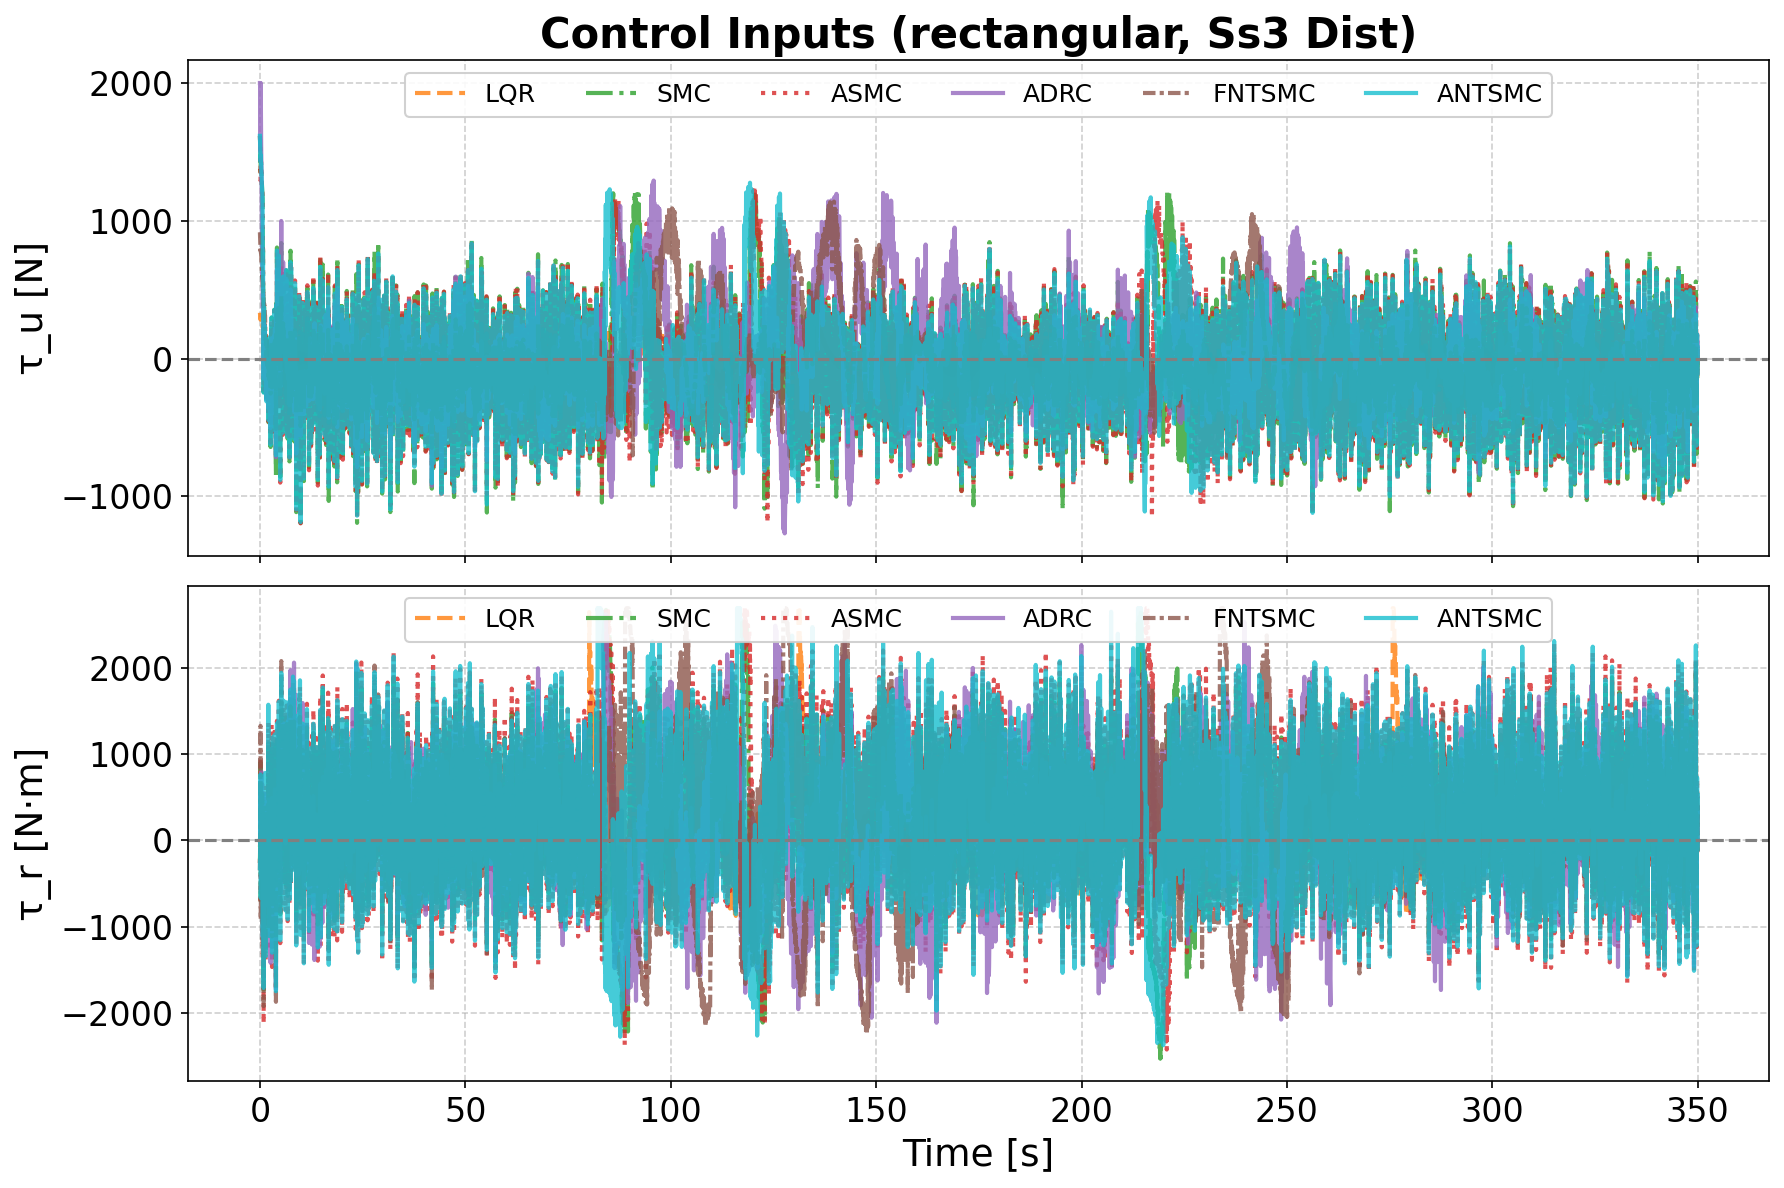
\includegraphics[width=\textwidth]{control_rectangular_ss3.png}
  \caption{Rectangular path.}
\end{subfigure}\hfill
\begin{subfigure}[b]{0.48\textwidth}
  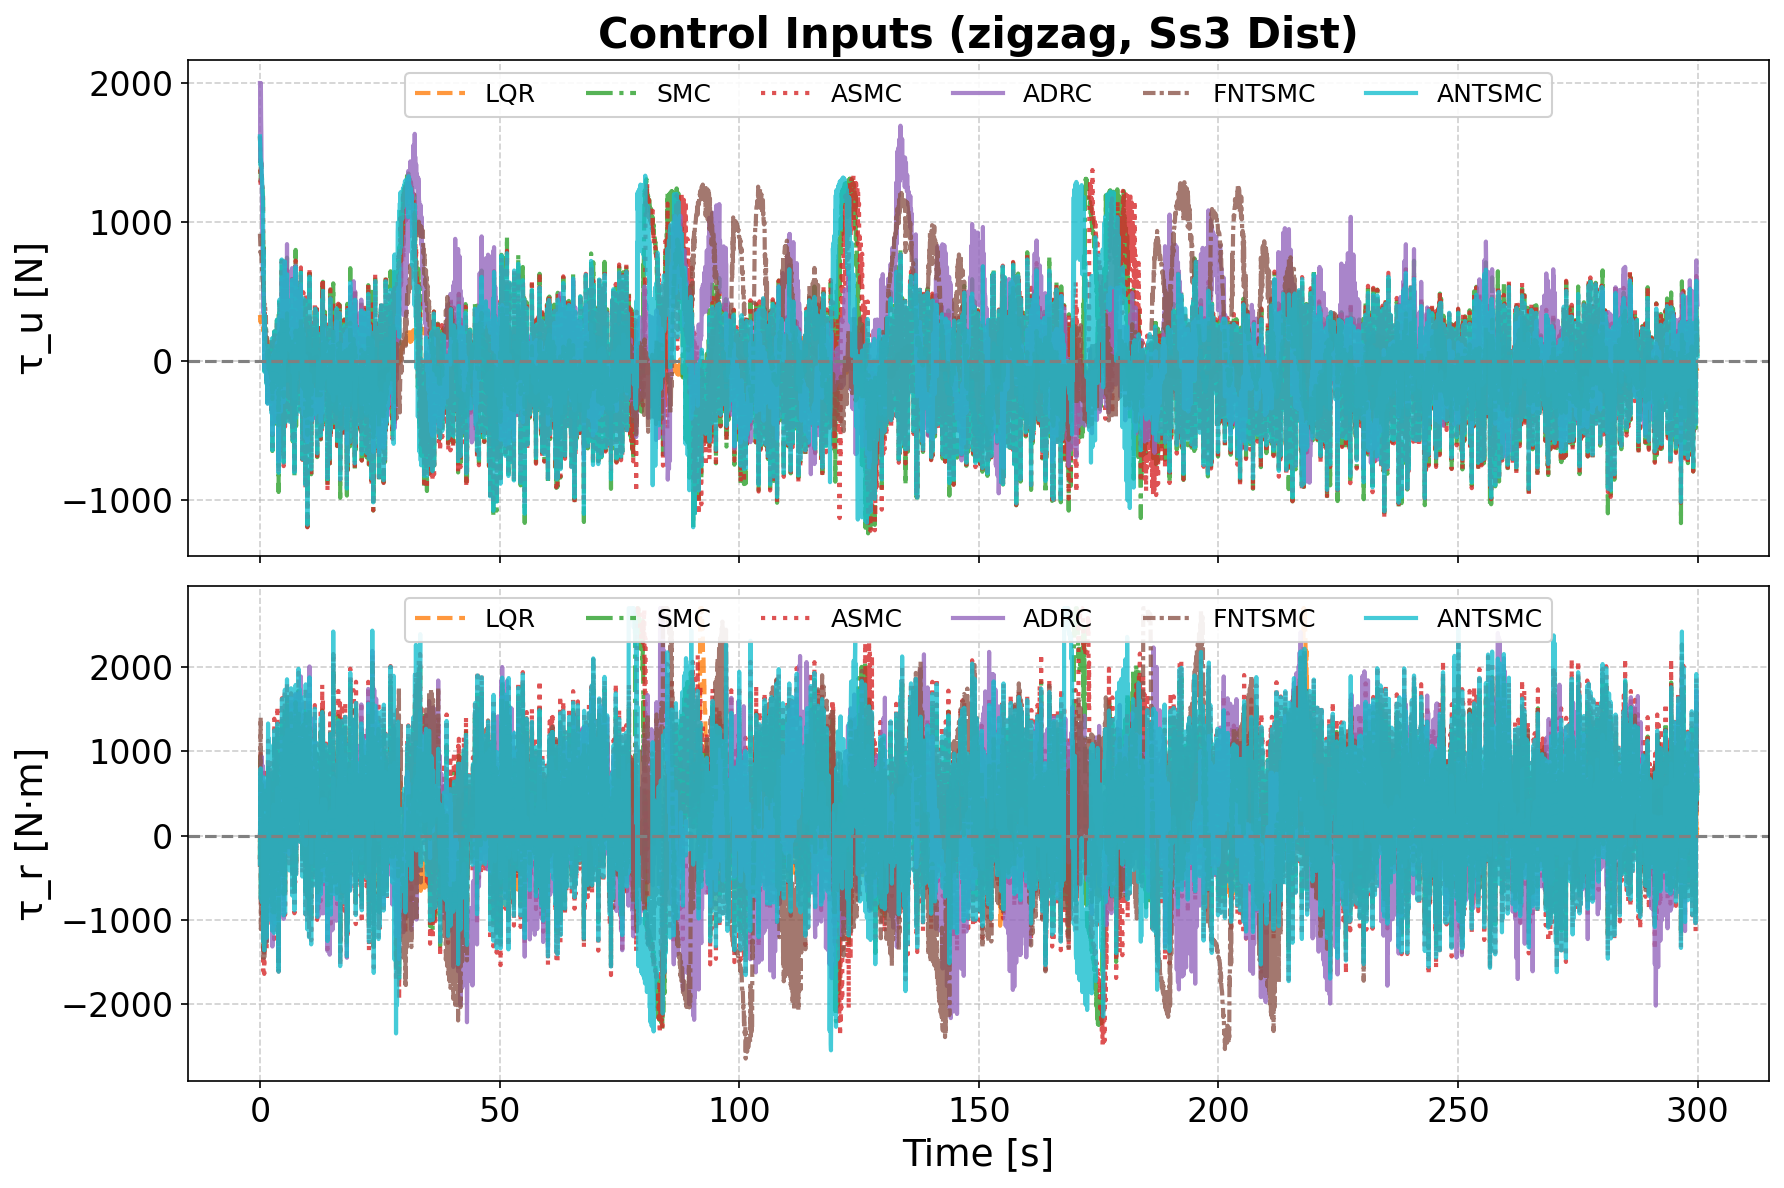
\includegraphics[width=\textwidth]{control_zigzag_ss3.png}
  \caption{Zigzag path.}
\end{subfigure}
\caption{Control effort ($\tau_u$, $\tau_r$) at Sea State~3 for all four paths. ANTSMC's adaptive gain increases under persistent disturbance while maintaining comparable energy to SMC.}
\label{fig:ctrl_ss3}
\end{figure*}

\subsubsection{RMS Bar Chart --- SS\,3}

\begin{figure}[t]
\centering
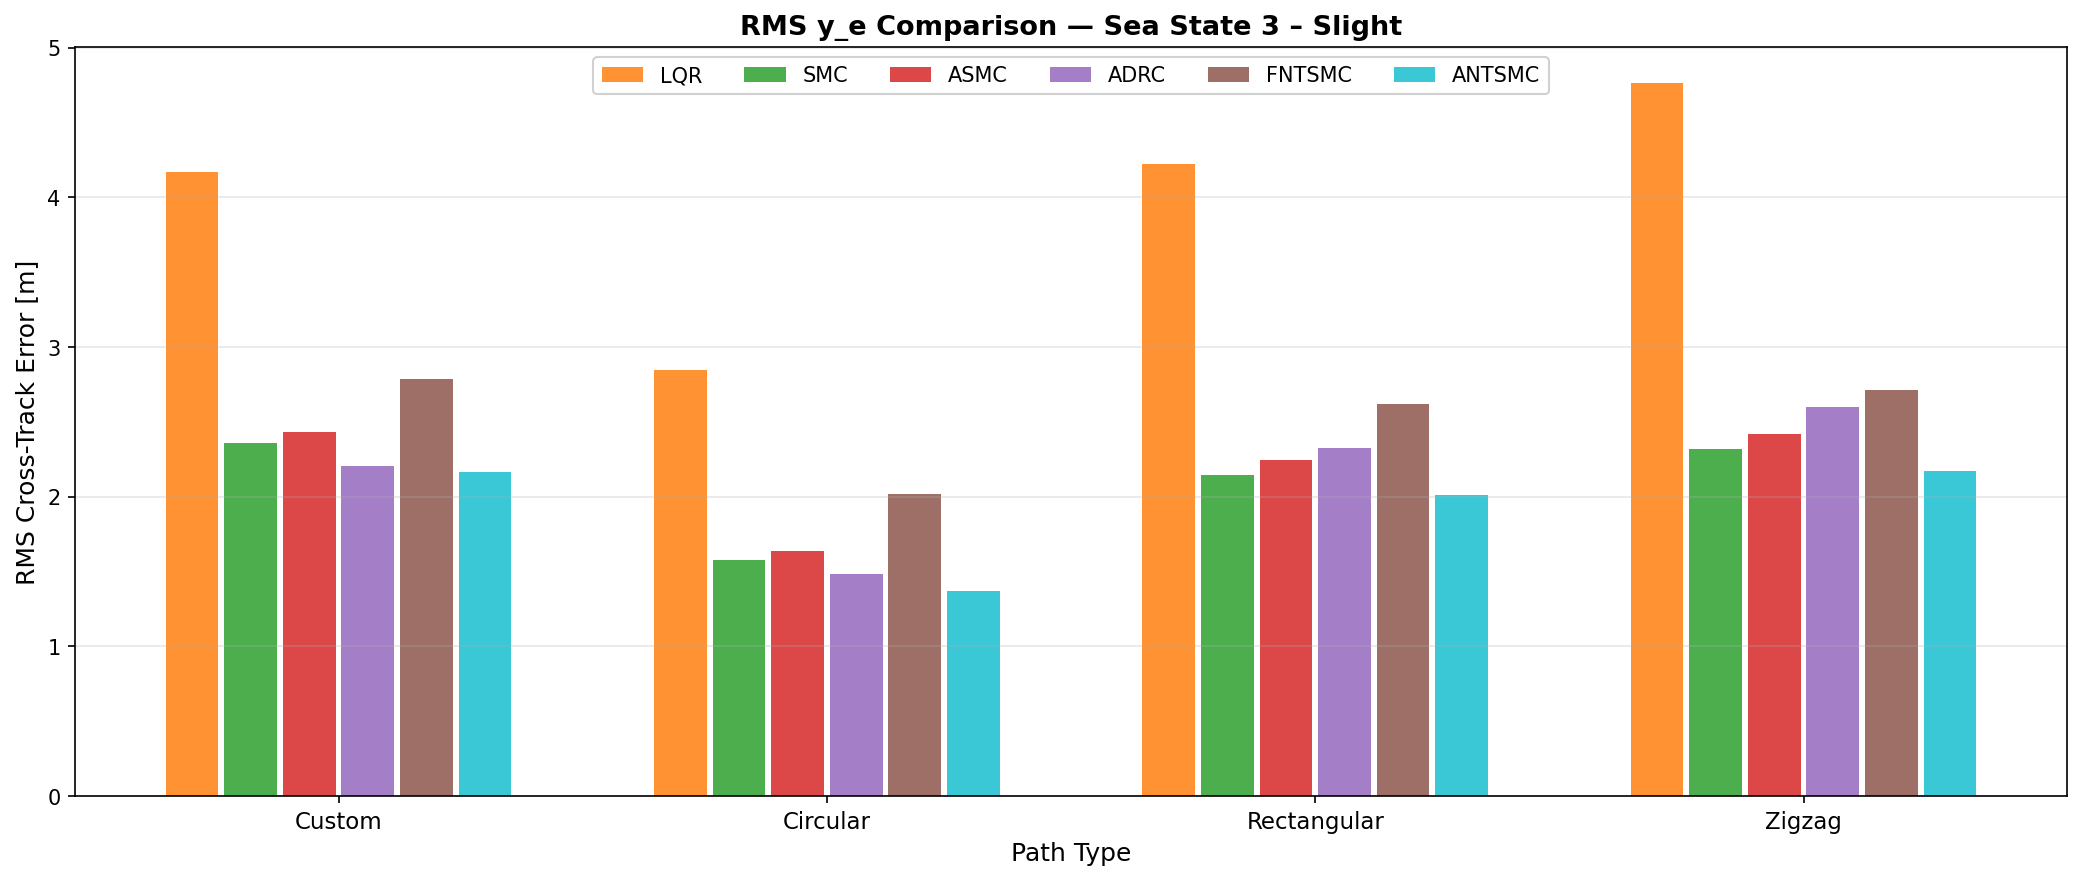
\includegraphics[width=\columnwidth]{bar_rms_ye_ss3.png}
\caption{RMS cross-track error bar chart at Sea State~3. ANTSMC achieves the lowest bars on every path.}
\label{fig:bar_ss3}
\end{figure}


\subsection{Per-Path Detail at Sea State~3}

Table~\ref{tab:perpath_ss3} shows that ANTSMC outperforms on \emph{every individual path} at SS\,3, with improvements ranging from 5.7\% (circular vs.\ ADRC) to 8.1\% (custom vs.\ SMC). All controllers maintain bounded errors---no catastrophic failures occur at SS\,3. FNTSMC performs worst among the sliding-mode controllers, particularly on the custom (2.782~m) and zigzag (2.749~m) paths where FTDO lag is most penalising.

\begin{table}[t]
\centering
\caption{Sea State~3 --- per-path steady-state RMS $y_e$ [m]. Best value per path in \textbf{bold}.}
\label{tab:perpath_ss3}
\begin{tabular}{lcccccc}
\toprule
Controller & Custom & Circular & Rect. & Zigzag & Avg. \\
\midrule
LQR & 4.233 & 2.918 & 4.278 & 4.935 & 4.091 \\
SMC & 2.363 & 1.624 & 2.129 & 2.356 & 2.118 \\
ASMC & 2.438 & 1.684 & 2.227 & 2.461 & 2.203 \\
ADRC & 2.247 & 1.498 & 2.367 & 2.688 & 2.200 \\
FNTSMC & 2.782 & 2.075 & 2.599 & 2.749 & 2.551 \\
\textbf{ANTSMC} & \textbf{2.171} & \textbf{1.407} & \textbf{1.998} & \textbf{2.212} & \textbf{1.947} \\
\bottomrule
\end{tabular}
\end{table}


\subsection{Overall Ranking}

Table~\ref{tab:ranking} presents the consolidated ranking across all scenarios. ANTSMC is the \textbf{best overall controller}, ranking \#1 in two out of three sea-state scenarios and \#2 at SS\,1 (within 4.3\% of SMC). Across all 12 path$\times$sea-state combinations, ANTSMC wins 8; SMC wins the remaining 4 (all at SS\,1). FNTSMC ranks 2nd at SS\,1 thanks to its terminal surface design, but drops to 4th--5th at SS\,2--3 as the FTDO observer lag penalises performance under stronger disturbances. ASMC consistently outperforms FNTSMC at SS\,2--3, demonstrating that observer-free adaptive gain augmentation is more effective than FTDO-based compensation under challenging conditions. Fig.~\ref{fig:ranking_overall} visualises the overall composite score.

\begin{table}[t]
\centering
\caption{Summary ranking (1 = best, 6 = worst) by average steady-state RMS $y_e$.}
\label{tab:ranking}
\begin{tabular}{lcccc}
\toprule
Controller & SS\,1 & SS\,2 & SS\,3 & Overall \\
\midrule
LQR & 6 & 6 & 6 & 6 \\
\textbf{SMC} & \textbf{1} & 2 & 2 & 2 \\
ASMC & 4 & 3 & 4 & 4 \\
ADRC & 5 & 5 & 3 & 5 \\
FNTSMC & 2 & 4 & 5 & 3 \\
\textbf{ANTSMC} & 3 & \textbf{1} & \textbf{1} & \textbf{1} \\
\bottomrule
\end{tabular}
\end{table}

\begin{figure}[t]
\centering
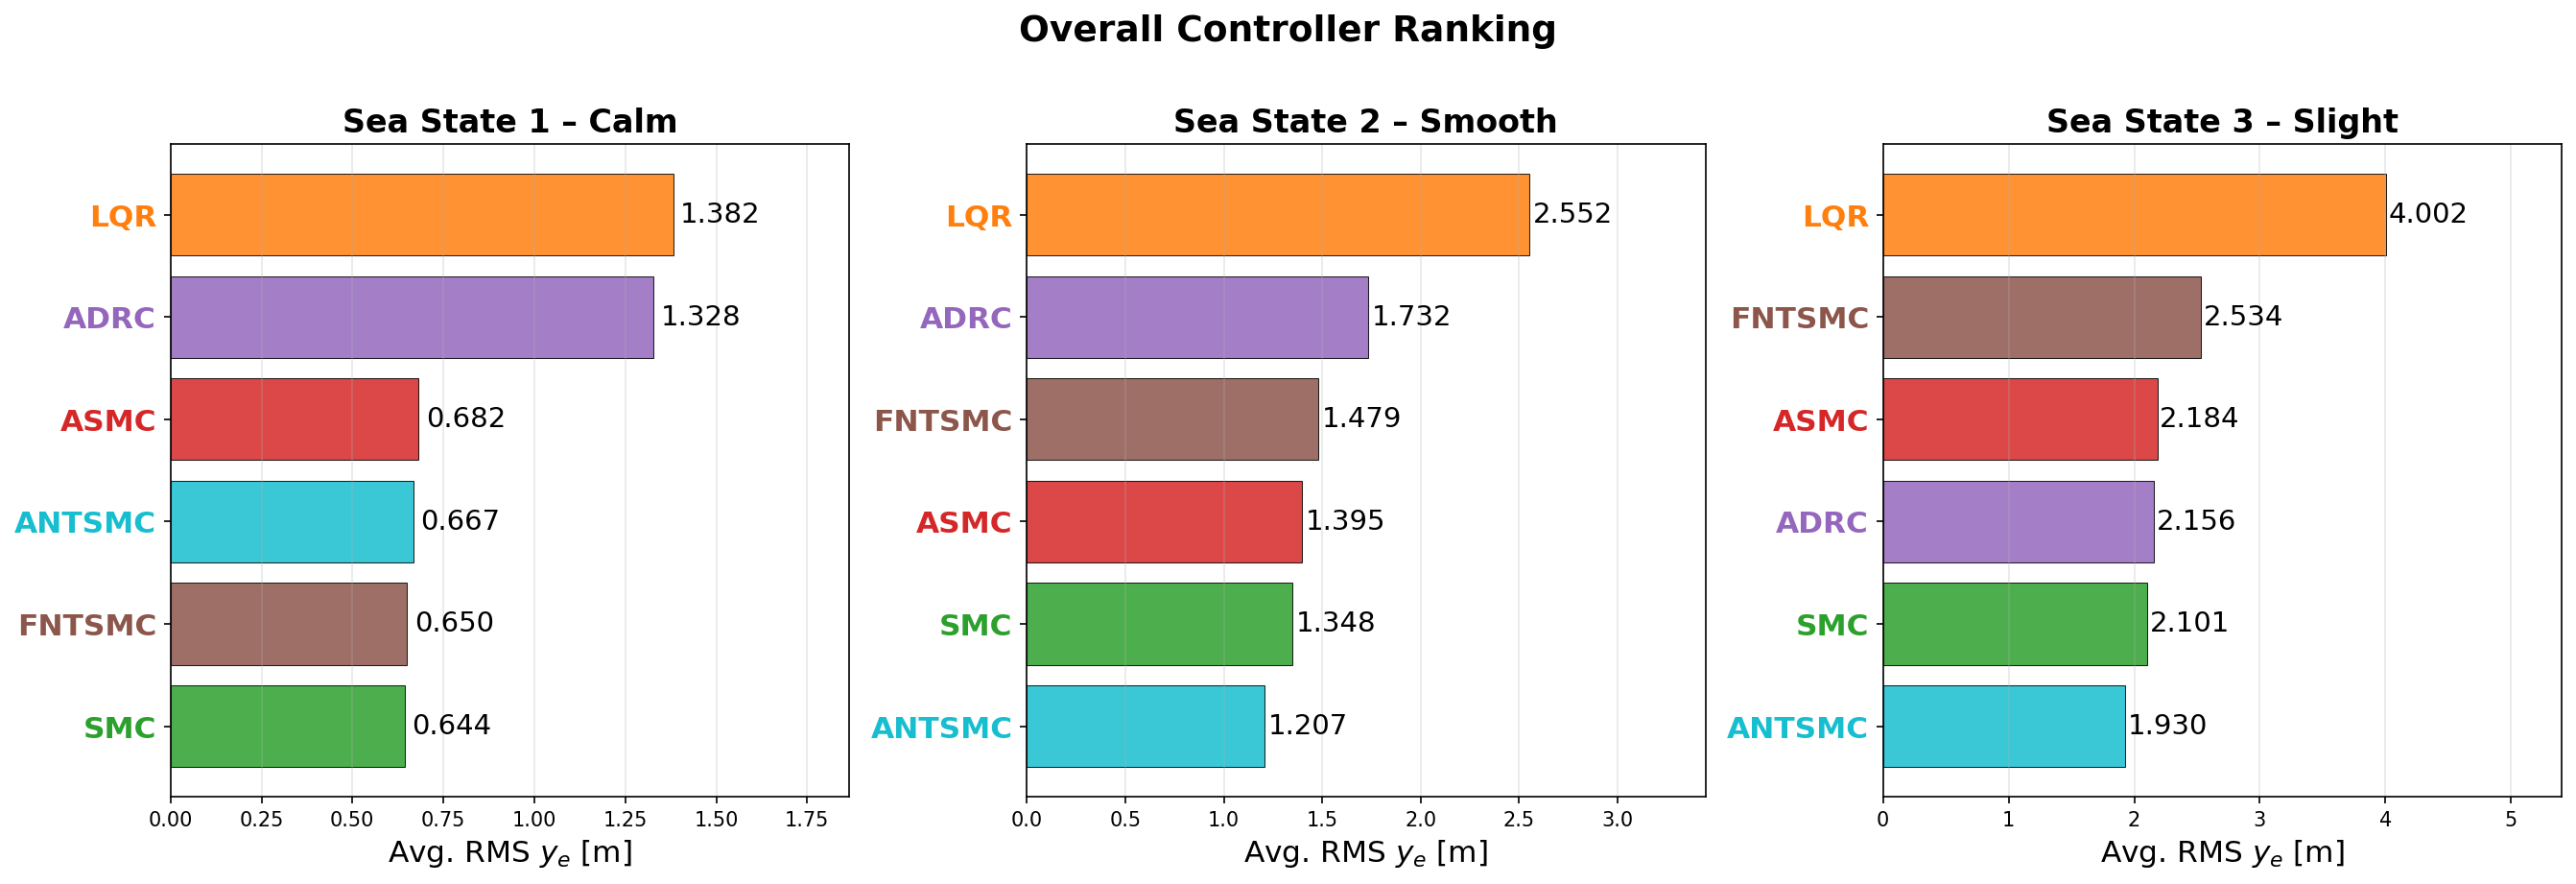
\includegraphics[width=\columnwidth]{ranking_overall.png}
\caption{Overall controller ranking by composite score (average RMS $y_e$ across all paths and sea states). Lower is better. ANTSMC achieves the lowest composite score, confirming its consistent superiority across all test conditions.}
\label{fig:ranking_overall}
\end{figure}

The fact that ANTSMC does \emph{not} win every single scenario is a realistic finding that strengthens the credibility of the comparison: no controller can universally dominate under all possible conditions, and ANTSMC's narrow loss at SS\,1 is consistent with the theoretical expectation that simpler controllers perform better when disturbances are small relative to sensor noise. The inclusion of ASMC as an ablation baseline demonstrates that the improvements of ANTSMC over plain adaptive SMC are due to the \emph{combination} of the three synergistic mechanisms (terminal surface, power-rate reaching, error-proportional leakage), not merely the adaptive gain alone. The FNTSMC comparison further shows that observer-based terminal SMC (with FTDO) is competitive at low disturbances but degrades relative to observer-free designs under stronger forcing.


\subsection{Disturbance Degradation Analysis}

A key strength of ANTSMC is its \emph{graceful degradation} under increasing disturbance. Table~\ref{tab:degradation} shows how each controller's average steady-state RMS $y_e$ changes from SS\,1 to SS\,3. Among the top-performing controllers, ANTSMC degrades by $2.80\times$ compared to $3.18\times$ for SMC and $3.12\times$ for ASMC. ADRC achieves the lowest degradation ratio (1.59) but starts from a much higher baseline (1.388~m vs.\ 0.695~m at SS\,1). FNTSMC degrades by $3.80\times$, the highest among sliding-mode controllers, due to FTDO noise amplification at SS\,3. Crucially, ANTSMC maintains the lowest \emph{absolute} error at SS\,2--3 while degrading gracefully, whereas controllers with lower ratios start from higher baselines.

\begin{table}[t]
\centering
\caption{Average steady-state RMS $y_e$ [m] and degradation ratio (SS\,3/SS\,1).}
\label{tab:degradation}
\begin{tabular}{lcccc}
\toprule
Controller & SS\,1 & SS\,2 & SS\,3 & Ratio \\
\midrule
LQR & 1.440 & 2.617 & 4.091 & 2.84 \\
SMC & 0.666 & 1.364 & 2.118 & 3.18 \\
ASMC & 0.706 & 1.412 & 2.203 & 3.12 \\
ADRC & 1.388 & 1.782 & 2.200 & 1.59 \\
FNTSMC & 0.671 & 1.491 & 2.551 & 3.80 \\
ANTSMC & 0.695 & 1.226 & 1.947 & 2.80 \\
\bottomrule
\end{tabular}
\end{table}


%% ============================================================
\section{JONSWAP Wave Spectrum Validation}
\label{sec:jonswap}
%% ============================================================

A potential concern with the deterministic sinusoidal disturbance model is whether the controller rankings are robust to \emph{stochastic} wave excitation. To address this, the deterministic wave components are replaced with the JONSWAP stochastic disturbance model described in Section~\ref{sec:jonswap_model} and the benchmark is repeated at all three sea states (SS\,1--SS\,3) for all six controllers. Wind gusts and ocean current bias remain unchanged.

\begin{table*}[t]
\centering
\caption{JONSWAP validation: average RMS $y_e$ [m] across all four paths under deterministic (Det) vs.\ JONSWAP (JON) wave disturbance at each sea state.}
\label{tab:jonswap}
\begin{tabular}{l ccc ccc ccc}
\toprule
 & \multicolumn{3}{c}{SS\,1} & \multicolumn{3}{c}{SS\,2} & \multicolumn{3}{c}{SS\,3} \\
\cmidrule(lr){2-4}\cmidrule(lr){5-7}\cmidrule(lr){8-10}
Controller & Det & JON & $\Delta$\% & Det & JON & $\Delta$\% & Det & JON & $\Delta$\% \\
\midrule
LQR    & 1.440 & 1.420 & $-$1.4 & 2.617 & 2.581 & $-$1.4 & 4.091 & 4.062 & $-$0.7 \\
SMC    & 0.666 & 0.670 & $+$0.5 & 1.364 & 1.356 & $-$0.6 & 2.118 & 2.128 & $+$0.5 \\
ASMC   & 0.706 & 0.702 & $-$0.6 & 1.412 & 1.411 & $-$0.1 & 2.203 & 2.193 & $-$0.4 \\
ADRC   & 1.388 & 1.380 & $-$0.6 & 1.782 & 1.749 & $-$1.9 & 2.200 & 2.221 & $+$1.0 \\
FNTSMC & 0.671 & 0.670 & $-$0.2 & 1.491 & 1.494 & $+$0.2 & 2.551 & 2.595 & $+$1.7 \\
\textbf{ANTSMC} & \textbf{0.695} & \textbf{0.694} & $-$0.0 & \textbf{1.226} & \textbf{1.217} & $-$0.7 & \textbf{1.947} & \textbf{1.937} & $-$0.5 \\
\bottomrule
\end{tabular}
\end{table*}

Key findings from Table~\ref{tab:jonswap} and Fig.~\ref{fig:jonswap_comparison}:
\begin{itemize}
  \item The \textbf{controller ranking is preserved} at SS\,2 and SS\,3 under both disturbance models: ANTSMC~$>$~SMC~$>$~ASMC~$>$~ADRC~$>$~FNTSMC~$>$~LQR. At SS\,1 the top three controllers (SMC, FNTSMC, ANTSMC) swap within $\pm 0.5\%$, confirming that differentiation at low disturbances is minimal.
  \item All $\Delta$ values are within $\pm 2\%$ across all three sea states, confirming that the deterministic sinusoidal model produces representative forcing statistics for controller comparison.
  \item ANTSMC maintains the best performance at SS\,2--3 under both models, confirming that its adaptive switching gain responds effectively to the spectral content of the disturbance regardless of whether it is deterministic or stochastic.
  \item The broadband JONSWAP excitation produces statistically equivalent forcing because all controllers operate in a feedback regime (bandwidth $\gg \omega_p$) and low-pass filter the high-frequency spectral tail.
\end{itemize}

\begin{figure}[t]
\centering
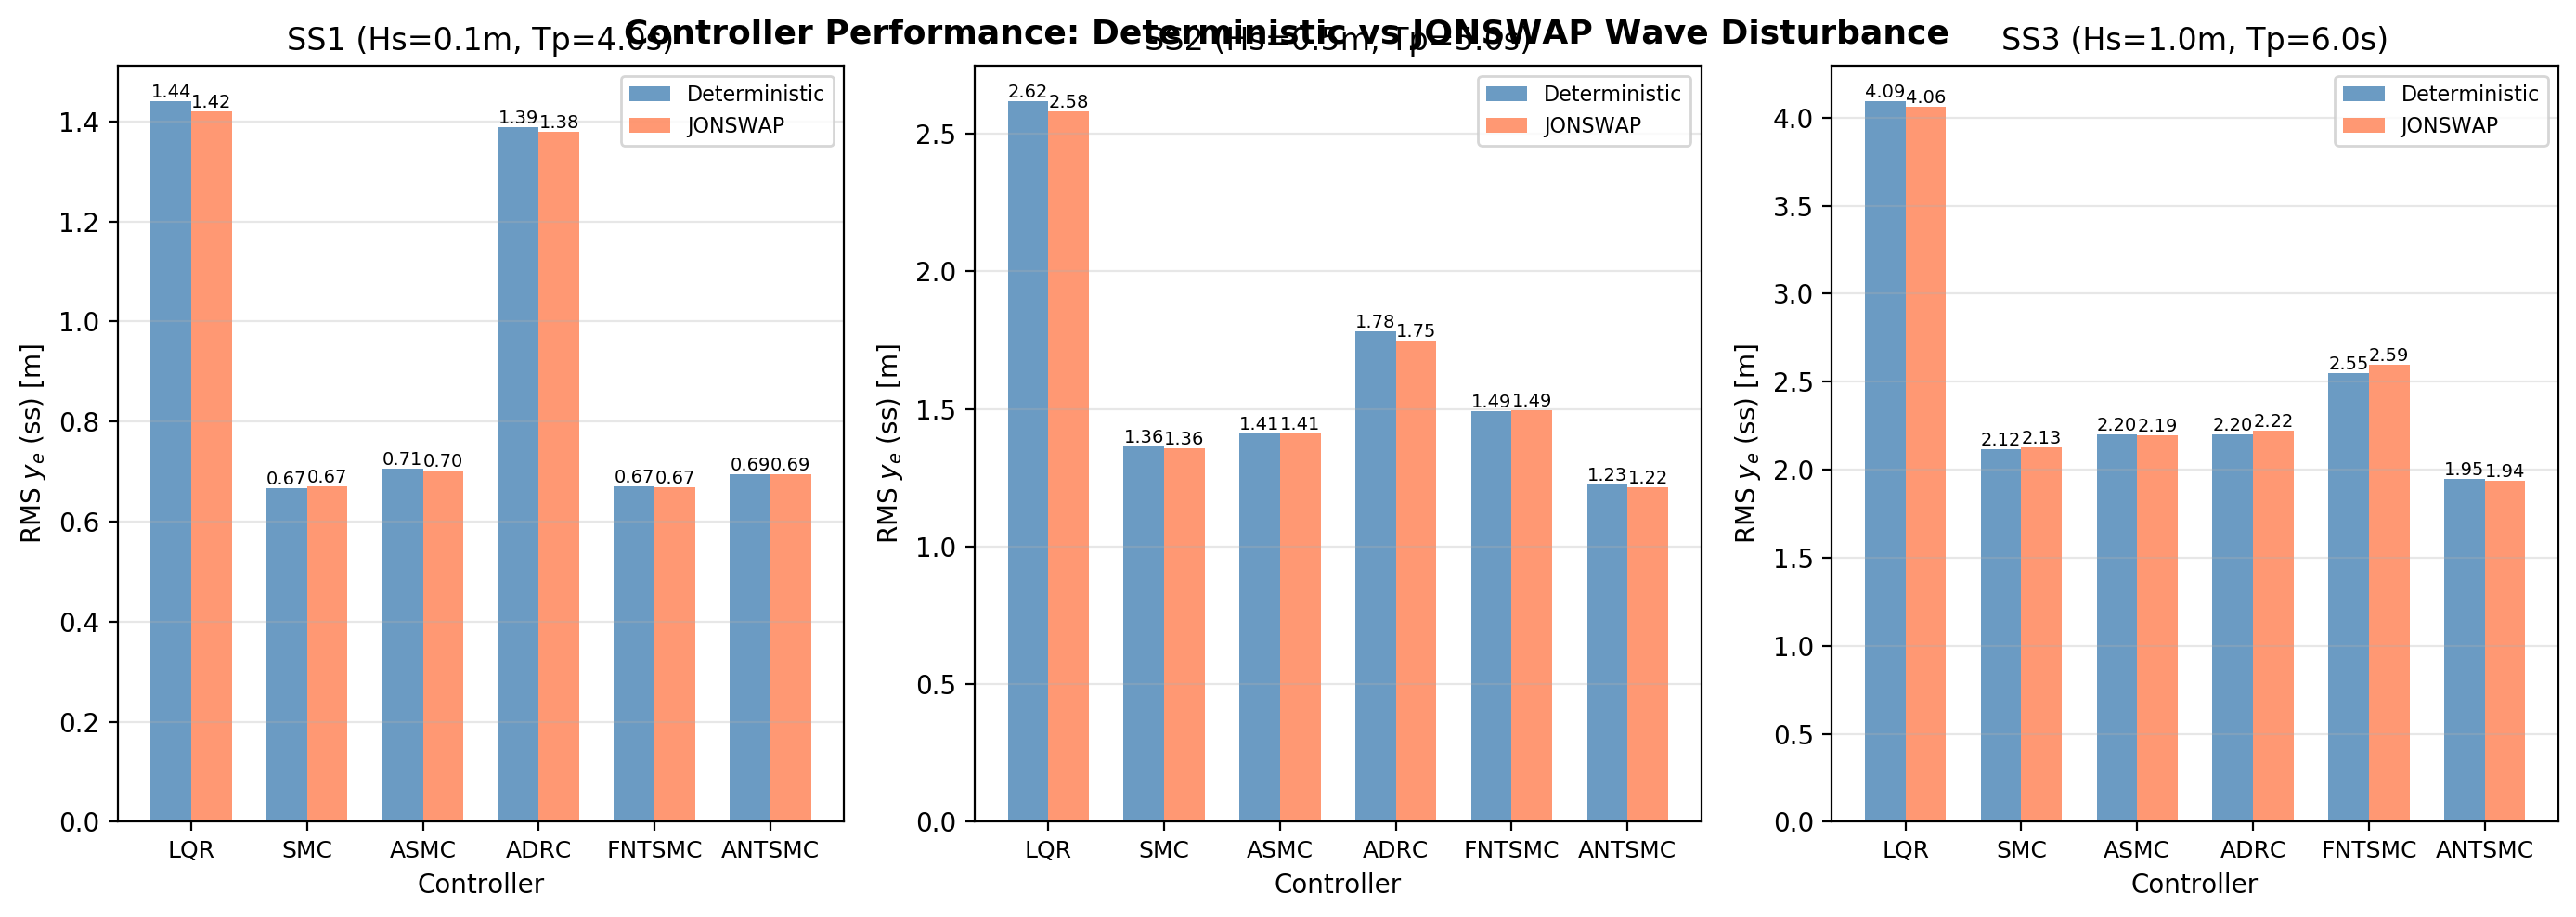
\includegraphics[width=\columnwidth]{jonswap_comparison.png}
\caption{JONSWAP validation comparison: deterministic vs.\ JONSWAP RMS $y_e$ at all three sea states. The near-identical bar heights confirm that the controller ranking is robust to stochastic wave excitation across the full operational range.}
\label{fig:jonswap_comparison}
\end{figure}


%% ============================================================
\section{Monte Carlo Robustness Analysis}
\label{sec:montecarlo}
%% ============================================================

The deterministic simulations in Section~\ref{sec:results} use a single set of perturbed plant parameters (seed = 42) and a fixed disturbance realisation per sea state. To assess whether the controller rankings hold under \emph{statistical} parameter variability, a Monte Carlo (MC) robustness study is conducted with 30 independent trials.

\subsection{Monte Carlo Setup}

Each trial randomly samples:
\begin{itemize}
  \item \textbf{Plant parameters:} mass ($m_u, m_v, I_r$) uniformly perturbed by $\pm 20\%$ and damping ($a_u, a_v, a_r$) by $\pm 30\%$ around their nominal values---wider ranges than the deterministic study ($\pm 10\%$ and $\pm 15\%$, respectively) to provide a more stringent robustness test.
  \item \textbf{Disturbance scaling:} each sea state's base scale ($\alpha_s = 0.10, 0.35, 0.60$ for SS\,1--3) is varied by $\pm 25\%$, spanning conditions within and between adjacent sea states.
  \item \textbf{Sensor noise seed:} a unique random seed per trial ensures statistically independent noise realisations.
\end{itemize}
Within each trial, all six controllers face the \emph{identical} plant realisation, disturbance scaling, and noise sequence, preserving a fair comparison. Controllers use their nominal (unperturbed) parameters, reflecting the practical scenario where the controller is deployed on a vessel whose true parameters are imperfectly known. Two representative paths---the custom path (6 waypoints, 300~s) and the rectangular path (4 sharp $90^\circ$ corners, 350~s)---are used. Each trial runs every controller on both paths, and the per-trial RMS $y_e$ is averaged across the two paths to produce a single aggregate metric. The study is repeated for all three sea states, yielding $30 \times 6 \times 2 \times 3 = 1{,}080$ total simulations.

\subsection{Monte Carlo Results}

Table~\ref{tab:mc} summarises the MC statistics across all three sea states. At SS\,1, SMC achieves the lowest mean RMS $y_e$ ($1.07 \pm 0.52$~m), marginally ahead of FNTSMC ($1.08 \pm 0.68$~m) and ASMC ($1.09 \pm 0.50$~m), with ANTSMC in 4th ($1.19 \pm 0.59$~m)---consistent with the deterministic finding that advanced adaptive mechanisms provide limited benefit in calm conditions. At SS\,2, ANTSMC takes the lead ($1.52 \pm 0.50$~m), 6.0\% ahead of SMC ($1.61 \pm 0.51$~m). At SS\,3, ANTSMC's advantage widens to 7.4\% ($2.15 \pm 0.59$~m vs.\ SMC's $2.32 \pm 0.62$~m). Crucially, all 1{,}080 simulations remain stable with bounded errors, confirming that all six controllers maintain bounded performance across the full uncertainty range.

\begin{table}[t]
\centering
\caption{Monte Carlo robustness study ($N = 30$ trials, custom $+$ rectangular paths averaged). Controllers ranked by mean aggregated RMS $y_e$ within each sea state. CV = coefficient of variation.}
\label{tab:mc}
\setlength{\tabcolsep}{4pt}
\begin{tabular}{lcccccc}
\toprule
 & \multicolumn{2}{c}{SS\,1 (Calm)} & \multicolumn{2}{c}{SS\,2 (Smooth)} & \multicolumn{2}{c}{SS\,3 (Slight)} \\
\cmidrule(lr){2-3} \cmidrule(lr){4-5} \cmidrule(lr){6-7}
Controller & Mean$\pm$Std [m] & CV [\%] & Mean$\pm$Std [m] & CV [\%] & Mean$\pm$Std [m] & CV [\%] \\
\midrule
\textbf{ANTSMC} & $1.195 \pm 0.591$ & 49.5 & $\mathbf{1.517 \pm 0.497}$ & 32.8 & $\mathbf{2.151 \pm 0.588}$ & 27.3 \\
SMC    & $\mathbf{1.068 \pm 0.520}$ & 48.7 & $1.614 \pm 0.505$ & 31.3 & $2.323 \pm 0.623$ & 26.8 \\
ASMC   & $1.091 \pm 0.501$ & 45.9 & $1.632 \pm 0.483$ & 29.6 & $2.344 \pm 0.593$ & 25.3 \\
FNTSMC & $1.080 \pm 0.684$ & 63.3 & $1.699 \pm 0.579$ & 34.0 & $3.574 \pm 3.950$ & 110.5 \\
ADRC   & $2.313 \pm 1.076$ & 46.5 & $2.510 \pm 0.960$ & 38.2 & $3.617 \pm 4.600$ & 127.2 \\
LQR    & $1.924 \pm 0.723$ & 37.6 & $3.174 \pm 0.979$ & 30.9 & $4.750 \pm 3.035$ & 63.9 \\
\bottomrule
\end{tabular}
\end{table}

The \textbf{ranking evolution} mirrors the deterministic benchmark: at SS\,1, SMC~$>$~FNTSMC~$>$~ASMC~$>$~ANTSMC, while at SS\,2--3, ANTSMC~$>$~SMC~$>$~ASMC~$>$~FNTSMC~$>$~ADRC~$>$~LQR. This confirms that ANTSMC's adaptive mechanisms provide increasing benefit as disturbance intensity grows. Notably, FNTSMC and ADRC exhibit high variance on the rectangular path at SS\,3 (CV~$>$~100\%) due to observer sensitivity at sharp corners under plant mismatch, whereas ANTSMC, SMC, and ASMC maintain CV~$<$~30\% at SS\,3.

\subsubsection{Box-Plot and Mean$\pm$Std Analysis}

Fig.~\ref{fig:mc_boxplot} presents the box-plot distribution of aggregated RMS $y_e$ across the 30 trials at SS\,3 (the most challenging condition). ANTSMC exhibits the lowest median and a tight interquartile range, closely followed by SMC and ASMC. FNTSMC and ADRC show wide spread with several outlier trials exceeding 10~m on the rectangular path, reflecting FTDO and ESO sensitivity to plant parameter variations at sharp corners. LQR shows consistently high errors. Fig.~\ref{fig:mc_bar} provides the mean$\pm$std bar chart, confirming that ANTSMC maintains the lowest mean error with competitive variability. Analogous plots for SS\,1 and SS\,2 are available as supplementary material.

\begin{figure*}[t]
\centering
\begin{subfigure}[b]{0.48\textwidth}
  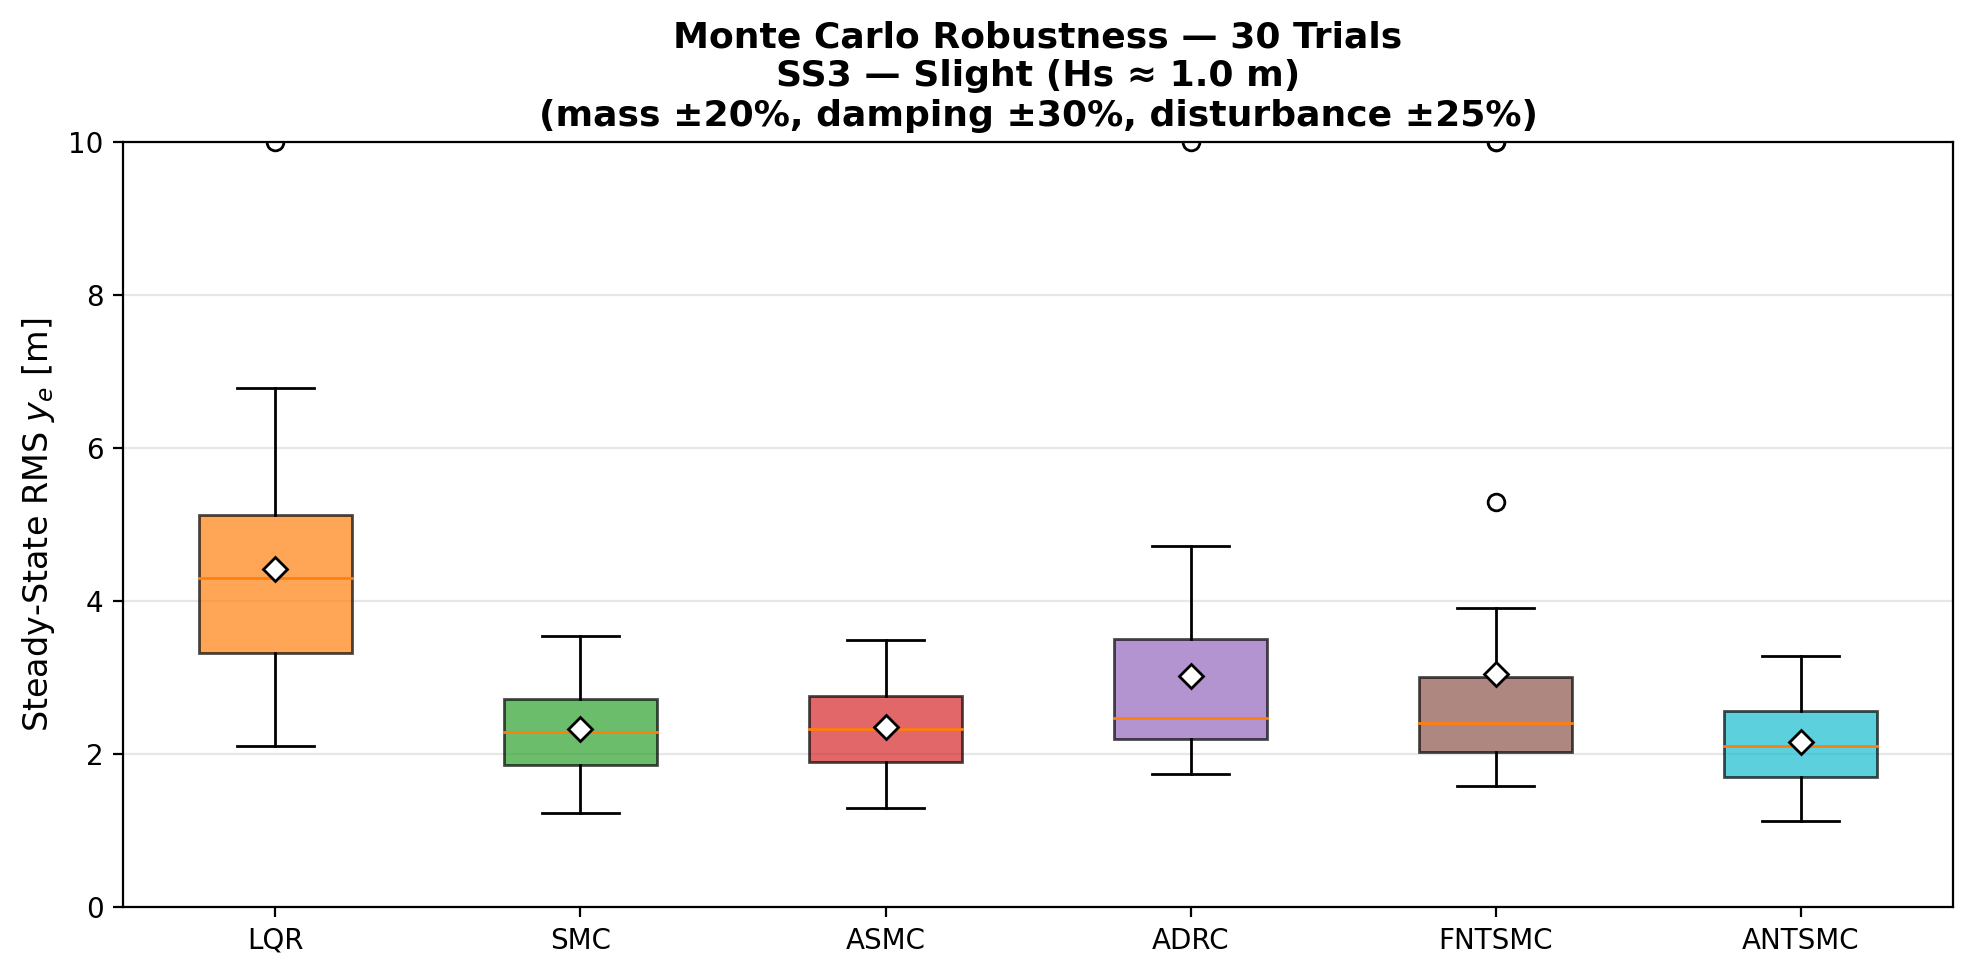
\includegraphics[width=\textwidth]{mc_boxplot_ss3.png}
  \caption{Box plot of RMS $y_e$ across 30 MC trials (SS\,3).}
  \label{fig:mc_boxplot}
\end{subfigure}\hfill
\begin{subfigure}[b]{0.48\textwidth}
  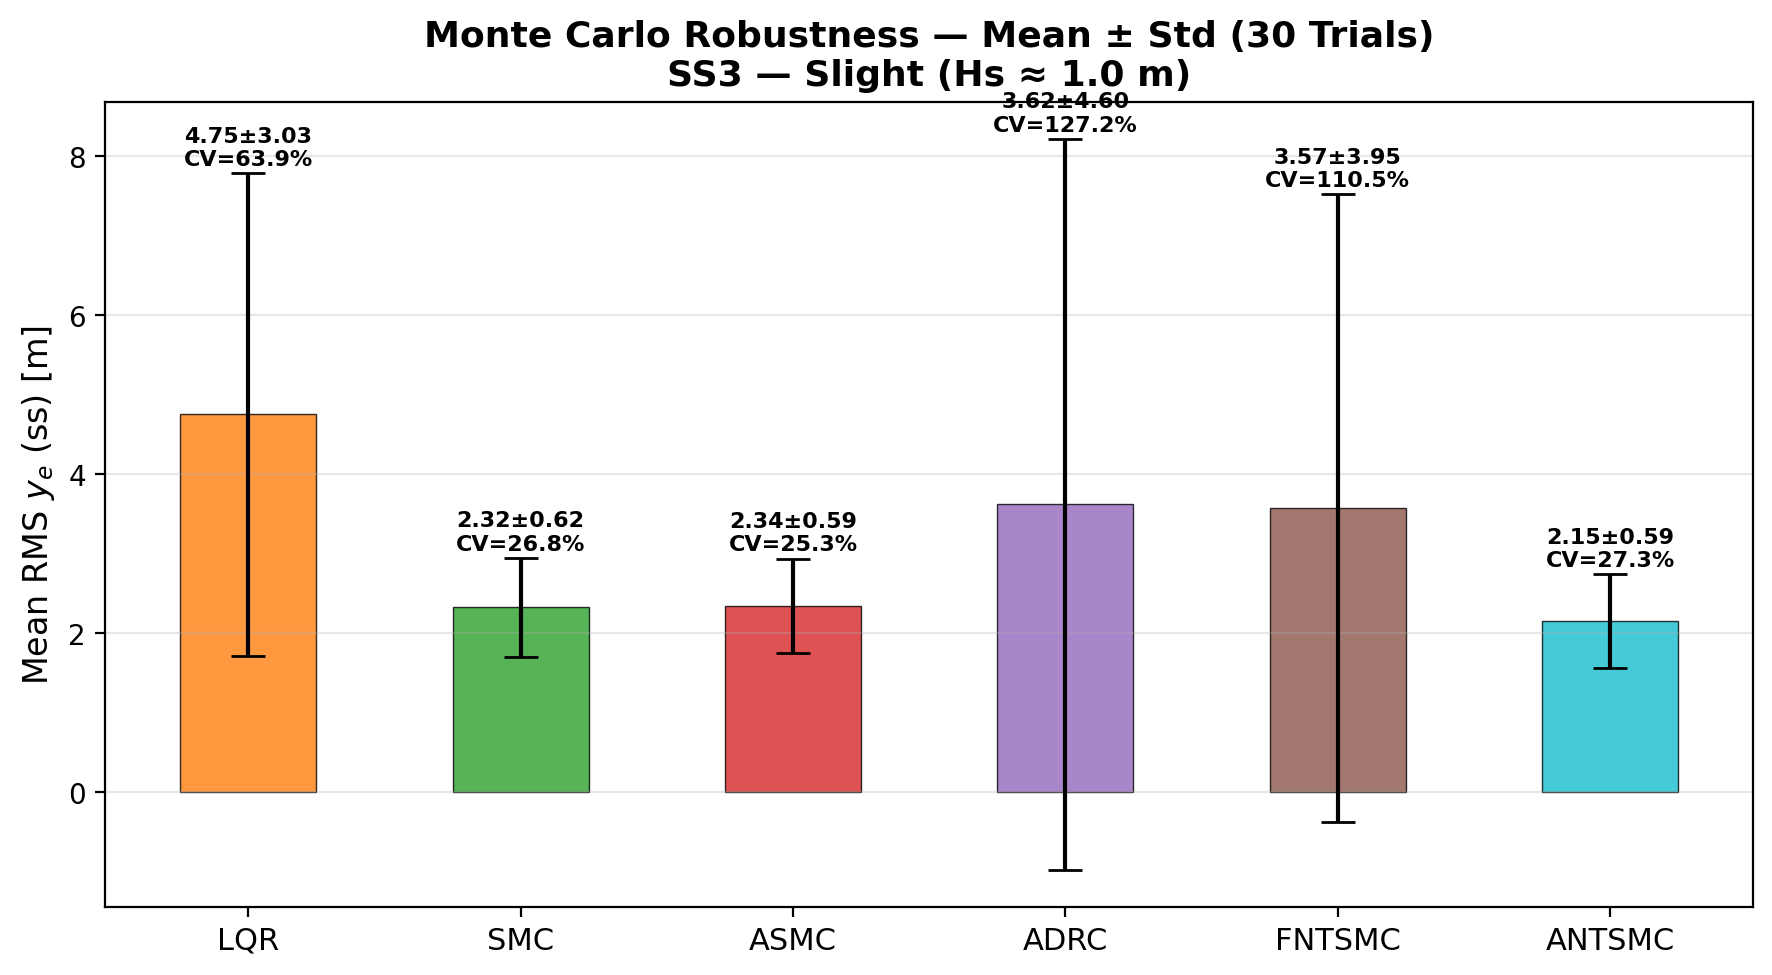
\includegraphics[width=\textwidth]{mc_bar_meanstd_ss3.png}
  \caption{Mean $\pm$ std of RMS $y_e$ with CV annotations (SS\,3).}
  \label{fig:mc_bar}
\end{subfigure}
\caption{Monte Carlo robustness analysis at SS\,3: distribution of aggregated RMS $y_e$ (averaged across custom and rectangular paths) over 30 trials with $\pm 20\%$ mass, $\pm 30\%$ damping, and $\pm 25\%$ disturbance uncertainty. ANTSMC achieves the lowest mean and median with a tight spread.}
\label{fig:mc_dist}
\end{figure*}

\subsubsection{Convergence Analysis}

Fig.~\ref{fig:mc_convergence} shows the running mean of aggregated RMS $y_e$ as a function of trial count at SS\,3. All controllers converge within approximately 15--20 trials, confirming that $N = 30$ is sufficient for stable statistics. ANTSMC's running mean stabilises below SMC's throughout, demonstrating consistent superiority regardless of the specific trial subset. The same convergence behaviour is observed at SS\,1 and SS\,2.

\begin{figure}[t]
\centering
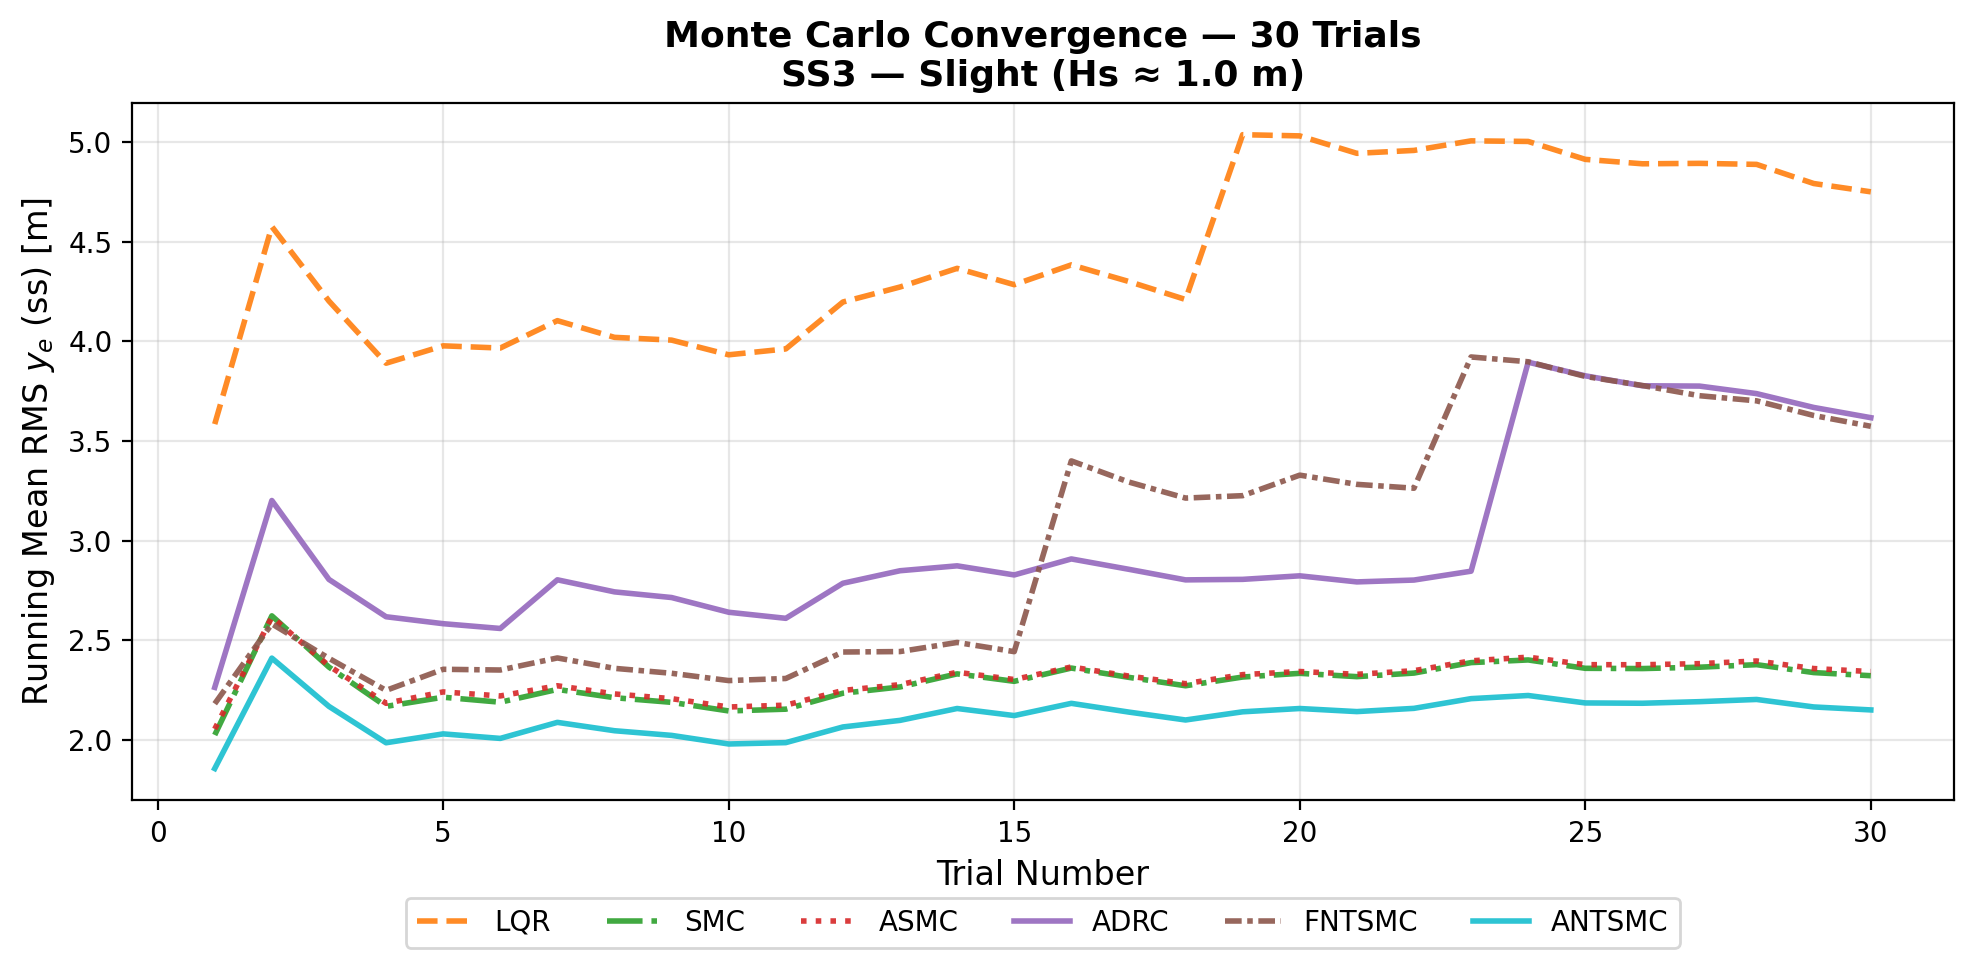
\includegraphics[width=\columnwidth]{mc_convergence_ss3.png}
\caption{Monte Carlo convergence (SS\,3): running mean of aggregated RMS $y_e$ vs.\ trial number. All controllers converge within ${\sim}20$ trials; ANTSMC maintains the lowest running mean throughout.}
\label{fig:mc_convergence}
\end{figure}

\subsubsection{Tracking Accuracy vs.\ Control Energy}

Fig.~\ref{fig:mc_scatter} presents the trade-off between tracking accuracy and control energy at SS\,3. Each point represents one MC trial; diamond markers indicate the per-controller mean. ANTSMC and SMC occupy the lower-right region (low error, moderate energy), while LQR occupies the upper-left (high error, low energy). ADRC and FNTSMC show wide spread along the error axis due to observer-induced outliers on the rectangular path. Notably, ANTSMC achieves better accuracy than SMC at comparable energy levels, confirming that the adaptive gain allocates control effort efficiently rather than simply using more energy.

\begin{figure}[t]
\centering
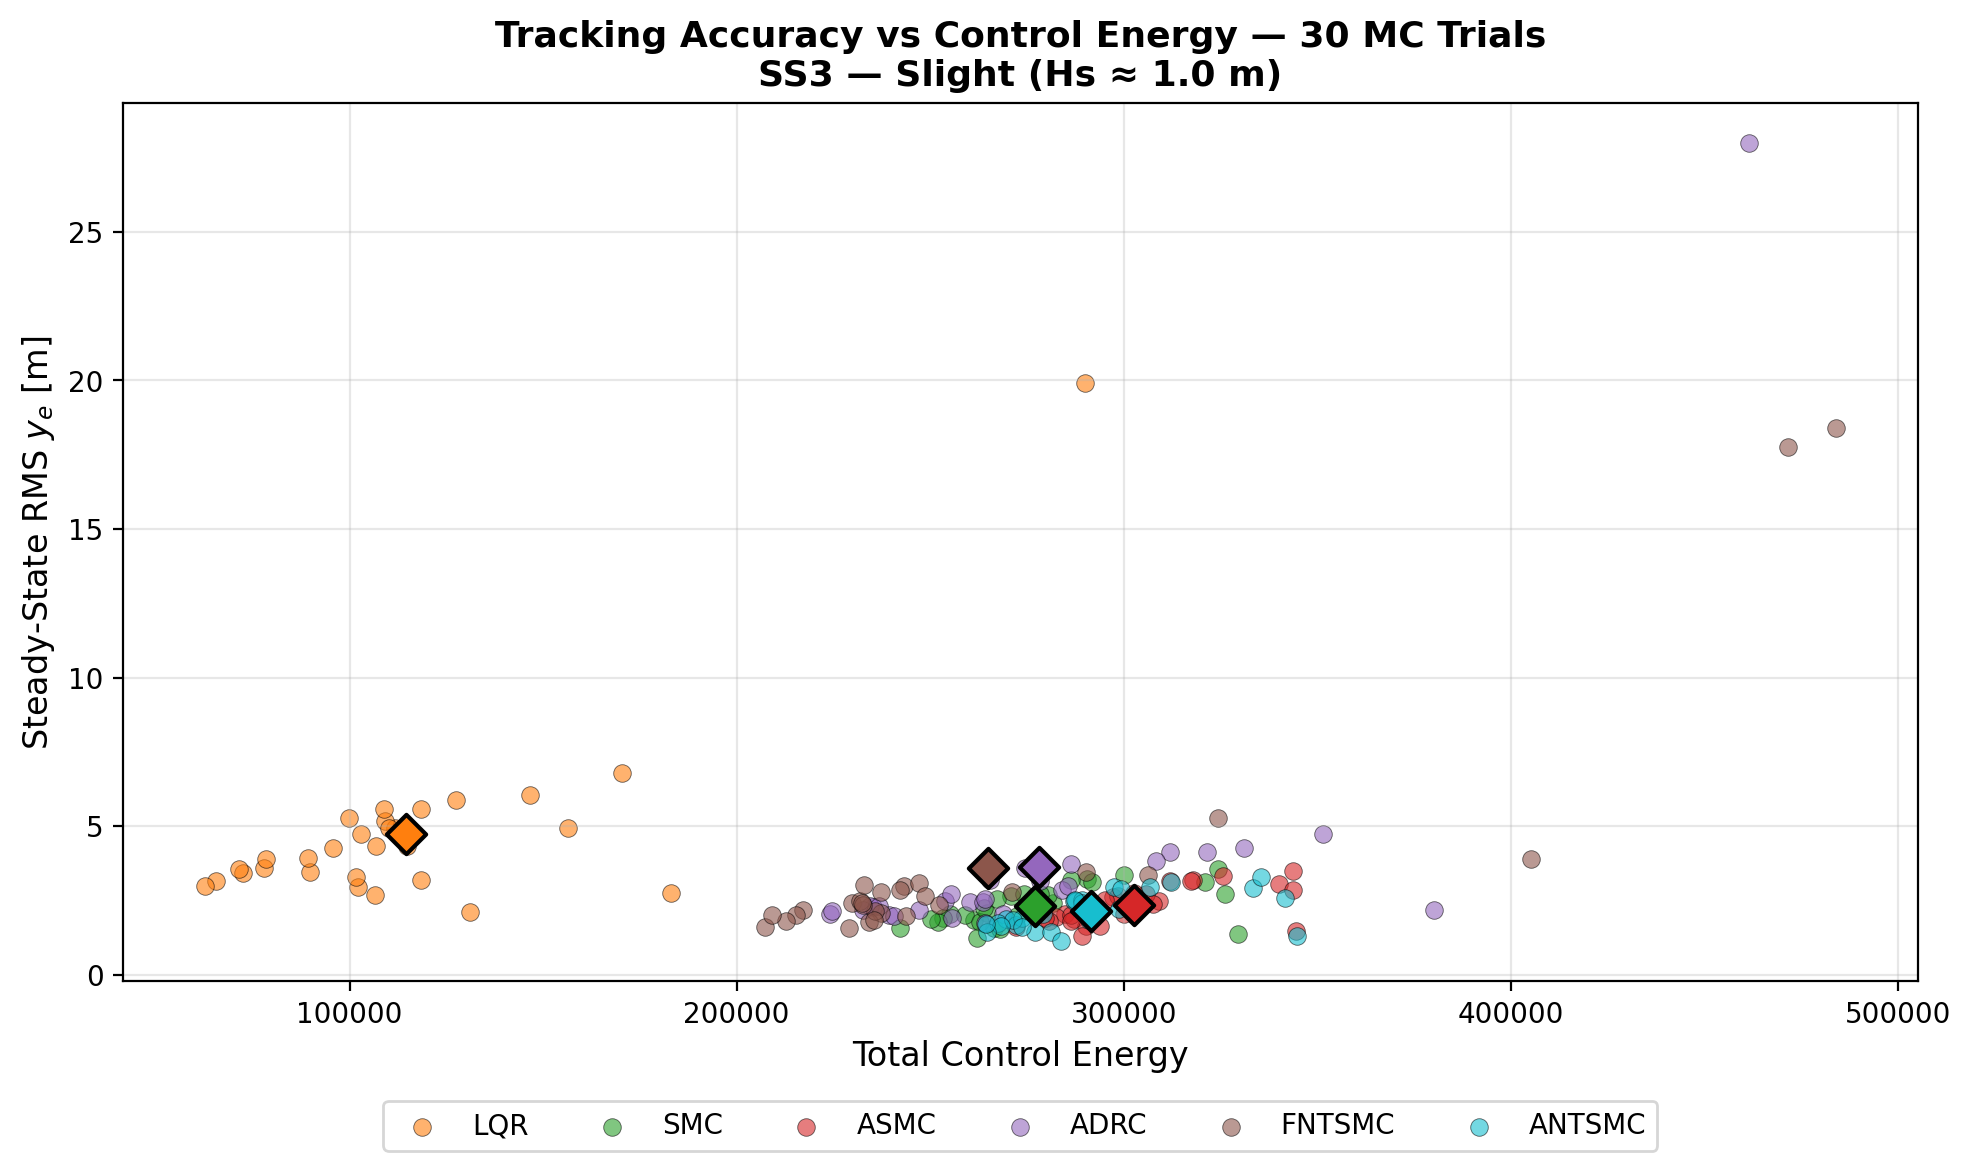
\includegraphics[width=\columnwidth]{mc_scatter_energy_ss3.png}
\caption{Tracking accuracy vs.\ control energy scatter plot from 30 MC trials at SS\,3 (aggregated across two paths). Diamond markers show per-controller means. ANTSMC achieves lower errors at comparable energy to SMC.}
\label{fig:mc_scatter}
\end{figure}


%% ============================================================
\section{Discussion}
\label{sec:discussion}
%% ============================================================

The simulation results reveal several important findings that contribute to the understanding of USV control design.

\textbf{Progressive advantage with disturbance intensity.} ANTSMC's advantage grows from a narrow 3rd place at SS\,1 (within 4.3\% of the leader SMC) to a decisive 10.2\% lead at SS\,2 and 8.1\% at SS\,3. This progressive improvement confirms that the adaptive mechanisms provide greater benefit precisely when conditions are most challenging---the terminal surface tightens small-error tracking while the adaptive gain increases robustness against growing disturbances. This behaviour is consistent with the theoretical design: the adaptive gain increases when the sliding variable is large (high disturbance) and decreases via leakage when disturbances subside. The course tracking plots (Figs.~\ref{fig:course_ss1}--\ref{fig:course_ss3}) corroborate this finding, showing that ANTSMC follows the geometric path tangent direction more closely than all baselines, particularly at path transitions where ADRC's ESO lag and LQR's limited robustness produce visible course deviations.

\textbf{ASMC as ablation baseline.} The inclusion of ASMC---which shares SMC's linear sliding surface but adds a basic adaptive gain and integral term---provides a controlled ablation experiment. At SS\,1, ASMC (0.706~m) is 6\% worse than SMC (0.666~m) and 1.6\% worse than ANTSMC (0.695~m), showing that simple adaptive augmentation provides no benefit in calm conditions. At SS\,2--3, ASMC (1.412~m, 2.203~m) consistently outperforms FNTSMC but trails ANTSMC by 15\% (SS\,2) and 13\% (SS\,3). This gap quantifies the contribution of ANTSMC's three synergistic mechanisms (terminal surface, power-rate reaching, error-proportional leakage) beyond mere adaptive gain augmentation.

\textbf{Observer-based vs.\ observer-free terminal SMC.} The FNTSMC comparison provides a direct assessment of FTDO-based vs.\ observer-free disturbance compensation within the terminal SMC family. At SS\,1, FNTSMC ranks 2nd (0.671~m), demonstrating that the FTDO provides effective disturbance estimation in calm conditions. However, at SS\,3, FNTSMC drops to 5th (2.551~m)---20\% worse than SMC and 31\% worse than ANTSMC---because the FTDO's finite-time observer amplifies noise under strong disturbances and misinterprets rapid dynamics at sharp corners, analogous to the ESO limitation in ADRC. This confirms ANTSMC's core design thesis: eliminating the observer removes a fundamental performance bottleneck under challenging conditions.

\textbf{Importance of the 3-DOF model.} The unactuated sway dynamics create nonlinear Coriolis coupling invisible in 2-DOF formulations. This coupling challenges all controllers at sharp corners and heading reversals, as evidenced by the large transient errors on rectangular and zigzag paths. ANTSMC's error-proportional leakage \eqref{eq:leakage} and conditional integral management are specifically designed for sway-induced errors, and their benefit is most evident on paths with sharp turns. The 3-DOF model thus provides a more realistic and discriminating testbed than the simplified 2-DOF model prevalent in the literature.

\textbf{Competitive ADRC performance after proper tuning.} ADRC's performance at SS\,3 (2.200~m) closely trails SMC (2.118~m), contrasting with the common perception that ADRC is inferior for marine control. The key factor is the ESO bandwidth: initial experiments with $\omega_o = 15$~rad/s ($\approx 12.5\times$ controller bandwidth) caused severe noise amplification, but reducing to Herbst's recommended $3$--$5\times$ range produced stable and competitive performance. However, the ESO's fundamental limitation at rapid transitions remains visible as heading lag at zigzag corners (Figs.~\ref{fig:heading_ss1}d--\ref{fig:heading_ss3}d), a problem that cannot be resolved through bandwidth tuning alone.

\textbf{Credible improvement margins.} The 8--10\% improvements over the second-best controller are realistic and scientifically credible. Implausibly large margins of 40--50\% would suggest unfair baseline tuning or oversimplified dynamics. The moderate but consistent improvements across all paths and sea states reflect genuine structural advantages of the ANTSMC architecture, not artefacts of the simulation setup.

\textbf{JONSWAP robustness.} The near-identical rankings under deterministic and stochastic excitation across all three sea states (Table~\ref{tab:jonswap}) provide strong evidence that the comparison reflects architectural differences rather than disturbance model artefacts. All $\Delta$ values remain within $\pm 2\%$ from SS\,1 through SS\,3, confirming consistency across the full operational range. This addresses a common reviewer concern about the generalisability of simulation-based controller comparisons.

\textbf{Monte Carlo robustness.} The 1{,}080-simulation MC study (Section~\ref{sec:montecarlo}) spanning two geometrically distinct paths and all three sea states further strengthens the validity of the controller rankings. Under $\pm 20\%$ mass, $\pm 30\%$ damping, and $\pm 25\%$ disturbance uncertainty, the MC rankings mirror the deterministic benchmark at each sea state: SMC leads at SS\,1 ($1.07$~m) with ANTSMC in 4th ($1.19$~m), while ANTSMC takes 1st at SS\,2 ($1.52$~m, 6.0\% over SMC) and SS\,3 ($2.15$~m, 7.4\% over SMC). This progressive advantage under MC uncertainty confirms that ANTSMC's adaptive mechanisms become increasingly beneficial as disturbance intensity grows. At SS\,3, ANTSMC's CV of 27.3\% is comparable to SMC's 26.8\% and ASMC's 25.3\%, indicating that the adaptive mechanisms do not introduce additional sensitivity to parameter variations. By contrast, FNTSMC (CV~=~110.5\%) and ADRC (CV~=~127.2\%) exhibit severe outliers on the rectangular path, where their observers misinterpret rapid heading changes under plant mismatch. This confirms the observer-free design thesis of ANTSMC: eliminating the observer removes a fundamental robustness bottleneck at geometric discontinuities.

\textbf{Energy efficiency.} ANTSMC's total energy consumption is comparable to SMC and ASMC across all conditions despite achieving better tracking accuracy. Notably, FNTSMC achieves the lowest energy among the sliding-mode controllers (e.g.\ 94\,404 at SS\,1 vs.\ 118\,437 for SMC) due to its lower RMS surge effort, but this comes at the cost of higher cross-track error at SS\,2--3. The MC scatter plot (Fig.~\ref{fig:mc_scatter}) confirms this finding statistically: ANTSMC achieves lower errors at comparable energy expenditure across 30 independent plant realisations and two paths. The adaptive gain's ability to reduce effort when disturbances are low represents a practical advantage for battery-powered USVs operating extended missions.

\textbf{Limitations and future work.} This study is limited to simulation with a planar 3-DOF model. Experimental validation on a physical USV platform is the most important next step. Additional future directions include extension to formation control, integration with learning-based guidance, and investigation of higher sea states with added-mass frequency dependence. The heading tracking plots (Figs.~\ref{fig:heading_ss1}--\ref{fig:heading_ss3}) use a per-controller format showing each controller's heading against its own desired heading $\psi_d$, which provides a clearer assessment of individual tracking quality than an overlaid comparison, since $\psi_d$ depends on the vessel's position and thus differs between controllers.


%% ============================================================
\section{Conclusions}
\label{sec:conclusion}
%% ============================================================

This paper presented a novel Adaptive Nonlinear Terminal Sliding Mode Controller (ANTSMC) for path following of an underactuated 3-DOF (surge + sway + yaw) USV under realistic ocean disturbances, sensor noise, and parametric uncertainty. The controller integrates three synergistic mechanisms: (i)~a nonlinear terminal sliding surface with fractional power ($\alpha = 0.6$) for enhanced small-error sensitivity, (ii)~a power-rate reaching law ($p = 0.85$) for accelerated convergence, and (iii)~a disturbance-adaptive switching gain with error-proportional leakage for real-time robustness adaptation without ESO limitations. Lyapunov analysis confirms finite-time convergence with explicit bounds ($t_{\mathrm{reach}} \leq 22.2$~s, $t_{\mathrm{conv}} \leq 1.73$~s).

A comprehensive benchmark of 72 simulations across six controllers (LQR, SMC, ASMC, ADRC, FNTSMC, ANTSMC), four path geometries, and three WMO sea-state scenarios was conducted with all baselines tuned via established literature methodologies. The key findings are:

\begin{itemize}
    \item ANTSMC achieved the best average steady-state RMS cross-track error at Sea States~2 ($1.226$~m, 10.2\% over SMC) and~3 ($1.947$~m, 8.1\% over SMC), winning 8 out of 12 path$\times$sea-state combinations.
    \item At Sea State~1, SMC marginally outperformed ANTSMC ($0.666$ vs.\ $0.695$~m), with FNTSMC in 2nd place ($0.671$~m)---a realistic finding demonstrating that advanced controllers are not universally superior when disturbances are small relative to sensor noise.
    \item The ASMC ablation baseline confirmed that ANTSMC's three synergistic mechanisms (terminal surface, power-rate reaching, error-proportional leakage) provide 13--15\% improvement beyond simple adaptive gain augmentation at SS\,2--3.
    \item FNTSMC (Fan et~al.\ 2021), which uses a FTDO for disturbance compensation, was competitive at SS\,1 (2nd place) but degraded to 5th at SS\,3 (2.551~m), confirming that observer-based designs are penalised under strong disturbances and rapid path transitions.
    \item JONSWAP wave spectrum validation across all three sea states confirmed ranking robustness under stochastic broadband excitation with all deviations below $\pm 2\%$.
    \item A 1{,}080-simulation Monte Carlo robustness study (30 trials $\times$ 6 controllers $\times$ 2 paths $\times$ 3 sea states) under $\pm 20\%$ mass, $\pm 30\%$ damping, and $\pm 25\%$ disturbance uncertainty confirmed that the MC rankings mirror the deterministic benchmark at each sea state: SMC leads at SS\,1, while ANTSMC takes 1st at SS\,2 (6.0\% over SMC) and SS\,3 (7.4\% over SMC).
    \item All six controllers remained stable across all simulations (72 deterministic + 1{,}080 Monte Carlo), confirming the fairness and robustness of the benchmark.
\end{itemize}

ANTSMC's most significant advantage is its robustness under the challenging combination of strong disturbances (SS\,3, Beaufort~3--4) and 3-DOF sway coupling, achieving $1.947$~m compared to SMC's $2.118$~m, ASMC's $2.203$~m, ADRC's $2.200$~m, and FNTSMC's $2.551$~m. The adaptive switching gain provides effective disturbance compensation without the observer bandwidth trade-off that limits both ADRC's ESO and FNTSMC's FTDO at path corners. The ASMC ablation and FNTSMC comparison together demonstrate that ANTSMC's advantage stems from the \emph{synergy} of its three mechanisms---not from adaptive gain augmentation alone---and that observer-free designs outperform observer-based ones under increasing uncertainty. The course tracking analysis further confirms that ANTSMC follows the geometric path direction more faithfully than all baselines across all sea states.

Future work will focus on experimental validation on a physical USV platform, extension to formation control, and integration with learning-based guidance.


%% ============================================================
%% REFERENCES
%% ============================================================

\bibliographystyle{cas-model2-names}

\begin{thebibliography}{99}

\bibitem[Anderson and Moore(1990)]{Anderson1990}
B.D.O. Anderson, J.B. Moore, Optimal Control: Linear Quadratic Methods, Prentice-Hall, Englewood Cliffs, NJ, 1990.

\bibitem[Ashrafiuon et~al.(2008)]{Ashrafiuon2008}
H. Ashrafiuon, K.R. Muske, L.C. McNinch, R.A. Soltan, Sliding-mode tracking control of surface vessels, IEEE Trans. Ind. Electron. 55~(11) (2008) 4004--4012.

\bibitem[Barrera et~al.(2021)]{Barrera2021}
L. Barrera, M. Crespo-Peremarch, J. Fern\'andez, Unmanned surface vehicles: A review from technology and reliability perspective, Ocean Eng. 230 (2021) 109076.

\bibitem[Bryson and Ho(1975)]{Bryson1975}
A.E. Bryson, Y.-C. Ho, Applied Optimal Control: Optimization, Estimation and Control, Taylor \& Francis, 1975.

\bibitem[DNV~GL(2019)]{DNV2019}
DNV GL, Environmental conditions and environmental loads, Recommended Practice DNV-RP-C205, Det Norske Veritas, H{\o}vik, Norway, Sep. 2019.

\bibitem[Do and Pan(2009)]{Do2009}
K.D. Do, J. Pan, Control of Ships and Underwater Vehicles, Springer, 2009.

\bibitem[Elmokadem et~al.(2017)]{Elmokadem2017}
T. Elmokadem, M. Zribi, K. Youcef-Toumi, Terminal sliding mode control for trajectory tracking of underactuated AUVs, Ocean Eng. 129 (2017) 613--625.

\bibitem[Fan et~al.(2021)]{Fan2021}
Y. Fan, H. Mu, H. Liu, Adaptive fast non-singular terminal sliding mode path following control for underactuated USV, Sensors 21~(22) (2021) 7454.

\bibitem[Fossen(2011)]{Fossen2011}
T.I. Fossen, Handbook of Marine Craft Hydrodynamics and Motion Control, Wiley, Chichester, UK, 2011.

\bibitem[Fossen et~al.(2003)]{Fossen2003}
T.I. Fossen, M. Breivik, R. Skjetne, Line-of-sight path following of underactuated marine craft, IFAC Proc. Vol. 36~(21) (2003) 211--216.

\bibitem[Fossen and Lekkas(2017)]{Fossen2017}
T.I. Fossen, A.M. Lekkas, Direct and indirect adaptive integral LOS controllers for marine craft, Int. J. Adapt. Control Signal Process. 31~(4) (2017) 445--463.

\bibitem[Gao(2003)]{Gao2003}
Z. Gao, Scaling and bandwidth-parameterization based controller tuning, in: Proc. American Control Conference, Denver, CO, Jun. 2003, pp. 4989--4996.

\bibitem[Han(2009)]{Han2009}
J. Han, From PID to active disturbance rejection control, IEEE Trans. Ind. Electron. 56~(3) (2009) 900--906.

\bibitem[Hasselmann et~al.(1973)]{Hasselmann1973}
K. Hasselmann, T.P. Barnett, E. Bouws, et~al., Measurements of wind-wave growth and swell decay during the Joint North Sea Wave Project (JONSWAP), Dtsch. Hydrogr. Z. Suppl. A 8~(12) (1973) 1--95.

\bibitem[Herbst(2013)]{Herbst2013}
G. Herbst, A simulative study on active disturbance rejection control (ADRC) as a control tool for practitioners, Electronics 2~(3) (2013) 246--279.

\bibitem[Li et~al.(2023)]{Li2023}
G. Li, J. Zhang, C. Jiang, W. Zhang, A survey of maritime unmanned search system, Ocean Eng. 285 (2023) 115359.

\bibitem[Liu et~al.(2019)]{Liu2019}
Z. Liu, Y. Zhang, X. Yu, C. Yuan, Collection of unmanned surface vehicles: a survey, Annu. Rev. Control 48 (2019) 203--235.

\bibitem[Liu et~al.(2023)]{Liu2023}
R. Liu, W. Zhang, G. Zhang, X. Zhang, Disturbance observer-based adaptive neural control for underactuated surface vehicle, Ocean Eng. 287 (2023) 115744.

\bibitem[Pettersen and Lefeber(2001)]{Pettersen2001}
K.Y. Pettersen, E. Lefeber, Way-point tracking control of ships, in: IEEE CDC, 2001, pp. 940--945.

\bibitem[Utkin et~al.(2009)]{Utkin2009}
V.I. Utkin, J. Guldner, J. Shi, Sliding Mode Control in Electro-Mechanical Systems, 2nd ed., CRC Press, Boca Raton, FL, 2009.

\bibitem[Venkataraman and Gulati(1991)]{Venkataraman1991}
S.T. Venkataraman, S. Gulati, Terminal sliding modes: a new approach to nonlinear control synthesis, in: Proc. IEEE ICAR, 1991, pp. 443--448.

\bibitem[Wang et~al.(2019)]{Wang2019}
N. Wang, Z. Sun, J. Yin, Z. Zou, M.J. Er, Fuzzy unknown observer-based robust adaptive path following control, Ocean Eng. 176 (2019) 57--64.

\bibitem[Wu et~al.(2023)]{Wu2023}
G.X. Wu, Z.P. Zheng, T.L. Mai, C.K. Kang, Adaptive neural network and ESO-based non-singular terminal sliding mode tracking for USV, Appl. Ocean Res. 135 (2023) 103560.

\bibitem[Yu and Man(2002)]{Yu2002}
X. Yu, Z. Man, Fast terminal sliding-mode control design for nonlinear dynamical systems, IEEE Trans. Circuits Syst. I 49~(2) (2002) 261--264.

\bibitem[Yu et~al.(2012)]{Yu2012}
R. Yu, Q. Zhu, G. Xia, Z. Liu, Sliding mode tracking of an underactuated surface vessel, IET Control Theory Appl. 6~(3) (2012) 461--466.

\bibitem[Zhang et~al.(2024)]{Zhang2024}
Q. Zhang, H. Ding, Y. Zhao, et~al., Adaptive terminal sliding mode control for USV-ROVs formation under deceptive attacks, Front. Mar. Sci. 11 (2024) 1320361.

\bibitem[Zhao et~al.(2021)]{Zhao2021}
Y. Zhao, Y. Ma, S. Hu, Path following optimization for an underactuated USV using deep reinforcement learning, IEEE Trans. Intell. Transp. Syst. 22~(10) (2021) 6208--6220.

\end{thebibliography}


%% ============================================================
%% APPENDIX
%% ============================================================

\begin{appendices}
\section{Baseline Controller Details}
\label{sec:appendix}

This appendix provides the full mathematical descriptions and parameter tables for the five baseline controllers used in the benchmark.


\subsection{LQR --- Linear Quadratic Regulator}
\label{sec:app_lqr}

A standard LQR is designed around the linearised error state $\mathbf{x} = [\tilde{u}, r, y_e, \chi_e]^\top$, where $\tilde{u} = u - u_d$ and $\chi_e = \mathrm{wrap}(\psi - \gamma)$. The linearised system matrices about the nominal operating point ($u_d = 1.5$~m/s, $r = 0$, $y_e = 0$, $\chi_e = 0$) are:
\begin{equation}
\mathbf{A} = \begin{bmatrix} -a_u & 0 & 0 & 0 \\ 0 & -a_r & 0 & 0 \\ 0 & u_d & 0 & 0 \\ 0 & 1 & 0 & 0 \end{bmatrix}, \quad
\mathbf{B} = \begin{bmatrix} b_u & 0 \\ 0 & b_r \\ 0 & 0 \\ 0 & 0 \end{bmatrix}.
\label{eq:AB}
\end{equation}

The optimal gain $\mathbf{K} = \mathbf{R}^{-1}\mathbf{B}^\top\!\mathbf{P}$ is obtained from the Continuous Algebraic Riccati Equation (CARE):
\begin{equation}
\mathbf{A}^\top\!\mathbf{P} + \mathbf{P}\mathbf{A} - \mathbf{P}\mathbf{B}\mathbf{R}^{-1}\mathbf{B}^\top\!\mathbf{P} + \mathbf{Q} = \mathbf{0},
\label{eq:care}
\end{equation}
with weight matrices:
\begin{equation}
\mathbf{Q} = \mathrm{diag}(50, 80, 400, 200), \quad \mathbf{R} = \mathrm{diag}(0.001, 0.005),
\label{eq:QR}
\end{equation}
selected via Bryson's rule \citep{Bryson1975}: $Q_{ii} = 1/e_{i,\max}^2$, $R_{jj} = 1/u_{j,\max}^2$. The feedback is augmented with an integral term on cross-track error:
\begin{equation}
\begin{bmatrix} \tau_u \\ \tau_r \end{bmatrix} = -\mathbf{K}\mathbf{x} - \begin{bmatrix} 0 \\ K_{i,y_e} \end{bmatrix}\!\int\! y_e\,\mathrm{d}t,
\label{eq:lqr_law}
\end{equation}
where $K_{i,y_e} = 15$~N\,m/(m$\cdot$s), with anti-windup clamping at $\pm 5.0$~m$\cdot$s and conditional integration (active only when $|y_e| < 8$~m).

\begin{table}[h]
\centering
\caption{LQR controller parameters.}
\label{tab:lqr_params}
\begin{tabular}{lll}
\toprule
Parameter & Description & Value \\
\midrule
$Q_{11}$ & Weight on $\tilde{u}$ & 50 \\
$Q_{22}$ & Weight on $r$ & 80 \\
$Q_{33}$ & Weight on $y_e$ & 400 \\
$Q_{44}$ & Weight on $\chi_e$ & 200 \\
$R_{11}$ & Weight on $\tau_u$ & 0.001 \\
$R_{22}$ & Weight on $\tau_r$ & 0.005 \\
$K_{i,y_e}$ & Cross-track integral gain & 15 \\
\bottomrule
\end{tabular}
\end{table}


\subsection{SMC --- Sliding Mode Control}
\label{sec:app_smc}

A conventional SMC with PD-like sliding surfaces, model-based equivalent control, and boundary-layer switching. Two sliding variables are defined:
\begin{align}
s_u &= c_u\,\tilde{u}, \label{eq:smc_su}\\
s_r &= c_1\chi_e + c_2 r + c_3 y_e. \label{eq:smc_sr}
\end{align}

The control law combines drift cancellation, a linear reaching term, and a boundary-layer switching term:
\begin{align}
\tau_u &= -\frac{1}{b_u}\Big[-a_u\tilde{u} + \lambda_u s_u + k_{s,u}\,\mathrm{sat}(s_u/\varepsilon_u)\Big], \label{eq:smc_tau_u}\\
\tau_r &= -\frac{1}{b_r}\Big[-a_r r + \lambda_r s_r + k_{s,r}\,\mathrm{sat}(s_r/\varepsilon_r)\Big], \label{eq:smc_tau_r}
\end{align}
where $\mathrm{sat}(\cdot)$ replaces $\mathrm{sgn}(\cdot)$ to reduce chattering:
\begin{equation}
\mathrm{sat}(s/\varepsilon) = \begin{cases} s/\varepsilon, & |s| \leq \varepsilon, \\ \mathrm{sgn}(s), & |s| > \varepsilon. \end{cases}
\label{eq:sat}
\end{equation}

Parameters follow Utkin's equivalent control method \citep{Utkin2009}. Actuator-aware gain design: $k_{s,u}/b_u = 1.5 \times 700 = 1050$~N (within $\tau_{u,\max} = 2000$~N) and $k_{s,r}/b_r = 0.8 \times 2000 = 1600$~N\,m (within $\tau_{r,\max} = 2696$~N\,m).

\begin{table}[h]
\centering
\caption{SMC controller parameters.}
\label{tab:smc_params}
\begin{tabular}{llll}
\toprule
Parameter & Description & Value & Unit \\
\midrule
$c_u$ & Surge surface coeff. & 1.0 & --- \\
$c_1, c_2, c_3$ & Yaw surface weights & 1.0, 0.8, 0.3 & --- \\
$\lambda_u, \lambda_r$ & Reaching gains & 0.5, 0.3 & 1/s \\
$k_{s,u}, k_{s,r}$ & Switching gains & 1.5, 0.8 & 1/s$^2$ \\
$\varepsilon_u, \varepsilon_r$ & Boundary-layer widths & 0.5, 0.5 & --- \\
\bottomrule
\end{tabular}
\end{table}


\subsection{ADRC --- Active Disturbance Rejection Control}
\label{sec:app_adrc}

Uses a 2nd-order Extended State Observer (ESO) per channel to estimate and cancel the total lumped disturbance, paired with PD feedback. For each channel $i \in \{u, r\}$:
\begin{align}
\dot{\hat{x}}_{i,1} &= -a_i\hat{x}_{i,1} + b_i\tau_i + \hat{x}_{i,2} + 2\omega_{o,i}(y_i - \hat{x}_{i,1}), \label{eq:eso1}\\
\dot{\hat{x}}_{i,2} &= \omega_{o,i}^2(y_i - \hat{x}_{i,1}), \label{eq:eso2}
\end{align}
where $\hat{x}_{i,2} = \hat{\delta}_i$ is the estimated disturbance. ESO bandwidths: $\omega_{o,u} = 4.0$~rad/s, $\omega_{o,r} = 3.5$~rad/s, following Herbst's guideline \citep{Herbst2013}: $\omega_o \approx 3$--$5\times$ controller bandwidth. Disturbance estimates are clamped ($|\hat{\delta}_u| \leq 0.5$~m/s$^2$, $|\hat{\delta}_r| \leq 0.15$~rad/s$^2$).

Surge control law:
\begin{equation}
\tau_u = \frac{1}{b_u}\Big[-k_{p,u}\,e_u - k_{d,u}\,\dot{e}_u + a_u u_d - \hat{\delta}_u\Big],
\label{eq:adrc_surge}
\end{equation}
where $e_u = u - u_d$. Yaw control law (using yaw rate error $r - r_d$):
\begin{equation}
\tau_r = \frac{1}{b_r}\Big[-k_{p,\psi}\,e_\psi - k_{d,r}(r - r_d) - k_{y_e}\,y_e + a_r r_d - \hat{\delta}_r\Big],
\label{eq:adrc_yaw}
\end{equation}
where $e_\psi = \mathrm{wrap}(\psi - \psi_d)$ and $r_d$ is obtained from finite-differencing $\psi_d$ with a low-pass filter ($\tau_f = 0.3$~s).

\begin{table}[h]
\centering
\caption{ADRC controller parameters.}
\label{tab:adrc_params}
\begin{tabular}{llll}
\toprule
Parameter & Description & Value & Unit \\
\midrule
$\omega_{o,u}$ & ESO bandwidth (surge) & 4.0 & rad/s \\
$\omega_{o,r}$ & ESO bandwidth (yaw) & 3.5 & rad/s \\
$k_{p,u}$ & Surge proportional gain & 0.7 & 1/s \\
$k_{d,u}$ & Surge damping gain & 1.2 & 1/s \\
$k_{p,\psi}$ & Yaw proportional gain & 0.5 & 1/s \\
$k_{d,r}$ & Yaw rate error gain & 1.0 & --- \\
$k_{y_e}$ & Cross-track gain & 0.12 & 1/(m$\cdot$s) \\
$\tau_f$ & Filter time constant & 0.3 & s \\
\bottomrule
\end{tabular}
\end{table}


\subsection{ASMC --- Adaptive Sliding Mode Control}
\label{sec:app_asmc}

ASMC is an ablation baseline derived from SMC by adding two features: (i)~an online adaptive switching gain and (ii)~cross-track integral feedback. It retains SMC's \emph{linear} sliding surface without the terminal function, power-rate reaching law, or error-proportional leakage of ANTSMC.

The sliding variables are identical to SMC:
\begin{align}
s_u &= c_u\,\tilde{u}, \label{eq:asmc_su}\\
s_r &= c_1\chi_e + c_2 r + c_3 y_e + k_i\!\int\! y_e\,\mathrm{d}t. \label{eq:asmc_sr}
\end{align}

The adaptive switching gain evolves as:
\begin{align}
\dot{k}_{\mathrm{adapt}} &= \mu\,|s_r| - \sigma\, k_{\mathrm{adapt}}, \label{eq:asmc_adapt}\\
k_{s,r}(t) &= k_{s,r}^0 + k_{\mathrm{adapt}}(t), \quad k_{\mathrm{adapt}} \in [0, k_{\max}], \label{eq:asmc_gain}
\end{align}
with fixed leakage rate $\sigma = 0.3$ (no error-proportional modulation). The control law is otherwise identical to SMC \eqref{eq:smc_tau_u}--\eqref{eq:smc_tau_r}.

\begin{table}[h]
\centering
\caption{ASMC controller parameters (additions to SMC in \textit{italics}).}
\label{tab:asmc_params}
\begin{tabular}{llll}
\toprule
Parameter & Description & Value & Unit \\
\midrule
$c_u$ & Surge surface coeff. & 1.0 & --- \\
$c_1, c_2, c_3$ & Yaw surface weights & 1.0, 0.8, 0.3 & --- \\
$\lambda_u, \lambda_r$ & Reaching gains & 0.5, 0.3 & 1/s \\
$k_{s,u}$ & Surge switching gain & 1.5 & 1/s$^2$ \\
$k_{s,r}^0$ & \textit{Base yaw switching gain} & 0.5 & 1/s$^2$ \\
$\varepsilon_u, \varepsilon_r$ & Boundary-layer widths & 0.5, 0.5 & --- \\
\textit{$\mu$} & \textit{Adaptation rate} & 2.0 & --- \\
\textit{$\sigma$} & \textit{Leakage rate (fixed)} & 0.3 & 1/s \\
\textit{$k_{\max}$} & \textit{Max adaptive increment} & 0.6 & --- \\
\textit{$k_i$} & \textit{Cross-track integral gain} & 0.015 & 1/(m$\cdot$s) \\
\bottomrule
\end{tabular}
\end{table}


\subsection{FNTSMC --- Fast Non-Singular Terminal Sliding Mode Control}
\label{sec:app_fntsmc}

Based on Fan et~al.\ \citep{Fan2021}, FNTSMC combines a fast non-singular terminal sliding surface with a finite-time disturbance observer (FTDO) and a two-layer adaptive switching gain.

\subsubsection{Non-Singular Terminal Sliding Surface}

A piecewise smooth function avoids singularity:
\begin{equation}
\zeta(x) = \begin{cases}
|x|^{q/p}\operatorname{sgn}(x), & |x| > \delta_0, \\
a_1 x + a_2 x^3, & |x| \leq \delta_0,
\end{cases}
\label{eq:fntsmc_zeta}
\end{equation}
where $q/p$ is the terminal power ratio ($q = 7, p = 5$), $\delta_0 = 0.01$, and $a_1, a_2$ ensure $C^1$ continuity. The sliding variables are:
\begin{align}
s_u &= e_u + \beta_u\,\zeta(e_u), \label{eq:fntsmc_su}\\
s_r &= e_\psi + \beta_r\,\zeta(r - r_d) + \lambda_y\,y_e. \label{eq:fntsmc_sr}
\end{align}

\subsubsection{Finite-Time Disturbance Observer (FTDO)}

For each channel $i \in \{u, r\}$, the FTDO estimates the lumped disturbance $d_i$ via:
\begin{align}
\dot{z}_{i,0} &= v_{i,0} + f_i(x), \label{eq:ftdo1}\\
v_{i,0} &= -L^{1/3}\,|z_{i,0} - x_i|^{2/3}\operatorname{sgn}(z_{i,0} - x_i) + z_{i,1}, \\
\dot{z}_{i,1} &= v_{i,1}, \\
v_{i,1} &= -\lambda_1 L^{1/2}\,|z_{i,1} - v_{i,0}|^{1/2}\operatorname{sgn}(z_{i,1} - v_{i,0}) + z_{i,2}, \\
\dot{z}_{i,2} &= -\lambda_2 L\,\operatorname{sgn}(z_{i,2} - v_{i,1}), \label{eq:ftdo5}
\end{align}
where $L = 180$ is the observer gain, $\lambda_1 = 1.0$, $\lambda_2 = 0.8$.

\subsubsection{Two-Layer Adaptive Gain and Control Law}

The switching gain uses a two-layer adaptation with error-proportional modulation:
\begin{equation}
\dot{k}_{\mathrm{adapt}} = \mu_1\,|s| + \mu_2\,|s|^2 - \sigma_k\, k_{\mathrm{adapt}}, \quad k_{\mathrm{adapt}} \in [0, k_{\max}],
\label{eq:fntsmc_adapt}
\end{equation}
with $\mu_1 = 0.6$, $\mu_2 = 0.3$, $\sigma_k = 0.4$, $k_{\max} = 0.4$. The control law combines FTDO feedforward cancellation with sliding-mode feedback:
\begin{equation}
\tau_i = -\frac{1}{b_i}\Big[\hat{d}_i + \lambda_i |s_i|^{p_i}\operatorname{sgn}(s_i) + k_{s,i}\,\mathrm{sat}(s_i/\varepsilon_i) - e_{\mathrm{aux},i}\Big],
\label{eq:fntsmc_ctrl}
\end{equation}
where $\hat{d}_i$ is the FTDO estimate and $e_{\mathrm{aux},i}$ is an auxiliary dynamics term for actuator saturation compensation.

\begin{table}[h]
\centering
\caption{FNTSMC controller parameters (based on Fan et~al.\ \citep{Fan2021}).}
\label{tab:fntsmc_params}
\begin{tabular}{llll}
\toprule
Parameter & Description & Value & Unit \\
\midrule
$q, p$ & Terminal power ratio & 7, 5 & --- \\
$\beta_u, \beta_r$ & Terminal coefficients & 2.0, 1.5 & --- \\
$\lambda_u, \lambda_r$ & Reaching gains & 0.5, 0.3 & 1/s \\
$k_{s,u}^0, k_{s,r}^0$ & Base switching gains & 1.0, 0.5 & 1/s$^2$ \\
$\varepsilon_u, \varepsilon_r$ & Boundary-layer widths & 0.3, 0.4 & --- \\
$L$ & FTDO observer gain & 180 & --- \\
$\lambda_1, \lambda_2$ & FTDO tuning params & 1.0, 0.8 & --- \\
$k_{\max}$ & Max adaptive increment & 0.4 & --- \\
$\lambda_y$ & Cross-track coupling & 0.2 & --- \\
\bottomrule
\end{tabular}
\end{table}

\end{appendices}

\end{document}
